\documentclass[conference]{./sty/IEEEtran}
% Some very useful LaTeX packages include:
% (uncomment the ones you want to load)


% *** MISC UTILITY PACKAGES ***
%
%\usepackage{ifpdf}
% Heiko Oberdiek's ifpdf.sty is very useful if you need conditional
% compilation based on whether the output is pdf or dvi.
% usage:
% \ifpdf
%   % pdf code
% \else
%   % dvi code
% \fi
% The latest version of ifpdf.sty can be obtained from:
% http://www.ctan.org/tex-archive/macros/latex/contrib/oberdiek/
% Also, note that IEEEtran.cls V1.7 and later provides a builtin
% \ifCLASSINFOpdf conditional that works the same way.
% When switching from latex to pdflatex and vice-versa, the compiler may
% have to be run twice to clear warning/error messages.






% *** CITATION PACKAGES ***
%
\usepackage{cite}
% cite.sty was written by Donald Arseneau
% V1.6 and later of IEEEtran pre-defines the format of the cite.sty package
% \cite{} output to follow that of IEEE. Loading the cite package will
% result in citation numbers being automatically sorted and properly
% "compressed/ranged". e.g., [1], [9], [2], [7], [5], [6] without using
% cite.sty will become [1], [2], [5]--[7], [9] using cite.sty. cite.sty's
% \cite will automatically add leading space, if needed. Use cite.sty's
% noadjust option (cite.sty V3.8 and later) if you want to turn this off.
% cite.sty is already installed on most LaTeX systems. Be sure and use
% version 4.0 (2003-05-27) and later if using hyperref.sty. cite.sty does
% not currently provide for hyperlinked citations.
% The latest version can be obtained at:
% http://www.ctan.org/tex-archive/macros/latex/contrib/cite/
% The documentation is contained in the cite.sty file itself.






% *** GRAPHICS RELATED PACKAGES ***
%
\ifCLASSINFOpdf
  % \usepackage[pdftex]{graphicx}
  % declare the path(s) where your graphic files are
  % \graphicspath{{../pdf/}{../jpeg/}}
  % and their extensions so you won't have to specify these with
  % every instance of \includegraphics
  % \DeclareGraphicsExtensions{.pdf,.jpeg,.png}
\else
  % or other class option (dvipsone, dvipdf, if not using dvips). graphicx
  % will default to the driver specified in the system graphics.cfg if no
  % driver is specified.
  % \usepackage[dvips]{graphicx}
  % declare the path(s) where your graphic files are
  % \graphicspath{{../eps/}}
  % and their extensions so you won't have to specify these with
  % every instance of \includegraphics
  % \DeclareGraphicsExtensions{.eps}
\fi
% graphicx was written by David Carlisle and Sebastian Rahtz. It is
% required if you want graphics, photos, etc. graphicx.sty is already
% installed on most LaTeX systems. The latest version and documentation can
% be obtained at: 
% http://www.ctan.org/tex-archive/macros/latex/required/graphics/
% Another good source of documentation is "Using Imported Graphics in
% LaTeX2e" by Keith Reckdahl which can be found as epslatex.ps or
% epslatex.pdf at: http://www.ctan.org/tex-archive/info/
%
% latex, and pdflatex in dvi mode, support graphics in encapsulated
% postscript (.eps) format. pdflatex in pdf mode supports graphics
% in .pdf, .jpeg, .png and .mps (metapost) formats. Users should ensure
% that all non-photo figures use a vector format (.eps, .pdf, .mps) and
% not a bitmapped formats (.jpeg, .png). IEEE frowns on bitmapped formats
% which can result in "jaggedy"/blurry rendering of lines and letters as
% well as large increases in file sizes.
%
% You can find documentation about the pdfTeX application at:
% http://www.tug.org/applications/pdftex





% *** MATH PACKAGES ***
%
%\usepackage[cmex10]{amsmath}
% A popular package from the American Mathematical Society that provides
% many useful and powerful commands for dealing with mathematics. If using
% it, be sure to load this package with the cmex10 option to ensure that
% only type 1 fonts will utilized at all point sizes. Without this option,
% it is possible that some math symbols, particularly those within
% footnotes, will be rendered in bitmap form which will result in a
% document that can not be IEEE Xplore compliant!
%
% Also, note that the amsmath package sets \interdisplaylinepenalty to 10000
% thus preventing page breaks from occurring within multiline equations. Use:
%\interdisplaylinepenalty=2500
% after loading amsmath to restore such page breaks as IEEEtran.cls normally
% does. amsmath.sty is already installed on most LaTeX systems. The latest
% version and documentation can be obtained at:
% http://www.ctan.org/tex-archive/macros/latex/required/amslatex/math/





% *** SPECIALIZED LIST PACKAGES ***
%
%\usepackage{algorithmic}
% algorithmic.sty was written by Peter Williams and Rogerio Brito.
% This package provides an algorithmic environment fo describing algorithms.
% You can use the algorithmic environment in-text or within a figure
% environment to provide for a floating algorithm. Do NOT use the algorithm
% floating environment provided by algorithm.sty (by the same authors) or
% algorithm2e.sty (by Christophe Fiorio) as IEEE does not use dedicated
% algorithm float types and packages that provide these will not provide
% correct IEEE style captions. The latest version and documentation of
% algorithmic.sty can be obtained at:
% http://www.ctan.org/tex-archive/macros/latex/contrib/algorithms/
% There is also a support site at:
% http://algorithms.berlios.de/index.html
% Also of interest may be the (relatively newer and more customizable)
% algorithmicx.sty package by Szasz Janos:
% http://www.ctan.org/tex-archive/macros/latex/contrib/algorithmicx/




% *** ALIGNMENT PACKAGES ***
%
%\usepackage{array}
% Frank Mittelbach's and David Carlisle's array.sty patches and improves
% the standard LaTeX2e array and tabular environments to provide better
% appearance and additional user controls. As the default LaTeX2e table
% generation code is lacking to the point of almost being broken with
% respect to the quality of the end results, all users are strongly
% advised to use an enhanced (at the very least that provided by array.sty)
% set of table tools. array.sty is already installed on most systems. The
% latest version and documentation can be obtained at:
% http://www.ctan.org/tex-archive/macros/latex/required/tools/


%\usepackage{mdwmath}
%\usepackage{mdwtab}
% Also highly recommended is Mark Wooding's extremely powerful MDW tools,
% especially mdwmath.sty and mdwtab.sty which are used to format equations
% and tables, respectively. The MDWtools set is already installed on most
% LaTeX systems. The lastest version and documentation is available at:
% http://www.ctan.org/tex-archive/macros/latex/contrib/mdwtools/


% IEEEtran contains the IEEEeqnarray family of commands that can be used to
% generate multiline equations as well as matrices, tables, etc., of high
% quality.


%\usepackage{eqparbox}
% Also of notable interest is Scott Pakin's eqparbox package for creating
% (automatically sized) equal width boxes - aka "natural width parboxes".
% Available at:
% http://www.ctan.org/tex-archive/macros/latex/contrib/eqparbox/





% *** SUBFIGURE PACKAGES ***
%\usepackage[tight,footnotesize]{subfigure}
% subfigure.sty was written by Steven Douglas Cochran. This package makes it
% easy to put subfigures in your figures. e.g., "Figure 1a and 1b". For IEEE
% work, it is a good idea to load it with the tight package option to reduce
% the amount of white space around the subfigures. subfigure.sty is already
% installed on most LaTeX systems. The latest version and documentation can
% be obtained at:
% http://www.ctan.org/tex-archive/obsolete/macros/latex/contrib/subfigure/
% subfigure.sty has been superceeded by subfig.sty.



\usepackage{caption}
%\usepackage[font=footnotesize]{subfig}
% subfig.sty, also written by Steven Douglas Cochran, is the modern
% replacement for subfigure.sty. However, subfig.sty requires and
% automatically loads Axel Sommerfeldt's caption.sty which will override
% IEEEtran.cls handling of captions and this will result in nonIEEE style
% figure/table captions. To prevent this problem, be sure and preload
% caption.sty with its "caption=false" package option. This is will preserve
% IEEEtran.cls handing of captions. Version 1.3 (2005/06/28) and later 
% (recommended due to many improvements over 1.2) of subfig.sty supports
% the caption=false option directly:
%\usepackage[caption=false,font=footnotesize]{subfig}
%
% The latest version and documentation can be obtained at:
% http://www.ctan.org/tex-archive/macros/latex/contrib/subfig/
% The latest version and documentation of caption.sty can be obtained at:
% http://www.ctan.org/tex-archive/macros/latex/contrib/caption/




% *** FLOAT PACKAGES ***
%
%\usepackage{fixltx2e}
% fixltx2e, the successor to the earlier fix2col.sty, was written by
% Frank Mittelbach and David Carlisle. This package corrects a few problems
% in the LaTeX2e kernel, the most notable of which is that in current
% LaTeX2e releases, the ordering of single and double column floats is not
% guaranteed to be preserved. Thus, an unpatched LaTeX2e can allow a
% single column figure to be placed prior to an earlier double column
% figure. The latest version and documentation can be found at:
% http://www.ctan.org/tex-archive/macros/latex/base/



%\usepackage{stfloats}
% stfloats.sty was written by Sigitas Tolusis. This package gives LaTeX2e
% the ability to do double column floats at the bottom of the page as well
% as the top. (e.g., "\begin{figure*}[!b]" is not normally possible in
% LaTeX2e). It also provides a command:
%\fnbelowfloat
% to enable the placement of footnotes below bottom floats (the standard
% LaTeX2e kernel puts them above bottom floats). This is an invasive package
% which rewrites many portions of the LaTeX2e float routines. It may not work
% with other packages that modify the LaTeX2e float routines. The latest
% version and documentation can be obtained at:
% http://www.ctan.org/tex-archive/macros/latex/contrib/sttools/
% Documentation is contained in the stfloats.sty comments as well as in the
% presfull.pdf file. Do not use the stfloats baselinefloat ability as IEEE
% does not allow \baselineskip to stretch. Authors submitting work to the
% IEEE should note that IEEE rarely uses double column equations and
% that authors should try to avoid such use. Do not be tempted to use the
% cuted.sty or midfloat.sty packages (also by Sigitas Tolusis) as IEEE does
% not format its papers in such ways.





% *** PDF, URL AND HYPERLINK PACKAGES ***
%
\usepackage{url}
% url.sty was written by Donald Arseneau. It provides better support for
% handling and breaking URLs. url.sty is already installed on most LaTeX
% systems. The latest version can be obtained at:
% http://www.ctan.org/tex-archive/macros/latex/contrib/misc/
% Read the url.sty source comments for usage information. Basically,
% \url{my_url_here}.

% *** Do not adjust lengths that control margins, column widths, etc. ***
% *** Do not use packages that alter fonts (such as pslatex).         ***
% There should be no need to do such things with IEEEtran.cls V1.6 and later.
% (Unless specifically asked to do so by the journal or conference you plan
% to submit to, of course. )

\usepackage{tikz}
% correct bad hyphenation here
\hyphenation{op-tical net-works semi-conduc-tor}
\DeclareGraphicsRule{.1}{mps}{*}{}


\begin{document}
%
% paper title
% can use linebreaks \\ within to get better formatting as desired
\title{Securing and Integrating an Intranet of Things\\ with a Smart Home Router}


% author names and affiliations
% use a multiple column layout for up to three different
% affiliations
\author{\IEEEauthorblockN{Fergus Leahy, Joseph Sventek, Paul Harvey}
\IEEEauthorblockA{School of Computing Science\\ University of Glasgow\\
Email: \{fergus.leahy, joseph.sventek\}@glasgow.ac.uk}
}

\maketitle


\begin{abstract}
The abstract goes here.
\end{abstract}

% no keywords

\section{Introduction}
The modern home is becoming increasingly filled with variety of connected devices, each providing a myriad of different and often overlapping services within the home. More recently, ``smart-appliances'' and the Internet of Things have began to enter our homes, attempting to digitize our already existing ``dumb-appliances'' and objects within the home. As these devices enter our homes in an often piecemeal fashion, bringing with them their own distinct ecosystems, protocols and standards, the user is faced with an increasingly difficult burden of managing this network of heterogeneous devices. Due to the sheer number and diversity of these devices, problems arise with respect to how these devices co-operate, as well as how to ensure the user's network and information remains secure against new and unanticipated threats.

Many existing devices present a severe lack of thoughtful integration into existing networks, infrastructure and the devices themselves. A common approach has been to integrate traditional power-hungry 802.11 WIFI chipsets and offer services directly to the Internet\cite{IETF_CORE,Xively} or connecting to a cloud service\cite{SmartThings,Twine}, thus gaining the benefits of anywhere access and scalable power/storage. However, this solution not only severely limits the lifetime of many battery operated Things, but it also opens up multiple points of failure by relying on such connectivity to the Internet or Cloud (reliability, security, privacy, data-ownership). This has already resulted in attacks similar to that of Stuxnet\cite{IoTWorm}. 

In this paper we present a solution to securing an Intranet of Things, taking advantage of a combination of symmetric and asymmetric cryptographic algorithms and primitives to enable efficient, secure and authenticated entry into a new network without shared secrets known a priori. Secondly, this paper demonstrates integrating the IoT into a state-of-the-art smart router, Homework\cite{HomeworkProject}, for enabling a dynamic and powerful closed loop of control without the need for external connectivity to the Internet or Cloud. 

Whilst previous work has demonstrated it's possible to adequately secure wireless sensor networks from a variety of attacks\cite{TinySec,TinyECC,MiniSec}, existing research has yet to create a complete solution to enable new devices to join an existing network without the need of a shared secret (pre-shared key)\cite{TinySec,MiniSec} or complex user interaction to transfer the network key\cite{MessageBottle}.

The main contributions of this paper are as follows:
\begin{itemize}
  \item A port of IoT protocol to TinyOS, previously implemented on the Contiki and Arduino platforms.
  \item A secure Intranet of Things protocol, enabling new devices to securely join an existing network without a pre-shared key, providing authentication, end-to-end secrecy, replay and man-in-the-middle protection between Things within the network. 
  \item Homework Database Cache integration, a Java-based proxy enabling the IoT to communicate with a stream database, publish/subscribe engine and automata, to provide a closed loop of interaction.
\end{itemize}

\section{Background} % (fold)
\label{sec:background}

\subsection{Internet of Things Protocols} % (fold)
\label{sub:internet_of_things_protocols}
In our previous research\cite{KNoT}, existing protocols for traditional connectivity, domotics and IoTs were found to be inadequate for the typical IoT architecture and the types of devices it's designed to run on i.e. low power embedded devices. Existing protocols either cast a Thing to fit into the traditional RESTful client-server architecture\cite{IETF_COAP_HTTP}, are Cloud orientated\cite{SmartThings,Twine}, are extremely inefficient\cite{xAP} or are simply too heavyweight for such low power and constrained devices (TCP/IP), where battery power is a scarce resource. 

To remedy this, a model for the typical IoT was created consisting of sensors and actuators, as well as controllers which orchestrated the network. On top of this model a lightweight and efficient protocol was designed and implemented for the Contiki operating system, ensuring robust, low power and scalable networking is possible with a network of Things ranging from many tens to hundreds of devices.
% subsection internet_of_things_protocols (end)

\subsection{Smart Home Router} % (fold)
\label{sub:integration}
Homework Cache \cite{InformationPlane} \cite{DEBSChallenge}
% subsection integration (end)

% section background (end)

\section{Motivation} % (fold)
\label{sec:motivation}
\subsection{Security} % (fold)
\label{sub:security}
Deployable security in wireless sensor networks continues to be a significant problem for several reasons. Firstly, power is a major concern in WSNs; thus, running expensive conventional cryptography algorithms in order to keep transmitted data secret can be detrimental to the lifetime of a node. Secondly, WSN nodes are also extremely constrained in terms of memory (ROM/RAM), requiring cryptography algorithms to fit within extreme size constraints and is especially problematic when trying to reduce computational load by storing pre-computed tables. Lastly, being able to dynamically add new nodes to a network post-deployment as well as (re)distribute keys for the network, enables the network to scale, replace failed nodes and protect against attackers with ease. Previous work has demonstrated various solutions to the first and second part of this problem\cite{TinySec,MiniSec,TinyECC}, but have largely ignored the third part, assuming that keys or shared secrets are distributed at install time.

The first key problem this paper attempts to solve is securing the IoT in a usable manner to ensure the user's devices, network and data are secure against possible attacks and also allow new approved devices join the network with minimal effort. Due to the scale of an IoTs network, containing potentially tens if not hundreds of devices, this needs to be possible without the user being required to manually configure each device with a security key.

In the context of the IoT, security is of paramount importance due to the rich and sensitive nature of the data that sensors gather, as well as the level of control available from actuators, which, if compromised by any one of the attacks below, could pose serious health and safety risks for the user and home.

\textit{Types of Attack:}
\begin{itemize}
  \item Eavesdropping - An attacker can overhear messages broadcast by nodes in the network, using the information learned to potentially perform a physical attack (when house doors are unlocked), or log for later analysis (activity monitoring).  
  \item Masquerading - An attacker masquerades as a legitimate node within the network and is able to inject packets into the network and abuse the closed loop of control within the network with potentially dangerous consequences e.g., transmit cold temperature readings to trick the boiler to increase the temperature.
  \item Man-in-the-middle - An attacker intercepts a communications between two nodes and is able to overhear, manipulate and inject packets without either node detecting it. 
  \item Replay - An attacker records messages between nodes in the network and rebroadcasts them in an attempt to manipulate the network. This attack can be performed even if packets are encrypted. 
  \item Denial of service - An attacker abuses the resources available on a node by overwhelming it with expensive operations e.g., verifying a certificate.
  \item Node Capture - An attacker captures a node and can retrieve any data/keys stored on the device, potentially compromising the security of the network.
\end{itemize}

% subsection security_aims (end)
\subsection{Integration} % (fold)
\label{sub:integration_aims}
The second problem this paper presents is that existing commercial IoTs are trapped within manufacturer eco-systems, with each device connecting directly to the Internet or a Cloud service to enable functionality, unable to communicate directly to other Things within the local network. Whilst the previous work in developing an IoT protocol was successful in demonstrating a network of Things communicating directly with one another, it was limited to only operate within the constraints controller device, which orchestrates the network; thus, to create a more powerful IoTs network, integrating the controller role into a PC service which is able to receive, aggregate, process and react to events in a dynamic and configurable manner is necessary.
% subsection integration_aims (end)
% section design_goals  (end)

\section{Design} % (fold)
\label{sec:design}
\subsection{Assumptions} % (fold)
\label{sub:assumptions}
In designing the security protocol several assumptions are made:
\begin{itemize}
  \item The controller in the network has sufficient resources available to process and store a large number of public keys for nodes within the network.
  \item The controller has sufficient resources available to generate and store secure pair-wise session keys for each node in the network.  
  \item The network is deployed over a geographically small enough area, the home, such that it's unnecessary to perform packet gathering and compression between the source sensor and sink controller. Thus, intermediary nodes need not store keys for each of the surrounding nodes and can, if necessary, forward any encrypted packets received towards their destination.
  \item As the majority of nodes deployed in an IoT are situated within a secure property e.g., the home or office, and due to the increased cost of tamper-proofing them, node capture is not deemed to be a significant issue and will not be mitigated against in this security protocol. However, due to the use of pair-wise session keys being used between the nodes and controller, the risk presented by node capture is substantially lowered.
\end{itemize}
% subsection assumptions (end)

\subsection{Hardware and Software Platforms} % (fold)
\label{sec:hardware_and_software_platforms}
Whilst many newer and more powerful sensor platforms are available today, much of the existing work for WSNs and WSN security has been developed for the TelosB mote, a 8Mhz TI MSP430 microcontroller with 48KB ROM and 10KB RAM, due to its low power operation and TinyOS support. TinyOS is a lightweight operating system designed for embedded devices in WSNs and has strong support in academia, with many libraries and tools available. 

The IoT protocol previously discussed was developed for the Contiki operating system running on TelosB motes due to Contiki's relative similarity with imperative style programming, as opposed to TinyOS's event style programming. However, due to the number of security implementations available for TinyOS, including MiniSec and TinyECC, the IoT protocol will need to be ported across to TinyOS. 

\subsection{Security} % (fold)
\label{sub:security}
In this section we present the design of our security protocol, enabling new devices to join the network without the need of a shared secret or any physical interaction with the controller.
As discussed later in section \ref{sec:related_work} there are many existing security protocols available for TinyOS: including TinySec\cite{TinySec} and MiniSec\cite{MiniSec} for symmetric cryptography and TinyECC\cite{TinyECC} for asymmetric cryptography, as well as a variety of other key distribution schemes\cite{TinyPK,TinyPBC,Shi2013235,ContikiSec,MessageBottle,CertificatePairwise,MizanurRahman2010858}. The security protocol design we propose does not claim to demonstrate a completely new protocol, but is instead a novel combination of the previously described work, MiniSec and TinyECC, based on a conventional security algorithm, Transport Layer Security algorithm (TLS), commonly used in desktop machines today.

As described in section \ref{sec:motivation}, the key problem with previous approaches to WSN security is either the assumption that a shared secret, key or ID is pre-installed onto some or all of the nodes and thus not an issue, or the structure of the network is planned and predetermined, with designated high power nodes. However, this is impractical for networks containing many tens of nodes, entering in a piecemeal fashion and for administration by a novice user expecting device installation to be trivial. Thus, a secure key distribution method must be devised to ensure new nodes can join the network without the need to be reprogrammed.

To solve this problem we propose the following security protocol design described below and in figure \ref{fig:sequence_diagram}. Our design attempts to alleviate complex physical interactions between devices performed by the user\cite{MessageBottle} and remove the need to design and configure the network, which for the average home user would be non-trivial. Later sections \ref{sec:asymmetric_security} and \ref{sec:symmetric_security}, describe the choices made in designing this protocol.
\begin{enumerate}
  \item [0)] Bootstrap nodes with Public/Private key pair, public key certificate and the CA's public key.
  \item Initiate discovery mode on the node; node now accepts and verifies incoming certificate requests.
  \item Initiate query on controller; controller sends a broadcast query with its public key certificate.
  \item The sensor receives the request with the certificate, verifies the authenticity of it using the CA public key and if successful it sends a response with its own certificate.
  \item The controller receives the response with the sensor's certificate, verifies the authenticity of it using the CA public key and replies with an acknowledgement.
  \item The sensor receives the response ack, generates a random nonce value (to protect against replay attacks), then encrypts it with the controller's public and signs it with its own private key before sending it to the controller.
  \item The controller receives the signed and encrypted nonce. It first verifies the signature, if invalid it can either request the nonce again or abort the key exchange and waste no further resources. Otherwise it then decrypts the nonce value. The controller then generates a new symmetric key, encrypts it and the nonce with the sensor's public key and signs with its own private key.
  \item The sensor receives the signed and encrypted key and nonce. It first verifies the signature, if invalid it can either request the key response again or abort the key exchange. Otherwise it then decrypts the key and nonce value, verifying that the nonce is equal to the one it sent earlier, confirming the key response has not been replayed. Using the symmetric key, the sensor then initialises the symmetric encryption code and then sends a handover message to the controller to signal it received the key and is ready to communicate using it.
  \item The controller then receives the symmetric handover message and replies with an acknowledge. The two devices can now communicate securely.
\end{enumerate} 

\begin{figure}[h!]
\begin{center}



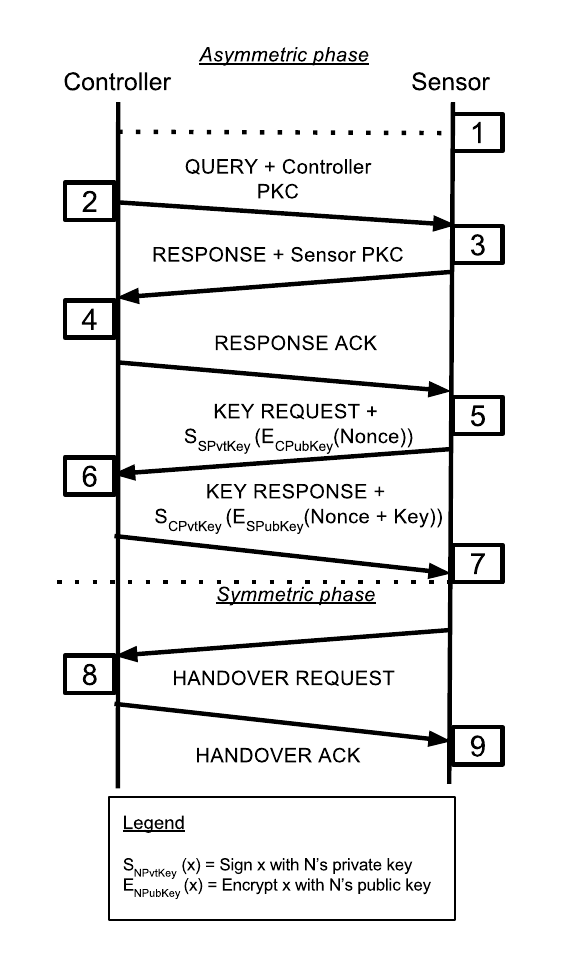
\begin{tikzpicture}[y=0.80pt, x=0.8pt,yscale=-0.7,xscale=0.7, inner sep=0pt, outer sep=0pt,
line cap=rect,miter limit=10.00]
  \path[fill=black,fill opacity=0.000,nonzero rule] (0.0000,0.0000) --
    (299.2152,0.0000) -- (299.2152,575.0892) -- (0.0000,575.0892) -- cycle;
  \path[fill=black,fill opacity=0.000,nonzero rule] (199.0892,8.0000) --
    (314.4278,8.0000) -- (314.4278,56.0000) -- (199.0892,56.0000) -- cycle;
  \path[fill=black,nonzero rule] (232.1296,28.6725) -- (233.5671,28.5475) ..
    controls (233.6296,29.1204) and (233.7859,29.5944) .. (234.0359,29.9694) ..
    controls (234.2859,30.3340) and (234.6713,30.6308) .. (235.1921,30.8600) ..
    controls (235.7130,31.0787) and (236.2963,31.1881) .. (236.9421,31.1881) ..
    controls (237.5255,31.1881) and (238.0359,31.1048) .. (238.4734,30.9381) ..
    controls (238.9213,30.7610) and (239.2494,30.5267) .. (239.4577,30.2350) ..
    controls (239.6765,29.9329) and (239.7859,29.6048) .. (239.7859,29.2506) ..
    controls (239.7859,28.8860) and (239.6817,28.5735) .. (239.4734,28.3131) ..
    controls (239.2650,28.0423) and (238.9213,27.8131) .. (238.4421,27.6256) ..
    controls (238.1400,27.5110) and (237.4630,27.3287) .. (236.4109,27.0787) ..
    controls (235.3588,26.8183) and (234.6192,26.5787) .. (234.1921,26.3600) ..
    controls (233.6505,26.0683) and (233.2442,25.7142) .. (232.9734,25.2975) ..
    controls (232.7025,24.8704) and (232.5671,24.3912) .. (232.5671,23.8600) ..
    controls (232.5671,23.2871) and (232.7286,22.7506) .. (233.0515,22.2506) ..
    controls (233.3848,21.7402) and (233.8640,21.3548) .. (234.4890,21.0944) ..
    controls (235.1244,20.8340) and (235.8275,20.7037) .. (236.5984,20.7037) ..
    controls (237.4525,20.7037) and (238.2025,20.8444) .. (238.8484,21.1256) ..
    controls (239.4942,21.3965) and (239.9890,21.7975) .. (240.3327,22.3287) ..
    controls (240.6869,22.8600) and (240.8796,23.4590) .. (240.9109,24.1256) --
    (239.4577,24.2350) .. controls (239.3744,23.5162) and (239.1088,22.9746) ..
    (238.6609,22.6100) .. controls (238.2130,22.2350) and (237.5463,22.0475) ..
    (236.6609,22.0475) .. controls (235.7442,22.0475) and (235.0775,22.2142) ..
    (234.6609,22.5475) .. controls (234.2442,22.8808) and (234.0359,23.2871) ..
    (234.0359,23.7662) .. controls (234.0359,24.1725) and (234.1817,24.5110) ..
    (234.4734,24.7819) .. controls (234.7650,25.0423) and (235.5255,25.3131) ..
    (236.7546,25.5944) .. controls (237.9942,25.8756) and (238.8432,26.1204) ..
    (239.3015,26.3287) .. controls (239.9682,26.6308) and (240.4577,27.0215) ..
    (240.7702,27.5006) .. controls (241.0932,27.9694) and (241.2546,28.5110) ..
    (241.2546,29.1256) .. controls (241.2546,29.7298) and (241.0775,30.3027) ..
    (240.7234,30.8444) .. controls (240.3796,31.3860) and (239.8796,31.8079) ..
    (239.2234,32.1100) .. controls (238.5671,32.4121) and (237.8327,32.5631) ..
    (237.0202,32.5631) .. controls (235.9786,32.5631) and (235.1088,32.4121) ..
    (234.4109,32.1100) .. controls (233.7130,31.7975) and (233.1609,31.3392) ..
    (232.7546,30.7350) .. controls (232.3588,30.1308) and (232.1505,29.4433) ..
    (232.1296,28.6725) -- cycle(248.8171,29.6881) -- (250.2702,29.8600) ..
    controls (250.0411,30.7142) and (249.6140,31.3756) .. (248.9890,31.8444) ..
    controls (248.3744,32.3131) and (247.5880,32.5475) .. (246.6296,32.5475) ..
    controls (245.4109,32.5475) and (244.4473,32.1725) .. (243.7390,31.4225) ..
    controls (243.0307,30.6725) and (242.6765,29.6256) .. (242.6765,28.2819) ..
    controls (242.6765,26.8860) and (243.0359,25.8027) .. (243.7546,25.0319) ..
    controls (244.4734,24.2610) and (245.4057,23.8756) .. (246.5515,23.8756) ..
    controls (247.6557,23.8756) and (248.5567,24.2558) .. (249.2546,25.0162) ..
    controls (249.9630,25.7662) and (250.3171,26.8235) .. (250.3171,28.1881) ..
    controls (250.3171,28.2715) and (250.3171,28.3965) .. (250.3171,28.5631) --
    (244.1296,28.5631) .. controls (244.1817,29.4798) and (244.4369,30.1829) ..
    (244.8952,30.6725) .. controls (245.3640,31.1517) and (245.9421,31.3912) ..
    (246.6296,31.3912) .. controls (247.1505,31.3912) and (247.5932,31.2558) ..
    (247.9577,30.9850) .. controls (248.3223,30.7142) and (248.6088,30.2819) ..
    (248.8171,29.6881) -- cycle(244.2077,27.4069) -- (248.8327,27.4069) ..
    controls (248.7702,26.7090) and (248.5932,26.1881) .. (248.3015,25.8444) ..
    controls (247.8536,25.3027) and (247.2755,25.0319) .. (246.5671,25.0319) ..
    controls (245.9213,25.0319) and (245.3744,25.2506) .. (244.9265,25.6881) ..
    controls (244.4890,26.1152) and (244.2494,26.6881) .. (244.2077,27.4069) --
    cycle(252.0437,32.3600) -- (252.0437,24.0631) -- (253.3093,24.0631) --
    (253.3093,25.2350) .. controls (253.9135,24.3287) and (254.7937,23.8756) ..
    (255.9499,23.8756) .. controls (256.4499,23.8756) and (256.9083,23.9642) ..
    (257.3249,24.1412) .. controls (257.7416,24.3183) and (258.0541,24.5527) ..
    (258.2624,24.8444) .. controls (258.4708,25.1360) and (258.6166,25.4850) ..
    (258.6999,25.8912) .. controls (258.7520,26.1517) and (258.7781,26.6048) ..
    (258.7781,27.2506) -- (258.7781,32.3600) -- (257.3718,32.3600) --
    (257.3718,27.3131) .. controls (257.3718,26.7402) and (257.3145,26.3131) ..
    (257.1999,26.0319) .. controls (257.0958,25.7402) and (256.9031,25.5110) ..
    (256.6218,25.3444) .. controls (256.3510,25.1777) and (256.0281,25.0944) ..
    (255.6531,25.0944) .. controls (255.0489,25.0944) and (254.5281,25.2871) ..
    (254.0906,25.6725) .. controls (253.6635,26.0475) and (253.4499,26.7662) ..
    (253.4499,27.8287) -- (253.4499,32.3600) -- (252.0437,32.3600) --
    cycle(260.3796,29.8756) -- (261.7703,29.6569) .. controls (261.8432,30.2194)
    and (262.0567,30.6517) .. (262.4109,30.9537) .. controls (262.7755,31.2454)
    and (263.2755,31.3912) .. (263.9109,31.3912) .. controls (264.5567,31.3912)
    and (265.0359,31.2610) .. (265.3484,31.0006) .. controls (265.6609,30.7298)
    and (265.8171,30.4173) .. (265.8171,30.0631) .. controls (265.8171,29.7506)
    and (265.6817,29.5006) .. (265.4109,29.3131) .. controls (265.2130,29.1881)
    and (264.7338,29.0319) .. (263.9734,28.8444) .. controls (262.9421,28.5840)
    and (262.2234,28.3600) .. (261.8171,28.1725) .. controls (261.4213,27.9746)
    and (261.1192,27.7090) .. (260.9109,27.3756) .. controls (260.7130,27.0423)
    and (260.6140,26.6725) .. (260.6140,26.2662) .. controls (260.6140,25.8912)
    and (260.6973,25.5475) .. (260.8640,25.2350) .. controls (261.0307,24.9225)
    and (261.2598,24.6621) .. (261.5515,24.4537) .. controls (261.7703,24.2871)
    and (262.0671,24.1517) .. (262.4421,24.0475) .. controls (262.8276,23.9329)
    and (263.2338,23.8756) .. (263.6609,23.8756) .. controls (264.3171,23.8756)
    and (264.8901,23.9694) .. (265.3796,24.1569) .. controls (265.8692,24.3444)
    and (266.2286,24.5996) .. (266.4578,24.9225) .. controls (266.6973,25.2350)
    and (266.8640,25.6621) .. (266.9578,26.2037) -- (265.5828,26.3912) .. controls
    (265.5203,25.9642) and (265.3380,25.6308) .. (265.0359,25.3912) .. controls
    (264.7338,25.1517) and (264.3119,25.0319) .. (263.7703,25.0319) .. controls
    (263.1244,25.0319) and (262.6609,25.1412) .. (262.3796,25.3600) .. controls
    (262.1088,25.5683) and (261.9734,25.8131) .. (261.9734,26.0944) .. controls
    (261.9734,26.2819) and (262.0307,26.4485) .. (262.1453,26.5944) .. controls
    (262.2598,26.7402) and (262.4369,26.8652) .. (262.6765,26.9694) .. controls
    (262.8223,27.0215) and (263.2390,27.1412) .. (263.9265,27.3287) .. controls
    (264.9161,27.5892) and (265.6088,27.8079) .. (266.0046,27.9850) .. controls
    (266.4005,28.1517) and (266.7078,28.3965) .. (266.9265,28.7194) .. controls
    (267.1557,29.0423) and (267.2703,29.4433) .. (267.2703,29.9225) .. controls
    (267.2703,30.3912) and (267.1296,30.8340) .. (266.8484,31.2506) .. controls
    (266.5776,31.6569) and (266.1817,31.9746) .. (265.6609,32.2037) .. controls
    (265.1505,32.4329) and (264.5723,32.5475) .. (263.9265,32.5475) .. controls
    (262.8432,32.5475) and (262.0203,32.3235) .. (261.4578,31.8756) .. controls
    (260.8953,31.4277) and (260.5359,30.7610) .. (260.3796,29.8756) --
    cycle(268.4109,28.2037) .. controls (268.4109,26.6725) and (268.8380,25.5371)
    .. (269.6921,24.7975) .. controls (270.4109,24.1829) and (271.2807,23.8756) ..
    (272.3015,23.8756) .. controls (273.4473,23.8756) and (274.3796,24.2506) ..
    (275.0984,25.0006) .. controls (275.8276,25.7402) and (276.1921,26.7715) ..
    (276.1921,28.0944) .. controls (276.1921,29.1569) and (276.0307,29.9954) ..
    (275.7078,30.6100) .. controls (275.3848,31.2246) and (274.9161,31.7037) ..
    (274.3015,32.0475) .. controls (273.6973,32.3808) and (273.0307,32.5475) ..
    (272.3015,32.5475) .. controls (271.1453,32.5475) and (270.2078,32.1777) ..
    (269.4890,31.4381) .. controls (268.7703,30.6881) and (268.4109,29.6100) ..
    (268.4109,28.2037) -- cycle(269.8640,28.2037) .. controls (269.8640,29.2662)
    and (270.0932,30.0631) .. (270.5515,30.5944) .. controls (271.0203,31.1256)
    and (271.6036,31.3912) .. (272.3015,31.3912) .. controls (272.9994,31.3912)
    and (273.5776,31.1256) .. (274.0359,30.5944) .. controls (274.5046,30.0631)
    and (274.7390,29.2506) .. (274.7390,28.1569) .. controls (274.7390,27.1360)
    and (274.5046,26.3600) .. (274.0359,25.8287) .. controls (273.5776,25.2975)
    and (272.9994,25.0319) .. (272.3015,25.0319) .. controls (271.6036,25.0319)
    and (271.0203,25.2975) .. (270.5515,25.8287) .. controls (270.0932,26.3496)
    and (269.8640,27.1412) .. (269.8640,28.2037) -- cycle(277.8249,32.3600) --
    (277.8249,24.0631) -- (279.0906,24.0631) -- (279.0906,25.3131) .. controls
    (279.4135,24.7298) and (279.7104,24.3444) .. (279.9812,24.1569) .. controls
    (280.2520,23.9694) and (280.5541,23.8756) .. (280.8874,23.8756) .. controls
    (281.3562,23.8756) and (281.8354,24.0267) .. (282.3249,24.3287) --
    (281.8406,25.6256) .. controls (281.4968,25.4277) and (281.1531,25.3287) ..
    (280.8093,25.3287) .. controls (280.5072,25.3287) and (280.2312,25.4225) ..
    (279.9812,25.6100) .. controls (279.7416,25.7871) and (279.5697,26.0423) ..
    (279.4656,26.3756) .. controls (279.3093,26.8756) and (279.2312,27.4225) ..
    (279.2312,28.0162) -- (279.2312,32.3600) -- (277.8249,32.3600) -- cycle;
  \path[fill=black,fill opacity=0.000,nonzero rule] (42.4278,59.1457) --
    (259.6562,60.0276);
  \path[draw=black,dash pattern=on 1.60pt off 4.80pt,line join=round,line
    cap=butt,nonzero rule,line width=1.600pt] (42.4278,59.1457) --
    (259.6562,60.0276);
  \path[fill=black,fill opacity=0.000,nonzero rule] (43.0420,104.7559) --
    (259.0420,119.2441);
  \path[draw=black,line join=round,line cap=butt,even odd rule,line width=1.600pt]
    (43.0420,104.7559) -- (247.0689,118.4410);
  \path[draw=black,fill=black,line cap=butt,even odd rule,line width=1.600pt]
    (246.8478,121.7371) -- (256.1248,119.0484) -- (247.2900,115.1449) -- cycle;
  \path[fill=black,fill opacity=0.000,nonzero rule] (61.5722,64.3779) --
    (229.5722,64.3779) -- (229.5722,96.3779) -- (61.5722,96.3779) -- cycle;
  \path[fill=black,nonzero rule] (93.4531,85.1780) .. controls (94.0156,85.5738)
    and (94.5416,85.8602) .. (95.0312,86.0373) -- (94.6718,86.8967) .. controls
    (93.9947,86.6571) and (93.3281,86.2769) .. (92.6718,85.7561) .. controls
    (91.9739,86.1415) and (91.2083,86.3342) .. (90.3749,86.3342) .. controls
    (89.5312,86.3342) and (88.7656,86.1311) .. (88.0781,85.7248) .. controls
    (87.4010,85.3186) and (86.8749,84.7509) .. (86.4999,84.0217) .. controls
    (86.1354,83.2821) and (85.9531,82.4488) .. (85.9531,81.5217) .. controls
    (85.9531,80.6050) and (86.1354,79.7717) .. (86.4999,79.0217) .. controls
    (86.8749,78.2613) and (87.4062,77.6884) .. (88.0937,77.3030) .. controls
    (88.7812,76.9071) and (89.5520,76.7092) .. (90.4062,76.7092) .. controls
    (91.2604,76.7092) and (92.0312,76.9123) .. (92.7187,77.3186) .. controls
    (93.4166,77.7248) and (93.9427,78.2977) .. (94.2968,79.0373) .. controls
    (94.6614,79.7665) and (94.8437,80.5946) .. (94.8437,81.5217) .. controls
    (94.8437,82.2821) and (94.7291,82.9696) .. (94.4999,83.5842) .. controls
    (94.2708,84.1988) and (93.9218,84.7300) .. (93.4531,85.1780) --
    cycle(90.7343,83.5998) .. controls (91.4427,83.8082) and (92.0312,84.1050) ..
    (92.4999,84.4905) .. controls (93.2187,83.8342) and (93.5781,82.8446) ..
    (93.5781,81.5217) .. controls (93.5781,80.7613) and (93.4479,80.0998) ..
    (93.1874,79.5373) .. controls (92.9374,78.9748) and (92.5624,78.5425) ..
    (92.0624,78.2405) .. controls (91.5729,77.9280) and (91.0208,77.7717) ..
    (90.4062,77.7717) .. controls (89.4895,77.7717) and (88.7291,78.0842) ..
    (88.1249,78.7092) .. controls (87.5208,79.3342) and (87.2187,80.2717) ..
    (87.2187,81.5217) .. controls (87.2187,82.7300) and (87.5156,83.6623) ..
    (88.1093,84.3186) .. controls (88.7135,84.9644) and (89.4791,85.2873) ..
    (90.4062,85.2873) .. controls (90.8541,85.2873) and (91.2708,85.2040) ..
    (91.6562,85.0373) .. controls (91.2708,84.7873) and (90.8645,84.6102) ..
    (90.4374,84.5061) -- (90.7343,83.5998) -- cycle(102.8670,76.8655) --
    (104.1014,76.8655) -- (104.1014,82.2561) .. controls (104.1014,83.1832) and
    (103.9920,83.9227) .. (103.7732,84.4748) .. controls (103.5649,85.0269) and
    (103.1847,85.4748) .. (102.6326,85.8186) .. controls (102.0805,86.1623) and
    (101.3566,86.3342) .. (100.4607,86.3342) .. controls (99.5857,86.3342) and
    (98.8722,86.1832) .. (98.3201,85.8811) .. controls (97.7680,85.5790) and
    (97.3722,85.1467) .. (97.1326,84.5842) .. controls (96.8930,84.0113) and
    (96.7732,83.2352) .. (96.7732,82.2561) -- (96.7732,76.8655) --
    (98.0076,76.8655) -- (98.0076,82.2405) .. controls (98.0076,83.0530) and
    (98.0805,83.6519) .. (98.2264,84.0373) .. controls (98.3826,84.4123) and
    (98.6430,84.7040) .. (99.0076,84.9123) .. controls (99.3722,85.1207) and
    (99.8201,85.2248) .. (100.3514,85.2248) .. controls (101.2576,85.2248) and
    (101.9035,85.0217) .. (102.2889,84.6155) .. controls (102.6743,84.1988) and
    (102.8670,83.4071) .. (102.8670,82.2405) -- (102.8670,76.8655) --
    cycle(106.4140,86.1780) -- (106.4140,76.8655) -- (113.1328,76.8655) --
    (113.1328,77.9748) -- (107.6484,77.9748) -- (107.6484,80.8186) --
    (112.7890,80.8186) -- (112.7890,81.9123) -- (107.6484,81.9123) --
    (107.6484,85.0842) -- (113.3515,85.0842) -- (113.3515,86.1780) --
    (106.4140,86.1780) -- cycle(115.2882,86.1780) -- (115.2882,76.8655) --
    (119.4132,76.8655) .. controls (120.2465,76.8655) and (120.8767,76.9540) ..
    (121.3038,77.1311) .. controls (121.7413,77.2977) and (122.0902,77.5946) ..
    (122.3507,78.0217) .. controls (122.6111,78.4384) and (122.7413,78.9019) ..
    (122.7413,79.4123) .. controls (122.7413,80.0686) and (122.5225,80.6259) ..
    (122.0850,81.0842) .. controls (121.6579,81.5321) and (121.0017,81.8186) ..
    (120.1163,81.9436) .. controls (120.4392,82.0998) and (120.6840,82.2561) ..
    (120.8507,82.4123) .. controls (121.2152,82.7352) and (121.5590,83.1467) ..
    (121.8819,83.6467) -- (123.4913,86.1780) -- (121.9444,86.1780) --
    (120.7100,84.2405) .. controls (120.3559,83.6780) and (120.0590,83.2509) ..
    (119.8194,82.9592) .. controls (119.5902,82.6675) and (119.3819,82.4644) ..
    (119.1944,82.3498) .. controls (119.0173,82.2248) and (118.8350,82.1363) ..
    (118.6475,82.0842) .. controls (118.5017,82.0634) and (118.2725,82.0530) ..
    (117.9600,82.0530) -- (116.5225,82.0530) -- (116.5225,86.1780) --
    (115.2882,86.1780) -- cycle(116.5225,80.9748) -- (119.1788,80.9748) ..
    controls (119.7413,80.9748) and (120.1788,80.9175) .. (120.4913,80.8030) ..
    controls (120.8142,80.6884) and (121.0538,80.5061) .. (121.2100,80.2561) ..
    controls (121.3767,79.9957) and (121.4600,79.7144) .. (121.4600,79.4123) ..
    controls (121.4600,78.9748) and (121.2986,78.6155) .. (120.9757,78.3342) ..
    controls (120.6632,78.0425) and (120.1632,77.8967) .. (119.4757,77.8967) --
    (116.5225,77.8967) -- (116.5225,80.9748) -- cycle(127.5227,86.1780) --
    (127.5227,82.2405) -- (123.9289,76.8655) -- (125.4289,76.8655) --
    (127.2727,79.6780) .. controls (127.6060,80.1988) and (127.9185,80.7248) ..
    (128.2102,81.2561) .. controls (128.4914,80.7665) and (128.8300,80.2196) ..
    (129.2258,79.6155) -- (131.0383,76.8655) -- (132.4602,76.8655) --
    (128.7570,82.2405) -- (128.7570,86.1780) -- (127.5227,86.1780) --
    cycle(139.7404,84.6780) -- (139.7404,82.1155) -- (137.2092,82.1155) --
    (137.2092,81.0530) -- (139.7404,81.0530) -- (139.7404,78.5217) --
    (140.8185,78.5217) -- (140.8185,81.0530) -- (143.3654,81.0530) --
    (143.3654,82.1155) -- (140.8185,82.1155) -- (140.8185,84.6780) --
    (139.7404,84.6780) -- cycle(155.6174,82.9123) -- (156.8518,83.2248) ..
    controls (156.5914,84.2352) and (156.1227,85.0061) .. (155.4456,85.5373) ..
    controls (154.7789,86.0686) and (153.9612,86.3342) .. (152.9924,86.3342) ..
    controls (151.9924,86.3342) and (151.1747,86.1311) .. (150.5393,85.7248) ..
    controls (149.9143,85.3186) and (149.4352,84.7300) .. (149.1018,83.9592) ..
    controls (148.7789,83.1780) and (148.6174,82.3446) .. (148.6174,81.4592) ..
    controls (148.6174,80.4905) and (148.8049,79.6467) .. (149.1799,78.9280) ..
    controls (149.5549,78.1988) and (150.0810,77.6467) .. (150.7581,77.2717) ..
    controls (151.4456,76.8967) and (152.2008,76.7092) .. (153.0237,76.7092) ..
    controls (153.9508,76.7092) and (154.7320,76.9488) .. (155.3674,77.4280) ..
    controls (156.0029,77.8967) and (156.4456,78.5634) .. (156.6956,79.4280) --
    (155.4768,79.7092) .. controls (155.2581,79.0321) and (154.9456,78.5425) ..
    (154.5393,78.2405) .. controls (154.1331,77.9280) and (153.6174,77.7717) ..
    (152.9924,77.7717) .. controls (152.2737,77.7717) and (151.6747,77.9436) ..
    (151.1956,78.2873) .. controls (150.7164,78.6311) and (150.3779,79.0894) ..
    (150.1799,79.6623) .. controls (149.9924,80.2352) and (149.8987,80.8290) ..
    (149.8987,81.4436) .. controls (149.8987,82.2352) and (150.0133,82.9280) ..
    (150.2424,83.5217) .. controls (150.4716,84.1155) and (150.8258,84.5582) ..
    (151.3049,84.8498) .. controls (151.7945,85.1415) and (152.3258,85.2873) ..
    (152.8987,85.2873) .. controls (153.5862,85.2873) and (154.1695,85.0894) ..
    (154.6487,84.6936) .. controls (155.1279,84.2873) and (155.4508,83.6936) ..
    (155.6174,82.9123) -- cycle(158.0395,82.8030) .. controls (158.0395,81.5530)
    and (158.3832,80.6311) .. (159.0707,80.0373) .. controls (159.6541,79.5373)
    and (160.3624,79.2873) .. (161.1957,79.2873) .. controls (162.1228,79.2873)
    and (162.8780,79.5894) .. (163.4613,80.1936) .. controls (164.0551,80.7977)
    and (164.3520,81.6363) .. (164.3520,82.7092) .. controls (164.3520,83.5738)
    and (164.2218,84.2561) .. (163.9613,84.7561) .. controls (163.7009,85.2561)
    and (163.3207,85.6467) .. (162.8207,85.9280) .. controls (162.3207,86.1988)
    and (161.7791,86.3342) .. (161.1957,86.3342) .. controls (160.2478,86.3342)
    and (159.4822,86.0321) .. (158.8988,85.4280) .. controls (158.3259,84.8238)
    and (158.0395,83.9488) .. (158.0395,82.8030) -- cycle(159.2113,82.8030) ..
    controls (159.2113,83.6675) and (159.3988,84.3186) .. (159.7738,84.7561) ..
    controls (160.1488,85.1832) and (160.6228,85.3967) .. (161.1957,85.3967) ..
    controls (161.7582,85.3967) and (162.2270,85.1832) .. (162.6020,84.7561) ..
    controls (162.9874,84.3186) and (163.1801,83.6571) .. (163.1801,82.7717) ..
    controls (163.1801,81.9384) and (162.9874,81.3082) .. (162.6020,80.8811) ..
    controls (162.2270,80.4436) and (161.7582,80.2248) .. (161.1957,80.2248) ..
    controls (160.6228,80.2248) and (160.1488,80.4384) .. (159.7738,80.8655) ..
    controls (159.3988,81.2925) and (159.2113,81.9384) .. (159.2113,82.8030) --
    cycle(165.8738,86.1780) -- (165.8738,79.4436) -- (166.9051,79.4436) --
    (166.9051,80.3967) .. controls (167.3947,79.6571) and (168.1082,79.2873) ..
    (169.0457,79.2873) .. controls (169.4519,79.2873) and (169.8217,79.3602) ..
    (170.1551,79.5061) .. controls (170.4988,79.6519) and (170.7540,79.8446) ..
    (170.9207,80.0842) .. controls (171.0978,80.3134) and (171.2176,80.5946) ..
    (171.2801,80.9280) .. controls (171.3217,81.1363) and (171.3426,81.5061) ..
    (171.3426,82.0373) -- (171.3426,86.1780) -- (170.2019,86.1780) --
    (170.2019,82.0842) .. controls (170.2019,81.6155) and (170.1551,81.2665) ..
    (170.0613,81.0373) .. controls (169.9780,80.8082) and (169.8217,80.6259) ..
    (169.5926,80.4905) .. controls (169.3738,80.3446) and (169.1134,80.2717) ..
    (168.8113,80.2717) .. controls (168.3217,80.2717) and (167.8999,80.4280) ..
    (167.5457,80.7405) .. controls (167.1915,81.0425) and (167.0144,81.6259) ..
    (167.0144,82.4905) -- (167.0144,86.1780) -- (165.8738,86.1780) --
    cycle(175.7863,85.1623) -- (175.9425,86.1623) .. controls (175.6196,86.2352)
    and (175.3332,86.2717) .. (175.0832,86.2717) .. controls (174.6665,86.2717)
    and (174.3436,86.2040) .. (174.1144,86.0686) .. controls (173.8853,85.9332)
    and (173.7238,85.7613) .. (173.6300,85.5530) .. controls (173.5363,85.3342)
    and (173.4894,84.8863) .. (173.4894,84.2092) -- (173.4894,80.3186) --
    (172.6613,80.3186) -- (172.6613,79.4436) -- (173.4894,79.4436) --
    (173.4894,77.7717) -- (174.6300,77.0842) -- (174.6300,79.4436) --
    (175.7863,79.4436) -- (175.7863,80.3186) -- (174.6300,80.3186) --
    (174.6300,84.2717) .. controls (174.6300,84.5946) and (174.6509,84.8030) ..
    (174.6925,84.8967) .. controls (174.7342,84.9905) and (174.7967,85.0634) ..
    (174.8800,85.1155) .. controls (174.9738,85.1675) and (175.1040,85.1936) ..
    (175.2707,85.1936) .. controls (175.4061,85.1936) and (175.5780,85.1832) ..
    (175.7863,85.1623) -- cycle(176.9737,86.1780) -- (176.9737,79.4436) --
    (178.0049,79.4436) -- (178.0049,80.4592) .. controls (178.2653,79.9800) and
    (178.5049,79.6675) .. (178.7237,79.5217) .. controls (178.9528,79.3655) and
    (179.1976,79.2873) .. (179.4580,79.2873) .. controls (179.8435,79.2873) and
    (180.2341,79.4071) .. (180.6299,79.6467) -- (180.2393,80.7092) .. controls
    (179.9580,80.5425) and (179.6820,80.4592) .. (179.4112,80.4592) .. controls
    (179.1612,80.4592) and (178.9320,80.5373) .. (178.7237,80.6936) .. controls
    (178.5257,80.8394) and (178.3851,81.0477) .. (178.3018,81.3186) .. controls
    (178.1768,81.7248) and (178.1143,82.1675) .. (178.1143,82.6467) --
    (178.1143,86.1780) -- (176.9737,86.1780) -- cycle(181.0058,82.8030) ..
    controls (181.0058,81.5530) and (181.3495,80.6311) .. (182.0370,80.0373) ..
    controls (182.6204,79.5373) and (183.3287,79.2873) .. (184.1620,79.2873) ..
    controls (185.0891,79.2873) and (185.8443,79.5894) .. (186.4277,80.1936) ..
    controls (187.0214,80.7977) and (187.3183,81.6363) .. (187.3183,82.7092) ..
    controls (187.3183,83.5738) and (187.1881,84.2561) .. (186.9277,84.7561) ..
    controls (186.6672,85.2561) and (186.2870,85.6467) .. (185.7870,85.9280) ..
    controls (185.2870,86.1988) and (184.7454,86.3342) .. (184.1620,86.3342) ..
    controls (183.2141,86.3342) and (182.4485,86.0321) .. (181.8652,85.4280) ..
    controls (181.2922,84.8238) and (181.0058,83.9488) .. (181.0058,82.8030) --
    cycle(182.1777,82.8030) .. controls (182.1777,83.6675) and (182.3652,84.3186)
    .. (182.7402,84.7561) .. controls (183.1152,85.1832) and (183.5891,85.3967) ..
    (184.1620,85.3967) .. controls (184.7245,85.3967) and (185.1933,85.1832) ..
    (185.5683,84.7561) .. controls (185.9537,84.3186) and (186.1464,83.6571) ..
    (186.1464,82.7717) .. controls (186.1464,81.9384) and (185.9537,81.3082) ..
    (185.5683,80.8811) .. controls (185.1933,80.4436) and (184.7245,80.2248) ..
    (184.1620,80.2248) .. controls (183.5891,80.2248) and (183.1152,80.4384) ..
    (182.7402,80.8655) .. controls (182.3652,81.2925) and (182.1777,81.9384) ..
    (182.1777,82.8030) -- cycle(188.8089,86.1780) -- (188.8089,76.8655) --
    (189.9495,76.8655) -- (189.9495,86.1780) -- (188.8089,86.1780) --
    cycle(191.7700,86.1780) -- (191.7700,76.8655) -- (192.9106,76.8655) --
    (192.9106,86.1780) -- (191.7700,86.1780) -- cycle(199.3717,84.0061) --
    (200.5592,84.1467) .. controls (200.3717,84.8446) and (200.0227,85.3863) ..
    (199.5123,85.7717) .. controls (199.0123,86.1467) and (198.3717,86.3342) ..
    (197.5904,86.3342) .. controls (196.6009,86.3342) and (195.8144,86.0321) ..
    (195.2311,85.4280) .. controls (194.6581,84.8134) and (194.3717,83.9592) ..
    (194.3717,82.8655) .. controls (194.3717,81.7300) and (194.6634,80.8498) ..
    (195.2467,80.2248) .. controls (195.8404,79.5998) and (196.6009,79.2873) ..
    (197.5279,79.2873) .. controls (198.4342,79.2873) and (199.1686,79.5946) ..
    (199.7311,80.2092) .. controls (200.3040,80.8238) and (200.5904,81.6832) ..
    (200.5904,82.7873) .. controls (200.5904,82.8602) and (200.5904,82.9644) ..
    (200.5904,83.0998) -- (195.5592,83.0998) .. controls (195.6009,83.8394) and
    (195.8092,84.4071) .. (196.1842,84.8030) .. controls (196.5592,85.1988) and
    (197.0279,85.3967) .. (197.5904,85.3967) .. controls (198.0175,85.3967) and
    (198.3769,85.2873) .. (198.6686,85.0686) .. controls (198.9706,84.8394) and
    (199.2050,84.4852) .. (199.3717,84.0061) -- cycle(195.6217,82.1623) --
    (199.3873,82.1623) .. controls (199.3352,81.5894) and (199.1894,81.1623) ..
    (198.9498,80.8811) .. controls (198.5852,80.4436) and (198.1165,80.2248) ..
    (197.5436,80.2248) .. controls (197.0123,80.2248) and (196.5696,80.4019) ..
    (196.2154,80.7561) .. controls (195.8613,81.0998) and (195.6634,81.5686) ..
    (195.6217,82.1623) -- cycle(202.1592,86.1780) -- (202.1592,79.4436) --
    (203.1904,79.4436) -- (203.1904,80.4592) .. controls (203.4508,79.9800) and
    (203.6904,79.6675) .. (203.9092,79.5217) .. controls (204.1383,79.3655) and
    (204.3831,79.2873) .. (204.6435,79.2873) .. controls (205.0290,79.2873) and
    (205.4196,79.4071) .. (205.8154,79.6467) -- (205.4248,80.7092) .. controls
    (205.1435,80.5425) and (204.8675,80.4592) .. (204.5967,80.4592) .. controls
    (204.3467,80.4592) and (204.1175,80.5373) .. (203.9092,80.6936) .. controls
    (203.7112,80.8394) and (203.5706,81.0477) .. (203.4873,81.3186) .. controls
    (203.3623,81.7248) and (203.2998,82.1675) .. (203.2998,82.6467) --
    (203.2998,86.1780) -- (202.1592,86.1780) -- cycle;
  \path[fill=black,nonzero rule] (132.8698,102.1780) -- (132.8698,92.8655) --
    (136.3855,92.8655) .. controls (137.0000,92.8655) and (137.4688,92.8967) ..
    (137.7917,92.9592) .. controls (138.2500,93.0321) and (138.6355,93.1780) ..
    (138.9480,93.3967) .. controls (139.2605,93.6050) and (139.5105,93.9019) ..
    (139.6980,94.2873) .. controls (139.8855,94.6727) and (139.9792,95.0998) ..
    (139.9792,95.5686) .. controls (139.9792,96.3602) and (139.7240,97.0321) ..
    (139.2136,97.5842) .. controls (138.7136,98.1259) and (137.8073,98.3967) ..
    (136.4948,98.3967) -- (134.1042,98.3967) -- (134.1042,102.1780) --
    (132.8698,102.1780) -- cycle(134.1042,97.3030) -- (136.5105,97.3030) ..
    controls (137.3021,97.3030) and (137.8646,97.1571) .. (138.1980,96.8655) ..
    controls (138.5417,96.5634) and (138.7136,96.1415) .. (138.7136,95.5998) ..
    controls (138.7136,95.2144) and (138.6146,94.8863) .. (138.4167,94.6155) ..
    controls (138.2188,94.3342) and (137.9584,94.1467) .. (137.6355,94.0530) ..
    controls (137.4271,94.0009) and (137.0417,93.9748) .. (136.4792,93.9748) --
    (134.1042,93.9748) -- (134.1042,97.3030) -- cycle(141.7127,102.1780) --
    (141.7127,92.8655) -- (142.9471,92.8655) -- (142.9471,97.4905) --
    (147.5721,92.8655) -- (149.2283,92.8655) -- (145.3377,96.6467) --
    (149.4002,102.1780) -- (147.7752,102.1780) -- (144.4627,97.4748) --
    (142.9471,98.9592) -- (142.9471,102.1780) -- (141.7127,102.1780) --
    cycle(157.2900,98.9123) -- (158.5244,99.2248) .. controls (158.2639,100.2352)
    and (157.7952,101.0061) .. (157.1181,101.5373) .. controls (156.4514,102.0686)
    and (155.6337,102.3342) .. (154.6650,102.3342) .. controls (153.6650,102.3342)
    and (152.8473,102.1311) .. (152.2119,101.7248) .. controls (151.5869,101.3186)
    and (151.1077,100.7300) .. (150.7744,99.9592) .. controls (150.4514,99.1780)
    and (150.2900,98.3446) .. (150.2900,97.4592) .. controls (150.2900,96.4905)
    and (150.4775,95.6467) .. (150.8525,94.9280) .. controls (151.2275,94.1988)
    and (151.7535,93.6467) .. (152.4306,93.2717) .. controls (153.1181,92.8967)
    and (153.8733,92.7092) .. (154.6962,92.7092) .. controls (155.6233,92.7092)
    and (156.4046,92.9488) .. (157.0400,93.4280) .. controls (157.6754,93.8967)
    and (158.1181,94.5634) .. (158.3681,95.4280) -- (157.1494,95.7092) .. controls
    (156.9306,95.0321) and (156.6181,94.5425) .. (156.2119,94.2405) .. controls
    (155.8056,93.9280) and (155.2900,93.7717) .. (154.6650,93.7717) .. controls
    (153.9462,93.7717) and (153.3473,93.9436) .. (152.8681,94.2873) .. controls
    (152.3889,94.6311) and (152.0504,95.0894) .. (151.8525,95.6623) .. controls
    (151.6650,96.2352) and (151.5712,96.8290) .. (151.5712,97.4436) .. controls
    (151.5712,98.2352) and (151.6858,98.9280) .. (151.9150,99.5217) .. controls
    (152.1441,100.1155) and (152.4983,100.5582) .. (152.9775,100.8498) .. controls
    (153.4671,101.1415) and (153.9983,101.2873) .. (154.5712,101.2873) .. controls
    (155.2587,101.2873) and (155.8421,101.0894) .. (156.3212,100.6936) .. controls
    (156.8004,100.2873) and (157.1233,99.6936) .. (157.2900,98.9123) -- cycle;
  \path[fill=black,fill opacity=0.000,nonzero rule] (256.9160,149.6404) --
    (42.4278,166.1444);
  \path[draw=black,line join=round,line cap=butt,even odd rule,line width=1.600pt]
    (256.9160,149.6404) -- (54.3925,165.2237);
  \path[draw=black,fill=black,line cap=butt,even odd rule,line width=1.600pt]
    (54.1390,161.9300) -- (45.3430,165.9200) -- (54.6459,168.5175) -- cycle;
  \path[fill=black,fill opacity=0.000,nonzero rule] (53.5722,121.1076) --
    (237.5722,121.1076) -- (237.5722,153.1076) -- (53.5722,153.1076) -- cycle;
  \path[fill=black,nonzero rule] (65.2914,142.9076) -- (65.2914,133.5951) --
    (69.4164,133.5951) .. controls (70.2497,133.5951) and (70.8800,133.6837) ..
    (71.3070,133.8607) .. controls (71.7445,134.0274) and (72.0935,134.3243) ..
    (72.3539,134.7514) .. controls (72.6143,135.1680) and (72.7445,135.6316) ..
    (72.7445,136.1420) .. controls (72.7445,136.7982) and (72.5258,137.3555) ..
    (72.0883,137.8139) .. controls (71.6612,138.2618) and (71.0050,138.5482) ..
    (70.1195,138.6732) .. controls (70.4425,138.8295) and (70.6872,138.9857) ..
    (70.8539,139.1420) .. controls (71.2185,139.4649) and (71.5622,139.8764) ..
    (71.8852,140.3764) -- (73.4945,142.9076) -- (71.9477,142.9076) --
    (70.7133,140.9701) .. controls (70.3591,140.4076) and (70.0622,139.9805) ..
    (69.8227,139.6889) .. controls (69.5935,139.3972) and (69.3852,139.1941) ..
    (69.1977,139.0795) .. controls (69.0206,138.9545) and (68.8383,138.8659) ..
    (68.6508,138.8139) .. controls (68.5050,138.7930) and (68.2758,138.7826) ..
    (67.9633,138.7826) -- (66.5258,138.7826) -- (66.5258,142.9076) --
    (65.2914,142.9076) -- cycle(66.5258,137.7045) -- (69.1820,137.7045) ..
    controls (69.7445,137.7045) and (70.1820,137.6472) .. (70.4945,137.5326) ..
    controls (70.8175,137.4180) and (71.0570,137.2357) .. (71.2133,136.9857) ..
    controls (71.3800,136.7253) and (71.4633,136.4441) .. (71.4633,136.1420) ..
    controls (71.4633,135.7045) and (71.3018,135.3451) .. (70.9789,135.0639) ..
    controls (70.6664,134.7722) and (70.1664,134.6264) .. (69.4789,134.6264) --
    (66.5258,134.6264) -- (66.5258,137.7045) -- cycle(74.9322,142.9076) --
    (74.9322,133.5951) -- (81.6509,133.5951) -- (81.6509,134.7045) --
    (76.1666,134.7045) -- (76.1666,137.5482) -- (81.3072,137.5482) --
    (81.3072,138.6420) -- (76.1666,138.6420) -- (76.1666,141.8139) --
    (81.8697,141.8139) -- (81.8697,142.9076) -- (74.9322,142.9076) --
    cycle(83.3688,139.9232) -- (84.5407,139.8139) .. controls (84.5928,140.2826)
    and (84.7178,140.6680) .. (84.9157,140.9701) .. controls (85.1240,141.2618)
    and (85.4365,141.5014) .. (85.8532,141.6889) .. controls (86.2803,141.8659)
    and (86.7594,141.9545) .. (87.2907,141.9545) .. controls (87.7594,141.9545)
    and (88.1709,141.8868) .. (88.5251,141.7514) .. controls (88.8897,141.6159)
    and (89.1605,141.4284) .. (89.3376,141.1889) .. controls (89.5147,140.9389)
    and (89.6032,140.6680) .. (89.6032,140.3764) .. controls (89.6032,140.0847)
    and (89.5147,139.8295) .. (89.3376,139.6107) .. controls (89.1709,139.3920)
    and (88.8949,139.2097) .. (88.5094,139.0639) .. controls (88.2594,138.9701)
    and (87.7074,138.8191) .. (86.8532,138.6107) .. controls (85.9990,138.4024)
    and (85.4001,138.2097) .. (85.0563,138.0326) .. controls (84.6084,137.8034)
    and (84.2751,137.5170) .. (84.0563,137.1732) .. controls (83.8376,136.8191)
    and (83.7282,136.4284) .. (83.7282,136.0014) .. controls (83.7282,135.5326)
    and (83.8584,135.0951) .. (84.1188,134.6889) .. controls (84.3897,134.2826)
    and (84.7803,133.9753) .. (85.2907,133.7670) .. controls (85.8115,133.5482)
    and (86.3844,133.4389) .. (87.0094,133.4389) .. controls (87.6969,133.4389)
    and (88.3011,133.5534) .. (88.8219,133.7826) .. controls (89.3532,134.0014)
    and (89.7594,134.3295) .. (90.0407,134.7670) .. controls (90.3324,135.1941)
    and (90.4886,135.6784) .. (90.5094,136.2201) -- (89.3219,136.3139) .. controls
    (89.2594,135.7201) and (89.0459,135.2774) .. (88.6813,134.9857) .. controls
    (88.3167,134.6837) and (87.7751,134.5326) .. (87.0563,134.5326) .. controls
    (86.3167,134.5326) and (85.7751,134.6680) .. (85.4313,134.9389) .. controls
    (85.0876,135.2097) and (84.9157,135.5378) .. (84.9157,135.9232) .. controls
    (84.9157,136.2566) and (85.0355,136.5326) .. (85.2751,136.7514) .. controls
    (85.5147,136.9701) and (86.1344,137.1941) .. (87.1344,137.4232) .. controls
    (88.1344,137.6420) and (88.8219,137.8347) .. (89.1969,138.0014) .. controls
    (89.7386,138.2514) and (90.1344,138.5691) .. (90.3844,138.9545) .. controls
    (90.6449,139.3399) and (90.7751,139.7826) .. (90.7751,140.2826) .. controls
    (90.7751,140.7722) and (90.6344,141.2357) .. (90.3532,141.6732) .. controls
    (90.0719,142.1107) and (89.6657,142.4545) .. (89.1344,142.7045) .. controls
    (88.6032,142.9441) and (88.0042,143.0639) .. (87.3376,143.0639) .. controls
    (86.4938,143.0639) and (85.7855,142.9441) .. (85.2126,142.7045) .. controls
    (84.6501,142.4545) and (84.2074,142.0847) .. (83.8844,141.5951) .. controls
    (83.5615,141.0951) and (83.3897,140.5378) .. (83.3688,139.9232) --
    cycle(92.6804,142.9076) -- (92.6804,133.5951) -- (96.1961,133.5951) ..
    controls (96.8107,133.5951) and (97.2794,133.6264) .. (97.6023,133.6889) ..
    controls (98.0607,133.7618) and (98.4461,133.9076) .. (98.7586,134.1264) ..
    controls (99.0711,134.3347) and (99.3211,134.6316) .. (99.5086,135.0170) ..
    controls (99.6961,135.4024) and (99.7898,135.8295) .. (99.7898,136.2982) ..
    controls (99.7898,137.0899) and (99.5346,137.7618) .. (99.0242,138.3139) ..
    controls (98.5242,138.8555) and (97.6179,139.1264) .. (96.3054,139.1264) --
    (93.9148,139.1264) -- (93.9148,142.9076) -- (92.6804,142.9076) --
    cycle(93.9148,138.0326) -- (96.3211,138.0326) .. controls (97.1127,138.0326)
    and (97.6752,137.8868) .. (98.0086,137.5951) .. controls (98.3523,137.2930)
    and (98.5242,136.8712) .. (98.5242,136.3295) .. controls (98.5242,135.9441)
    and (98.4252,135.6159) .. (98.2273,135.3451) .. controls (98.0294,135.0639)
    and (97.7690,134.8764) .. (97.4461,134.7826) .. controls (97.2377,134.7305)
    and (96.8523,134.7045) .. (96.2898,134.7045) -- (93.9148,134.7045) --
    (93.9148,138.0326) -- cycle(101.1952,138.3764) .. controls (101.1952,136.8347)
    and (101.6067,135.6264) .. (102.4296,134.7514) .. controls (103.2629,133.8764)
    and (104.3358,133.4389) .. (105.6483,133.4389) .. controls (106.5129,133.4389)
    and (107.2890,133.6472) .. (107.9765,134.0639) .. controls (108.6640,134.4701)
    and (109.1900,135.0430) .. (109.5546,135.7826) .. controls (109.9192,136.5118)
    and (110.1015,137.3399) .. (110.1015,138.2670) .. controls (110.1015,139.2149)
    and (109.9087,140.0639) .. (109.5233,140.8139) .. controls (109.1483,141.5534)
    and (108.6119,142.1159) .. (107.9140,142.5014) .. controls (107.2160,142.8764)
    and (106.4608,143.0639) .. (105.6483,143.0639) .. controls (104.7733,143.0639)
    and (103.9869,142.8555) .. (103.2890,142.4389) .. controls (102.6015,142.0118)
    and (102.0806,141.4337) .. (101.7265,140.7045) .. controls (101.3723,139.9649)
    and (101.1952,139.1889) .. (101.1952,138.3764) -- cycle(102.4608,138.3920) ..
    controls (102.4608,139.5170) and (102.7629,140.4024) .. (103.3671,141.0482) ..
    controls (103.9712,141.6941) and (104.7317,142.0170) .. (105.6483,142.0170) ..
    controls (106.5754,142.0170) and (107.3358,141.6941) .. (107.9296,141.0482) ..
    controls (108.5337,140.3920) and (108.8358,139.4649) .. (108.8358,138.2670) ..
    controls (108.8358,137.5066) and (108.7056,136.8451) .. (108.4452,136.2826) ..
    controls (108.1848,135.7097) and (107.8098,135.2722) .. (107.3202,134.9701) ..
    controls (106.8306,134.6576) and (106.2785,134.5014) .. (105.6640,134.5014) ..
    controls (104.7890,134.5014) and (104.0337,134.8034) .. (103.3983,135.4076) ..
    controls (102.7733,136.0014) and (102.4608,136.9962) .. (102.4608,138.3920) --
    cycle(111.9216,142.9076) -- (111.9216,133.5951) -- (113.1873,133.5951) --
    (118.0779,140.9076) -- (118.0779,133.5951) -- (119.2654,133.5951) --
    (119.2654,142.9076) -- (117.9998,142.9076) -- (113.1091,135.5951) --
    (113.1091,142.9076) -- (111.9216,142.9076) -- cycle(121.1405,139.9232) --
    (122.3124,139.8139) .. controls (122.3645,140.2826) and (122.4895,140.6680) ..
    (122.6874,140.9701) .. controls (122.8957,141.2618) and (123.2082,141.5014) ..
    (123.6249,141.6889) .. controls (124.0520,141.8659) and (124.5312,141.9545) ..
    (125.0624,141.9545) .. controls (125.5312,141.9545) and (125.9426,141.8868) ..
    (126.2968,141.7514) .. controls (126.6614,141.6159) and (126.9322,141.4284) ..
    (127.1093,141.1889) .. controls (127.2864,140.9389) and (127.3749,140.6680) ..
    (127.3749,140.3764) .. controls (127.3749,140.0847) and (127.2864,139.8295) ..
    (127.1093,139.6107) .. controls (126.9426,139.3920) and (126.6666,139.2097) ..
    (126.2812,139.0639) .. controls (126.0312,138.9701) and (125.4791,138.8191) ..
    (124.6249,138.6107) .. controls (123.7707,138.4024) and (123.1718,138.2097) ..
    (122.8280,138.0326) .. controls (122.3801,137.8034) and (122.0468,137.5170) ..
    (121.8280,137.1732) .. controls (121.6093,136.8191) and (121.4999,136.4284) ..
    (121.4999,136.0014) .. controls (121.4999,135.5326) and (121.6301,135.0951) ..
    (121.8905,134.6889) .. controls (122.1614,134.2826) and (122.5520,133.9753) ..
    (123.0624,133.7670) .. controls (123.5832,133.5482) and (124.1562,133.4389) ..
    (124.7812,133.4389) .. controls (125.4687,133.4389) and (126.0728,133.5534) ..
    (126.5937,133.7826) .. controls (127.1249,134.0014) and (127.5312,134.3295) ..
    (127.8124,134.7670) .. controls (128.1041,135.1941) and (128.2603,135.6784) ..
    (128.2812,136.2201) -- (127.0937,136.3139) .. controls (127.0312,135.7201) and
    (126.8176,135.2774) .. (126.4530,134.9857) .. controls (126.0884,134.6837) and
    (125.5468,134.5326) .. (124.8280,134.5326) .. controls (124.0884,134.5326) and
    (123.5468,134.6680) .. (123.2030,134.9389) .. controls (122.8593,135.2097) and
    (122.6874,135.5378) .. (122.6874,135.9232) .. controls (122.6874,136.2566) and
    (122.8072,136.5326) .. (123.0468,136.7514) .. controls (123.2864,136.9701) and
    (123.9062,137.1941) .. (124.9062,137.4232) .. controls (125.9062,137.6420) and
    (126.5937,137.8347) .. (126.9687,138.0014) .. controls (127.5103,138.2514) and
    (127.9062,138.5691) .. (128.1562,138.9545) .. controls (128.4166,139.3399) and
    (128.5468,139.7826) .. (128.5468,140.2826) .. controls (128.5468,140.7722) and
    (128.4062,141.2357) .. (128.1249,141.6732) .. controls (127.8437,142.1107) and
    (127.4374,142.4545) .. (126.9062,142.7045) .. controls (126.3749,142.9441) and
    (125.7759,143.0639) .. (125.1093,143.0639) .. controls (124.2655,143.0639) and
    (123.5572,142.9441) .. (122.9843,142.7045) .. controls (122.4218,142.4545) and
    (121.9791,142.0847) .. (121.6562,141.5951) .. controls (121.3332,141.0951) and
    (121.1614,140.5378) .. (121.1405,139.9232) -- cycle(130.4834,142.9076) --
    (130.4834,133.5951) -- (137.2022,133.5951) -- (137.2022,134.7045) --
    (131.7178,134.7045) -- (131.7178,137.5482) -- (136.8584,137.5482) --
    (136.8584,138.6420) -- (131.7178,138.6420) -- (131.7178,141.8139) --
    (137.4209,141.8139) -- (137.4209,142.9076) -- (130.4834,142.9076) --
    cycle(145.2949,141.4076) -- (145.2949,138.8451) -- (142.7637,138.8451) --
    (142.7637,137.7826) -- (145.2949,137.7826) -- (145.2949,135.2514) --
    (146.3730,135.2514) -- (146.3730,137.7826) -- (148.9199,137.7826) --
    (148.9199,138.8451) -- (146.3730,138.8451) -- (146.3730,141.4076) --
    (145.2949,141.4076) -- cycle(154.1094,139.9232) -- (155.2813,139.8139) ..
    controls (155.3334,140.2826) and (155.4584,140.6680) .. (155.6563,140.9701) ..
    controls (155.8646,141.2618) and (156.1771,141.5014) .. (156.5938,141.6889) ..
    controls (157.0209,141.8659) and (157.5001,141.9545) .. (158.0313,141.9545) ..
    controls (158.5001,141.9545) and (158.9115,141.8868) .. (159.2657,141.7514) ..
    controls (159.6303,141.6159) and (159.9011,141.4284) .. (160.0782,141.1889) ..
    controls (160.2553,140.9389) and (160.3438,140.6680) .. (160.3438,140.3764) ..
    controls (160.3438,140.0847) and (160.2553,139.8295) .. (160.0782,139.6107) ..
    controls (159.9115,139.3920) and (159.6355,139.2097) .. (159.2501,139.0639) ..
    controls (159.0001,138.9701) and (158.4480,138.8191) .. (157.5938,138.6107) ..
    controls (156.7396,138.4024) and (156.1407,138.2097) .. (155.7969,138.0326) ..
    controls (155.3490,137.8034) and (155.0157,137.5170) .. (154.7969,137.1732) ..
    controls (154.5782,136.8191) and (154.4688,136.4284) .. (154.4688,136.0014) ..
    controls (154.4688,135.5326) and (154.5990,135.0951) .. (154.8594,134.6889) ..
    controls (155.1303,134.2826) and (155.5209,133.9753) .. (156.0313,133.7670) ..
    controls (156.5521,133.5482) and (157.1251,133.4389) .. (157.7501,133.4389) ..
    controls (158.4376,133.4389) and (159.0417,133.5534) .. (159.5626,133.7826) ..
    controls (160.0938,134.0014) and (160.5001,134.3295) .. (160.7813,134.7670) ..
    controls (161.0730,135.1941) and (161.2292,135.6784) .. (161.2501,136.2201) --
    (160.0626,136.3139) .. controls (160.0001,135.7201) and (159.7865,135.2774) ..
    (159.4219,134.9857) .. controls (159.0573,134.6837) and (158.5157,134.5326) ..
    (157.7969,134.5326) .. controls (157.0573,134.5326) and (156.5157,134.6680) ..
    (156.1719,134.9389) .. controls (155.8282,135.2097) and (155.6563,135.5378) ..
    (155.6563,135.9232) .. controls (155.6563,136.2566) and (155.7761,136.5326) ..
    (156.0157,136.7514) .. controls (156.2553,136.9701) and (156.8751,137.1941) ..
    (157.8751,137.4232) .. controls (158.8751,137.6420) and (159.5626,137.8347) ..
    (159.9376,138.0014) .. controls (160.4792,138.2514) and (160.8751,138.5691) ..
    (161.1251,138.9545) .. controls (161.3855,139.3399) and (161.5157,139.7826) ..
    (161.5157,140.2826) .. controls (161.5157,140.7722) and (161.3751,141.2357) ..
    (161.0938,141.6732) .. controls (160.8126,142.1107) and (160.4063,142.4545) ..
    (159.8751,142.7045) .. controls (159.3438,142.9441) and (158.7448,143.0639) ..
    (158.0782,143.0639) .. controls (157.2344,143.0639) and (156.5261,142.9441) ..
    (155.9532,142.7045) .. controls (155.3907,142.4545) and (154.9480,142.0847) ..
    (154.6251,141.5951) .. controls (154.3021,141.0951) and (154.1303,140.5378) ..
    (154.1094,139.9232) -- cycle(167.8898,140.7357) -- (169.0773,140.8764) ..
    controls (168.8898,141.5743) and (168.5409,142.1159) .. (168.0304,142.5014) ..
    controls (167.5304,142.8764) and (166.8898,143.0639) .. (166.1086,143.0639) ..
    controls (165.1190,143.0639) and (164.3325,142.7618) .. (163.7492,142.1576) ..
    controls (163.1763,141.5430) and (162.8898,140.6889) .. (162.8898,139.5951) ..
    controls (162.8898,138.4597) and (163.1815,137.5795) .. (163.7648,136.9545) ..
    controls (164.3586,136.3295) and (165.1190,136.0170) .. (166.0461,136.0170) ..
    controls (166.9523,136.0170) and (167.6867,136.3243) .. (168.2492,136.9389) ..
    controls (168.8221,137.5534) and (169.1086,138.4128) .. (169.1086,139.5170) ..
    controls (169.1086,139.5899) and (169.1086,139.6941) .. (169.1086,139.8295) --
    (164.0773,139.8295) .. controls (164.1190,140.5691) and (164.3273,141.1368) ..
    (164.7023,141.5326) .. controls (165.0773,141.9284) and (165.5461,142.1264) ..
    (166.1086,142.1264) .. controls (166.5356,142.1264) and (166.8950,142.0170) ..
    (167.1867,141.7982) .. controls (167.4888,141.5691) and (167.7231,141.2149) ..
    (167.8898,140.7357) -- cycle(164.1398,138.8920) -- (167.9054,138.8920) ..
    controls (167.8534,138.3191) and (167.7075,137.8920) .. (167.4679,137.6107) ..
    controls (167.1034,137.1732) and (166.6346,136.9545) .. (166.0617,136.9545) ..
    controls (165.5304,136.9545) and (165.0877,137.1316) .. (164.7336,137.4857) ..
    controls (164.3794,137.8295) and (164.1815,138.2982) .. (164.1398,138.8920) --
    cycle(170.6929,142.9076) -- (170.6929,136.1732) -- (171.7242,136.1732) --
    (171.7242,137.1264) .. controls (172.2137,136.3868) and (172.9273,136.0170) ..
    (173.8648,136.0170) .. controls (174.2710,136.0170) and (174.6408,136.0899) ..
    (174.9742,136.2357) .. controls (175.3179,136.3816) and (175.5731,136.5743) ..
    (175.7398,136.8139) .. controls (175.9169,137.0430) and (176.0367,137.3243) ..
    (176.0992,137.6576) .. controls (176.1408,137.8659) and (176.1617,138.2357) ..
    (176.1617,138.7670) -- (176.1617,142.9076) -- (175.0210,142.9076) --
    (175.0210,138.8139) .. controls (175.0210,138.3451) and (174.9742,137.9962) ..
    (174.8804,137.7670) .. controls (174.7971,137.5378) and (174.6408,137.3555) ..
    (174.4117,137.2201) .. controls (174.1929,137.0743) and (173.9325,137.0014) ..
    (173.6304,137.0014) .. controls (173.1408,137.0014) and (172.7190,137.1576) ..
    (172.3648,137.4701) .. controls (172.0106,137.7722) and (171.8335,138.3555) ..
    (171.8335,139.2201) -- (171.8335,142.9076) -- (170.6929,142.9076) --
    cycle(177.6523,140.8920) -- (178.7773,140.7201) .. controls
    (178.8398,141.1680) and (179.0168,141.5170) .. (179.3085,141.7670) .. controls
    (179.6002,142.0066) and (180.0064,142.1264) .. (180.5273,142.1264) .. controls
    (181.0481,142.1264) and (181.4335,142.0222) .. (181.6835,141.8139) .. controls
    (181.9439,141.5951) and (182.0741,141.3399) .. (182.0741,141.0482) .. controls
    (182.0741,140.7878) and (181.9595,140.5847) .. (181.7304,140.4389) .. controls
    (181.5741,140.3347) and (181.1835,140.2045) .. (180.5585,140.0482) .. controls
    (179.7252,139.8399) and (179.1471,139.6576) .. (178.8241,139.5014) .. controls
    (178.5012,139.3451) and (178.2564,139.1316) .. (178.0898,138.8607) .. controls
    (177.9231,138.5899) and (177.8398,138.2878) .. (177.8398,137.9545) .. controls
    (177.8398,137.6524) and (177.9075,137.3764) .. (178.0429,137.1264) .. controls
    (178.1783,136.8659) and (178.3658,136.6524) .. (178.6054,136.4857) .. controls
    (178.7825,136.3503) and (179.0221,136.2409) .. (179.3241,136.1576) .. controls
    (179.6366,136.0639) and (179.9700,136.0170) .. (180.3241,136.0170) .. controls
    (180.8450,136.0170) and (181.3033,136.0951) .. (181.6991,136.2514) .. controls
    (182.1054,136.3972) and (182.4022,136.6003) .. (182.5897,136.8607) .. controls
    (182.7877,137.1212) and (182.9231,137.4701) .. (182.9960,137.9076) --
    (181.8710,138.0639) .. controls (181.8189,137.7097) and (181.6731,137.4389) ..
    (181.4335,137.2514) .. controls (181.1939,137.0534) and (180.8502,136.9545) ..
    (180.4023,136.9545) .. controls (179.8814,136.9545) and (179.5064,137.0430) ..
    (179.2773,137.2201) .. controls (179.0481,137.3868) and (178.9335,137.5899) ..
    (178.9335,137.8295) .. controls (178.9335,137.9753) and (178.9804,138.1055) ..
    (179.0741,138.2201) .. controls (179.1679,138.3451) and (179.3137,138.4493) ..
    (179.5116,138.5326) .. controls (179.6262,138.5743) and (179.9648,138.6680) ..
    (180.5273,138.8139) .. controls (181.3398,139.0326) and (181.9022,139.2097) ..
    (182.2147,139.3451) .. controls (182.5377,139.4805) and (182.7877,139.6837) ..
    (182.9647,139.9545) .. controls (183.1522,140.2149) and (183.2460,140.5378) ..
    (183.2460,140.9232) .. controls (183.2460,141.3087) and (183.1314,141.6680) ..
    (182.9022,142.0014) .. controls (182.6835,142.3347) and (182.3658,142.5951) ..
    (181.9491,142.7826) .. controls (181.5325,142.9701) and (181.0585,143.0639) ..
    (180.5273,143.0639) .. controls (179.6523,143.0639) and (178.9856,142.8816) ..
    (178.5273,142.5170) .. controls (178.0689,142.1524) and (177.7773,141.6107) ..
    (177.6523,140.8920) -- cycle(184.3476,139.5326) .. controls
    (184.3476,138.2826) and (184.6913,137.3607) .. (185.3788,136.7670) .. controls
    (185.9621,136.2670) and (186.6705,136.0170) .. (187.5038,136.0170) .. controls
    (188.4309,136.0170) and (189.1861,136.3191) .. (189.7694,136.9232) .. controls
    (190.3632,137.5274) and (190.6601,138.3659) .. (190.6601,139.4389) .. controls
    (190.6601,140.3034) and (190.5299,140.9857) .. (190.2694,141.4857) .. controls
    (190.0090,141.9857) and (189.6288,142.3764) .. (189.1288,142.6576) .. controls
    (188.6288,142.9284) and (188.0871,143.0639) .. (187.5038,143.0639) .. controls
    (186.5559,143.0639) and (185.7903,142.7618) .. (185.2069,142.1576) .. controls
    (184.6340,141.5534) and (184.3476,140.6784) .. (184.3476,139.5326) --
    cycle(185.5194,139.5326) .. controls (185.5194,140.3972) and
    (185.7069,141.0482) .. (186.0819,141.4857) .. controls (186.4569,141.9128) and
    (186.9309,142.1264) .. (187.5038,142.1264) .. controls (188.0663,142.1264) and
    (188.5351,141.9128) .. (188.9101,141.4857) .. controls (189.2955,141.0482) and
    (189.4882,140.3868) .. (189.4882,139.5014) .. controls (189.4882,138.6680) and
    (189.2955,138.0378) .. (188.9101,137.6107) .. controls (188.5351,137.1732) and
    (188.0663,136.9545) .. (187.5038,136.9545) .. controls (186.9309,136.9545) and
    (186.4569,137.1680) .. (186.0819,137.5951) .. controls (185.7069,138.0222) and
    (185.5194,138.6680) .. (185.5194,139.5326) -- cycle(192.1663,142.9076) --
    (192.1663,136.1732) -- (193.1975,136.1732) -- (193.1975,137.1889) .. controls
    (193.4580,136.7097) and (193.6975,136.3972) .. (193.9163,136.2514) .. controls
    (194.1455,136.0951) and (194.3902,136.0170) .. (194.6507,136.0170) .. controls
    (195.0361,136.0170) and (195.4267,136.1368) .. (195.8225,136.3764) --
    (195.4319,137.4389) .. controls (195.1507,137.2722) and (194.8746,137.1889) ..
    (194.6038,137.1889) .. controls (194.3538,137.1889) and (194.1246,137.2670) ..
    (193.9163,137.4232) .. controls (193.7184,137.5691) and (193.5777,137.7774) ..
    (193.4944,138.0482) .. controls (193.3694,138.4545) and (193.3069,138.8972) ..
    (193.3069,139.3764) -- (193.3069,142.9076) -- (192.1663,142.9076) --
    cycle(200.4639,142.9076) -- (200.4639,133.5951) -- (203.9795,133.5951) ..
    controls (204.5941,133.5951) and (205.0629,133.6264) .. (205.3858,133.6889) ..
    controls (205.8441,133.7618) and (206.2295,133.9076) .. (206.5420,134.1264) ..
    controls (206.8545,134.3347) and (207.1045,134.6316) .. (207.2920,135.0170) ..
    controls (207.4795,135.4024) and (207.5733,135.8295) .. (207.5733,136.2982) ..
    controls (207.5733,137.0899) and (207.3181,137.7618) .. (206.8076,138.3139) ..
    controls (206.3076,138.8555) and (205.4014,139.1264) .. (204.0889,139.1264) --
    (201.6983,139.1264) -- (201.6983,142.9076) -- (200.4639,142.9076) --
    cycle(201.6983,138.0326) -- (204.1045,138.0326) .. controls
    (204.8962,138.0326) and (205.4587,137.8868) .. (205.7920,137.5951) .. controls
    (206.1358,137.2930) and (206.3076,136.8712) .. (206.3076,136.3295) .. controls
    (206.3076,135.9441) and (206.2087,135.6159) .. (206.0108,135.3451) .. controls
    (205.8129,135.0639) and (205.5524,134.8764) .. (205.2295,134.7826) .. controls
    (205.0212,134.7305) and (204.6358,134.7045) .. (204.0733,134.7045) --
    (201.6983,134.7045) -- (201.6983,138.0326) -- cycle(209.3068,142.9076) --
    (209.3068,133.5951) -- (210.5412,133.5951) -- (210.5412,138.2201) --
    (215.1662,133.5951) -- (216.8224,133.5951) -- (212.9318,137.3764) --
    (216.9943,142.9076) -- (215.3693,142.9076) -- (212.0568,138.2045) --
    (210.5412,139.6889) -- (210.5412,142.9076) -- (209.3068,142.9076) --
    cycle(224.8840,139.6420) -- (226.1184,139.9545) .. controls
    (225.8580,140.9649) and (225.3892,141.7357) .. (224.7122,142.2670) .. controls
    (224.0455,142.7982) and (223.2278,143.0639) .. (222.2590,143.0639) .. controls
    (221.2590,143.0639) and (220.4413,142.8607) .. (219.8059,142.4545) .. controls
    (219.1809,142.0482) and (218.7017,141.4597) .. (218.3684,140.6889) .. controls
    (218.0455,139.9076) and (217.8840,139.0743) .. (217.8840,138.1889) .. controls
    (217.8840,137.2201) and (218.0715,136.3764) .. (218.4465,135.6576) .. controls
    (218.8215,134.9284) and (219.3476,134.3764) .. (220.0247,134.0014) .. controls
    (220.7122,133.6264) and (221.4674,133.4389) .. (222.2903,133.4389) .. controls
    (223.2174,133.4389) and (223.9986,133.6784) .. (224.6340,134.1576) .. controls
    (225.2694,134.6264) and (225.7122,135.2930) .. (225.9622,136.1576) --
    (224.7434,136.4389) .. controls (224.5247,135.7618) and (224.2122,135.2722) ..
    (223.8059,134.9701) .. controls (223.3997,134.6576) and (222.8840,134.5014) ..
    (222.2590,134.5014) .. controls (221.5403,134.5014) and (220.9413,134.6732) ..
    (220.4622,135.0170) .. controls (219.9830,135.3607) and (219.6444,135.8191) ..
    (219.4465,136.3920) .. controls (219.2590,136.9649) and (219.1653,137.5587) ..
    (219.1653,138.1732) .. controls (219.1653,138.9649) and (219.2799,139.6576) ..
    (219.5090,140.2514) .. controls (219.7382,140.8451) and (220.0924,141.2878) ..
    (220.5715,141.5795) .. controls (221.0611,141.8712) and (221.5924,142.0170) ..
    (222.1653,142.0170) .. controls (222.8528,142.0170) and (223.4361,141.8191) ..
    (223.9153,141.4232) .. controls (224.3944,141.0170) and (224.7174,140.4232) ..
    (224.8840,139.6420) -- cycle;
  \path[fill=black,fill opacity=0.000,nonzero rule] (42.4252,208.0000) --
    (256.0000,226.4882);
  \path[draw=black,line join=round,line cap=butt,even odd rule,line width=1.600pt]
    (42.4252,208.0000) -- (244.0447,225.4533);
  \path[draw=black,fill=black,line cap=butt,even odd rule,line width=1.600pt]
    (243.7598,228.7444) -- (253.0871,226.2360) -- (244.3296,222.1621) -- cycle;
  \path[fill=black,fill opacity=0.000,nonzero rule] (90.3307,178.2139) --
    (223.6220,178.2139) -- (223.6220,210.2139) -- (90.3307,210.2139) -- cycle;
  \path[fill=black,nonzero rule] (105.4051,200.0139) -- (105.4051,190.7014) --
    (109.5301,190.7014) .. controls (110.3634,190.7014) and (110.9937,190.7900) ..
    (111.4207,190.9670) .. controls (111.8582,191.1337) and (112.2072,191.4306) ..
    (112.4676,191.8577) .. controls (112.7280,192.2743) and (112.8582,192.7379) ..
    (112.8582,193.2483) .. controls (112.8582,193.9045) and (112.6395,194.4618) ..
    (112.2020,194.9202) .. controls (111.7749,195.3681) and (111.1187,195.6545) ..
    (110.2332,195.7795) .. controls (110.5562,195.9358) and (110.8009,196.0920) ..
    (110.9676,196.2483) .. controls (111.3322,196.5712) and (111.6759,196.9827) ..
    (111.9989,197.4827) -- (113.6082,200.0139) -- (112.0614,200.0139) --
    (110.8270,198.0764) .. controls (110.4728,197.5139) and (110.1759,197.0868) ..
    (109.9364,196.7952) .. controls (109.7072,196.5035) and (109.4989,196.3004) ..
    (109.3114,196.1858) .. controls (109.1343,196.0608) and (108.9520,195.9723) ..
    (108.7645,195.9202) .. controls (108.6187,195.8993) and (108.3895,195.8889) ..
    (108.0770,195.8889) -- (106.6395,195.8889) -- (106.6395,200.0139) --
    (105.4051,200.0139) -- cycle(106.6395,194.8108) -- (109.2957,194.8108) ..
    controls (109.8582,194.8108) and (110.2957,194.7535) .. (110.6082,194.6389) ..
    controls (110.9312,194.5243) and (111.1707,194.3420) .. (111.3270,194.0920) ..
    controls (111.4937,193.8316) and (111.5770,193.5504) .. (111.5770,193.2483) ..
    controls (111.5770,192.8108) and (111.4155,192.4514) .. (111.0926,192.1702) ..
    controls (110.7801,191.8785) and (110.2801,191.7327) .. (109.5926,191.7327) --
    (106.6395,191.7327) -- (106.6395,194.8108) -- cycle(115.0459,200.0139) --
    (115.0459,190.7014) -- (121.7646,190.7014) -- (121.7646,191.8108) --
    (116.2803,191.8108) -- (116.2803,194.6545) -- (121.4209,194.6545) --
    (121.4209,195.7483) -- (116.2803,195.7483) -- (116.2803,198.9202) --
    (121.9834,198.9202) -- (121.9834,200.0139) -- (115.0459,200.0139) --
    cycle(123.4825,197.0295) -- (124.6544,196.9202) .. controls
    (124.7065,197.3889) and (124.8315,197.7743) .. (125.0294,198.0764) .. controls
    (125.2377,198.3681) and (125.5502,198.6077) .. (125.9669,198.7952) .. controls
    (126.3940,198.9723) and (126.8731,199.0608) .. (127.4044,199.0608) .. controls
    (127.8731,199.0608) and (128.2846,198.9931) .. (128.6388,198.8577) .. controls
    (129.0033,198.7223) and (129.2742,198.5348) .. (129.4513,198.2952) .. controls
    (129.6283,198.0452) and (129.7169,197.7743) .. (129.7169,197.4827) .. controls
    (129.7169,197.1910) and (129.6283,196.9358) .. (129.4513,196.7170) .. controls
    (129.2846,196.4983) and (129.0086,196.3160) .. (128.6231,196.1702) .. controls
    (128.3731,196.0764) and (127.8211,195.9254) .. (126.9669,195.7170) .. controls
    (126.1127,195.5087) and (125.5138,195.3160) .. (125.1700,195.1389) .. controls
    (124.7221,194.9098) and (124.3888,194.6233) .. (124.1700,194.2795) .. controls
    (123.9513,193.9254) and (123.8419,193.5348) .. (123.8419,193.1077) .. controls
    (123.8419,192.6389) and (123.9721,192.2014) .. (124.2325,191.7952) .. controls
    (124.5034,191.3889) and (124.8940,191.0816) .. (125.4044,190.8733) .. controls
    (125.9252,190.6545) and (126.4981,190.5452) .. (127.1231,190.5452) .. controls
    (127.8106,190.5452) and (128.4148,190.6598) .. (128.9356,190.8889) .. controls
    (129.4669,191.1077) and (129.8731,191.4358) .. (130.1544,191.8733) .. controls
    (130.4461,192.3004) and (130.6023,192.7848) .. (130.6231,193.3264) --
    (129.4356,193.4202) .. controls (129.3731,192.8264) and (129.1596,192.3837) ..
    (128.7950,192.0920) .. controls (128.4304,191.7900) and (127.8888,191.6389) ..
    (127.1700,191.6389) .. controls (126.4304,191.6389) and (125.8888,191.7743) ..
    (125.5450,192.0452) .. controls (125.2013,192.3160) and (125.0294,192.6441) ..
    (125.0294,193.0295) .. controls (125.0294,193.3629) and (125.1492,193.6389) ..
    (125.3888,193.8577) .. controls (125.6284,194.0764) and (126.2481,194.3004) ..
    (127.2481,194.5295) .. controls (128.2481,194.7483) and (128.9356,194.9410) ..
    (129.3106,195.1077) .. controls (129.8523,195.3577) and (130.2481,195.6754) ..
    (130.4981,196.0608) .. controls (130.7586,196.4462) and (130.8888,196.8889) ..
    (130.8888,197.3889) .. controls (130.8888,197.8785) and (130.7481,198.3420) ..
    (130.4669,198.7795) .. controls (130.1856,199.2170) and (129.7794,199.5608) ..
    (129.2481,199.8108) .. controls (128.7169,200.0504) and (128.1179,200.1702) ..
    (127.4513,200.1702) .. controls (126.6075,200.1702) and (125.8992,200.0504) ..
    (125.3263,199.8108) .. controls (124.7638,199.5608) and (124.3211,199.1910) ..
    (123.9981,198.7014) .. controls (123.6752,198.2014) and (123.5034,197.6441) ..
    (123.4825,197.0295) -- cycle(132.7941,200.0139) -- (132.7941,190.7014) --
    (136.3098,190.7014) .. controls (136.9243,190.7014) and (137.3931,190.7327) ..
    (137.7160,190.7952) .. controls (138.1743,190.8681) and (138.5598,191.0139) ..
    (138.8723,191.2327) .. controls (139.1848,191.4410) and (139.4348,191.7379) ..
    (139.6223,192.1233) .. controls (139.8098,192.5087) and (139.9035,192.9358) ..
    (139.9035,193.4045) .. controls (139.9035,194.1962) and (139.6483,194.8681) ..
    (139.1379,195.4202) .. controls (138.6379,195.9618) and (137.7316,196.2327) ..
    (136.4191,196.2327) -- (134.0285,196.2327) -- (134.0285,200.0139) --
    (132.7941,200.0139) -- cycle(134.0285,195.1389) -- (136.4348,195.1389) ..
    controls (137.2264,195.1389) and (137.7889,194.9931) .. (138.1223,194.7014) ..
    controls (138.4660,194.3993) and (138.6379,193.9775) .. (138.6379,193.4358) ..
    controls (138.6379,193.0504) and (138.5389,192.7223) .. (138.3410,192.4514) ..
    controls (138.1431,192.1702) and (137.8827,191.9827) .. (137.5598,191.8889) ..
    controls (137.3514,191.8368) and (136.9660,191.8108) .. (136.4035,191.8108) --
    (134.0285,191.8108) -- (134.0285,195.1389) -- cycle(141.3089,195.4827) ..
    controls (141.3089,193.9410) and (141.7204,192.7327) .. (142.5433,191.8577) ..
    controls (143.3766,190.9827) and (144.4495,190.5452) .. (145.7620,190.5452) ..
    controls (146.6266,190.5452) and (147.4026,190.7535) .. (148.0901,191.1702) ..
    controls (148.7776,191.5764) and (149.3037,192.1493) .. (149.6683,192.8889) ..
    controls (150.0329,193.6181) and (150.2151,194.4462) .. (150.2151,195.3733) ..
    controls (150.2151,196.3212) and (150.0224,197.1702) .. (149.6370,197.9202) ..
    controls (149.2620,198.6598) and (148.7256,199.2223) .. (148.0276,199.6077) ..
    controls (147.3297,199.9827) and (146.5745,200.1702) .. (145.7620,200.1702) ..
    controls (144.8870,200.1702) and (144.1006,199.9618) .. (143.4026,199.5452) ..
    controls (142.7151,199.1181) and (142.1943,198.5400) .. (141.8401,197.8108) ..
    controls (141.4860,197.0712) and (141.3089,196.2952) .. (141.3089,195.4827) --
    cycle(142.5745,195.4983) .. controls (142.5745,196.6233) and
    (142.8766,197.5087) .. (143.4808,198.1545) .. controls (144.0849,198.8004) and
    (144.8454,199.1233) .. (145.7620,199.1233) .. controls (146.6891,199.1233) and
    (147.4495,198.8004) .. (148.0433,198.1545) .. controls (148.6474,197.4983) and
    (148.9495,196.5712) .. (148.9495,195.3733) .. controls (148.9495,194.6129) and
    (148.8193,193.9514) .. (148.5589,193.3889) .. controls (148.2985,192.8160) and
    (147.9235,192.3785) .. (147.4339,192.0764) .. controls (146.9443,191.7639) and
    (146.3922,191.6077) .. (145.7776,191.6077) .. controls (144.9026,191.6077) and
    (144.1474,191.9098) .. (143.5120,192.5139) .. controls (142.8870,193.1077) and
    (142.5745,194.1025) .. (142.5745,195.4983) -- cycle(152.0353,200.0139) --
    (152.0353,190.7014) -- (153.3009,190.7014) -- (158.1916,198.0139) --
    (158.1916,190.7014) -- (159.3791,190.7014) -- (159.3791,200.0139) --
    (158.1134,200.0139) -- (153.2228,192.7014) -- (153.2228,200.0139) --
    (152.0353,200.0139) -- cycle(161.2542,197.0295) -- (162.4261,196.9202) ..
    controls (162.4782,197.3889) and (162.6032,197.7743) .. (162.8011,198.0764) ..
    controls (163.0094,198.3681) and (163.3219,198.6077) .. (163.7386,198.7952) ..
    controls (164.1657,198.9723) and (164.6448,199.0608) .. (165.1761,199.0608) ..
    controls (165.6448,199.0608) and (166.0563,198.9931) .. (166.4105,198.8577) ..
    controls (166.7751,198.7223) and (167.0459,198.5348) .. (167.2230,198.2952) ..
    controls (167.4001,198.0452) and (167.4886,197.7743) .. (167.4886,197.4827) ..
    controls (167.4886,197.1910) and (167.4001,196.9358) .. (167.2230,196.7170) ..
    controls (167.0563,196.4983) and (166.7803,196.3160) .. (166.3948,196.1702) ..
    controls (166.1448,196.0764) and (165.5928,195.9254) .. (164.7386,195.7170) ..
    controls (163.8844,195.5087) and (163.2855,195.3160) .. (162.9417,195.1389) ..
    controls (162.4938,194.9098) and (162.1605,194.6233) .. (161.9417,194.2795) ..
    controls (161.7230,193.9254) and (161.6136,193.5348) .. (161.6136,193.1077) ..
    controls (161.6136,192.6389) and (161.7438,192.2014) .. (162.0042,191.7952) ..
    controls (162.2751,191.3889) and (162.6657,191.0816) .. (163.1761,190.8733) ..
    controls (163.6969,190.6545) and (164.2698,190.5452) .. (164.8948,190.5452) ..
    controls (165.5823,190.5452) and (166.1865,190.6598) .. (166.7073,190.8889) ..
    controls (167.2386,191.1077) and (167.6448,191.4358) .. (167.9261,191.8733) ..
    controls (168.2178,192.3004) and (168.3740,192.7848) .. (168.3948,193.3264) --
    (167.2073,193.4202) .. controls (167.1448,192.8264) and (166.9313,192.3837) ..
    (166.5667,192.0920) .. controls (166.2021,191.7900) and (165.6605,191.6389) ..
    (164.9417,191.6389) .. controls (164.2021,191.6389) and (163.6605,191.7743) ..
    (163.3167,192.0452) .. controls (162.9730,192.3160) and (162.8011,192.6441) ..
    (162.8011,193.0295) .. controls (162.8011,193.3629) and (162.9209,193.6389) ..
    (163.1605,193.8577) .. controls (163.4001,194.0764) and (164.0198,194.3004) ..
    (165.0198,194.5295) .. controls (166.0198,194.7483) and (166.7073,194.9410) ..
    (167.0823,195.1077) .. controls (167.6240,195.3577) and (168.0198,195.6754) ..
    (168.2698,196.0608) .. controls (168.5303,196.4462) and (168.6605,196.8889) ..
    (168.6605,197.3889) .. controls (168.6605,197.8785) and (168.5198,198.3420) ..
    (168.2386,198.7795) .. controls (167.9573,199.2170) and (167.5511,199.5608) ..
    (167.0198,199.8108) .. controls (166.4886,200.0504) and (165.8896,200.1702) ..
    (165.2230,200.1702) .. controls (164.3792,200.1702) and (163.6709,200.0504) ..
    (163.0980,199.8108) .. controls (162.5355,199.5608) and (162.0928,199.1910) ..
    (161.7698,198.7014) .. controls (161.4469,198.2014) and (161.2751,197.6441) ..
    (161.2542,197.0295) -- cycle(170.5971,200.0139) -- (170.5971,190.7014) --
    (177.3159,190.7014) -- (177.3159,191.8108) -- (171.8315,191.8108) --
    (171.8315,194.6545) -- (176.9721,194.6545) -- (176.9721,195.7483) --
    (171.8315,195.7483) -- (171.8315,198.9202) -- (177.5346,198.9202) --
    (177.5346,200.0139) -- (170.5971,200.0139) -- cycle(182.1430,200.0139) --
    (185.7211,190.7014) -- (187.0336,190.7014) -- (190.8461,200.0139) --
    (189.4398,200.0139) -- (188.3617,197.2014) -- (184.4711,197.2014) --
    (183.4398,200.0139) -- (182.1430,200.0139) -- cycle(184.8305,196.1858) --
    (187.9867,196.1858) -- (187.0023,193.6077) .. controls (186.7107,192.8264) and
    (186.4919,192.1858) .. (186.3461,191.6858) .. controls (186.2315,192.2795) and
    (186.0648,192.8733) .. (185.8461,193.4670) -- (184.8305,196.1858) --
    cycle(198.6890,196.7483) -- (199.9234,197.0608) .. controls
    (199.6629,198.0712) and (199.1942,198.8420) .. (198.5171,199.3733) .. controls
    (197.8504,199.9045) and (197.0327,200.1702) .. (196.0640,200.1702) .. controls
    (195.0640,200.1702) and (194.2463,199.9670) .. (193.6109,199.5608) .. controls
    (192.9859,199.1545) and (192.5067,198.5660) .. (192.1734,197.7952) .. controls
    (191.8504,197.0139) and (191.6890,196.1806) .. (191.6890,195.2952) .. controls
    (191.6890,194.3264) and (191.8765,193.4827) .. (192.2515,192.7639) .. controls
    (192.6265,192.0348) and (193.1525,191.4827) .. (193.8296,191.1077) .. controls
    (194.5171,190.7327) and (195.2723,190.5452) .. (196.0952,190.5452) .. controls
    (197.0223,190.5452) and (197.8036,190.7848) .. (198.4390,191.2639) .. controls
    (199.0744,191.7327) and (199.5171,192.3993) .. (199.7671,193.2639) --
    (198.5484,193.5452) .. controls (198.3296,192.8681) and (198.0171,192.3785) ..
    (197.6109,192.0764) .. controls (197.2046,191.7639) and (196.6890,191.6077) ..
    (196.0640,191.6077) .. controls (195.3452,191.6077) and (194.7463,191.7795) ..
    (194.2671,192.1233) .. controls (193.7879,192.4670) and (193.4494,192.9254) ..
    (193.2515,193.4983) .. controls (193.0640,194.0712) and (192.9702,194.6650) ..
    (192.9702,195.2795) .. controls (192.9702,196.0712) and (193.0848,196.7639) ..
    (193.3140,197.3577) .. controls (193.5431,197.9514) and (193.8973,198.3941) ..
    (194.3765,198.6858) .. controls (194.8661,198.9775) and (195.3973,199.1233) ..
    (195.9702,199.1233) .. controls (196.6577,199.1233) and (197.2411,198.9254) ..
    (197.7202,198.5295) .. controls (198.1994,198.1233) and (198.5223,197.5295) ..
    (198.6890,196.7483) -- cycle(201.6266,200.0139) -- (201.6266,190.7014) --
    (202.8610,190.7014) -- (202.8610,195.3264) -- (207.4860,190.7014) --
    (209.1423,190.7014) -- (205.2516,194.4827) -- (209.3141,200.0139) --
    (207.6891,200.0139) -- (204.3766,195.3108) -- (202.8610,196.7952) --
    (202.8610,200.0139) -- (201.6266,200.0139) -- cycle;
  \path[fill=black,fill opacity=0.000,nonzero rule] (65.2152,394.4252) --
    (233.2152,394.4252) -- (233.2152,438.1417) -- (65.2152,438.1417) -- cycle;
  \path[fill=black,nonzero rule] (78.4282,416.2252) -- (78.4282,406.9127) --
    (79.6469,406.9127) -- (79.6469,410.7408) -- (84.4907,410.7408) --
    (84.4907,406.9127) -- (85.7250,406.9127) -- (85.7250,416.2252) --
    (84.4907,416.2252) -- (84.4907,411.8346) -- (79.6469,411.8346) --
    (79.6469,416.2252) -- (78.4282,416.2252) -- cycle(86.9908,416.2252) --
    (90.5689,406.9127) -- (91.8814,406.9127) -- (95.6939,416.2252) --
    (94.2877,416.2252) -- (93.2096,413.4127) -- (89.3189,413.4127) --
    (88.2877,416.2252) -- (86.9908,416.2252) -- cycle(89.6783,412.3971) --
    (92.8346,412.3971) -- (91.8502,409.8189) .. controls (91.5585,409.0377) and
    (91.3398,408.3971) .. (91.1939,407.8971) .. controls (91.0793,408.4908) and
    (90.9127,409.0846) .. (90.6939,409.6783) -- (89.6783,412.3971) --
    cycle(96.8806,416.2252) -- (96.8806,406.9127) -- (98.1462,406.9127) --
    (103.0368,414.2252) -- (103.0368,406.9127) -- (104.2243,406.9127) --
    (104.2243,416.2252) -- (102.9587,416.2252) -- (98.0681,408.9127) --
    (98.0681,416.2252) -- (96.8806,416.2252) -- cycle(106.5213,416.2252) --
    (106.5213,406.9127) -- (109.7245,406.9127) .. controls (110.4536,406.9127) and
    (111.0057,406.9596) .. (111.3807,407.0533) .. controls (111.9224,407.1783) and
    (112.3807,407.4023) .. (112.7557,407.7252) .. controls (113.2453,408.1314) and
    (113.6099,408.6575) .. (113.8495,409.3033) .. controls (114.0995,409.9492) and
    (114.2245,410.6887) .. (114.2245,411.5221) .. controls (114.2245,412.2304) and
    (114.1411,412.8606) .. (113.9745,413.4127) .. controls (113.8078,413.9544) and
    (113.5943,414.4023) .. (113.3338,414.7564) .. controls (113.0734,415.1106) and
    (112.7870,415.3919) .. (112.4745,415.6002) .. controls (112.1724,415.8085) and
    (111.8026,415.9648) .. (111.3651,416.0689) .. controls (110.9380,416.1731) and
    (110.4432,416.2252) .. (109.8807,416.2252) -- (106.5213,416.2252) --
    cycle(107.7557,415.1314) -- (109.7401,415.1314) .. controls
    (110.3547,415.1314) and (110.8338,415.0742) .. (111.1776,414.9596) .. controls
    (111.5318,414.8450) and (111.8130,414.6835) .. (112.0213,414.4752) .. controls
    (112.3130,414.1835) and (112.5370,413.7929) .. (112.6932,413.3033) .. controls
    (112.8599,412.8033) and (112.9432,412.2044) .. (112.9432,411.5064) .. controls
    (112.9432,410.5273) and (112.7818,409.7773) .. (112.4588,409.2564) .. controls
    (112.1463,408.7356) and (111.7609,408.3867) .. (111.3026,408.2096) .. controls
    (110.9693,408.0846) and (110.4380,408.0221) .. (109.7088,408.0221) --
    (107.7557,408.0221) -- (107.7557,415.1314) -- cycle(115.7715,411.6939) ..
    controls (115.7715,410.1523) and (116.1830,408.9439) .. (117.0059,408.0689) ..
    controls (117.8392,407.1939) and (118.9121,406.7564) .. (120.2246,406.7564) ..
    controls (121.0892,406.7564) and (121.8652,406.9648) .. (122.5527,407.3814) ..
    controls (123.2402,407.7877) and (123.7663,408.3606) .. (124.1309,409.1002) ..
    controls (124.4955,409.8294) and (124.6777,410.6575) .. (124.6777,411.5846) ..
    controls (124.6777,412.5325) and (124.4850,413.3814) .. (124.0996,414.1314) ..
    controls (123.7246,414.8710) and (123.1882,415.4335) .. (122.4902,415.8189) ..
    controls (121.7923,416.1939) and (121.0371,416.3814) .. (120.2246,416.3814) ..
    controls (119.3496,416.3814) and (118.5632,416.1731) .. (117.8652,415.7564) ..
    controls (117.1777,415.3294) and (116.6569,414.7512) .. (116.3027,414.0221) ..
    controls (115.9486,413.2825) and (115.7715,412.5064) .. (115.7715,411.6939) --
    cycle(117.0371,411.7096) .. controls (117.0371,412.8346) and
    (117.3392,413.7200) .. (117.9434,414.3658) .. controls (118.5475,415.0117) and
    (119.3080,415.3346) .. (120.2246,415.3346) .. controls (121.1517,415.3346) and
    (121.9121,415.0117) .. (122.5059,414.3658) .. controls (123.1100,413.7096) and
    (123.4121,412.7825) .. (123.4121,411.5846) .. controls (123.4121,410.8242) and
    (123.2819,410.1627) .. (123.0215,409.6002) .. controls (122.7611,409.0273) and
    (122.3861,408.5898) .. (121.8965,408.2877) .. controls (121.4069,407.9752) and
    (120.8548,407.8189) .. (120.2402,407.8189) .. controls (119.3652,407.8189) and
    (118.6100,408.1210) .. (117.9746,408.7252) .. controls (117.3496,409.3189) and
    (117.0371,410.3137) .. (117.0371,411.7096) -- cycle(129.1698,416.2252) --
    (125.5760,406.9127) -- (126.9042,406.9127) -- (129.3260,413.6783) .. controls
    (129.5135,414.2200) and (129.6750,414.7304) .. (129.8104,415.2096) .. controls
    (129.9562,414.6992) and (130.1229,414.1887) .. (130.3104,413.6783) --
    (132.8260,406.9127) -- (134.0760,406.9127) -- (130.4354,416.2252) --
    (129.1698,416.2252) -- cycle(135.4345,416.2252) -- (135.4345,406.9127) --
    (142.1533,406.9127) -- (142.1533,408.0221) -- (136.6689,408.0221) --
    (136.6689,410.8658) -- (141.8095,410.8658) -- (141.8095,411.9596) --
    (136.6689,411.9596) -- (136.6689,415.1314) -- (142.3720,415.1314) --
    (142.3720,416.2252) -- (135.4345,416.2252) -- cycle(144.3087,416.2252) --
    (144.3087,406.9127) -- (148.4337,406.9127) .. controls (149.2670,406.9127) and
    (149.8972,407.0012) .. (150.3243,407.1783) .. controls (150.7618,407.3450) and
    (151.1108,407.6419) .. (151.3712,408.0689) .. controls (151.6316,408.4856) and
    (151.7618,408.9492) .. (151.7618,409.4596) .. controls (151.7618,410.1158) and
    (151.5430,410.6731) .. (151.1055,411.1314) .. controls (150.6785,411.5794) and
    (150.0222,411.8658) .. (149.1368,411.9908) .. controls (149.4597,412.1471) and
    (149.7045,412.3033) .. (149.8712,412.4596) .. controls (150.2358,412.7825) and
    (150.5795,413.1939) .. (150.9024,413.6939) -- (152.5118,416.2252) --
    (150.9649,416.2252) -- (149.7305,414.2877) .. controls (149.3764,413.7252) and
    (149.0795,413.2981) .. (148.8399,413.0064) .. controls (148.6108,412.7148) and
    (148.4024,412.5117) .. (148.2149,412.3971) .. controls (148.0378,412.2721) and
    (147.8555,412.1835) .. (147.6680,412.1314) .. controls (147.5222,412.1106) and
    (147.2930,412.1002) .. (146.9805,412.1002) -- (145.5430,412.1002) --
    (145.5430,416.2252) -- (144.3087,416.2252) -- cycle(145.5430,411.0221) --
    (148.1993,411.0221) .. controls (148.7618,411.0221) and (149.1993,410.9648) ..
    (149.5118,410.8502) .. controls (149.8347,410.7356) and (150.0743,410.5533) ..
    (150.2305,410.3033) .. controls (150.3972,410.0429) and (150.4805,409.7617) ..
    (150.4805,409.4596) .. controls (150.4805,409.0221) and (150.3191,408.6627) ..
    (149.9962,408.3814) .. controls (149.6837,408.0898) and (149.1837,407.9439) ..
    (148.4962,407.9439) -- (145.5430,407.9439) -- (145.5430,411.0221) --
    cycle(157.6368,416.2252) -- (157.6368,406.9127) -- (161.7618,406.9127) ..
    controls (162.5951,406.9127) and (163.2254,407.0012) .. (163.6524,407.1783) ..
    controls (164.0899,407.3450) and (164.4389,407.6419) .. (164.6993,408.0689) ..
    controls (164.9597,408.4856) and (165.0899,408.9492) .. (165.0899,409.4596) ..
    controls (165.0899,410.1158) and (164.8712,410.6731) .. (164.4337,411.1314) ..
    controls (164.0066,411.5794) and (163.3504,411.8658) .. (162.4649,411.9908) ..
    controls (162.7879,412.1471) and (163.0326,412.3033) .. (163.1993,412.4596) ..
    controls (163.5639,412.7825) and (163.9076,413.1939) .. (164.2306,413.6939) --
    (165.8399,416.2252) -- (164.2931,416.2252) -- (163.0587,414.2877) .. controls
    (162.7045,413.7252) and (162.4076,413.2981) .. (162.1681,413.0064) .. controls
    (161.9389,412.7148) and (161.7306,412.5117) .. (161.5431,412.3971) .. controls
    (161.3660,412.2721) and (161.1837,412.1835) .. (160.9962,412.1314) .. controls
    (160.8504,412.1106) and (160.6212,412.1002) .. (160.3087,412.1002) --
    (158.8712,412.1002) -- (158.8712,416.2252) -- (157.6368,416.2252) --
    cycle(158.8712,411.0221) -- (161.5274,411.0221) .. controls
    (162.0899,411.0221) and (162.5274,410.9648) .. (162.8399,410.8502) .. controls
    (163.1629,410.7356) and (163.4024,410.5533) .. (163.5587,410.3033) .. controls
    (163.7254,410.0429) and (163.8087,409.7617) .. (163.8087,409.4596) .. controls
    (163.8087,409.0221) and (163.6472,408.6627) .. (163.3243,408.3814) .. controls
    (163.0118,408.0898) and (162.5118,407.9439) .. (161.8243,407.9439) --
    (158.8712,407.9439) -- (158.8712,411.0221) -- cycle(167.2776,416.2252) --
    (167.2776,406.9127) -- (173.9963,406.9127) -- (173.9963,408.0221) --
    (168.5120,408.0221) -- (168.5120,410.8658) -- (173.6526,410.8658) --
    (173.6526,411.9596) -- (168.5120,411.9596) -- (168.5120,415.1314) --
    (174.2151,415.1314) -- (174.2151,416.2252) -- (167.2776,416.2252) --
    cycle(183.1986,415.2252) .. controls (183.7611,415.6210) and
    (184.2871,415.9075) .. (184.7767,416.0846) -- (184.4173,416.9439) .. controls
    (183.7403,416.7044) and (183.0736,416.3242) .. (182.4173,415.8033) .. controls
    (181.7194,416.1887) and (180.9538,416.3814) .. (180.1205,416.3814) .. controls
    (179.2767,416.3814) and (178.5111,416.1783) .. (177.8236,415.7721) .. controls
    (177.1465,415.3658) and (176.6205,414.7981) .. (176.2455,414.0689) .. controls
    (175.8809,413.3294) and (175.6986,412.4960) .. (175.6986,411.5689) .. controls
    (175.6986,410.6523) and (175.8809,409.8189) .. (176.2455,409.0689) .. controls
    (176.6205,408.3085) and (177.1517,407.7356) .. (177.8392,407.3502) .. controls
    (178.5267,406.9544) and (179.2976,406.7564) .. (180.1517,406.7564) .. controls
    (181.0059,406.7564) and (181.7767,406.9596) .. (182.4642,407.3658) .. controls
    (183.1621,407.7721) and (183.6882,408.3450) .. (184.0423,409.0846) .. controls
    (184.4069,409.8137) and (184.5892,410.6419) .. (184.5892,411.5689) .. controls
    (184.5892,412.3294) and (184.4746,413.0169) .. (184.2455,413.6314) .. controls
    (184.0163,414.2460) and (183.6673,414.7773) .. (183.1986,415.2252) --
    cycle(180.4798,413.6471) .. controls (181.1882,413.8554) and
    (181.7767,414.1523) .. (182.2455,414.5377) .. controls (182.9642,413.8814) and
    (183.3236,412.8919) .. (183.3236,411.5689) .. controls (183.3236,410.8085) and
    (183.1934,410.1471) .. (182.9330,409.5846) .. controls (182.6830,409.0221) and
    (182.3080,408.5898) .. (181.8080,408.2877) .. controls (181.3184,407.9752) and
    (180.7663,407.8189) .. (180.1517,407.8189) .. controls (179.2351,407.8189) and
    (178.4746,408.1314) .. (177.8705,408.7564) .. controls (177.2663,409.3814) and
    (176.9642,410.3189) .. (176.9642,411.5689) .. controls (176.9642,412.7773) and
    (177.2611,413.7096) .. (177.8548,414.3658) .. controls (178.4590,415.0117) and
    (179.2246,415.3346) .. (180.1517,415.3346) .. controls (180.5996,415.3346) and
    (181.0163,415.2512) .. (181.4017,415.0846) .. controls (181.0163,414.8346) and
    (180.6101,414.6575) .. (180.1830,414.5533) -- (180.4798,413.6471) --
    cycle(192.6125,406.9127) -- (193.8469,406.9127) -- (193.8469,412.3033) ..
    controls (193.8469,413.2304) and (193.7375,413.9700) .. (193.5188,414.5221) ..
    controls (193.3104,415.0742) and (192.9302,415.5221) .. (192.3781,415.8658) ..
    controls (191.8261,416.2096) and (191.1021,416.3814) .. (190.2063,416.3814) ..
    controls (189.3313,416.3814) and (188.6177,416.2304) .. (188.0656,415.9283) ..
    controls (187.5136,415.6262) and (187.1177,415.1939) .. (186.8781,414.6314) ..
    controls (186.6386,414.0585) and (186.5188,413.2825) .. (186.5188,412.3033) --
    (186.5188,406.9127) -- (187.7531,406.9127) -- (187.7531,412.2877) .. controls
    (187.7531,413.1002) and (187.8261,413.6992) .. (187.9719,414.0846) .. controls
    (188.1281,414.4596) and (188.3886,414.7512) .. (188.7531,414.9596) .. controls
    (189.1177,415.1679) and (189.5656,415.2721) .. (190.0969,415.2721) .. controls
    (191.0031,415.2721) and (191.6490,415.0689) .. (192.0344,414.6627) .. controls
    (192.4198,414.2460) and (192.6125,413.4544) .. (192.6125,412.2877) --
    (192.6125,406.9127) -- cycle(196.1596,416.2252) -- (196.1596,406.9127) --
    (202.8783,406.9127) -- (202.8783,408.0221) -- (197.3939,408.0221) --
    (197.3939,410.8658) -- (202.5346,410.8658) -- (202.5346,411.9596) --
    (197.3939,411.9596) -- (197.3939,415.1314) -- (203.0971,415.1314) --
    (203.0971,416.2252) -- (196.1596,416.2252) -- cycle(204.5962,413.2408) --
    (205.7681,413.1314) .. controls (205.8201,413.6002) and (205.9451,413.9856) ..
    (206.1431,414.2877) .. controls (206.3514,414.5794) and (206.6639,414.8189) ..
    (207.0806,415.0064) .. controls (207.5076,415.1835) and (207.9868,415.2721) ..
    (208.5181,415.2721) .. controls (208.9868,415.2721) and (209.3983,415.2044) ..
    (209.7524,415.0689) .. controls (210.1170,414.9335) and (210.3878,414.7460) ..
    (210.5649,414.5064) .. controls (210.7420,414.2564) and (210.8306,413.9856) ..
    (210.8306,413.6939) .. controls (210.8306,413.4023) and (210.7420,413.1471) ..
    (210.5649,412.9283) .. controls (210.3983,412.7096) and (210.1222,412.5273) ..
    (209.7368,412.3814) .. controls (209.4868,412.2877) and (208.9347,412.1367) ..
    (208.0806,411.9283) .. controls (207.2264,411.7200) and (206.6274,411.5273) ..
    (206.2837,411.3502) .. controls (205.8358,411.1210) and (205.5024,410.8346) ..
    (205.2837,410.4908) .. controls (205.0649,410.1367) and (204.9556,409.7460) ..
    (204.9556,409.3189) .. controls (204.9556,408.8502) and (205.0858,408.4127) ..
    (205.3462,408.0064) .. controls (205.6170,407.6002) and (206.0076,407.2929) ..
    (206.5181,407.0846) .. controls (207.0389,406.8658) and (207.6118,406.7564) ..
    (208.2368,406.7564) .. controls (208.9243,406.7564) and (209.5285,406.8710) ..
    (210.0493,407.1002) .. controls (210.5806,407.3189) and (210.9868,407.6471) ..
    (211.2681,408.0846) .. controls (211.5597,408.5117) and (211.7160,408.9960) ..
    (211.7368,409.5377) -- (210.5493,409.6314) .. controls (210.4868,409.0377) and
    (210.2733,408.5950) .. (209.9087,408.3033) .. controls (209.5441,408.0012) and
    (209.0024,407.8502) .. (208.2837,407.8502) .. controls (207.5441,407.8502) and
    (207.0024,407.9856) .. (206.6587,408.2564) .. controls (206.3149,408.5273) and
    (206.1431,408.8554) .. (206.1431,409.2408) .. controls (206.1431,409.5742) and
    (206.2628,409.8502) .. (206.5024,410.0689) .. controls (206.7420,410.2877) and
    (207.3618,410.5117) .. (208.3618,410.7408) .. controls (209.3618,410.9596) and
    (210.0493,411.1523) .. (210.4243,411.3189) .. controls (210.9660,411.5689) and
    (211.3618,411.8867) .. (211.6118,412.2721) .. controls (211.8722,412.6575) and
    (212.0024,413.1002) .. (212.0024,413.6002) .. controls (212.0024,414.0898) and
    (211.8618,414.5533) .. (211.5806,414.9908) .. controls (211.2993,415.4283) and
    (210.8931,415.7721) .. (210.3618,416.0221) .. controls (209.8306,416.2617) and
    (209.2316,416.3814) .. (208.5649,416.3814) .. controls (207.7212,416.3814) and
    (207.0128,416.2617) .. (206.4399,416.0221) .. controls (205.8774,415.7721) and
    (205.4347,415.4023) .. (205.1118,414.9127) .. controls (204.7889,414.4127) and
    (204.6170,413.8554) .. (204.5962,413.2408) -- cycle(216.2828,416.2252) --
    (216.2828,408.0221) -- (213.2203,408.0221) -- (213.2203,406.9127) --
    (220.5953,406.9127) -- (220.5953,408.0221) -- (217.5172,408.0221) --
    (217.5172,416.2252) -- (216.2828,416.2252) -- cycle;
  \path[fill=black,fill opacity=0.000,nonzero rule] (258.4278,40.0000) --
    (256.0026,480.0000);
  \path[draw=black,line join=round,line cap=butt,nonzero rule,line width=1.600pt]
    (258.4278,40.0000) -- (256.0026,480.0000);
  \path[fill=black,fill opacity=0.000,nonzero rule] (74.9265,444.2835) --
    (216.2179,444.2835) -- (216.2179,480.0000) -- (74.9265,480.0000) -- cycle;
  \path[fill=black,nonzero rule] (93.2968,466.0835) -- (93.2968,456.7710) --
    (94.5155,456.7710) -- (94.5155,460.5991) -- (99.3593,460.5991) --
    (99.3593,456.7710) -- (100.5936,456.7710) -- (100.5936,466.0835) --
    (99.3593,466.0835) -- (99.3593,461.6928) -- (94.5155,461.6928) --
    (94.5155,466.0835) -- (93.2968,466.0835) -- cycle(101.8594,466.0835) --
    (105.4375,456.7710) -- (106.7500,456.7710) -- (110.5625,466.0835) --
    (109.1563,466.0835) -- (108.0782,463.2710) -- (104.1875,463.2710) --
    (103.1563,466.0835) -- (101.8594,466.0835) -- cycle(104.5469,462.2553) --
    (107.7032,462.2553) -- (106.7188,459.6772) .. controls (106.4271,458.8960) and
    (106.2084,458.2553) .. (106.0625,457.7553) .. controls (105.9480,458.3491) and
    (105.7813,458.9428) .. (105.5625,459.5366) -- (104.5469,462.2553) --
    cycle(111.7492,466.0835) -- (111.7492,456.7710) -- (113.0148,456.7710) --
    (117.9054,464.0835) -- (117.9054,456.7710) -- (119.0929,456.7710) --
    (119.0929,466.0835) -- (117.8273,466.0835) -- (112.9367,458.7710) --
    (112.9367,466.0835) -- (111.7492,466.0835) -- cycle(121.3899,466.0835) --
    (121.3899,456.7710) -- (124.5931,456.7710) .. controls (125.3222,456.7710) and
    (125.8743,456.8178) .. (126.2493,456.9116) .. controls (126.7910,457.0366) and
    (127.2493,457.2606) .. (127.6243,457.5835) .. controls (128.1139,457.9897) and
    (128.4785,458.5158) .. (128.7181,459.1616) .. controls (128.9681,459.8074) and
    (129.0931,460.5470) .. (129.0931,461.3803) .. controls (129.0931,462.0887) and
    (129.0097,462.7189) .. (128.8431,463.2710) .. controls (128.6764,463.8126) and
    (128.4629,464.2606) .. (128.2025,464.6147) .. controls (127.9420,464.9689) and
    (127.6556,465.2501) .. (127.3431,465.4585) .. controls (127.0410,465.6668) and
    (126.6712,465.8231) .. (126.2337,465.9272) .. controls (125.8066,466.0314) and
    (125.3118,466.0835) .. (124.7493,466.0835) -- (121.3899,466.0835) --
    cycle(122.6243,464.9897) -- (124.6087,464.9897) .. controls
    (125.2233,464.9897) and (125.7024,464.9324) .. (126.0462,464.8178) .. controls
    (126.4004,464.7033) and (126.6816,464.5418) .. (126.8899,464.3335) .. controls
    (127.1816,464.0418) and (127.4056,463.6512) .. (127.5618,463.1616) .. controls
    (127.7285,462.6616) and (127.8118,462.0626) .. (127.8118,461.3647) .. controls
    (127.8118,460.3856) and (127.6504,459.6356) .. (127.3274,459.1147) .. controls
    (127.0149,458.5939) and (126.6295,458.2449) .. (126.1712,458.0678) .. controls
    (125.8379,457.9428) and (125.3066,457.8803) .. (124.5774,457.8803) --
    (122.6243,457.8803) -- (122.6243,464.9897) -- cycle(130.6401,461.5522) ..
    controls (130.6401,460.0106) and (131.0516,458.8022) .. (131.8745,457.9272) ..
    controls (132.7078,457.0522) and (133.7807,456.6147) .. (135.0932,456.6147) ..
    controls (135.9578,456.6147) and (136.7339,456.8231) .. (137.4214,457.2397) ..
    controls (138.1089,457.6460) and (138.6349,458.2189) .. (138.9995,458.9585) ..
    controls (139.3641,459.6876) and (139.5464,460.5158) .. (139.5464,461.4428) ..
    controls (139.5464,462.3908) and (139.3536,463.2397) .. (138.9682,463.9897) ..
    controls (138.5932,464.7293) and (138.0568,465.2918) .. (137.3589,465.6772) ..
    controls (136.6609,466.0522) and (135.9057,466.2397) .. (135.0932,466.2397) ..
    controls (134.2182,466.2397) and (133.4318,466.0314) .. (132.7339,465.6147) ..
    controls (132.0464,465.1876) and (131.5255,464.6095) .. (131.1714,463.8803) ..
    controls (130.8172,463.1408) and (130.6401,462.3647) .. (130.6401,461.5522) --
    cycle(131.9057,461.5678) .. controls (131.9057,462.6928) and
    (132.2078,463.5783) .. (132.8120,464.2241) .. controls (133.4161,464.8699) and
    (134.1766,465.1928) .. (135.0932,465.1928) .. controls (136.0203,465.1928) and
    (136.7807,464.8699) .. (137.3745,464.2241) .. controls (137.9786,463.5678) and
    (138.2807,462.6408) .. (138.2807,461.4428) .. controls (138.2807,460.6824) and
    (138.1505,460.0210) .. (137.8901,459.4585) .. controls (137.6297,458.8856) and
    (137.2547,458.4481) .. (136.7651,458.1460) .. controls (136.2755,457.8335) and
    (135.7234,457.6772) .. (135.1089,457.6772) .. controls (134.2339,457.6772) and
    (133.4786,457.9793) .. (132.8432,458.5835) .. controls (132.2182,459.1772) and
    (131.9057,460.1720) .. (131.9057,461.5678) -- cycle(144.0384,466.0835) --
    (140.4447,456.7710) -- (141.7728,456.7710) -- (144.1947,463.5366) .. controls
    (144.3822,464.0783) and (144.5436,464.5887) .. (144.6790,465.0678) .. controls
    (144.8249,464.5574) and (144.9915,464.0470) .. (145.1790,463.5366) --
    (147.6947,456.7710) -- (148.9447,456.7710) -- (145.3040,466.0835) --
    (144.0384,466.0835) -- cycle(150.3032,466.0835) -- (150.3032,456.7710) --
    (157.0219,456.7710) -- (157.0219,457.8803) -- (151.5375,457.8803) --
    (151.5375,460.7241) -- (156.6782,460.7241) -- (156.6782,461.8178) --
    (151.5375,461.8178) -- (151.5375,464.9897) -- (157.2407,464.9897) --
    (157.2407,466.0835) -- (150.3032,466.0835) -- cycle(159.1773,466.0835) --
    (159.1773,456.7710) -- (163.3023,456.7710) .. controls (164.1356,456.7710) and
    (164.7658,456.8595) .. (165.1929,457.0366) .. controls (165.6304,457.2033) and
    (165.9794,457.5001) .. (166.2398,457.9272) .. controls (166.5002,458.3439) and
    (166.6304,458.8074) .. (166.6304,459.3178) .. controls (166.6304,459.9741) and
    (166.4117,460.5314) .. (165.9742,460.9897) .. controls (165.5471,461.4376) and
    (164.8908,461.7241) .. (164.0054,461.8491) .. controls (164.3283,462.0053) and
    (164.5731,462.1616) .. (164.7398,462.3178) .. controls (165.1044,462.6408) and
    (165.4481,463.0522) .. (165.7710,463.5522) -- (167.3804,466.0835) --
    (165.8335,466.0835) -- (164.5992,464.1460) .. controls (164.2450,463.5835) and
    (163.9481,463.1564) .. (163.7085,462.8647) .. controls (163.4794,462.5731) and
    (163.2710,462.3699) .. (163.0835,462.2553) .. controls (162.9065,462.1303) and
    (162.7242,462.0418) .. (162.5367,461.9897) .. controls (162.3908,461.9689) and
    (162.1617,461.9585) .. (161.8492,461.9585) -- (160.4117,461.9585) --
    (160.4117,466.0835) -- (159.1773,466.0835) -- cycle(160.4117,460.8803) --
    (163.0679,460.8803) .. controls (163.6304,460.8803) and (164.0679,460.8231) ..
    (164.3804,460.7085) .. controls (164.7033,460.5939) and (164.9429,460.4116) ..
    (165.0992,460.1616) .. controls (165.2658,459.9012) and (165.3492,459.6199) ..
    (165.3492,459.3178) .. controls (165.3492,458.8803) and (165.1877,458.5210) ..
    (164.8648,458.2397) .. controls (164.5523,457.9481) and (164.0523,457.8022) ..
    (163.3648,457.8022) -- (160.4117,457.8022) -- (160.4117,460.8803) --
    cycle(171.4742,466.0835) -- (175.0523,456.7710) -- (176.3648,456.7710) --
    (180.1773,466.0835) -- (178.7711,466.0835) -- (177.6929,463.2710) --
    (173.8023,463.2710) -- (172.7711,466.0835) -- (171.4742,466.0835) --
    cycle(174.1617,462.2553) -- (177.3179,462.2553) -- (176.3336,459.6772) ..
    controls (176.0419,458.8960) and (175.8231,458.2553) .. (175.6773,457.7553) ..
    controls (175.5627,458.3491) and (175.3961,458.9428) .. (175.1773,459.5366) --
    (174.1617,462.2553) -- cycle(188.0202,462.8178) -- (189.2546,463.1303) ..
    controls (188.9941,464.1408) and (188.5254,464.9116) .. (187.8483,465.4428) ..
    controls (187.1816,465.9741) and (186.3639,466.2397) .. (185.3952,466.2397) ..
    controls (184.3952,466.2397) and (183.5775,466.0366) .. (182.9421,465.6303) ..
    controls (182.3171,465.2241) and (181.8379,464.6356) .. (181.5046,463.8647) ..
    controls (181.1816,463.0835) and (181.0202,462.2501) .. (181.0202,461.3647) ..
    controls (181.0202,460.3960) and (181.2077,459.5522) .. (181.5827,458.8335) ..
    controls (181.9577,458.1043) and (182.4837,457.5522) .. (183.1608,457.1772) ..
    controls (183.8483,456.8022) and (184.6035,456.6147) .. (185.4264,456.6147) ..
    controls (186.3535,456.6147) and (187.1348,456.8543) .. (187.7702,457.3335) ..
    controls (188.4056,457.8022) and (188.8483,458.4689) .. (189.0983,459.3335) --
    (187.8796,459.6147) .. controls (187.6608,458.9376) and (187.3483,458.4481) ..
    (186.9421,458.1460) .. controls (186.5358,457.8335) and (186.0202,457.6772) ..
    (185.3952,457.6772) .. controls (184.6764,457.6772) and (184.0775,457.8491) ..
    (183.5983,458.1928) .. controls (183.1191,458.5366) and (182.7806,458.9949) ..
    (182.5827,459.5678) .. controls (182.3952,460.1408) and (182.3014,460.7345) ..
    (182.3014,461.3491) .. controls (182.3014,462.1408) and (182.4160,462.8335) ..
    (182.6452,463.4272) .. controls (182.8744,464.0210) and (183.2285,464.4637) ..
    (183.7077,464.7553) .. controls (184.1973,465.0470) and (184.7285,465.1928) ..
    (185.3014,465.1928) .. controls (185.9889,465.1928) and (186.5723,464.9949) ..
    (187.0514,464.5991) .. controls (187.5306,464.1928) and (187.8535,463.5991) ..
    (188.0202,462.8178) -- cycle(190.9578,466.0835) -- (190.9578,456.7710) --
    (192.1922,456.7710) -- (192.1922,461.3960) -- (196.8172,456.7710) --
    (198.4735,456.7710) -- (194.5828,460.5522) -- (198.6453,466.0835) --
    (197.0203,466.0835) -- (193.7078,461.3803) -- (192.1922,462.8647) --
    (192.1922,466.0835) -- (190.9578,466.0835) -- cycle;
  \path[fill=black,fill opacity=0.000,nonzero rule] (258.4305,47.5879) --
    (290.4305,47.5879) -- (290.4305,71.5879) -- (258.4305,71.5879) -- cycle;
  \path[draw=black,line join=round,line cap=butt,nonzero rule,line width=1.600pt]
    (258.4305,47.5879) -- (290.4305,47.5879) -- (290.4305,71.5879) --
    (258.4305,71.5879) -- cycle;
  \path[fill=black,nonzero rule] (276.3207,66.5079) -- (274.6488,66.5079) --
    (274.6488,55.8673) .. controls (274.2530,56.2527) and (273.7269,56.6381) ..
    (273.0707,57.0236) .. controls (272.4144,57.3986) and (271.8259,57.6850) ..
    (271.3051,57.8829) -- (271.3051,56.2579) .. controls (272.2426,55.8204) and
    (273.0603,55.2892) .. (273.7582,54.6642) .. controls (274.4561,54.0392) and
    (274.9509,53.4350) .. (275.2426,52.8517) -- (276.3207,52.8517) --
    (276.3207,66.5079) -- cycle;
  \path[fill=black,fill opacity=0.000,nonzero rule] (258.4305,120.0000) --
    (290.4305,120.0000) -- (290.4305,144.0000) -- (258.4305,144.0000) -- cycle;
  \path[draw=black,line join=round,line cap=butt,nonzero rule,line width=1.600pt]
    (258.4305,120.0000) -- (290.4305,120.0000) -- (290.4305,144.0000) --
    (258.4305,144.0000) -- cycle;
  \path[fill=black,nonzero rule] (270.0395,135.3262) -- (271.7113,135.1075) ..
    controls (271.8988,136.0554) and (272.2218,136.7377) .. (272.6801,137.1544) ..
    controls (273.1488,137.5710) and (273.7113,137.7794) .. (274.3676,137.7794) ..
    controls (275.1593,137.7794) and (275.8259,137.5085) .. (276.3676,136.9669) ..
    controls (276.9093,136.4148) and (277.1801,135.7377) .. (277.1801,134.9356) ..
    controls (277.1801,134.1752) and (276.9249,133.5450) .. (276.4145,133.0450) ..
    controls (275.9145,132.5450) and (275.2790,132.2950) .. (274.5082,132.2950) ..
    controls (274.1957,132.2950) and (273.8051,132.3575) .. (273.3363,132.4825) --
    (273.5238,131.0137) .. controls (273.6280,131.0242) and (273.7165,131.0294) ..
    (273.7895,131.0294) .. controls (274.4978,131.0294) and (275.1332,130.8471) ..
    (275.6957,130.4825) .. controls (276.2686,130.1075) and (276.5551,129.5346) ..
    (276.5551,128.7637) .. controls (276.5551,128.1492) and (276.3468,127.6440) ..
    (275.9301,127.2481) .. controls (275.5238,126.8419) and (274.9926,126.6387) ..
    (274.3363,126.6387) .. controls (273.6905,126.6387) and (273.1488,126.8419) ..
    (272.7113,127.2481) .. controls (272.2843,127.6544) and (272.0082,128.2690) ..
    (271.8832,129.0919) -- (270.2113,128.7950) .. controls (270.4093,127.6700) and
    (270.8676,126.8002) .. (271.5863,126.1856) .. controls (272.3155,125.5710) and
    (273.2218,125.2637) .. (274.3051,125.2637) .. controls (275.0447,125.2637) and
    (275.7270,125.4252) .. (276.3520,125.7481) .. controls (276.9770,126.0606) and
    (277.4509,126.4929) .. (277.7738,127.0450) .. controls (278.1072,127.5971) and
    (278.2738,128.1804) .. (278.2738,128.7950) .. controls (278.2738,129.3887) and
    (278.1176,129.9252) .. (277.8051,130.4044) .. controls (277.4926,130.8835) and
    (277.0238,131.2690) .. (276.3988,131.5606) .. controls (277.2113,131.7377) and
    (277.8363,132.1231) .. (278.2738,132.7169) .. controls (278.7218,133.3002) and
    (278.9457,134.0294) .. (278.9457,134.9044) .. controls (278.9457,136.0919) and
    (278.5134,137.0971) .. (277.6488,137.9200) .. controls (276.7843,138.7429) and
    (275.6905,139.1544) .. (274.3676,139.1544) .. controls (273.1697,139.1544) and
    (272.1749,138.8002) .. (271.3832,138.0919) .. controls (270.6020,137.3835) and
    (270.1540,136.4617) .. (270.0395,135.3262) -- cycle;
  \path[fill=black,fill opacity=0.000,nonzero rule] (258.4305,230.1417) --
    (290.4305,230.1417) -- (290.4305,254.1417) -- (258.4305,254.1417) -- cycle;
  \path[draw=black,line join=round,line cap=butt,nonzero rule,line width=1.600pt]
    (258.4305,230.1417) -- (290.4305,230.1417) -- (290.4305,254.1417) --
    (258.4305,254.1417) -- cycle;
  \path[fill=black,nonzero rule] (270.0238,245.4992) -- (271.7895,245.3430) ..
    controls (271.9145,246.1972) and (272.2113,246.8430) .. (272.6801,247.2805) ..
    controls (273.1592,247.7076) and (273.7322,247.9211) .. (274.3988,247.9211) ..
    controls (275.2009,247.9211) and (275.8780,247.6190) .. (276.4301,247.0149) ..
    controls (276.9926,246.4107) and (277.2738,245.6034) .. (277.2738,244.5930) ..
    controls (277.2738,243.6451) and (277.0030,242.8951) .. (276.4613,242.3430) ..
    controls (275.9301,241.7909) and (275.2322,241.5149) .. (274.3676,241.5149) ..
    controls (273.8363,241.5149) and (273.3520,241.6399) .. (272.9145,241.8899) ..
    controls (272.4874,242.1294) and (272.1488,242.4472) .. (271.8988,242.8430) --
    (270.3207,242.6399) -- (271.6488,235.6399) -- (278.4145,235.6399) --
    (278.4145,237.2492) -- (272.9770,237.2492) -- (272.2426,240.8899) .. controls
    (273.0655,240.3274) and (273.9249,240.0461) .. (274.8207,240.0461) .. controls
    (276.0082,240.0461) and (277.0082,240.4576) .. (277.8207,241.2805) .. controls
    (278.6436,242.1034) and (279.0551,243.1607) .. (279.0551,244.4524) .. controls
    (279.0551,245.6815) and (278.6957,246.7440) .. (277.9770,247.6399) .. controls
    (277.1020,248.7440) and (275.9092,249.2961) .. (274.3988,249.2961) .. controls
    (273.1592,249.2961) and (272.1488,248.9524) .. (271.3676,248.2649) .. controls
    (270.5863,247.5669) and (270.1384,246.6451) .. (270.0238,245.4992) -- cycle;
  \path[fill=black,fill opacity=0.000,nonzero rule] (258.4305,325.6745) --
    (290.4305,325.6745) -- (290.4305,349.6745) -- (258.4305,349.6745) -- cycle;
  \path[draw=black,line join=round,line cap=butt,nonzero rule,line width=1.600pt]
    (258.4305,325.6745) -- (290.4305,325.6745) -- (290.4305,349.6745) --
    (258.4305,349.6745) -- cycle;
  \path[fill=black,nonzero rule] (270.1488,332.7820) -- (270.1488,331.1727) --
    (278.9457,331.1727) -- (278.9457,332.4695) .. controls (278.0811,333.3862) and
    (277.2217,334.6102) .. (276.3676,336.1414) .. controls (275.5238,337.6727) and
    (274.8676,339.2456) .. (274.3988,340.8602) .. controls (274.0655,341.9956) and
    (273.8520,343.2404) .. (273.7582,344.5945) -- (272.0395,344.5945) .. controls
    (272.0603,343.5216) and (272.2686,342.2300) .. (272.6645,340.7195) .. controls
    (273.0707,339.1987) and (273.6488,337.7352) .. (274.3988,336.3289) .. controls
    (275.1592,334.9227) and (275.9613,333.7404) .. (276.8051,332.7820) --
    (270.1488,332.7820) -- cycle;
  \path[fill=black,fill opacity=0.000,nonzero rule] (70.3307,222.2835) --
    (243.6220,222.2835) -- (243.6220,266.0000) -- (70.3307,266.0000) -- cycle;
  \path[fill=black,nonzero rule] (104.7862,244.0835) -- (104.7862,234.7710) --
    (106.0206,234.7710) -- (106.0206,239.3960) -- (110.6456,234.7710) --
    (112.3018,234.7710) -- (108.4112,238.5522) -- (112.4737,244.0835) --
    (110.8487,244.0835) -- (107.5362,239.3803) -- (106.0206,240.8647) --
    (106.0206,244.0835) -- (104.7862,244.0835) -- cycle(113.7541,244.0835) --
    (113.7541,234.7710) -- (120.4728,234.7710) -- (120.4728,235.8803) --
    (114.9884,235.8803) -- (114.9884,238.7241) -- (120.1291,238.7241) --
    (120.1291,239.8178) -- (114.9884,239.8178) -- (114.9884,242.9897) --
    (120.6916,242.9897) -- (120.6916,244.0835) -- (113.7541,244.0835) --
    cycle(125.2376,244.0835) -- (125.2376,240.1460) -- (121.6438,234.7710) --
    (123.1438,234.7710) -- (124.9876,237.5835) .. controls (125.3209,238.1043) and
    (125.6334,238.6303) .. (125.9251,239.1616) .. controls (126.2063,238.6720) and
    (126.5449,238.1251) .. (126.9407,237.5210) -- (128.7532,234.7710) --
    (130.1751,234.7710) -- (126.4719,240.1460) -- (126.4719,244.0835) --
    (125.2376,244.0835) -- cycle(135.2209,244.0835) -- (135.2209,234.7710) --
    (139.3459,234.7710) .. controls (140.1793,234.7710) and (140.8095,234.8595) ..
    (141.2366,235.0366) .. controls (141.6741,235.2033) and (142.0230,235.5001) ..
    (142.2834,235.9272) .. controls (142.5439,236.3439) and (142.6741,236.8074) ..
    (142.6741,237.3178) .. controls (142.6741,237.9741) and (142.4553,238.5314) ..
    (142.0178,238.9897) .. controls (141.5907,239.4376) and (140.9345,239.7241) ..
    (140.0491,239.8491) .. controls (140.3720,240.0053) and (140.6168,240.1616) ..
    (140.7834,240.3178) .. controls (141.1480,240.6408) and (141.4918,241.0522) ..
    (141.8147,241.5522) -- (143.4241,244.0835) -- (141.8772,244.0835) --
    (140.6428,242.1460) .. controls (140.2886,241.5835) and (139.9918,241.1564) ..
    (139.7522,240.8647) .. controls (139.5230,240.5731) and (139.3147,240.3699) ..
    (139.1272,240.2553) .. controls (138.9501,240.1303) and (138.7678,240.0418) ..
    (138.5803,239.9897) .. controls (138.4345,239.9689) and (138.2053,239.9585) ..
    (137.8928,239.9585) -- (136.4553,239.9585) -- (136.4553,244.0835) --
    (135.2209,244.0835) -- cycle(136.4553,238.8803) -- (139.1116,238.8803) ..
    controls (139.6741,238.8803) and (140.1116,238.8231) .. (140.4241,238.7085) ..
    controls (140.7470,238.5939) and (140.9866,238.4116) .. (141.1428,238.1616) ..
    controls (141.3095,237.9012) and (141.3928,237.6199) .. (141.3928,237.3178) ..
    controls (141.3928,236.8803) and (141.2314,236.5210) .. (140.9084,236.2397) ..
    controls (140.5959,235.9481) and (140.0959,235.8022) .. (139.4084,235.8022) --
    (136.4553,235.8022) -- (136.4553,238.8803) -- cycle(144.8617,244.0835) --
    (144.8617,234.7710) -- (151.5805,234.7710) -- (151.5805,235.8803) --
    (146.0961,235.8803) -- (146.0961,238.7241) -- (151.2367,238.7241) --
    (151.2367,239.8178) -- (146.0961,239.8178) -- (146.0961,242.9897) --
    (151.7992,242.9897) -- (151.7992,244.0835) -- (144.8617,244.0835) --
    cycle(160.7827,243.0835) .. controls (161.3452,243.4793) and
    (161.8713,243.7658) .. (162.3608,243.9428) -- (162.0015,244.8022) .. controls
    (161.3244,244.5626) and (160.6577,244.1824) .. (160.0015,243.6616) .. controls
    (159.3036,244.0470) and (158.5379,244.2397) .. (157.7046,244.2397) .. controls
    (156.8608,244.2397) and (156.0952,244.0366) .. (155.4077,243.6303) .. controls
    (154.7306,243.2241) and (154.2046,242.6564) .. (153.8296,241.9272) .. controls
    (153.4650,241.1876) and (153.2827,240.3543) .. (153.2827,239.4272) .. controls
    (153.2827,238.5106) and (153.4650,237.6772) .. (153.8296,236.9272) .. controls
    (154.2046,236.1668) and (154.7358,235.5939) .. (155.4233,235.2085) .. controls
    (156.1108,234.8126) and (156.8817,234.6147) .. (157.7358,234.6147) .. controls
    (158.5900,234.6147) and (159.3608,234.8178) .. (160.0483,235.2241) .. controls
    (160.7463,235.6303) and (161.2723,236.2033) .. (161.6265,236.9428) .. controls
    (161.9911,237.6720) and (162.1733,238.5001) .. (162.1733,239.4272) .. controls
    (162.1733,240.1876) and (162.0588,240.8751) .. (161.8296,241.4897) .. controls
    (161.6004,242.1043) and (161.2515,242.6356) .. (160.7827,243.0835) --
    cycle(158.0640,241.5053) .. controls (158.7723,241.7137) and
    (159.3608,242.0106) .. (159.8296,242.3960) .. controls (160.5483,241.7397) and
    (160.9077,240.7501) .. (160.9077,239.4272) .. controls (160.9077,238.6668) and
    (160.7775,238.0053) .. (160.5171,237.4428) .. controls (160.2671,236.8803) and
    (159.8921,236.4481) .. (159.3921,236.1460) .. controls (158.9025,235.8335) and
    (158.3504,235.6772) .. (157.7358,235.6772) .. controls (156.8192,235.6772) and
    (156.0588,235.9897) .. (155.4546,236.6147) .. controls (154.8504,237.2397) and
    (154.5483,238.1772) .. (154.5483,239.4272) .. controls (154.5483,240.6356) and
    (154.8452,241.5678) .. (155.4390,242.2241) .. controls (156.0431,242.8699) and
    (156.8088,243.1928) .. (157.7358,243.1928) .. controls (158.1838,243.1928) and
    (158.6004,243.1095) .. (158.9858,242.9428) .. controls (158.6004,242.6928) and
    (158.1942,242.5158) .. (157.7671,242.4116) -- (158.0640,241.5053) --
    cycle(170.1966,234.7710) -- (171.4310,234.7710) -- (171.4310,240.1616) ..
    controls (171.4310,241.0887) and (171.3216,241.8283) .. (171.1029,242.3803) ..
    controls (170.8946,242.9324) and (170.5144,243.3803) .. (169.9623,243.7241) ..
    controls (169.4102,244.0678) and (168.6862,244.2397) .. (167.7904,244.2397) ..
    controls (166.9154,244.2397) and (166.2019,244.0887) .. (165.6498,243.7866) ..
    controls (165.0977,243.4845) and (164.7019,243.0522) .. (164.4623,242.4897) ..
    controls (164.2227,241.9168) and (164.1029,241.1408) .. (164.1029,240.1616) --
    (164.1029,234.7710) -- (165.3373,234.7710) -- (165.3373,240.1460) .. controls
    (165.3373,240.9585) and (165.4102,241.5574) .. (165.5560,241.9428) .. controls
    (165.7123,242.3178) and (165.9727,242.6095) .. (166.3373,242.8178) .. controls
    (166.7019,243.0262) and (167.1498,243.1303) .. (167.6810,243.1303) .. controls
    (168.5873,243.1303) and (169.2331,242.9272) .. (169.6185,242.5210) .. controls
    (170.0039,242.1043) and (170.1966,241.3126) .. (170.1966,240.1460) --
    (170.1966,234.7710) -- cycle(173.7437,244.0835) -- (173.7437,234.7710) --
    (180.4624,234.7710) -- (180.4624,235.8803) -- (174.9780,235.8803) --
    (174.9780,238.7241) -- (180.1187,238.7241) -- (180.1187,239.8178) --
    (174.9780,239.8178) -- (174.9780,242.9897) -- (180.6812,242.9897) --
    (180.6812,244.0835) -- (173.7437,244.0835) -- cycle(182.1803,241.0991) --
    (183.3522,240.9897) .. controls (183.4043,241.4585) and (183.5293,241.8439) ..
    (183.7272,242.1460) .. controls (183.9355,242.4376) and (184.2480,242.6772) ..
    (184.6647,242.8647) .. controls (185.0918,243.0418) and (185.5709,243.1303) ..
    (186.1022,243.1303) .. controls (186.5709,243.1303) and (186.9824,243.0626) ..
    (187.3366,242.9272) .. controls (187.7011,242.7918) and (187.9720,242.6043) ..
    (188.1491,242.3647) .. controls (188.3261,242.1147) and (188.4147,241.8439) ..
    (188.4147,241.5522) .. controls (188.4147,241.2606) and (188.3261,241.0053) ..
    (188.1491,240.7866) .. controls (187.9824,240.5678) and (187.7063,240.3856) ..
    (187.3209,240.2397) .. controls (187.0709,240.1460) and (186.5188,239.9949) ..
    (185.6647,239.7866) .. controls (184.8105,239.5783) and (184.2116,239.3856) ..
    (183.8678,239.2085) .. controls (183.4199,238.9793) and (183.0866,238.6928) ..
    (182.8678,238.3491) .. controls (182.6491,237.9949) and (182.5397,237.6043) ..
    (182.5397,237.1772) .. controls (182.5397,236.7085) and (182.6699,236.2710) ..
    (182.9303,235.8647) .. controls (183.2011,235.4585) and (183.5918,235.1512) ..
    (184.1022,234.9428) .. controls (184.6230,234.7241) and (185.1959,234.6147) ..
    (185.8209,234.6147) .. controls (186.5084,234.6147) and (187.1126,234.7293) ..
    (187.6334,234.9585) .. controls (188.1647,235.1772) and (188.5709,235.5053) ..
    (188.8522,235.9428) .. controls (189.1438,236.3699) and (189.3001,236.8543) ..
    (189.3209,237.3960) -- (188.1334,237.4897) .. controls (188.0709,236.8960) and
    (187.8574,236.4533) .. (187.4928,236.1616) .. controls (187.1282,235.8595) and
    (186.5866,235.7085) .. (185.8678,235.7085) .. controls (185.1282,235.7085) and
    (184.5866,235.8439) .. (184.2428,236.1147) .. controls (183.8991,236.3856) and
    (183.7272,236.7137) .. (183.7272,237.0991) .. controls (183.7272,237.4324) and
    (183.8470,237.7085) .. (184.0866,237.9272) .. controls (184.3261,238.1460) and
    (184.9459,238.3699) .. (185.9459,238.5991) .. controls (186.9459,238.8178) and
    (187.6334,239.0106) .. (188.0084,239.1772) .. controls (188.5501,239.4272) and
    (188.9459,239.7449) .. (189.1959,240.1303) .. controls (189.4563,240.5158) and
    (189.5866,240.9585) .. (189.5866,241.4585) .. controls (189.5866,241.9481) and
    (189.4459,242.4116) .. (189.1647,242.8491) .. controls (188.8834,243.2866) and
    (188.4772,243.6303) .. (187.9459,243.8803) .. controls (187.4147,244.1199) and
    (186.8157,244.2397) .. (186.1491,244.2397) .. controls (185.3053,244.2397) and
    (184.5970,244.1199) .. (184.0241,243.8803) .. controls (183.4616,243.6303) and
    (183.0188,243.2606) .. (182.6959,242.7710) .. controls (182.3730,242.2710) and
    (182.2011,241.7137) .. (182.1803,241.0991) -- cycle(193.8669,244.0835) --
    (193.8669,235.8803) -- (190.8044,235.8803) -- (190.8044,234.7710) --
    (198.1794,234.7710) -- (198.1794,235.8803) -- (195.1013,235.8803) --
    (195.1013,244.0835) -- (193.8669,244.0835) -- cycle(205.5863,242.5835) --
    (205.5863,240.0210) -- (203.0550,240.0210) -- (203.0550,238.9585) --
    (205.5863,238.9585) -- (205.5863,236.4272) -- (206.6644,236.4272) --
    (206.6644,238.9585) -- (209.2113,238.9585) -- (209.2113,240.0210) --
    (206.6644,240.0210) -- (206.6644,242.5835) -- (205.5863,242.5835) -- cycle;
  \path[fill=black,nonzero rule] (85.3795,257.0991) -- (86.5514,256.9897) ..
    controls (86.6035,257.4585) and (86.7285,257.8439) .. (86.9264,258.1460) ..
    controls (87.1347,258.4376) and (87.4472,258.6772) .. (87.8639,258.8647) ..
    controls (88.2910,259.0418) and (88.7701,259.1304) .. (89.3014,259.1304) ..
    controls (89.7701,259.1304) and (90.1816,259.0626) .. (90.5358,258.9272) ..
    controls (90.9004,258.7918) and (91.1712,258.6043) .. (91.3483,258.3647) ..
    controls (91.5254,258.1147) and (91.6139,257.8439) .. (91.6139,257.5522) ..
    controls (91.6139,257.2606) and (91.5254,257.0054) .. (91.3483,256.7866) ..
    controls (91.1816,256.5679) and (90.9056,256.3856) .. (90.5201,256.2397) ..
    controls (90.2701,256.1460) and (89.7181,255.9949) .. (88.8639,255.7866) ..
    controls (88.0097,255.5783) and (87.4108,255.3856) .. (87.0670,255.2085) ..
    controls (86.6191,254.9793) and (86.2858,254.6929) .. (86.0670,254.3491) ..
    controls (85.8483,253.9949) and (85.7389,253.6043) .. (85.7389,253.1772) ..
    controls (85.7389,252.7085) and (85.8691,252.2710) .. (86.1295,251.8647) ..
    controls (86.4004,251.4585) and (86.7910,251.1512) .. (87.3014,250.9429) ..
    controls (87.8222,250.7241) and (88.3951,250.6147) .. (89.0201,250.6147) ..
    controls (89.7076,250.6147) and (90.3118,250.7293) .. (90.8326,250.9585) ..
    controls (91.3639,251.1772) and (91.7701,251.5054) .. (92.0514,251.9429) ..
    controls (92.3431,252.3699) and (92.4993,252.8543) .. (92.5201,253.3960) --
    (91.3326,253.4897) .. controls (91.2701,252.8960) and (91.0566,252.4533) ..
    (90.6920,252.1616) .. controls (90.3274,251.8595) and (89.7858,251.7085) ..
    (89.0670,251.7085) .. controls (88.3274,251.7085) and (87.7858,251.8439) ..
    (87.4420,252.1147) .. controls (87.0983,252.3856) and (86.9264,252.7137) ..
    (86.9264,253.0991) .. controls (86.9264,253.4324) and (87.0462,253.7085) ..
    (87.2858,253.9272) .. controls (87.5254,254.1460) and (88.1451,254.3699) ..
    (89.1451,254.5991) .. controls (90.1451,254.8179) and (90.8326,255.0106) ..
    (91.2076,255.1772) .. controls (91.7493,255.4272) and (92.1451,255.7449) ..
    (92.3951,256.1304) .. controls (92.6556,256.5158) and (92.7858,256.9585) ..
    (92.7858,257.4585) .. controls (92.7858,257.9481) and (92.6451,258.4116) ..
    (92.3639,258.8491) .. controls (92.0826,259.2866) and (91.6764,259.6304) ..
    (91.1451,259.8804) .. controls (90.6139,260.1199) and (90.0149,260.2397) ..
    (89.3483,260.2397) .. controls (88.5045,260.2397) and (87.7962,260.1199) ..
    (87.2233,259.8804) .. controls (86.6608,259.6304) and (86.2181,259.2606) ..
    (85.8951,258.7710) .. controls (85.5722,258.2710) and (85.4004,257.7137) ..
    (85.3795,257.0991) -- cycle;
  \path[fill=black,nonzero rule] (94.0974,263.0210) -- (94.8943,262.9428) ..
    controls (94.9359,263.2658) and (95.0245,263.5314) .. (95.1599,263.7397) ..
    controls (95.3057,263.9481) and (95.5245,264.1147) .. (95.8162,264.2397) ..
    controls (96.1078,264.3647) and (96.4359,264.4272) .. (96.8005,264.4272) ..
    controls (97.1234,264.4272) and (97.4099,264.3803) .. (97.6599,264.2866) ..
    controls (97.9099,264.1928) and (98.0974,264.0626) .. (98.2224,263.8960) ..
    controls (98.3474,263.7189) and (98.4099,263.5314) .. (98.4099,263.3335) ..
    controls (98.4099,263.1356) and (98.3474,262.9637) .. (98.2224,262.8178) ..
    controls (98.1078,262.6616) and (97.9151,262.5314) .. (97.6443,262.4272) ..
    controls (97.4776,262.3543) and (97.0974,262.2501) .. (96.5037,262.1147) ..
    controls (95.9099,261.9689) and (95.4932,261.8335) .. (95.2537,261.7085) ..
    controls (94.9516,261.5522) and (94.7224,261.3543) .. (94.5662,261.1147) ..
    controls (94.4203,260.8751) and (94.3474,260.6043) .. (94.3474,260.3022) ..
    controls (94.3474,259.9793) and (94.4359,259.6772) .. (94.6130,259.3960) ..
    controls (94.8005,259.1147) and (95.0714,258.9012) .. (95.4255,258.7553) ..
    controls (95.7797,258.6095) and (96.1755,258.5366) .. (96.6130,258.5366) ..
    controls (97.0922,258.5366) and (97.5141,258.6147) .. (97.8787,258.7710) ..
    controls (98.2432,258.9168) and (98.5193,259.1408) .. (98.7068,259.4428) ..
    controls (98.9047,259.7449) and (99.0141,260.0835) .. (99.0349,260.4585) --
    (98.2068,260.5210) .. controls (98.1651,260.1147) and (98.0193,259.8074) ..
    (97.7693,259.5991) .. controls (97.5193,259.3908) and (97.1443,259.2866) ..
    (96.6443,259.2866) .. controls (96.1339,259.2866) and (95.7589,259.3803) ..
    (95.5193,259.5678) .. controls (95.2797,259.7553) and (95.1599,259.9845) ..
    (95.1599,260.2553) .. controls (95.1599,260.4845) and (95.2432,260.6720) ..
    (95.4099,260.8178) .. controls (95.5766,260.9741) and (96.0037,261.1303) ..
    (96.6912,261.2866) .. controls (97.3891,261.4428) and (97.8682,261.5783) ..
    (98.1287,261.6928) .. controls (98.5037,261.8595) and (98.7797,262.0783) ..
    (98.9568,262.3491) .. controls (99.1339,262.6095) and (99.2224,262.9168) ..
    (99.2224,263.2710) .. controls (99.2224,263.6043) and (99.1234,263.9272) ..
    (98.9255,264.2397) .. controls (98.7276,264.5418) and (98.4464,264.7762) ..
    (98.0818,264.9428) .. controls (97.7172,265.1095) and (97.3057,265.1928) ..
    (96.8474,265.1928) .. controls (96.2641,265.1928) and (95.7745,265.1095) ..
    (95.3787,264.9428) .. controls (94.9828,264.7658) and (94.6703,264.5106) ..
    (94.4412,264.1772) .. controls (94.2224,263.8335) and (94.1078,263.4481) ..
    (94.0974,263.0210) -- cycle(100.2981,265.0835) -- (100.2981,258.6460) --
    (102.7356,258.6460) .. controls (103.1627,258.6460) and (103.4908,258.6668) ..
    (103.7200,258.7085) .. controls (104.0325,258.7606) and (104.2929,258.8595) ..
    (104.5012,259.0053) .. controls (104.7200,259.1512) and (104.8919,259.3595) ..
    (105.0169,259.6303) .. controls (105.1523,259.8908) and (105.2200,260.1824) ..
    (105.2200,260.5053) .. controls (105.2200,261.0574) and (105.0429,261.5210) ..
    (104.6887,261.8960) .. controls (104.3450,262.2710) and (103.7200,262.4585) ..
    (102.8137,262.4585) -- (101.1575,262.4585) -- (101.1575,265.0835) --
    (100.2981,265.0835) -- cycle(101.1575,261.7085) -- (102.8294,261.7085) ..
    controls (103.3710,261.7085) and (103.7565,261.6043) .. (103.9856,261.3960) ..
    controls (104.2252,261.1876) and (104.3450,260.9012) .. (104.3450,260.5366) ..
    controls (104.3450,260.2658) and (104.2773,260.0366) .. (104.1419,259.8491) ..
    controls (104.0065,259.6512) and (103.8242,259.5210) .. (103.5950,259.4585) ..
    controls (103.4596,259.4168) and (103.1940,259.3960) .. (102.7981,259.3960) --
    (101.1575,259.3960) -- (101.1575,261.7085) -- cycle(107.4207,265.0835) --
    (105.6395,260.4116) -- (106.4832,260.4116) -- (107.4832,263.2085) .. controls
    (107.5874,263.5106) and (107.6863,263.8231) .. (107.7801,264.1460) .. controls
    (107.8530,263.9064) and (107.9520,263.6147) .. (108.0770,263.2710) --
    (109.1082,260.4116) -- (109.9207,260.4116) -- (108.1551,265.0835) --
    (107.4207,265.0835) -- cycle(112.2956,264.3803) -- (112.4050,265.0678) ..
    controls (112.1758,265.1199) and (111.9779,265.1460) .. (111.8113,265.1460) ..
    controls (111.5196,265.1460) and (111.2956,265.0991) .. (111.1394,265.0053) ..
    controls (110.9831,264.9116) and (110.8686,264.7918) .. (110.7956,264.6460) ..
    controls (110.7331,264.5001) and (110.7019,264.1928) .. (110.7019,263.7241) --
    (110.7019,261.0366) -- (110.1238,261.0366) -- (110.1238,260.4116) --
    (110.7019,260.4116) -- (110.7019,259.2553) -- (111.4988,258.7866) --
    (111.4988,260.4116) -- (112.2956,260.4116) -- (112.2956,261.0366) --
    (111.4988,261.0366) -- (111.4988,263.7553) .. controls (111.4988,263.9845) and
    (111.5092,264.1303) .. (111.5300,264.1928) .. controls (111.5613,264.2553) and
    (111.6081,264.3074) .. (111.6706,264.3491) .. controls (111.7331,264.3908) and
    (111.8217,264.4116) .. (111.9363,264.4116) .. controls (112.0300,264.4116) and
    (112.1498,264.4012) .. (112.2956,264.3803) -- cycle(113.0895,265.0835) --
    (113.0895,258.6460) -- (113.9489,258.6460) -- (113.9489,261.8335) --
    (117.1520,258.6460) -- (118.2926,258.6460) -- (115.6051,261.2553) --
    (118.4176,265.0835) -- (117.2926,265.0835) -- (114.9957,261.8178) --
    (113.9489,262.8491) -- (113.9489,265.0835) -- (113.0895,265.0835) --
    cycle(122.1340,263.5835) -- (122.9621,263.6772) .. controls
    (122.8267,264.1564) and (122.5819,264.5314) .. (122.2277,264.8022) .. controls
    (121.8840,265.0626) and (121.4412,265.1928) .. (120.8996,265.1928) .. controls
    (120.2225,265.1928) and (119.6808,264.9845) .. (119.2746,264.5678) .. controls
    (118.8787,264.1408) and (118.6808,263.5470) .. (118.6808,262.7866) .. controls
    (118.6808,262.0053) and (118.8840,261.4012) .. (119.2902,260.9741) .. controls
    (119.6965,260.5366) and (120.2225,260.3178) .. (120.8683,260.3178) .. controls
    (121.4933,260.3178) and (121.9985,260.5314) .. (122.3840,260.9585) .. controls
    (122.7798,261.3751) and (122.9777,261.9689) .. (122.9777,262.7397) .. controls
    (122.9777,262.7918) and (122.9777,262.8647) .. (122.9777,262.9585) --
    (119.4933,262.9585) .. controls (119.5246,263.4689) and (119.6704,263.8595) ..
    (119.9308,264.1303) .. controls (120.1912,264.4012) and (120.5194,264.5366) ..
    (120.9152,264.5366) .. controls (121.2069,264.5366) and (121.4517,264.4637) ..
    (121.6496,264.3178) .. controls (121.8579,264.1616) and (122.0194,263.9168) ..
    (122.1340,263.5835) -- cycle(119.5402,262.3022) -- (122.1496,262.3022) ..
    controls (122.1183,261.9064) and (122.0194,261.6095) .. (121.8527,261.4116) ..
    controls (121.6027,261.1095) and (121.2746,260.9585) .. (120.8683,260.9585) ..
    controls (120.5037,260.9585) and (120.1965,261.0835) .. (119.9465,261.3335) ..
    controls (119.7069,261.5731) and (119.5715,261.8960) .. (119.5402,262.3022) --
    cycle(123.8510,266.8803) -- (123.7572,266.1460) .. controls
    (123.9343,266.1876) and (124.0854,266.2085) .. (124.2104,266.2085) .. controls
    (124.3874,266.2085) and (124.5281,266.1772) .. (124.6322,266.1147) .. controls
    (124.7364,266.0626) and (124.8249,265.9845) .. (124.8979,265.8803) .. controls
    (124.9395,265.7970) and (125.0176,265.5991) .. (125.1322,265.2866) .. controls
    (125.1531,265.2449) and (125.1791,265.1824) .. (125.2104,265.0991) --
    (123.4291,260.4116) -- (124.2885,260.4116) -- (125.2572,263.1147) .. controls
    (125.3822,263.4585) and (125.4968,263.8178) .. (125.6010,264.1928) .. controls
    (125.6843,263.8387) and (125.7885,263.4845) .. (125.9135,263.1303) --
    (126.9135,260.4116) -- (127.7104,260.4116) -- (125.9291,265.1616) .. controls
    (125.7416,265.6720) and (125.5958,266.0262) .. (125.4916,266.2241) .. controls
    (125.3458,266.4845) and (125.1843,266.6720) .. (125.0072,266.7866) .. controls
    (124.8301,266.9116) and (124.6114,266.9741) .. (124.3510,266.9741) .. controls
    (124.2051,266.9741) and (124.0385,266.9428) .. (123.8510,266.8803) -- cycle;
  \path[fill=black,nonzero rule] (133.2385,262.8178) .. controls
    (132.6031,262.0262) and (132.0666,261.0991) .. (131.6291,260.0366) .. controls
    (131.1916,258.9637) and (130.9729,257.8543) .. (130.9729,256.7085) .. controls
    (130.9729,255.7085) and (131.1396,254.7449) .. (131.4729,253.8178) .. controls
    (131.8479,252.7449) and (132.4364,251.6772) .. (133.2385,250.6147) --
    (134.0510,250.6147) .. controls (133.5406,251.5001) and (133.2021,252.1303) ..
    (133.0354,252.5053) .. controls (132.7750,253.0887) and (132.5718,253.6980) ..
    (132.4260,254.3335) .. controls (132.2489,255.1251) and (132.1604,255.9220) ..
    (132.1604,256.7241) .. controls (132.1604,258.7553) and (132.7906,260.7866) ..
    (134.0510,262.8178) -- (133.2385,262.8178) -- cycle(135.6613,260.0835) --
    (135.6613,250.7710) -- (142.3800,250.7710) -- (142.3800,251.8803) --
    (136.8956,251.8803) -- (136.8956,254.7241) -- (142.0363,254.7241) --
    (142.0363,255.8178) -- (136.8956,255.8178) -- (136.8956,258.9897) --
    (142.5988,258.9897) -- (142.5988,260.0835) -- (135.6613,260.0835) -- cycle;
  \path[fill=black,nonzero rule] (148.8166,262.8178) -- (149.6604,263.0366) ..
    controls (149.4833,263.7345) and (149.1604,264.2710) .. (148.6916,264.6460) ..
    controls (148.2333,265.0105) and (147.6656,265.1928) .. (146.9885,265.1928) ..
    controls (146.3010,265.1928) and (145.7385,265.0522) .. (145.3010,264.7710) ..
    controls (144.8635,264.4897) and (144.5302,264.0835) .. (144.3010,263.5522) ..
    controls (144.0823,263.0105) and (143.9729,262.4324) .. (143.9729,261.8178) ..
    controls (143.9729,261.1408) and (144.0979,260.5522) .. (144.3479,260.0522) ..
    controls (144.6083,259.5522) and (144.9729,259.1772) .. (145.4416,258.9272) ..
    controls (145.9208,258.6668) and (146.4416,258.5366) .. (147.0041,258.5366) ..
    controls (147.6500,258.5366) and (148.1916,258.7033) .. (148.6291,259.0366) ..
    controls (149.0771,259.3595) and (149.3843,259.8178) .. (149.5510,260.4116) --
    (148.7073,260.5991) .. controls (148.5614,260.1303) and (148.3479,259.7918) ..
    (148.0666,259.5835) .. controls (147.7854,259.3647) and (147.4260,259.2553) ..
    (146.9885,259.2553) .. controls (146.4989,259.2553) and (146.0875,259.3751) ..
    (145.7541,259.6147) .. controls (145.4208,259.8543) and (145.1864,260.1772) ..
    (145.0510,260.5835) .. controls (144.9156,260.9793) and (144.8479,261.3855) ..
    (144.8479,261.8022) .. controls (144.8479,262.3543) and (144.9260,262.8387) ..
    (145.0823,263.2553) .. controls (145.2489,263.6616) and (145.4989,263.9637) ..
    (145.8323,264.1616) .. controls (146.1656,264.3595) and (146.5302,264.4585) ..
    (146.9260,264.4585) .. controls (147.4052,264.4585) and (147.8062,264.3230) ..
    (148.1291,264.0522) .. controls (148.4625,263.7710) and (148.6916,263.3595) ..
    (148.8166,262.8178) -- cycle(150.6164,265.0835) -- (150.6164,258.6460) --
    (153.0539,258.6460) .. controls (153.4810,258.6460) and (153.8091,258.6668) ..
    (154.0383,258.7085) .. controls (154.3508,258.7605) and (154.6112,258.8595) ..
    (154.8195,259.0053) .. controls (155.0383,259.1512) and (155.2101,259.3595) ..
    (155.3351,259.6303) .. controls (155.4706,259.8908) and (155.5383,260.1824) ..
    (155.5383,260.5053) .. controls (155.5383,261.0574) and (155.3612,261.5210) ..
    (155.0070,261.8960) .. controls (154.6633,262.2710) and (154.0383,262.4585) ..
    (153.1320,262.4585) -- (151.4758,262.4585) -- (151.4758,265.0835) --
    (150.6164,265.0835) -- cycle(151.4758,261.7085) -- (153.1476,261.7085) ..
    controls (153.6893,261.7085) and (154.0747,261.6043) .. (154.3039,261.3960) ..
    controls (154.5435,261.1876) and (154.6633,260.9012) .. (154.6633,260.5366) ..
    controls (154.6633,260.2658) and (154.5956,260.0366) .. (154.4601,259.8491) ..
    controls (154.3247,259.6512) and (154.1424,259.5210) .. (153.9133,259.4585) ..
    controls (153.7779,259.4168) and (153.5122,259.3960) .. (153.1164,259.3960) --
    (151.4758,259.3960) -- (151.4758,261.7085) -- cycle(159.5046,265.0835) --
    (159.5046,264.3960) .. controls (159.1400,264.9272) and (158.6452,265.1928) ..
    (158.0202,265.1928) .. controls (157.7494,265.1928) and (157.4942,265.1408) ..
    (157.2546,265.0366) .. controls (157.0150,264.9220) and (156.8327,264.7866) ..
    (156.7077,264.6303) .. controls (156.5932,264.4741) and (156.5150,264.2814) ..
    (156.4734,264.0522) .. controls (156.4421,263.8960) and (156.4265,263.6460) ..
    (156.4265,263.3022) -- (156.4265,260.4116) -- (157.2077,260.4116) --
    (157.2077,263.0053) .. controls (157.2077,263.4220) and (157.2286,263.6980) ..
    (157.2702,263.8335) .. controls (157.3119,264.0418) and (157.4109,264.2085) ..
    (157.5671,264.3335) .. controls (157.7338,264.4480) and (157.9369,264.5053) ..
    (158.1765,264.5053) .. controls (158.4161,264.5053) and (158.6400,264.4480) ..
    (158.8484,264.3335) .. controls (159.0567,264.2085) and (159.2025,264.0418) ..
    (159.2859,263.8335) .. controls (159.3692,263.6251) and (159.4109,263.3178) ..
    (159.4109,262.9116) -- (159.4109,260.4116) -- (160.2077,260.4116) --
    (160.2077,265.0835) -- (159.5046,265.0835) -- cycle(162.1123,265.0835) --
    (161.3779,265.0835) -- (161.3779,258.6460) -- (162.1591,258.6460) --
    (162.1591,260.9428) .. controls (162.4925,260.5262) and (162.9196,260.3178) ..
    (163.4404,260.3178) .. controls (163.7321,260.3178) and (164.0029,260.3751) ..
    (164.2529,260.4897) .. controls (164.5133,260.6043) and (164.7268,260.7658) ..
    (164.8935,260.9741) .. controls (165.0602,261.1824) and (165.1904,261.4376) ..
    (165.2841,261.7397) .. controls (165.3779,262.0314) and (165.4248,262.3439) ..
    (165.4248,262.6772) .. controls (165.4248,263.4793) and (165.2268,264.0991) ..
    (164.8310,264.5366) .. controls (164.4352,264.9741) and (163.9612,265.1928) ..
    (163.4091,265.1928) .. controls (162.8571,265.1928) and (162.4248,264.9637) ..
    (162.1123,264.5053) -- (162.1123,265.0835) -- cycle(162.0966,262.7085) ..
    controls (162.0966,263.2710) and (162.1748,263.6772) .. (162.3310,263.9272) ..
    controls (162.5810,264.3335) and (162.9143,264.5366) .. (163.3310,264.5366) ..
    controls (163.6852,264.5366) and (163.9873,264.3855) .. (164.2373,264.0835) ..
    controls (164.4873,263.7814) and (164.6123,263.3335) .. (164.6123,262.7397) ..
    controls (164.6123,262.1355) and (164.4925,261.6876) .. (164.2529,261.3960) ..
    controls (164.0133,261.1043) and (163.7216,260.9585) .. (163.3779,260.9585) ..
    controls (163.0237,260.9585) and (162.7216,261.1095) .. (162.4716,261.4116) ..
    controls (162.2216,261.7137) and (162.0966,262.1460) .. (162.0966,262.7085) --
    cycle(166.3762,265.0835) -- (166.3762,258.6460) -- (167.2355,258.6460) --
    (167.2355,261.8335) -- (170.4387,258.6460) -- (171.5793,258.6460) --
    (168.8918,261.2553) -- (171.7043,265.0835) -- (170.5793,265.0835) --
    (168.2824,261.8178) -- (167.2355,262.8491) -- (167.2355,265.0835) --
    (166.3762,265.0835) -- cycle(175.4206,263.5835) -- (176.2488,263.6772) ..
    controls (176.1134,264.1564) and (175.8686,264.5314) .. (175.5144,264.8022) ..
    controls (175.1706,265.0626) and (174.7279,265.1928) .. (174.1863,265.1928) ..
    controls (173.5092,265.1928) and (172.9675,264.9845) .. (172.5613,264.5678) ..
    controls (172.1654,264.1408) and (171.9675,263.5470) .. (171.9675,262.7866) ..
    controls (171.9675,262.0053) and (172.1706,261.4012) .. (172.5769,260.9741) ..
    controls (172.9831,260.5366) and (173.5092,260.3178) .. (174.1550,260.3178) ..
    controls (174.7800,260.3178) and (175.2852,260.5314) .. (175.6706,260.9585) ..
    controls (176.0665,261.3751) and (176.2644,261.9689) .. (176.2644,262.7397) ..
    controls (176.2644,262.7918) and (176.2644,262.8647) .. (176.2644,262.9585) --
    (172.7800,262.9585) .. controls (172.8113,263.4689) and (172.9571,263.8595) ..
    (173.2175,264.1303) .. controls (173.4779,264.4012) and (173.8061,264.5366) ..
    (174.2019,264.5366) .. controls (174.4936,264.5366) and (174.7384,264.4637) ..
    (174.9363,264.3178) .. controls (175.1446,264.1616) and (175.3061,263.9168) ..
    (175.4206,263.5835) -- cycle(172.8269,262.3022) -- (175.4363,262.3022) ..
    controls (175.4050,261.9064) and (175.3061,261.6095) .. (175.1394,261.4116) ..
    controls (174.8894,261.1095) and (174.5613,260.9585) .. (174.1550,260.9585) ..
    controls (173.7904,260.9585) and (173.4831,261.0835) .. (173.2331,261.3335) ..
    controls (172.9936,261.5730) and (172.8581,261.8960) .. (172.8269,262.3022) --
    cycle(177.1377,266.8803) -- (177.0439,266.1460) .. controls
    (177.2210,266.1876) and (177.3720,266.2085) .. (177.4970,266.2085) .. controls
    (177.6741,266.2085) and (177.8148,266.1772) .. (177.9189,266.1147) .. controls
    (178.0231,266.0626) and (178.1116,265.9845) .. (178.1845,265.8803) .. controls
    (178.2262,265.7970) and (178.3043,265.5991) .. (178.4189,265.2866) .. controls
    (178.4398,265.2449) and (178.4658,265.1824) .. (178.4970,265.0991) --
    (176.7158,260.4116) -- (177.5752,260.4116) -- (178.5439,263.1147) .. controls
    (178.6689,263.4585) and (178.7835,263.8178) .. (178.8877,264.1928) .. controls
    (178.9710,263.8387) and (179.0752,263.4845) .. (179.2002,263.1303) --
    (180.2002,260.4116) -- (180.9970,260.4116) -- (179.2158,265.1616) .. controls
    (179.0283,265.6720) and (178.8825,266.0262) .. (178.7783,266.2241) .. controls
    (178.6325,266.4845) and (178.4710,266.6720) .. (178.2939,266.7866) .. controls
    (178.1168,266.9116) and (177.8981,266.9741) .. (177.6377,266.9741) .. controls
    (177.4918,266.9741) and (177.3252,266.9428) .. (177.1377,266.8803) -- cycle;
  \path[fill=black,nonzero rule] (184.0595,262.8178) .. controls
    (183.4240,262.0262) and (182.8876,261.0991) .. (182.4501,260.0366) .. controls
    (182.0126,258.9637) and (181.7938,257.8543) .. (181.7938,256.7085) .. controls
    (181.7938,255.7085) and (181.9605,254.7449) .. (182.2938,253.8178) .. controls
    (182.6688,252.7449) and (183.2574,251.6772) .. (184.0595,250.6147) --
    (184.8720,250.6147) .. controls (184.3615,251.5001) and (184.0230,252.1303) ..
    (183.8563,252.5053) .. controls (183.5959,253.0887) and (183.3928,253.6980) ..
    (183.2470,254.3335) .. controls (183.0699,255.1251) and (182.9813,255.9220) ..
    (182.9813,256.7241) .. controls (182.9813,258.7553) and (183.6115,260.7866) ..
    (184.8720,262.8178) -- (184.0595,262.8178) -- cycle(186.4353,260.0835) --
    (186.4353,250.7710) -- (187.7010,250.7710) -- (192.5916,258.0835) --
    (192.5916,250.7710) -- (193.7791,250.7710) -- (193.7791,260.0835) --
    (192.5135,260.0835) -- (187.6228,252.7710) -- (187.6228,260.0835) --
    (186.4353,260.0835) -- cycle(195.5136,256.7085) .. controls
    (195.5136,255.4585) and (195.8574,254.5366) .. (196.5449,253.9428) .. controls
    (197.1282,253.4428) and (197.8365,253.1928) .. (198.6699,253.1928) .. controls
    (199.5969,253.1928) and (200.3521,253.4949) .. (200.9355,254.0991) .. controls
    (201.5292,254.7033) and (201.8261,255.5418) .. (201.8261,256.6147) .. controls
    (201.8261,257.4793) and (201.6959,258.1616) .. (201.4355,258.6616) .. controls
    (201.1751,259.1616) and (200.7949,259.5522) .. (200.2949,259.8335) .. controls
    (199.7949,260.1043) and (199.2532,260.2397) .. (198.6699,260.2397) .. controls
    (197.7219,260.2397) and (196.9563,259.9376) .. (196.3730,259.3335) .. controls
    (195.8001,258.7293) and (195.5136,257.8543) .. (195.5136,256.7085) --
    cycle(196.6855,256.7085) .. controls (196.6855,257.5730) and
    (196.8730,258.2241) .. (197.2480,258.6616) .. controls (197.6230,259.0887) and
    (198.0969,259.3022) .. (198.6699,259.3022) .. controls (199.2324,259.3022) and
    (199.7011,259.0887) .. (200.0761,258.6616) .. controls (200.4615,258.2241) and
    (200.6542,257.5626) .. (200.6542,256.6772) .. controls (200.6542,255.8439) and
    (200.4615,255.2137) .. (200.0761,254.7866) .. controls (199.7011,254.3491) and
    (199.2324,254.1303) .. (198.6699,254.1303) .. controls (198.0969,254.1303) and
    (197.6230,254.3439) .. (197.2480,254.7710) .. controls (196.8730,255.1980) and
    (196.6855,255.8439) .. (196.6855,256.7085) -- cycle(203.3480,260.0835) --
    (203.3480,253.3491) -- (204.3792,253.3491) -- (204.3792,254.3022) .. controls
    (204.8688,253.5626) and (205.5823,253.1928) .. (206.5198,253.1928) .. controls
    (206.9261,253.1928) and (207.2959,253.2658) .. (207.6292,253.4116) .. controls
    (207.9730,253.5574) and (208.2282,253.7501) .. (208.3948,253.9897) .. controls
    (208.5719,254.2189) and (208.6917,254.5001) .. (208.7542,254.8335) .. controls
    (208.7959,255.0418) and (208.8167,255.4116) .. (208.8167,255.9428) --
    (208.8167,260.0835) -- (207.6761,260.0835) -- (207.6761,255.9897) .. controls
    (207.6761,255.5210) and (207.6292,255.1720) .. (207.5355,254.9428) .. controls
    (207.4521,254.7137) and (207.2959,254.5314) .. (207.0667,254.3960) .. controls
    (206.8480,254.2501) and (206.5875,254.1772) .. (206.2855,254.1772) .. controls
    (205.7959,254.1772) and (205.3740,254.3335) .. (205.0198,254.6460) .. controls
    (204.6657,254.9480) and (204.4886,255.5314) .. (204.4886,256.3960) --
    (204.4886,260.0835) -- (203.3480,260.0835) -- cycle(215.1511,257.6147) --
    (216.2761,257.7553) .. controls (216.1615,258.5366) and (215.8490,259.1460) ..
    (215.3386,259.5835) .. controls (214.8281,260.0210) and (214.2084,260.2397) ..
    (213.4792,260.2397) .. controls (212.5521,260.2397) and (211.8073,259.9376) ..
    (211.2448,259.3335) .. controls (210.6927,258.7293) and (210.4167,257.8647) ..
    (210.4167,256.7397) .. controls (210.4167,256.0105) and (210.5365,255.3751) ..
    (210.7761,254.8335) .. controls (211.0156,254.2814) and (211.3802,253.8699) ..
    (211.8698,253.5991) .. controls (212.3594,253.3283) and (212.8959,253.1928) ..
    (213.4792,253.1928) .. controls (214.2084,253.1928) and (214.8073,253.3803) ..
    (215.2761,253.7553) .. controls (215.7448,254.1199) and (216.0417,254.6408) ..
    (216.1667,255.3178) -- (215.0573,255.4897) .. controls (214.9531,255.0418) and
    (214.7656,254.7033) .. (214.4948,254.4741) .. controls (214.2344,254.2449) and
    (213.9115,254.1303) .. (213.5261,254.1303) .. controls (212.9531,254.1303) and
    (212.4844,254.3387) .. (212.1198,254.7553) .. controls (211.7656,255.1616) and
    (211.5886,255.8126) .. (211.5886,256.7085) .. controls (211.5886,257.6147) and
    (211.7604,258.2762) .. (212.1042,258.6928) .. controls (212.4479,259.0991) and
    (212.9011,259.3022) .. (213.4636,259.3022) .. controls (213.9115,259.3022) and
    (214.2865,259.1668) .. (214.5886,258.8960) .. controls (214.8906,258.6147) and
    (215.0781,258.1876) .. (215.1511,257.6147) -- cycle(222.0339,257.9116) --
    (223.2214,258.0522) .. controls (223.0339,258.7501) and (222.6849,259.2918) ..
    (222.1745,259.6772) .. controls (221.6745,260.0522) and (221.0339,260.2397) ..
    (220.2526,260.2397) .. controls (219.2630,260.2397) and (218.4766,259.9376) ..
    (217.8932,259.3335) .. controls (217.3203,258.7189) and (217.0339,257.8647) ..
    (217.0339,256.7710) .. controls (217.0339,255.6355) and (217.3255,254.7553) ..
    (217.9089,254.1303) .. controls (218.5026,253.5053) and (219.2630,253.1928) ..
    (220.1901,253.1928) .. controls (221.0964,253.1928) and (221.8307,253.5001) ..
    (222.3932,254.1147) .. controls (222.9662,254.7293) and (223.2526,255.5887) ..
    (223.2526,256.6928) .. controls (223.2526,256.7658) and (223.2526,256.8699) ..
    (223.2526,257.0053) -- (218.2214,257.0053) .. controls (218.2630,257.7449) and
    (218.4714,258.3126) .. (218.8464,258.7085) .. controls (219.2214,259.1043) and
    (219.6901,259.3022) .. (220.2526,259.3022) .. controls (220.6797,259.3022) and
    (221.0391,259.1928) .. (221.3307,258.9741) .. controls (221.6328,258.7449) and
    (221.8672,258.3908) .. (222.0339,257.9116) -- cycle(218.2839,256.0678) --
    (222.0495,256.0678) .. controls (221.9974,255.4949) and (221.8516,255.0678) ..
    (221.6120,254.7866) .. controls (221.2474,254.3491) and (220.7787,254.1303) ..
    (220.2057,254.1303) .. controls (219.6745,254.1303) and (219.2318,254.3074) ..
    (218.8776,254.6616) .. controls (218.5235,255.0053) and (218.3255,255.4741) ..
    (218.2839,256.0678) -- cycle(225.5870,262.8178) -- (224.7588,262.8178) ..
    controls (226.0297,260.7866) and (226.6651,258.7553) .. (226.6651,256.7241) ..
    controls (226.6651,255.9220) and (226.5713,255.1303) .. (226.3838,254.3491) ..
    controls (226.2484,253.7137) and (226.0505,253.1043) .. (225.7901,252.5210) ..
    controls (225.6234,252.1460) and (225.2797,251.5105) .. (224.7588,250.6147) --
    (225.5870,250.6147) .. controls (226.3786,251.6772) and (226.9672,252.7449) ..
    (227.3526,253.8178) .. controls (227.6755,254.7449) and (227.8370,255.7085) ..
    (227.8370,256.7085) .. controls (227.8370,257.8543) and (227.6182,258.9637) ..
    (227.1807,260.0366) .. controls (226.7432,261.0991) and (226.2120,262.0262) ..
    (225.5870,262.8178) -- cycle(230.0253,262.8178) -- (229.1972,262.8178) ..
    controls (230.4681,260.7866) and (231.1035,258.7553) .. (231.1035,256.7241) ..
    controls (231.1035,255.9220) and (231.0097,255.1303) .. (230.8222,254.3491) ..
    controls (230.6868,253.7137) and (230.4889,253.1043) .. (230.2285,252.5210) ..
    controls (230.0618,252.1460) and (229.7181,251.5105) .. (229.1972,250.6147) --
    (230.0253,250.6147) .. controls (230.8170,251.6772) and (231.4056,252.7449) ..
    (231.7910,253.8178) .. controls (232.1139,254.7449) and (232.2753,255.7085) ..
    (232.2753,256.7085) .. controls (232.2753,257.8543) and (232.0566,258.9637) ..
    (231.6191,260.0366) .. controls (231.1816,261.0991) and (230.6503,262.0262) ..
    (230.0253,262.8178) -- cycle;
  \path[fill=black,fill opacity=0.000,nonzero rule] (40.2520,273.9790) --
    (273.7008,273.9790) -- (273.7008,317.6955) -- (40.2520,317.6955) -- cycle;
  \path[fill=black,nonzero rule] (99.9671,295.7790) -- (99.9671,286.4665) --
    (101.2015,286.4665) -- (101.2015,291.0915) -- (105.8265,286.4665) --
    (107.4827,286.4665) -- (103.5921,290.2477) -- (107.6546,295.7790) --
    (106.0296,295.7790) -- (102.7171,291.0759) -- (101.2015,292.5602) --
    (101.2015,295.7790) -- (99.9671,295.7790) -- cycle(108.9350,295.7790) --
    (108.9350,286.4665) -- (115.6537,286.4665) -- (115.6537,287.5759) --
    (110.1694,287.5759) -- (110.1694,290.4196) -- (115.3100,290.4196) --
    (115.3100,291.5134) -- (110.1694,291.5134) -- (110.1694,294.6852) --
    (115.8725,294.6852) -- (115.8725,295.7790) -- (108.9350,295.7790) --
    cycle(120.4185,295.7790) -- (120.4185,291.8415) -- (116.8247,286.4665) --
    (118.3247,286.4665) -- (120.1685,289.2790) .. controls (120.5018,289.7998) and
    (120.8143,290.3259) .. (121.1060,290.8571) .. controls (121.3872,290.3675) and
    (121.7258,289.8207) .. (122.1216,289.2165) -- (123.9341,286.4665) --
    (125.3560,286.4665) -- (121.6529,291.8415) -- (121.6529,295.7790) --
    (120.4185,295.7790) -- cycle(130.4019,295.7790) -- (130.4019,286.4665) --
    (134.5269,286.4665) .. controls (135.3602,286.4665) and (135.9904,286.5550) ..
    (136.4175,286.7321) .. controls (136.8550,286.8988) and (137.2040,287.1957) ..
    (137.4644,287.6227) .. controls (137.7248,288.0394) and (137.8550,288.5030) ..
    (137.8550,289.0134) .. controls (137.8550,289.6696) and (137.6362,290.2269) ..
    (137.1987,290.6852) .. controls (136.7717,291.1332) and (136.1154,291.4196) ..
    (135.2300,291.5446) .. controls (135.5529,291.7009) and (135.7977,291.8571) ..
    (135.9644,292.0134) .. controls (136.3290,292.3363) and (136.6727,292.7477) ..
    (136.9956,293.2477) -- (138.6050,295.7790) -- (137.0581,295.7790) --
    (135.8237,293.8415) .. controls (135.4696,293.2790) and (135.1727,292.8519) ..
    (134.9331,292.5602) .. controls (134.7040,292.2686) and (134.4956,292.0655) ..
    (134.3081,291.9509) .. controls (134.1310,291.8259) and (133.9487,291.7373) ..
    (133.7612,291.6852) .. controls (133.6154,291.6644) and (133.3862,291.6540) ..
    (133.0737,291.6540) -- (131.6362,291.6540) -- (131.6362,295.7790) --
    (130.4019,295.7790) -- cycle(131.6362,290.5759) -- (134.2925,290.5759) ..
    controls (134.8550,290.5759) and (135.2925,290.5186) .. (135.6050,290.4040) ..
    controls (135.9279,290.2894) and (136.1675,290.1071) .. (136.3237,289.8571) ..
    controls (136.4904,289.5967) and (136.5737,289.3155) .. (136.5737,289.0134) ..
    controls (136.5737,288.5759) and (136.4123,288.2165) .. (136.0894,287.9352) ..
    controls (135.7769,287.6436) and (135.2769,287.4977) .. (134.5894,287.4977) --
    (131.6362,287.4977) -- (131.6362,290.5759) -- cycle(140.0426,295.7790) --
    (140.0426,286.4665) -- (146.7614,286.4665) -- (146.7614,287.5759) --
    (141.2770,287.5759) -- (141.2770,290.4196) -- (146.4176,290.4196) --
    (146.4176,291.5134) -- (141.2770,291.5134) -- (141.2770,294.6852) --
    (146.9801,294.6852) -- (146.9801,295.7790) -- (140.0426,295.7790) --
    cycle(148.4793,292.7946) -- (149.6512,292.6852) .. controls
    (149.7032,293.1540) and (149.8282,293.5394) .. (150.0262,293.8415) .. controls
    (150.2345,294.1332) and (150.5470,294.3727) .. (150.9637,294.5602) .. controls
    (151.3907,294.7373) and (151.8699,294.8259) .. (152.4012,294.8259) .. controls
    (152.8699,294.8259) and (153.2814,294.7582) .. (153.6355,294.6227) .. controls
    (154.0001,294.4873) and (154.2709,294.2998) .. (154.4480,294.0602) .. controls
    (154.6251,293.8102) and (154.7137,293.5394) .. (154.7137,293.2477) .. controls
    (154.7137,292.9561) and (154.6251,292.7009) .. (154.4480,292.4821) .. controls
    (154.2814,292.2634) and (154.0053,292.0811) .. (153.6199,291.9352) .. controls
    (153.3699,291.8415) and (152.8178,291.6905) .. (151.9637,291.4821) .. controls
    (151.1095,291.2738) and (150.5105,291.0811) .. (150.1668,290.9040) .. controls
    (149.7189,290.6748) and (149.3855,290.3884) .. (149.1668,290.0446) .. controls
    (148.9480,289.6905) and (148.8387,289.2998) .. (148.8387,288.8727) .. controls
    (148.8387,288.4040) and (148.9689,287.9665) .. (149.2293,287.5602) .. controls
    (149.5001,287.1540) and (149.8907,286.8467) .. (150.4012,286.6384) .. controls
    (150.9220,286.4196) and (151.4949,286.3102) .. (152.1199,286.3102) .. controls
    (152.8074,286.3102) and (153.4116,286.4248) .. (153.9324,286.6540) .. controls
    (154.4637,286.8727) and (154.8699,287.2009) .. (155.1512,287.6384) .. controls
    (155.4428,288.0655) and (155.5991,288.5498) .. (155.6199,289.0915) --
    (154.4324,289.1852) .. controls (154.3699,288.5915) and (154.1564,288.1488) ..
    (153.7918,287.8571) .. controls (153.4272,287.5550) and (152.8855,287.4040) ..
    (152.1668,287.4040) .. controls (151.4272,287.4040) and (150.8855,287.5394) ..
    (150.5418,287.8102) .. controls (150.1980,288.0811) and (150.0262,288.4092) ..
    (150.0262,288.7946) .. controls (150.0262,289.1280) and (150.1459,289.4040) ..
    (150.3855,289.6227) .. controls (150.6251,289.8415) and (151.2449,290.0655) ..
    (152.2449,290.2946) .. controls (153.2449,290.5134) and (153.9324,290.7061) ..
    (154.3074,290.8727) .. controls (154.8491,291.1227) and (155.2449,291.4405) ..
    (155.4949,291.8259) .. controls (155.7553,292.2113) and (155.8855,292.6540) ..
    (155.8855,293.1540) .. controls (155.8855,293.6436) and (155.7449,294.1071) ..
    (155.4637,294.5446) .. controls (155.1824,294.9821) and (154.7762,295.3259) ..
    (154.2449,295.5759) .. controls (153.7137,295.8155) and (153.1147,295.9352) ..
    (152.4480,295.9352) .. controls (151.6043,295.9352) and (150.8959,295.8155) ..
    (150.3230,295.5759) .. controls (149.7605,295.3259) and (149.3178,294.9561) ..
    (148.9949,294.4665) .. controls (148.6720,293.9665) and (148.5001,293.4092) ..
    (148.4793,292.7946) -- cycle(157.7909,295.7790) -- (157.7909,286.4665) --
    (161.3065,286.4665) .. controls (161.9211,286.4665) and (162.3899,286.4977) ..
    (162.7128,286.5602) .. controls (163.1711,286.6332) and (163.5565,286.7790) ..
    (163.8690,286.9977) .. controls (164.1815,287.2061) and (164.4315,287.5030) ..
    (164.6190,287.8884) .. controls (164.8065,288.2738) and (164.9003,288.7009) ..
    (164.9003,289.1696) .. controls (164.9003,289.9613) and (164.6451,290.6332) ..
    (164.1347,291.1852) .. controls (163.6347,291.7269) and (162.7284,291.9977) ..
    (161.4159,291.9977) -- (159.0253,291.9977) -- (159.0253,295.7790) --
    (157.7909,295.7790) -- cycle(159.0253,290.9040) -- (161.4315,290.9040) ..
    controls (162.2232,290.9040) and (162.7857,290.7582) .. (163.1190,290.4665) ..
    controls (163.4628,290.1644) and (163.6347,289.7425) .. (163.6347,289.2009) ..
    controls (163.6347,288.8155) and (163.5357,288.4873) .. (163.3378,288.2165) ..
    controls (163.1399,287.9352) and (162.8795,287.7477) .. (162.5565,287.6540) ..
    controls (162.3482,287.6019) and (161.9628,287.5759) .. (161.4003,287.5759) --
    (159.0253,287.5759) -- (159.0253,290.9040) -- cycle(166.3057,291.2477) ..
    controls (166.3057,289.7061) and (166.7171,288.4977) .. (167.5400,287.6227) ..
    controls (168.3734,286.7477) and (169.4463,286.3102) .. (170.7588,286.3102) ..
    controls (171.6234,286.3102) and (172.3994,286.5186) .. (173.0869,286.9352) ..
    controls (173.7744,287.3415) and (174.3004,287.9144) .. (174.6650,288.6540) ..
    controls (175.0296,289.3832) and (175.2119,290.2113) .. (175.2119,291.1384) ..
    controls (175.2119,292.0863) and (175.0192,292.9352) .. (174.6338,293.6852) ..
    controls (174.2588,294.4248) and (173.7223,294.9873) .. (173.0244,295.3727) ..
    controls (172.3265,295.7477) and (171.5713,295.9352) .. (170.7588,295.9352) ..
    controls (169.8838,295.9352) and (169.0973,295.7269) .. (168.3994,295.3102) ..
    controls (167.7119,294.8832) and (167.1911,294.3050) .. (166.8369,293.5759) ..
    controls (166.4827,292.8363) and (166.3057,292.0602) .. (166.3057,291.2477) --
    cycle(167.5713,291.2634) .. controls (167.5713,292.3884) and
    (167.8734,293.2738) .. (168.4775,293.9196) .. controls (169.0817,294.5655) and
    (169.8421,294.8884) .. (170.7588,294.8884) .. controls (171.6859,294.8884) and
    (172.4463,294.5655) .. (173.0400,293.9196) .. controls (173.6442,293.2634) and
    (173.9463,292.3363) .. (173.9463,291.1384) .. controls (173.9463,290.3780) and
    (173.8161,289.7165) .. (173.5556,289.1540) .. controls (173.2952,288.5811) and
    (172.9202,288.1436) .. (172.4306,287.8415) .. controls (171.9411,287.5290) and
    (171.3890,287.3727) .. (170.7744,287.3727) .. controls (169.8994,287.3727) and
    (169.1442,287.6748) .. (168.5088,288.2790) .. controls (167.8838,288.8727) and
    (167.5713,289.8675) .. (167.5713,291.2634) -- cycle(177.0321,295.7790) --
    (177.0321,286.4665) -- (178.2977,286.4665) -- (183.1883,293.7790) --
    (183.1883,286.4665) -- (184.3758,286.4665) -- (184.3758,295.7790) --
    (183.1102,295.7790) -- (178.2196,288.4665) -- (178.2196,295.7790) --
    (177.0321,295.7790) -- cycle(186.2510,292.7946) -- (187.4229,292.6852) ..
    controls (187.4750,293.1540) and (187.6000,293.5394) .. (187.7979,293.8415) ..
    controls (188.0062,294.1332) and (188.3187,294.3727) .. (188.7354,294.5602) ..
    controls (189.1625,294.7373) and (189.6416,294.8259) .. (190.1729,294.8259) ..
    controls (190.6416,294.8259) and (191.0531,294.7582) .. (191.4072,294.6227) ..
    controls (191.7718,294.4873) and (192.0427,294.2998) .. (192.2197,294.0602) ..
    controls (192.3968,293.8102) and (192.4854,293.5394) .. (192.4854,293.2477) ..
    controls (192.4854,292.9561) and (192.3968,292.7009) .. (192.2197,292.4821) ..
    controls (192.0531,292.2634) and (191.7770,292.0811) .. (191.3916,291.9352) ..
    controls (191.1416,291.8415) and (190.5895,291.6905) .. (189.7354,291.4821) ..
    controls (188.8812,291.2738) and (188.2822,291.0811) .. (187.9385,290.9040) ..
    controls (187.4906,290.6748) and (187.1572,290.3884) .. (186.9385,290.0446) ..
    controls (186.7197,289.6905) and (186.6104,289.2998) .. (186.6104,288.8727) ..
    controls (186.6104,288.4040) and (186.7406,287.9665) .. (187.0010,287.5602) ..
    controls (187.2718,287.1540) and (187.6625,286.8467) .. (188.1729,286.6384) ..
    controls (188.6937,286.4196) and (189.2666,286.3102) .. (189.8916,286.3102) ..
    controls (190.5791,286.3102) and (191.1833,286.4248) .. (191.7041,286.6540) ..
    controls (192.2354,286.8727) and (192.6416,287.2009) .. (192.9229,287.6384) ..
    controls (193.2145,288.0655) and (193.3708,288.5498) .. (193.3916,289.0915) --
    (192.2041,289.1852) .. controls (192.1416,288.5915) and (191.9281,288.1488) ..
    (191.5635,287.8571) .. controls (191.1989,287.5550) and (190.6572,287.4040) ..
    (189.9385,287.4040) .. controls (189.1989,287.4040) and (188.6572,287.5394) ..
    (188.3135,287.8102) .. controls (187.9697,288.0811) and (187.7979,288.4092) ..
    (187.7979,288.7946) .. controls (187.7979,289.1280) and (187.9177,289.4040) ..
    (188.1572,289.6227) .. controls (188.3968,289.8415) and (189.0166,290.0655) ..
    (190.0166,290.2946) .. controls (191.0166,290.5134) and (191.7041,290.7061) ..
    (192.0791,290.8727) .. controls (192.6208,291.1227) and (193.0166,291.4405) ..
    (193.2666,291.8259) .. controls (193.5270,292.2113) and (193.6572,292.6540) ..
    (193.6572,293.1540) .. controls (193.6572,293.6436) and (193.5166,294.1071) ..
    (193.2354,294.5446) .. controls (192.9541,294.9821) and (192.5479,295.3259) ..
    (192.0166,295.5759) .. controls (191.4854,295.8155) and (190.8864,295.9352) ..
    (190.2197,295.9352) .. controls (189.3760,295.9352) and (188.6677,295.8155) ..
    (188.0947,295.5759) .. controls (187.5322,295.3259) and (187.0895,294.9561) ..
    (186.7666,294.4665) .. controls (186.4437,293.9665) and (186.2718,293.4092) ..
    (186.2510,292.7946) -- cycle(195.5939,295.7790) -- (195.5939,286.4665) --
    (202.3126,286.4665) -- (202.3126,287.5759) -- (196.8282,287.5759) --
    (196.8282,290.4196) -- (201.9689,290.4196) -- (201.9689,291.5134) --
    (196.8282,291.5134) -- (196.8282,294.6852) -- (202.5314,294.6852) --
    (202.5314,295.7790) -- (195.5939,295.7790) -- cycle(210.4054,294.2790) --
    (210.4054,291.7165) -- (207.8741,291.7165) -- (207.8741,290.6540) --
    (210.4054,290.6540) -- (210.4054,288.1227) -- (211.4835,288.1227) --
    (211.4835,290.6540) -- (214.0304,290.6540) -- (214.0304,291.7165) --
    (211.4835,291.7165) -- (211.4835,294.2790) -- (210.4054,294.2790) -- cycle;
  \path[fill=black,nonzero rule] (66.3017,308.7946) -- (67.4736,308.6852) ..
    controls (67.5256,309.1540) and (67.6506,309.5394) .. (67.8486,309.8415) ..
    controls (68.0569,310.1332) and (68.3694,310.3727) .. (68.7861,310.5602) ..
    controls (69.2131,310.7373) and (69.6923,310.8259) .. (70.2236,310.8259) ..
    controls (70.6923,310.8259) and (71.1038,310.7582) .. (71.4579,310.6227) ..
    controls (71.8225,310.4873) and (72.0933,310.2998) .. (72.2704,310.0602) ..
    controls (72.4475,309.8102) and (72.5361,309.5394) .. (72.5361,309.2477) ..
    controls (72.5361,308.9561) and (72.4475,308.7009) .. (72.2704,308.4821) ..
    controls (72.1038,308.2634) and (71.8277,308.0811) .. (71.4423,307.9352) ..
    controls (71.1923,307.8415) and (70.6402,307.6905) .. (69.7861,307.4821) ..
    controls (68.9319,307.2738) and (68.3329,307.0811) .. (67.9892,306.9040) ..
    controls (67.5413,306.6748) and (67.2079,306.3884) .. (66.9892,306.0446) ..
    controls (66.7704,305.6905) and (66.6611,305.2998) .. (66.6611,304.8727) ..
    controls (66.6611,304.4040) and (66.7913,303.9665) .. (67.0517,303.5602) ..
    controls (67.3225,303.1540) and (67.7131,302.8467) .. (68.2236,302.6384) ..
    controls (68.7444,302.4196) and (69.3173,302.3102) .. (69.9423,302.3102) ..
    controls (70.6298,302.3102) and (71.2340,302.4248) .. (71.7548,302.6540) ..
    controls (72.2861,302.8727) and (72.6923,303.2009) .. (72.9736,303.6384) ..
    controls (73.2652,304.0655) and (73.4215,304.5498) .. (73.4423,305.0915) --
    (72.2548,305.1852) .. controls (72.1923,304.5915) and (71.9788,304.1488) ..
    (71.6142,303.8571) .. controls (71.2496,303.5550) and (70.7079,303.4040) ..
    (69.9892,303.4040) .. controls (69.2496,303.4040) and (68.7079,303.5394) ..
    (68.3642,303.8102) .. controls (68.0204,304.0811) and (67.8486,304.4092) ..
    (67.8486,304.7946) .. controls (67.8486,305.1280) and (67.9683,305.4040) ..
    (68.2079,305.6227) .. controls (68.4475,305.8415) and (69.0673,306.0655) ..
    (70.0673,306.2946) .. controls (71.0673,306.5134) and (71.7548,306.7061) ..
    (72.1298,306.8727) .. controls (72.6715,307.1227) and (73.0673,307.4405) ..
    (73.3173,307.8259) .. controls (73.5777,308.2113) and (73.7079,308.6540) ..
    (73.7079,309.1540) .. controls (73.7079,309.6436) and (73.5673,310.1071) ..
    (73.2861,310.5446) .. controls (73.0048,310.9821) and (72.5986,311.3259) ..
    (72.0673,311.5759) .. controls (71.5361,311.8155) and (70.9371,311.9352) ..
    (70.2704,311.9352) .. controls (69.4267,311.9352) and (68.7183,311.8155) ..
    (68.1454,311.5759) .. controls (67.5829,311.3259) and (67.1402,310.9561) ..
    (66.8173,310.4665) .. controls (66.4944,309.9665) and (66.3225,309.4092) ..
    (66.3017,308.7946) -- cycle;
  \path[fill=black,nonzero rule] (79.9102,314.5134) -- (80.7539,314.7321) ..
    controls (80.5769,315.4300) and (80.2539,315.9665) .. (79.7852,316.3415) ..
    controls (79.3269,316.7061) and (78.7591,316.8884) .. (78.0821,316.8884) ..
    controls (77.3946,316.8884) and (76.8321,316.7477) .. (76.3946,316.4665) ..
    controls (75.9571,316.1852) and (75.6237,315.7790) .. (75.3946,315.2477) ..
    controls (75.1758,314.7061) and (75.0664,314.1280) .. (75.0664,313.5134) ..
    controls (75.0664,312.8363) and (75.1914,312.2477) .. (75.4414,311.7477) ..
    controls (75.7019,311.2477) and (76.0664,310.8727) .. (76.5352,310.6227) ..
    controls (77.0144,310.3623) and (77.5352,310.2321) .. (78.0977,310.2321) ..
    controls (78.7435,310.2321) and (79.2852,310.3988) .. (79.7227,310.7321) ..
    controls (80.1706,311.0550) and (80.4779,311.5134) .. (80.6446,312.1071) --
    (79.8008,312.2946) .. controls (79.6550,311.8259) and (79.4414,311.4873) ..
    (79.1602,311.2790) .. controls (78.8789,311.0602) and (78.5196,310.9509) ..
    (78.0821,310.9509) .. controls (77.5925,310.9509) and (77.1810,311.0707) ..
    (76.8477,311.3102) .. controls (76.5144,311.5498) and (76.2800,311.8727) ..
    (76.1446,312.2790) .. controls (76.0091,312.6748) and (75.9414,313.0811) ..
    (75.9414,313.4977) .. controls (75.9414,314.0498) and (76.0196,314.5342) ..
    (76.1758,314.9509) .. controls (76.3425,315.3571) and (76.5925,315.6592) ..
    (76.9258,315.8571) .. controls (77.2591,316.0550) and (77.6237,316.1540) ..
    (78.0196,316.1540) .. controls (78.4987,316.1540) and (78.8998,316.0186) ..
    (79.2227,315.7477) .. controls (79.5560,315.4665) and (79.7852,315.0550) ..
    (79.9102,314.5134) -- cycle(81.7100,316.7790) -- (81.7100,310.3415) --
    (84.1475,310.3415) .. controls (84.5745,310.3415) and (84.9027,310.3623) ..
    (85.1318,310.4040) .. controls (85.4443,310.4561) and (85.7047,310.5550) ..
    (85.9131,310.7009) .. controls (86.1318,310.8467) and (86.3037,311.0550) ..
    (86.4287,311.3259) .. controls (86.5641,311.5863) and (86.6318,311.8780) ..
    (86.6318,312.2009) .. controls (86.6318,312.7530) and (86.4547,313.2165) ..
    (86.1006,313.5915) .. controls (85.7568,313.9665) and (85.1318,314.1540) ..
    (84.2256,314.1540) -- (82.5693,314.1540) -- (82.5693,316.7790) --
    (81.7100,316.7790) -- cycle(82.5693,313.4040) -- (84.2412,313.4040) ..
    controls (84.7829,313.4040) and (85.1683,313.2998) .. (85.3975,313.0915) ..
    controls (85.6370,312.8832) and (85.7568,312.5967) .. (85.7568,312.2321) ..
    controls (85.7568,311.9613) and (85.6891,311.7321) .. (85.5537,311.5446) ..
    controls (85.4183,311.3467) and (85.2360,311.2165) .. (85.0068,311.1540) ..
    controls (84.8714,311.1123) and (84.6058,311.0915) .. (84.2100,311.0915) --
    (82.5693,311.0915) -- (82.5693,313.4040) -- cycle(88.8326,316.7790) --
    (87.0513,312.1071) -- (87.8951,312.1071) -- (88.8951,314.9040) .. controls
    (88.9992,315.2061) and (89.0982,315.5186) .. (89.1919,315.8415) .. controls
    (89.2648,315.6019) and (89.3638,315.3102) .. (89.4888,314.9665) --
    (90.5201,312.1071) -- (91.3326,312.1071) -- (89.5669,316.7790) --
    (88.8326,316.7790) -- cycle(93.7075,316.0759) -- (93.8169,316.7634) ..
    controls (93.5877,316.8155) and (93.3898,316.8415) .. (93.2231,316.8415) ..
    controls (92.9314,316.8415) and (92.7075,316.7946) .. (92.5512,316.7009) ..
    controls (92.3950,316.6071) and (92.2804,316.4873) .. (92.2075,316.3415) ..
    controls (92.1450,316.1957) and (92.1137,315.8884) .. (92.1137,315.4196) --
    (92.1137,312.7321) -- (91.5356,312.7321) -- (91.5356,312.1071) --
    (92.1137,312.1071) -- (92.1137,310.9509) -- (92.9106,310.4821) --
    (92.9106,312.1071) -- (93.7075,312.1071) -- (93.7075,312.7321) --
    (92.9106,312.7321) -- (92.9106,315.4509) .. controls (92.9106,315.6800) and
    (92.9210,315.8259) .. (92.9419,315.8884) .. controls (92.9731,315.9509) and
    (93.0200,316.0030) .. (93.0825,316.0446) .. controls (93.1450,316.0863) and
    (93.2335,316.1071) .. (93.3481,316.1071) .. controls (93.4419,316.1071) and
    (93.5617,316.0967) .. (93.7075,316.0759) -- cycle(94.5013,316.7790) --
    (94.5013,310.3415) -- (95.3607,310.3415) -- (95.3607,313.5290) --
    (98.5638,310.3415) -- (99.7045,310.3415) -- (97.0170,312.9509) --
    (99.8295,316.7790) -- (98.7045,316.7790) -- (96.4076,313.5134) --
    (95.3607,314.5446) -- (95.3607,316.7790) -- (94.5013,316.7790) --
    cycle(103.5458,315.2790) -- (104.3739,315.3727) .. controls
    (104.2385,315.8519) and (103.9937,316.2269) .. (103.6395,316.4977) .. controls
    (103.2958,316.7582) and (102.8531,316.8884) .. (102.3114,316.8884) .. controls
    (101.6343,316.8884) and (101.0927,316.6800) .. (100.6864,316.2634) .. controls
    (100.2906,315.8363) and (100.0927,315.2425) .. (100.0927,314.4821) .. controls
    (100.0927,313.7009) and (100.2958,313.0967) .. (100.7020,312.6696) .. controls
    (101.1083,312.2321) and (101.6343,312.0134) .. (102.2802,312.0134) .. controls
    (102.9052,312.0134) and (103.4104,312.2269) .. (103.7958,312.6540) .. controls
    (104.1916,313.0707) and (104.3895,313.6644) .. (104.3895,314.4352) .. controls
    (104.3895,314.4873) and (104.3895,314.5602) .. (104.3895,314.6540) --
    (100.9052,314.6540) .. controls (100.9364,315.1644) and (101.0823,315.5550) ..
    (101.3427,315.8259) .. controls (101.6031,316.0967) and (101.9312,316.2321) ..
    (102.3270,316.2321) .. controls (102.6187,316.2321) and (102.8635,316.1592) ..
    (103.0614,316.0134) .. controls (103.2698,315.8571) and (103.4312,315.6123) ..
    (103.5458,315.2790) -- cycle(100.9520,313.9977) -- (103.5614,313.9977) ..
    controls (103.5302,313.6019) and (103.4312,313.3050) .. (103.2645,313.1071) ..
    controls (103.0145,312.8050) and (102.6864,312.6540) .. (102.2802,312.6540) ..
    controls (101.9156,312.6540) and (101.6083,312.7790) .. (101.3583,313.0290) ..
    controls (101.1187,313.2686) and (100.9833,313.5915) .. (100.9520,313.9977) --
    cycle(105.2628,318.5759) -- (105.1691,317.8415) .. controls
    (105.3462,317.8832) and (105.4972,317.9040) .. (105.6222,317.9040) .. controls
    (105.7993,317.9040) and (105.9399,317.8727) .. (106.0441,317.8102) .. controls
    (106.1482,317.7582) and (106.2368,317.6800) .. (106.3097,317.5759) .. controls
    (106.3514,317.4925) and (106.4295,317.2946) .. (106.5441,316.9821) .. controls
    (106.5649,316.9405) and (106.5909,316.8780) .. (106.6222,316.7946) --
    (104.8409,312.1071) -- (105.7003,312.1071) -- (106.6691,314.8102) .. controls
    (106.7941,315.1540) and (106.9087,315.5134) .. (107.0128,315.8884) .. controls
    (107.0962,315.5342) and (107.2003,315.1800) .. (107.3253,314.8259) --
    (108.3253,312.1071) -- (109.1222,312.1071) -- (107.3409,316.8571) .. controls
    (107.1534,317.3675) and (107.0076,317.7217) .. (106.9034,317.9196) .. controls
    (106.7576,318.1800) and (106.5962,318.3675) .. (106.4191,318.4821) .. controls
    (106.2420,318.6071) and (106.0232,318.6696) .. (105.7628,318.6696) .. controls
    (105.6170,318.6696) and (105.4503,318.6384) .. (105.2628,318.5759) -- cycle;
  \path[fill=black,nonzero rule] (114.6503,314.5134) .. controls
    (114.0149,313.7217) and (113.4785,312.7946) .. (113.0410,311.7321) .. controls
    (112.6035,310.6592) and (112.3847,309.5498) .. (112.3847,308.4040) .. controls
    (112.3847,307.4040) and (112.5514,306.4405) .. (112.8847,305.5134) .. controls
    (113.2597,304.4405) and (113.8483,303.3727) .. (114.6503,302.3102) --
    (115.4628,302.3102) .. controls (114.9524,303.1957) and (114.6139,303.8259) ..
    (114.4472,304.2009) .. controls (114.1868,304.7842) and (113.9837,305.3936) ..
    (113.8378,306.0290) .. controls (113.6608,306.8207) and (113.5722,307.6175) ..
    (113.5722,308.4196) .. controls (113.5722,310.4509) and (114.2024,312.4821) ..
    (115.4628,314.5134) -- (114.6503,314.5134) -- cycle(117.0731,311.7790) --
    (117.0731,302.4665) -- (123.7918,302.4665) -- (123.7918,303.5759) --
    (118.3075,303.5759) -- (118.3075,306.4196) -- (123.4481,306.4196) --
    (123.4481,307.5134) -- (118.3075,307.5134) -- (118.3075,310.6852) --
    (124.0106,310.6852) -- (124.0106,311.7790) -- (117.0731,311.7790) -- cycle;
  \path[fill=black,nonzero rule] (125.3378,314.7165) -- (126.1347,314.6384) ..
    controls (126.1764,314.9613) and (126.2649,315.2269) .. (126.4003,315.4352) ..
    controls (126.5462,315.6436) and (126.7649,315.8102) .. (127.0566,315.9352) ..
    controls (127.3483,316.0602) and (127.6764,316.1227) .. (128.0410,316.1227) ..
    controls (128.3639,316.1227) and (128.6503,316.0759) .. (128.9003,315.9821) ..
    controls (129.1503,315.8884) and (129.3378,315.7582) .. (129.4628,315.5915) ..
    controls (129.5878,315.4144) and (129.6503,315.2269) .. (129.6503,315.0290) ..
    controls (129.6503,314.8311) and (129.5878,314.6592) .. (129.4628,314.5134) ..
    controls (129.3483,314.3571) and (129.1556,314.2269) .. (128.8847,314.1227) ..
    controls (128.7181,314.0498) and (128.3378,313.9457) .. (127.7441,313.8102) ..
    controls (127.1503,313.6644) and (126.7337,313.5290) .. (126.4941,313.4040) ..
    controls (126.1920,313.2477) and (125.9628,313.0498) .. (125.8066,312.8102) ..
    controls (125.6608,312.5707) and (125.5878,312.2998) .. (125.5878,311.9977) ..
    controls (125.5878,311.6748) and (125.6764,311.3727) .. (125.8535,311.0915) ..
    controls (126.0410,310.8102) and (126.3118,310.5967) .. (126.6660,310.4509) ..
    controls (127.0201,310.3050) and (127.4160,310.2321) .. (127.8535,310.2321) ..
    controls (128.3326,310.2321) and (128.7545,310.3102) .. (129.1191,310.4665) ..
    controls (129.4837,310.6123) and (129.7597,310.8363) .. (129.9472,311.1384) ..
    controls (130.1451,311.4405) and (130.2545,311.7790) .. (130.2753,312.1540) --
    (129.4472,312.2165) .. controls (129.4056,311.8102) and (129.2597,311.5030) ..
    (129.0097,311.2946) .. controls (128.7597,311.0863) and (128.3847,310.9821) ..
    (127.8847,310.9821) .. controls (127.3743,310.9821) and (126.9993,311.0759) ..
    (126.7597,311.2634) .. controls (126.5201,311.4509) and (126.4003,311.6800) ..
    (126.4003,311.9509) .. controls (126.4003,312.1800) and (126.4837,312.3675) ..
    (126.6503,312.5134) .. controls (126.8170,312.6696) and (127.2441,312.8259) ..
    (127.9316,312.9821) .. controls (128.6295,313.1384) and (129.1087,313.2738) ..
    (129.3691,313.3884) .. controls (129.7441,313.5550) and (130.0201,313.7738) ..
    (130.1972,314.0446) .. controls (130.3743,314.3050) and (130.4628,314.6123) ..
    (130.4628,314.9665) .. controls (130.4628,315.2998) and (130.3639,315.6227) ..
    (130.1660,315.9352) .. controls (129.9681,316.2373) and (129.6868,316.4717) ..
    (129.3222,316.6384) .. controls (128.9576,316.8050) and (128.5462,316.8884) ..
    (128.0878,316.8884) .. controls (127.5045,316.8884) and (127.0149,316.8050) ..
    (126.6191,316.6384) .. controls (126.2233,316.4613) and (125.9108,316.2061) ..
    (125.6816,315.8727) .. controls (125.4628,315.5290) and (125.3483,315.1436) ..
    (125.3378,314.7165) -- cycle(131.5386,316.7790) -- (131.5386,310.3415) --
    (133.9761,310.3415) .. controls (134.4031,310.3415) and (134.7313,310.3623) ..
    (134.9604,310.4040) .. controls (135.2729,310.4561) and (135.5334,310.5550) ..
    (135.7417,310.7009) .. controls (135.9604,310.8467) and (136.1323,311.0550) ..
    (136.2573,311.3259) .. controls (136.3927,311.5863) and (136.4604,311.8780) ..
    (136.4604,312.2009) .. controls (136.4604,312.7530) and (136.2834,313.2165) ..
    (135.9292,313.5915) .. controls (135.5854,313.9665) and (134.9604,314.1540) ..
    (134.0542,314.1540) -- (132.3979,314.1540) -- (132.3979,316.7790) --
    (131.5386,316.7790) -- cycle(132.3979,313.4040) -- (134.0698,313.4040) ..
    controls (134.6115,313.4040) and (134.9969,313.2998) .. (135.2261,313.0915) ..
    controls (135.4656,312.8832) and (135.5854,312.5967) .. (135.5854,312.2321) ..
    controls (135.5854,311.9613) and (135.5177,311.7321) .. (135.3823,311.5446) ..
    controls (135.2469,311.3467) and (135.0646,311.2165) .. (134.8354,311.1540) ..
    controls (134.7000,311.1123) and (134.4344,311.0915) .. (134.0386,311.0915) --
    (132.3979,311.0915) -- (132.3979,313.4040) -- cycle(140.4268,316.7790) --
    (140.4268,316.0915) .. controls (140.0622,316.6227) and (139.5674,316.8884) ..
    (138.9424,316.8884) .. controls (138.6716,316.8884) and (138.4164,316.8363) ..
    (138.1768,316.7321) .. controls (137.9372,316.6175) and (137.7549,316.4821) ..
    (137.6299,316.3259) .. controls (137.5153,316.1696) and (137.4372,315.9769) ..
    (137.3955,315.7477) .. controls (137.3643,315.5915) and (137.3486,315.3415) ..
    (137.3486,314.9977) -- (137.3486,312.1071) -- (138.1299,312.1071) --
    (138.1299,314.7009) .. controls (138.1299,315.1175) and (138.1507,315.3936) ..
    (138.1924,315.5290) .. controls (138.2341,315.7373) and (138.3330,315.9040) ..
    (138.4893,316.0290) .. controls (138.6559,316.1436) and (138.8591,316.2009) ..
    (139.0986,316.2009) .. controls (139.3382,316.2009) and (139.5622,316.1436) ..
    (139.7705,316.0290) .. controls (139.9789,315.9040) and (140.1247,315.7373) ..
    (140.2080,315.5290) .. controls (140.2914,315.3207) and (140.3330,315.0134) ..
    (140.3330,314.6071) -- (140.3330,312.1071) -- (141.1299,312.1071) --
    (141.1299,316.7790) -- (140.4268,316.7790) -- cycle(143.0344,316.7790) --
    (142.3000,316.7790) -- (142.3000,310.3415) -- (143.0813,310.3415) --
    (143.0813,312.6384) .. controls (143.4146,312.2217) and (143.8417,312.0134) ..
    (144.3625,312.0134) .. controls (144.6542,312.0134) and (144.9250,312.0707) ..
    (145.1750,312.1852) .. controls (145.4355,312.2998) and (145.6490,312.4613) ..
    (145.8157,312.6696) .. controls (145.9823,312.8780) and (146.1125,313.1332) ..
    (146.2063,313.4352) .. controls (146.3000,313.7269) and (146.3469,314.0394) ..
    (146.3469,314.3727) .. controls (146.3469,315.1748) and (146.1490,315.7946) ..
    (145.7532,316.2321) .. controls (145.3573,316.6696) and (144.8834,316.8884) ..
    (144.3313,316.8884) .. controls (143.7792,316.8884) and (143.3469,316.6592) ..
    (143.0344,316.2009) -- (143.0344,316.7790) -- cycle(143.0188,314.4040) ..
    controls (143.0188,314.9665) and (143.0969,315.3727) .. (143.2532,315.6227) ..
    controls (143.5032,316.0290) and (143.8365,316.2321) .. (144.2532,316.2321) ..
    controls (144.6073,316.2321) and (144.9094,316.0811) .. (145.1594,315.7790) ..
    controls (145.4094,315.4769) and (145.5344,315.0290) .. (145.5344,314.4352) ..
    controls (145.5344,313.8311) and (145.4146,313.3832) .. (145.1750,313.0915) ..
    controls (144.9355,312.7998) and (144.6438,312.6540) .. (144.3000,312.6540) ..
    controls (143.9459,312.6540) and (143.6438,312.8050) .. (143.3938,313.1071) ..
    controls (143.1438,313.4092) and (143.0188,313.8415) .. (143.0188,314.4040) --
    cycle(147.2983,316.7790) -- (147.2983,310.3415) -- (148.1577,310.3415) --
    (148.1577,313.5290) -- (151.3608,310.3415) -- (152.5014,310.3415) --
    (149.8139,312.9509) -- (152.6264,316.7790) -- (151.5014,316.7790) --
    (149.2046,313.5134) -- (148.1577,314.5446) -- (148.1577,316.7790) --
    (147.2983,316.7790) -- cycle(156.3428,315.2790) -- (157.1709,315.3727) ..
    controls (157.0355,315.8519) and (156.7907,316.2269) .. (156.4366,316.4977) ..
    controls (156.0928,316.7582) and (155.6501,316.8884) .. (155.1084,316.8884) ..
    controls (154.4313,316.8884) and (153.8897,316.6800) .. (153.4834,316.2634) ..
    controls (153.0876,315.8363) and (152.8897,315.2425) .. (152.8897,314.4821) ..
    controls (152.8897,313.7009) and (153.0928,313.0967) .. (153.4991,312.6696) ..
    controls (153.9053,312.2321) and (154.4313,312.0134) .. (155.0772,312.0134) ..
    controls (155.7022,312.0134) and (156.2074,312.2269) .. (156.5928,312.6540) ..
    controls (156.9886,313.0707) and (157.1866,313.6644) .. (157.1866,314.4352) ..
    controls (157.1866,314.4873) and (157.1866,314.5602) .. (157.1866,314.6540) --
    (153.7022,314.6540) .. controls (153.7334,315.1644) and (153.8793,315.5550) ..
    (154.1397,315.8259) .. controls (154.4001,316.0967) and (154.7282,316.2321) ..
    (155.1241,316.2321) .. controls (155.4157,316.2321) and (155.6605,316.1592) ..
    (155.8584,316.0134) .. controls (156.0668,315.8571) and (156.2282,315.6123) ..
    (156.3428,315.2790) -- cycle(153.7491,313.9977) -- (156.3584,313.9977) ..
    controls (156.3272,313.6019) and (156.2282,313.3050) .. (156.0616,313.1071) ..
    controls (155.8116,312.8050) and (155.4834,312.6540) .. (155.0772,312.6540) ..
    controls (154.7126,312.6540) and (154.4053,312.7790) .. (154.1553,313.0290) ..
    controls (153.9157,313.2686) and (153.7803,313.5915) .. (153.7491,313.9977) --
    cycle(158.0598,318.5759) -- (157.9661,317.8415) .. controls
    (158.1432,317.8832) and (158.2942,317.9040) .. (158.4192,317.9040) .. controls
    (158.5963,317.9040) and (158.7369,317.8727) .. (158.8411,317.8102) .. controls
    (158.9452,317.7582) and (159.0338,317.6800) .. (159.1067,317.5759) .. controls
    (159.1484,317.4925) and (159.2265,317.2946) .. (159.3411,316.9821) .. controls
    (159.3619,316.9405) and (159.3880,316.8780) .. (159.4192,316.7946) --
    (157.6380,312.1071) -- (158.4973,312.1071) -- (159.4661,314.8102) .. controls
    (159.5911,315.1540) and (159.7057,315.5134) .. (159.8098,315.8884) .. controls
    (159.8932,315.5342) and (159.9973,315.1800) .. (160.1223,314.8259) --
    (161.1223,312.1071) -- (161.9192,312.1071) -- (160.1380,316.8571) .. controls
    (159.9505,317.3675) and (159.8046,317.7217) .. (159.7005,317.9196) .. controls
    (159.5546,318.1800) and (159.3932,318.3675) .. (159.2161,318.4821) .. controls
    (159.0390,318.6071) and (158.8202,318.6696) .. (158.5598,318.6696) .. controls
    (158.4140,318.6696) and (158.2473,318.6384) .. (158.0598,318.5759) -- cycle;
  \path[fill=black,nonzero rule] (164.9816,314.5134) .. controls
    (164.3462,313.7217) and (163.8098,312.7946) .. (163.3723,311.7321) .. controls
    (162.9348,310.6592) and (162.7160,309.5498) .. (162.7160,308.4040) .. controls
    (162.7160,307.4040) and (162.8827,306.4405) .. (163.2160,305.5134) .. controls
    (163.5910,304.4405) and (164.1795,303.3727) .. (164.9816,302.3102) --
    (165.7941,302.3102) .. controls (165.2837,303.1957) and (164.9452,303.8259) ..
    (164.7785,304.2009) .. controls (164.5181,304.7842) and (164.3150,305.3936) ..
    (164.1691,306.0290) .. controls (163.9920,306.8207) and (163.9035,307.6175) ..
    (163.9035,308.4196) .. controls (163.9035,310.4509) and (164.5337,312.4821) ..
    (165.7941,314.5134) -- (164.9816,314.5134) -- cycle(167.3575,311.7790) --
    (167.3575,302.4665) -- (168.6231,302.4665) -- (173.5137,309.7790) --
    (173.5137,302.4665) -- (174.7012,302.4665) -- (174.7012,311.7790) --
    (173.4356,311.7790) -- (168.5450,304.4665) -- (168.5450,311.7790) --
    (167.3575,311.7790) -- cycle(176.4358,308.4040) .. controls
    (176.4358,307.1540) and (176.7795,306.2321) .. (177.4670,305.6384) .. controls
    (178.0504,305.1384) and (178.7587,304.8884) .. (179.5920,304.8884) .. controls
    (180.5191,304.8884) and (181.2743,305.1905) .. (181.8577,305.7946) .. controls
    (182.4514,306.3988) and (182.7483,307.2373) .. (182.7483,308.3102) .. controls
    (182.7483,309.1748) and (182.6181,309.8571) .. (182.3577,310.3571) .. controls
    (182.0972,310.8571) and (181.7170,311.2477) .. (181.2170,311.5290) .. controls
    (180.7170,311.7998) and (180.1754,311.9352) .. (179.5920,311.9352) .. controls
    (178.6441,311.9352) and (177.8785,311.6332) .. (177.2952,311.0290) .. controls
    (176.7222,310.4248) and (176.4358,309.5498) .. (176.4358,308.4040) --
    cycle(177.6077,308.4040) .. controls (177.6077,309.2686) and
    (177.7952,309.9196) .. (178.1702,310.3571) .. controls (178.5452,310.7842) and
    (179.0191,310.9977) .. (179.5920,310.9977) .. controls (180.1545,310.9977) and
    (180.6233,310.7842) .. (180.9983,310.3571) .. controls (181.3837,309.9196) and
    (181.5764,309.2582) .. (181.5764,308.3727) .. controls (181.5764,307.5394) and
    (181.3837,306.9092) .. (180.9983,306.4821) .. controls (180.6233,306.0446) and
    (180.1545,305.8259) .. (179.5920,305.8259) .. controls (179.0191,305.8259) and
    (178.5452,306.0394) .. (178.1702,306.4665) .. controls (177.7952,306.8936) and
    (177.6077,307.5394) .. (177.6077,308.4040) -- cycle(184.2701,311.7790) --
    (184.2701,305.0446) -- (185.3014,305.0446) -- (185.3014,305.9977) .. controls
    (185.7910,305.2582) and (186.5045,304.8884) .. (187.4420,304.8884) .. controls
    (187.8483,304.8884) and (188.2180,304.9613) .. (188.5514,305.1071) .. controls
    (188.8951,305.2530) and (189.1503,305.4457) .. (189.3170,305.6852) .. controls
    (189.4941,305.9144) and (189.6139,306.1957) .. (189.6764,306.5290) .. controls
    (189.7180,306.7373) and (189.7389,307.1071) .. (189.7389,307.6384) --
    (189.7389,311.7790) -- (188.5983,311.7790) -- (188.5983,307.6852) .. controls
    (188.5983,307.2165) and (188.5514,306.8675) .. (188.4576,306.6384) .. controls
    (188.3743,306.4092) and (188.2180,306.2269) .. (187.9889,306.0915) .. controls
    (187.7701,305.9457) and (187.5097,305.8727) .. (187.2076,305.8727) .. controls
    (186.7180,305.8727) and (186.2962,306.0290) .. (185.9420,306.3415) .. controls
    (185.5878,306.6436) and (185.4108,307.2269) .. (185.4108,308.0915) --
    (185.4108,311.7790) -- (184.2701,311.7790) -- cycle(196.0732,309.3102) --
    (197.1982,309.4509) .. controls (197.0836,310.2321) and (196.7711,310.8415) ..
    (196.2607,311.2790) .. controls (195.7503,311.7165) and (195.1305,311.9352) ..
    (194.4014,311.9352) .. controls (193.4743,311.9352) and (192.7295,311.6332) ..
    (192.1670,311.0290) .. controls (191.6149,310.4248) and (191.3389,309.5602) ..
    (191.3389,308.4352) .. controls (191.3389,307.7061) and (191.4586,307.0707) ..
    (191.6982,306.5290) .. controls (191.9378,305.9769) and (192.3024,305.5655) ..
    (192.7920,305.2946) .. controls (193.2816,305.0238) and (193.8180,304.8884) ..
    (194.4014,304.8884) .. controls (195.1305,304.8884) and (195.7295,305.0759) ..
    (196.1982,305.4509) .. controls (196.6670,305.8155) and (196.9639,306.3363) ..
    (197.0889,307.0134) -- (195.9795,307.1852) .. controls (195.8753,306.7373) and
    (195.6878,306.3988) .. (195.4170,306.1696) .. controls (195.1566,305.9405) and
    (194.8336,305.8259) .. (194.4482,305.8259) .. controls (193.8753,305.8259) and
    (193.4066,306.0342) .. (193.0420,306.4509) .. controls (192.6878,306.8571) and
    (192.5107,307.5082) .. (192.5107,308.4040) .. controls (192.5107,309.3102) and
    (192.6826,309.9717) .. (193.0264,310.3884) .. controls (193.3701,310.7946) and
    (193.8232,310.9977) .. (194.3857,310.9977) .. controls (194.8336,310.9977) and
    (195.2086,310.8623) .. (195.5107,310.5915) .. controls (195.8128,310.3102) and
    (196.0003,309.8832) .. (196.0732,309.3102) -- cycle(202.9560,309.6071) --
    (204.1435,309.7477) .. controls (203.9560,310.4457) and (203.6071,310.9873) ..
    (203.0967,311.3727) .. controls (202.5967,311.7477) and (201.9560,311.9352) ..
    (201.1748,311.9352) .. controls (200.1852,311.9352) and (199.3988,311.6332) ..
    (198.8154,311.0290) .. controls (198.2425,310.4144) and (197.9560,309.5602) ..
    (197.9560,308.4665) .. controls (197.9560,307.3311) and (198.2477,306.4509) ..
    (198.8310,305.8259) .. controls (199.4248,305.2009) and (200.1852,304.8884) ..
    (201.1123,304.8884) .. controls (202.0185,304.8884) and (202.7529,305.1957) ..
    (203.3154,305.8102) .. controls (203.8883,306.4248) and (204.1748,307.2842) ..
    (204.1748,308.3884) .. controls (204.1748,308.4613) and (204.1748,308.5655) ..
    (204.1748,308.7009) -- (199.1435,308.7009) .. controls (199.1852,309.4405) and
    (199.3935,310.0082) .. (199.7685,310.4040) .. controls (200.1435,310.7998) and
    (200.6123,310.9977) .. (201.1748,310.9977) .. controls (201.6019,310.9977) and
    (201.9613,310.8884) .. (202.2529,310.6696) .. controls (202.5550,310.4405) and
    (202.7894,310.0863) .. (202.9560,309.6071) -- cycle(199.2060,307.7634) --
    (202.9717,307.7634) .. controls (202.9196,307.1905) and (202.7738,306.7634) ..
    (202.5342,306.4821) .. controls (202.1696,306.0446) and (201.7008,305.8259) ..
    (201.1279,305.8259) .. controls (200.5967,305.8259) and (200.1540,306.0030) ..
    (199.7998,306.3571) .. controls (199.4456,306.7009) and (199.2477,307.1696) ..
    (199.2060,307.7634) -- cycle(211.8528,310.2790) -- (211.8528,307.7165) --
    (209.3215,307.7165) -- (209.3215,306.6540) -- (211.8528,306.6540) --
    (211.8528,304.1227) -- (212.9309,304.1227) -- (212.9309,306.6540) --
    (215.4778,306.6540) -- (215.4778,307.7165) -- (212.9309,307.7165) --
    (212.9309,310.2790) -- (211.8528,310.2790) -- cycle(221.0423,311.7790) --
    (221.0423,302.4665) -- (222.2767,302.4665) -- (222.2767,307.0915) --
    (226.9017,302.4665) -- (228.5579,302.4665) -- (224.6673,306.2477) --
    (228.7298,311.7790) -- (227.1048,311.7790) -- (223.7923,307.0759) --
    (222.2767,308.5602) -- (222.2767,311.7790) -- (221.0423,311.7790) --
    cycle(234.4477,309.6071) -- (235.6352,309.7477) .. controls
    (235.4477,310.4457) and (235.0987,310.9873) .. (234.5883,311.3727) .. controls
    (234.0883,311.7477) and (233.4477,311.9352) .. (232.6664,311.9352) .. controls
    (231.6768,311.9352) and (230.8904,311.6332) .. (230.3070,311.0290) .. controls
    (229.7341,310.4144) and (229.4477,309.5602) .. (229.4477,308.4665) .. controls
    (229.4477,307.3311) and (229.7393,306.4509) .. (230.3227,305.8259) .. controls
    (230.9164,305.2009) and (231.6768,304.8884) .. (232.6039,304.8884) .. controls
    (233.5102,304.8884) and (234.2445,305.1957) .. (234.8070,305.8102) .. controls
    (235.3800,306.4248) and (235.6664,307.2842) .. (235.6664,308.3884) .. controls
    (235.6664,308.4613) and (235.6664,308.5655) .. (235.6664,308.7009) --
    (230.6352,308.7009) .. controls (230.6768,309.4405) and (230.8852,310.0082) ..
    (231.2602,310.4040) .. controls (231.6352,310.7998) and (232.1039,310.9977) ..
    (232.6664,310.9977) .. controls (233.0935,310.9977) and (233.4529,310.8884) ..
    (233.7445,310.6696) .. controls (234.0466,310.4405) and (234.2810,310.0863) ..
    (234.4477,309.6071) -- cycle(230.6977,307.7634) -- (234.4633,307.7634) ..
    controls (234.4112,307.1905) and (234.2654,306.7634) .. (234.0258,306.4821) ..
    controls (233.6612,306.0446) and (233.1925,305.8259) .. (232.6195,305.8259) ..
    controls (232.0883,305.8259) and (231.6456,306.0030) .. (231.2914,306.3571) ..
    controls (230.9372,306.7009) and (230.7393,307.1696) .. (230.6977,307.7634) --
    cycle(237.2039,314.3727) -- (237.0633,313.3102) .. controls
    (237.3133,313.3727) and (237.5320,313.4040) .. (237.7195,313.4040) .. controls
    (237.9799,313.4040) and (238.1831,313.3623) .. (238.3289,313.2790) .. controls
    (238.4851,313.1957) and (238.6101,313.0759) .. (238.7039,312.9196) .. controls
    (238.7768,312.8050) and (238.8966,312.5238) .. (239.0633,312.0759) .. controls
    (239.0841,312.0134) and (239.1153,311.9196) .. (239.1570,311.7946) --
    (236.5945,305.0446) -- (237.8289,305.0446) -- (239.2351,308.9352) .. controls
    (239.4122,309.4352) and (239.5737,309.9561) .. (239.7195,310.4977) .. controls
    (239.8549,309.9769) and (240.0112,309.4665) .. (240.1883,308.9665) --
    (241.6414,305.0446) -- (242.7820,305.0446) -- (240.2195,311.8884) .. controls
    (239.9383,312.6280) and (239.7247,313.1384) .. (239.5789,313.4196) .. controls
    (239.3706,313.7946) and (239.1362,314.0707) .. (238.8758,314.2477) .. controls
    (238.6153,314.4248) and (238.3028,314.5134) .. (237.9383,314.5134) .. controls
    (237.7195,314.5134) and (237.4747,314.4665) .. (237.2039,314.3727) --
    cycle(244.6648,314.5134) -- (243.8367,314.5134) .. controls
    (245.1075,312.4821) and (245.7430,310.4509) .. (245.7430,308.4196) .. controls
    (245.7430,307.6175) and (245.6492,306.8259) .. (245.4617,306.0446) .. controls
    (245.3263,305.4092) and (245.1284,304.7998) .. (244.8680,304.2165) .. controls
    (244.7013,303.8415) and (244.3575,303.2061) .. (243.8367,302.3102) --
    (244.6648,302.3102) .. controls (245.4565,303.3727) and (246.0450,304.4405) ..
    (246.4305,305.5134) .. controls (246.7534,306.4405) and (246.9148,307.4040) ..
    (246.9148,308.4040) .. controls (246.9148,309.5498) and (246.6961,310.6592) ..
    (246.2586,311.7321) .. controls (245.8211,312.7946) and (245.2898,313.7217) ..
    (244.6648,314.5134) -- cycle(249.1032,314.5134) -- (248.2751,314.5134) ..
    controls (249.5459,312.4821) and (250.1813,310.4509) .. (250.1813,308.4196) ..
    controls (250.1813,307.6175) and (250.0876,306.8259) .. (249.9001,306.0446) ..
    controls (249.7647,305.4092) and (249.5667,304.7998) .. (249.3063,304.2165) ..
    controls (249.1397,303.8415) and (248.7959,303.2061) .. (248.2751,302.3102) --
    (249.1032,302.3102) .. controls (249.8949,303.3727) and (250.4834,304.4405) ..
    (250.8688,305.5134) .. controls (251.1917,306.4405) and (251.3532,307.4040) ..
    (251.3532,308.4040) .. controls (251.3532,309.5498) and (251.1344,310.6592) ..
    (250.6969,311.7321) .. controls (250.2594,312.7946) and (249.7282,313.7217) ..
    (249.1032,314.5134) -- cycle;
  \path[fill=black,fill opacity=0.000,nonzero rule] (42.4278,40.0000) --
    (42.2388,482.8662);
  \path[draw=black,line join=round,line cap=butt,nonzero rule,line width=1.600pt]
    (42.4278,40.0000) -- (42.2388,482.8662);
  \path[fill=black,fill opacity=0.000,nonzero rule] (-16.0000,8.0000) --
    (99.3386,8.0000) -- (99.3386,56.0000) -- (-16.0000,56.0000) -- cycle;
  \path[fill=black,nonzero rule] (16.3959,28.3444) -- (17.9115,28.7194) ..
    controls (17.5990,29.9694) and (17.0261,30.9225) .. (16.1927,31.5788) ..
    controls (15.3698,32.2350) and (14.3646,32.5631) .. (13.1771,32.5631) ..
    controls (11.9375,32.5631) and (10.9323,32.3131) .. (10.1615,31.8131) ..
    controls (9.3906,31.3027) and (8.8021,30.5735) .. (8.3959,29.6256) .. controls
    (7.9896,28.6673) and (7.7865,27.6413) .. (7.7865,26.5475) .. controls
    (7.7865,25.3496) and (8.0156,24.3079) .. (8.4740,23.4225) .. controls
    (8.9323,22.5371) and (9.5781,21.8652) .. (10.4115,21.4069) .. controls
    (11.2552,20.9381) and (12.1823,20.7038) .. (13.1927,20.7038) .. controls
    (14.3386,20.7038) and (15.3021,20.9954) .. (16.0834,21.5788) .. controls
    (16.8646,22.1621) and (17.4115,22.9850) .. (17.7240,24.0475) --
    (16.2240,24.3913) .. controls (15.9636,23.5579) and (15.5781,22.9538) ..
    (15.0677,22.5788) .. controls (14.5677,22.1933) and (13.9323,22.0006) ..
    (13.1615,22.0006) .. controls (12.2865,22.0006) and (11.5521,22.2142) ..
    (10.9584,22.6413) .. controls (10.3646,23.0579) and (9.9479,23.6256) ..
    (9.7084,24.3444) .. controls (9.4688,25.0527) and (9.3490,25.7819) ..
    (9.3490,26.5319) .. controls (9.3490,27.5110) and (9.4896,28.3652) ..
    (9.7709,29.0944) .. controls (10.0625,29.8131) and (10.5052,30.3548) ..
    (11.0990,30.7194) .. controls (11.7031,31.0735) and (12.3542,31.2506) ..
    (13.0521,31.2506) .. controls (13.8959,31.2506) and (14.6094,31.0058) ..
    (15.1927,30.5163) .. controls (15.7865,30.0267) and (16.1875,29.3027) ..
    (16.3959,28.3444) -- cycle(19.0755,28.2038) .. controls (19.0755,26.6725) and
    (19.5026,25.5371) .. (20.3568,24.7975) .. controls (21.0755,24.1829) and
    (21.9453,23.8756) .. (22.9662,23.8756) .. controls (24.1120,23.8756) and
    (25.0443,24.2506) .. (25.7630,25.0006) .. controls (26.4922,25.7402) and
    (26.8568,26.7715) .. (26.8568,28.0944) .. controls (26.8568,29.1569) and
    (26.6953,29.9954) .. (26.3724,30.6100) .. controls (26.0495,31.2246) and
    (25.5808,31.7038) .. (24.9662,32.0475) .. controls (24.3620,32.3808) and
    (23.6953,32.5475) .. (22.9662,32.5475) .. controls (21.8099,32.5475) and
    (20.8724,32.1777) .. (20.1537,31.4381) .. controls (19.4349,30.6881) and
    (19.0755,29.6100) .. (19.0755,28.2038) -- cycle(20.5287,28.2038) .. controls
    (20.5287,29.2663) and (20.7578,30.0631) .. (21.2162,30.5944) .. controls
    (21.6849,31.1256) and (22.2683,31.3913) .. (22.9662,31.3913) .. controls
    (23.6641,31.3913) and (24.2422,31.1256) .. (24.7005,30.5944) .. controls
    (25.1693,30.0631) and (25.4037,29.2506) .. (25.4037,28.1569) .. controls
    (25.4037,27.1360) and (25.1693,26.3600) .. (24.7005,25.8288) .. controls
    (24.2422,25.2975) and (23.6641,25.0319) .. (22.9662,25.0319) .. controls
    (22.2683,25.0319) and (21.6849,25.2975) .. (21.2162,25.8288) .. controls
    (20.7578,26.3496) and (20.5287,27.1413) .. (20.5287,28.2038) --
    cycle(28.5052,32.3600) -- (28.5052,24.0631) -- (29.7709,24.0631) --
    (29.7709,25.2350) .. controls (30.3750,24.3288) and (31.2552,23.8756) ..
    (32.4115,23.8756) .. controls (32.9115,23.8756) and (33.3698,23.9642) ..
    (33.7865,24.1413) .. controls (34.2031,24.3183) and (34.5156,24.5527) ..
    (34.7240,24.8444) .. controls (34.9323,25.1360) and (35.0781,25.4850) ..
    (35.1615,25.8913) .. controls (35.2136,26.1517) and (35.2396,26.6048) ..
    (35.2396,27.2506) -- (35.2396,32.3600) -- (33.8334,32.3600) --
    (33.8334,27.3131) .. controls (33.8334,26.7402) and (33.7761,26.3131) ..
    (33.6615,26.0319) .. controls (33.5573,25.7402) and (33.3646,25.5110) ..
    (33.0834,25.3444) .. controls (32.8125,25.1777) and (32.4896,25.0944) ..
    (32.1146,25.0944) .. controls (31.5104,25.0944) and (30.9896,25.2871) ..
    (30.5521,25.6725) .. controls (30.1250,26.0475) and (29.9115,26.7663) ..
    (29.9115,27.8288) -- (29.9115,32.3600) -- (28.5052,32.3600) --
    cycle(40.4662,31.0944) -- (40.6693,32.3444) .. controls (40.2735,32.4277) and
    (39.9193,32.4694) .. (39.6068,32.4694) .. controls (39.0964,32.4694) and
    (38.7005,32.3913) .. (38.4193,32.2350) .. controls (38.1380,32.0683) and
    (37.9401,31.8548) .. (37.8255,31.5944) .. controls (37.7110,31.3235) and
    (37.6537,30.7663) .. (37.6537,29.9225) -- (37.6537,25.1569) --
    (36.6224,25.1569) -- (36.6224,24.0631) -- (37.6537,24.0631) --
    (37.6537,22.0006) -- (39.0599,21.1569) -- (39.0599,24.0631) --
    (40.4662,24.0631) -- (40.4662,25.1569) -- (39.0599,25.1569) --
    (39.0599,30.0006) .. controls (39.0599,30.4069) and (39.0808,30.6673) ..
    (39.1224,30.7819) .. controls (39.1745,30.8965) and (39.2578,30.9902) ..
    (39.3724,31.0631) .. controls (39.4870,31.1256) and (39.6485,31.1569) ..
    (39.8568,31.1569) .. controls (40.0130,31.1569) and (40.2162,31.1360) ..
    (40.4662,31.0944) -- cycle(41.8334,32.3600) -- (41.8334,24.0631) --
    (43.0990,24.0631) -- (43.0990,25.3131) .. controls (43.4219,24.7298) and
    (43.7188,24.3444) .. (43.9896,24.1569) .. controls (44.2604,23.9694) and
    (44.5625,23.8756) .. (44.8959,23.8756) .. controls (45.3646,23.8756) and
    (45.8438,24.0267) .. (46.3334,24.3288) -- (45.8490,25.6256) .. controls
    (45.5052,25.4277) and (45.1615,25.3288) .. (44.8177,25.3288) .. controls
    (44.5156,25.3288) and (44.2396,25.4225) .. (43.9896,25.6100) .. controls
    (43.7500,25.7871) and (43.5781,26.0423) .. (43.4740,26.3756) .. controls
    (43.3177,26.8756) and (43.2396,27.4225) .. (43.2396,28.0163) --
    (43.2396,32.3600) -- (41.8334,32.3600) -- cycle(46.6459,28.2038) .. controls
    (46.6459,26.6725) and (47.0729,25.5371) .. (47.9271,24.7975) .. controls
    (48.6459,24.1829) and (49.5157,23.8756) .. (50.5365,23.8756) .. controls
    (51.6823,23.8756) and (52.6146,24.2506) .. (53.3334,25.0006) .. controls
    (54.0625,25.7402) and (54.4271,26.7715) .. (54.4271,28.0944) .. controls
    (54.4271,29.1569) and (54.2657,29.9954) .. (53.9427,30.6100) .. controls
    (53.6198,31.2246) and (53.1511,31.7038) .. (52.5365,32.0475) .. controls
    (51.9323,32.3808) and (51.2657,32.5475) .. (50.5365,32.5475) .. controls
    (49.3802,32.5475) and (48.4427,32.1777) .. (47.7240,31.4381) .. controls
    (47.0052,30.6881) and (46.6459,29.6100) .. (46.6459,28.2038) --
    cycle(48.0990,28.2038) .. controls (48.0990,29.2663) and (48.3282,30.0631) ..
    (48.7865,30.5944) .. controls (49.2552,31.1256) and (49.8386,31.3913) ..
    (50.5365,31.3913) .. controls (51.2344,31.3913) and (51.8125,31.1256) ..
    (52.2709,30.5944) .. controls (52.7396,30.0631) and (52.9740,29.2506) ..
    (52.9740,28.1569) .. controls (52.9740,27.1360) and (52.7396,26.3600) ..
    (52.2709,25.8288) .. controls (51.8125,25.2975) and (51.2344,25.0319) ..
    (50.5365,25.0319) .. controls (49.8386,25.0319) and (49.2552,25.2975) ..
    (48.7865,25.8288) .. controls (48.3282,26.3496) and (48.0990,27.1413) ..
    (48.0990,28.2038) -- cycle(56.0443,32.3600) -- (56.0443,20.9069) --
    (57.4505,20.9069) -- (57.4505,32.3600) -- (56.0443,32.3600) --
    cycle(59.5990,32.3600) -- (59.5990,20.9069) -- (61.0052,20.9069) --
    (61.0052,32.3600) -- (59.5990,32.3600) -- cycle(68.8568,29.6881) --
    (70.3099,29.8600) .. controls (70.0808,30.7142) and (69.6537,31.3756) ..
    (69.0287,31.8444) .. controls (68.4141,32.3131) and (67.6276,32.5475) ..
    (66.6693,32.5475) .. controls (65.4505,32.5475) and (64.4870,32.1725) ..
    (63.7787,31.4225) .. controls (63.0703,30.6725) and (62.7162,29.6256) ..
    (62.7162,28.2819) .. controls (62.7162,26.8860) and (63.0755,25.8027) ..
    (63.7943,25.0319) .. controls (64.5130,24.2610) and (65.4453,23.8756) ..
    (66.5912,23.8756) .. controls (67.6953,23.8756) and (68.5964,24.2558) ..
    (69.2943,25.0163) .. controls (70.0026,25.7663) and (70.3568,26.8235) ..
    (70.3568,28.1881) .. controls (70.3568,28.2715) and (70.3568,28.3965) ..
    (70.3568,28.5631) -- (64.1693,28.5631) .. controls (64.2214,29.4798) and
    (64.4766,30.1829) .. (64.9349,30.6725) .. controls (65.4037,31.1517) and
    (65.9818,31.3913) .. (66.6693,31.3913) .. controls (67.1901,31.3913) and
    (67.6328,31.2558) .. (67.9974,30.9850) .. controls (68.3620,30.7142) and
    (68.6485,30.2819) .. (68.8568,29.6881) -- cycle(64.2474,27.4069) --
    (68.8724,27.4069) .. controls (68.8099,26.7090) and (68.6328,26.1881) ..
    (68.3412,25.8444) .. controls (67.8933,25.3027) and (67.3151,25.0319) ..
    (66.6068,25.0319) .. controls (65.9610,25.0319) and (65.4141,25.2506) ..
    (64.9662,25.6881) .. controls (64.5287,26.1152) and (64.2891,26.6881) ..
    (64.2474,27.4069) -- cycle(72.0677,32.3600) -- (72.0677,24.0631) --
    (73.3334,24.0631) -- (73.3334,25.3131) .. controls (73.6563,24.7298) and
    (73.9532,24.3444) .. (74.2240,24.1569) .. controls (74.4948,23.9694) and
    (74.7969,23.8756) .. (75.1302,23.8756) .. controls (75.5990,23.8756) and
    (76.0782,24.0267) .. (76.5677,24.3288) -- (76.0834,25.6256) .. controls
    (75.7396,25.4277) and (75.3959,25.3288) .. (75.0521,25.3288) .. controls
    (74.7500,25.3288) and (74.4740,25.4225) .. (74.2240,25.6100) .. controls
    (73.9844,25.7871) and (73.8125,26.0423) .. (73.7084,26.3756) .. controls
    (73.5521,26.8756) and (73.4740,27.4225) .. (73.4740,28.0163) --
    (73.4740,32.3600) -- (72.0677,32.3600) -- cycle;
  \path[fill=black,fill opacity=0.000,nonzero rule] (26.4278,-8.0000) --
    (272.5695,-8.0000) -- (272.5695,40.0000) -- (26.4278,40.0000) -- cycle;
  \path[fill=black,nonzero rule] (94.4237,13.8000) -- (99.7050,4.4875) --
    (101.1737,4.4875) -- (102.7050,13.8000) -- (101.5018,13.8000) --
    (101.0487,11.1281) -- (97.2831,11.1281) -- (95.7987,13.8000) --
    (94.4237,13.8000) -- cycle(97.8143,10.1594) -- (100.8925,10.1594) --
    (100.5331,7.8312) .. controls (100.3977,6.9042) and (100.3143,6.1281) ..
    (100.2831,5.5031) .. controls (100.0643,6.0448) and (99.7518,6.6802) ..
    (99.3456,7.4094) -- (97.8143,10.1594) -- cycle(104.1260,11.5031) --
    (105.2666,11.4250) .. controls (105.2666,11.7583) and (105.3187,12.0396) ..
    (105.4229,12.2687) .. controls (105.5270,12.4979) and (105.7145,12.6906) ..
    (105.9854,12.8469) .. controls (106.2562,12.9927) and (106.5739,13.0656) ..
    (106.9385,13.0656) .. controls (107.4489,13.0656) and (107.8291,12.9667) ..
    (108.0791,12.7687) .. controls (108.3291,12.5604) and (108.4541,12.3156) ..
    (108.4541,12.0344) .. controls (108.4541,11.8365) and (108.3812,11.6490) ..
    (108.2354,11.4719) .. controls (108.0791,11.2948) and (107.6937,11.0760) ..
    (107.0791,10.8156) .. controls (106.4749,10.5552) and (106.0895,10.3729) ..
    (105.9229,10.2687) .. controls (105.6416,10.0917) and (105.4281,9.8885) ..
    (105.2822,9.6594) .. controls (105.1364,9.4198) and (105.0635,9.1490) ..
    (105.0635,8.8469) .. controls (105.0635,8.3156) and (105.2718,7.8625) ..
    (105.6885,7.4875) .. controls (106.1156,7.1021) and (106.7093,6.9094) ..
    (107.4697,6.9094) .. controls (108.3239,6.9094) and (108.9697,7.1073) ..
    (109.4072,7.5031) .. controls (109.8551,7.8885) and (110.0843,8.3990) ..
    (110.0947,9.0344) -- (108.9697,9.1125) .. controls (108.9593,8.7062) and
    (108.8187,8.3885) .. (108.5479,8.1594) .. controls (108.2770,7.9198) and
    (107.8916,7.8000) .. (107.3916,7.8000) .. controls (106.9958,7.8000) and
    (106.6885,7.8937) .. (106.4697,8.0812) .. controls (106.2510,8.2583) and
    (106.1416,8.4510) .. (106.1416,8.6594) .. controls (106.1416,8.8677) and
    (106.2354,9.0552) .. (106.4229,9.2219) .. controls (106.5479,9.3260) and
    (106.8760,9.4927) .. (107.4072,9.7219) .. controls (108.2822,10.1073) and
    (108.8343,10.4094) .. (109.0635,10.6281) .. controls (109.4281,10.9823) and
    (109.6104,11.4094) .. (109.6104,11.9094) .. controls (109.6104,12.2427) and
    (109.5062,12.5708) .. (109.2979,12.8937) .. controls (109.0999,13.2167) and
    (108.7874,13.4771) .. (108.3604,13.6750) .. controls (107.9437,13.8625) and
    (107.4489,13.9562) .. (106.8760,13.9562) .. controls (106.1051,13.9562) and
    (105.4437,13.7635) .. (104.8916,13.3781) .. controls (104.3499,12.9927) and
    (104.0947,12.3677) .. (104.1260,11.5031) -- cycle(110.2432,16.4094) --
    (110.3057,15.3312) .. controls (110.5452,15.3937) and (110.7796,15.4250) ..
    (111.0088,15.4250) .. controls (111.2380,15.4250) and (111.4255,15.3729) ..
    (111.5713,15.2687) .. controls (111.7588,15.1229) and (111.9619,14.8573) ..
    (112.1807,14.4719) -- (112.5400,13.8156) -- (111.4307,7.0656) --
    (112.5557,7.0656) -- (113.0557,10.4719) .. controls (113.1598,11.1385) and
    (113.2484,11.8104) .. (113.3213,12.4875) -- (116.3369,7.0656) --
    (117.5400,7.0656) -- (113.2432,14.6906) .. controls (112.8265,15.4406) and
    (112.4567,15.9354) .. (112.1338,16.1750) .. controls (111.8109,16.4146) and
    (111.4411,16.5344) .. (111.0244,16.5344) .. controls (110.7536,16.5344) and
    (110.4932,16.4927) .. (110.2432,16.4094) -- cycle(117.3291,13.8000) --
    (118.7354,7.0656) -- (119.8916,7.0656) -- (119.6572,8.1750) .. controls
    (120.0843,7.6958) and (120.4645,7.3677) .. (120.7979,7.1906) .. controls
    (121.1416,7.0031) and (121.5062,6.9094) .. (121.8916,6.9094) .. controls
    (122.3187,6.9094) and (122.6729,7.0187) .. (122.9541,7.2375) .. controls
    (123.2354,7.4562) and (123.4176,7.7687) .. (123.5010,8.1750) .. controls
    (123.8447,7.7479) and (124.2041,7.4302) .. (124.5791,7.2219) .. controls
    (124.9645,7.0135) and (125.3656,6.9094) .. (125.7822,6.9094) .. controls
    (126.3447,6.9094) and (126.7666,7.0448) .. (127.0479,7.3156) .. controls
    (127.3291,7.5760) and (127.4697,7.9458) .. (127.4697,8.4250) .. controls
    (127.4697,8.6333) and (127.4229,8.9771) .. (127.3291,9.4562) --
    (126.4229,13.8000) -- (125.2666,13.8000) -- (126.1885,9.3469) .. controls
    (126.2718,8.9823) and (126.3135,8.7219) .. (126.3135,8.5656) .. controls
    (126.3135,8.3469) and (126.2406,8.1750) .. (126.0947,8.0500) .. controls
    (125.9593,7.9146) and (125.7666,7.8469) .. (125.5166,7.8469) .. controls
    (125.1729,7.8469) and (124.8239,7.9510) .. (124.4697,8.1594) .. controls
    (124.1156,8.3677) and (123.8395,8.6437) .. (123.6416,8.9875) .. controls
    (123.4437,9.3208) and (123.2718,9.8365) .. (123.1260,10.5344) --
    (122.4385,13.8000) -- (121.2822,13.8000) -- (122.2354,9.2531) .. controls
    (122.3083,8.9406) and (122.3447,8.7167) .. (122.3447,8.5812) .. controls
    (122.3447,8.3625) and (122.2718,8.1854) .. (122.1260,8.0500) .. controls
    (121.9906,7.9146) and (121.8135,7.8469) .. (121.5947,7.8469) .. controls
    (121.2718,7.8469) and (120.9281,7.9510) .. (120.5635,8.1594) .. controls
    (120.2093,8.3677) and (119.9176,8.6594) .. (119.6885,9.0344) .. controls
    (119.4697,9.3990) and (119.2874,9.9250) .. (119.1416,10.6125) --
    (118.4854,13.8000) -- (117.3291,13.8000) -- cycle(128.4315,13.8000) --
    (129.8378,7.0656) -- (130.9940,7.0656) -- (130.7597,8.1750) .. controls
    (131.1867,7.6958) and (131.5669,7.3677) .. (131.9003,7.1906) .. controls
    (132.2440,7.0031) and (132.6086,6.9094) .. (132.9940,6.9094) .. controls
    (133.4211,6.9094) and (133.7753,7.0187) .. (134.0565,7.2375) .. controls
    (134.3378,7.4562) and (134.5201,7.7687) .. (134.6034,8.1750) .. controls
    (134.9472,7.7479) and (135.3065,7.4302) .. (135.6815,7.2219) .. controls
    (136.0669,7.0135) and (136.4680,6.9094) .. (136.8847,6.9094) .. controls
    (137.4472,6.9094) and (137.8690,7.0448) .. (138.1503,7.3156) .. controls
    (138.4315,7.5760) and (138.5722,7.9458) .. (138.5722,8.4250) .. controls
    (138.5722,8.6333) and (138.5253,8.9771) .. (138.4315,9.4562) --
    (137.5253,13.8000) -- (136.3690,13.8000) -- (137.2909,9.3469) .. controls
    (137.3742,8.9823) and (137.4159,8.7219) .. (137.4159,8.5656) .. controls
    (137.4159,8.3469) and (137.3430,8.1750) .. (137.1972,8.0500) .. controls
    (137.0617,7.9146) and (136.8690,7.8469) .. (136.6190,7.8469) .. controls
    (136.2753,7.8469) and (135.9263,7.9510) .. (135.5722,8.1594) .. controls
    (135.2180,8.3677) and (134.9419,8.6437) .. (134.7440,8.9875) .. controls
    (134.5461,9.3208) and (134.3742,9.8365) .. (134.2284,10.5344) --
    (133.5409,13.8000) -- (132.3847,13.8000) -- (133.3378,9.2531) .. controls
    (133.4107,8.9406) and (133.4472,8.7167) .. (133.4472,8.5812) .. controls
    (133.4472,8.3625) and (133.3742,8.1854) .. (133.2284,8.0500) .. controls
    (133.0930,7.9146) and (132.9159,7.8469) .. (132.6972,7.8469) .. controls
    (132.3742,7.8469) and (132.0305,7.9510) .. (131.6659,8.1594) .. controls
    (131.3117,8.3677) and (131.0201,8.6594) .. (130.7909,9.0344) .. controls
    (130.5722,9.3990) and (130.3899,9.9250) .. (130.2440,10.6125) --
    (129.5878,13.8000) -- (128.4315,13.8000) -- cycle(144.5027,11.5031) --
    (145.6121,11.6281) .. controls (145.4558,12.1802) and (145.0860,12.7062) ..
    (144.5027,13.2062) .. controls (143.9298,13.7062) and (143.2423,13.9562) ..
    (142.4402,13.9562) .. controls (141.9402,13.9562) and (141.4819,13.8417) ..
    (141.0652,13.6125) .. controls (140.6485,13.3729) and (140.3308,13.0344) ..
    (140.1121,12.5969) .. controls (139.8933,12.1594) and (139.7840,11.6594) ..
    (139.7840,11.0969) .. controls (139.7840,10.3573) and (139.9506,9.6437) ..
    (140.2840,8.9562) .. controls (140.6277,8.2583) and (141.0704,7.7427) ..
    (141.6121,7.4094) .. controls (142.1538,7.0760) and (142.7423,6.9094) ..
    (143.3777,6.9094) .. controls (144.1798,6.9094) and (144.8204,7.1594) ..
    (145.2996,7.6594) .. controls (145.7788,8.1594) and (146.0183,8.8417) ..
    (146.0183,9.7062) .. controls (146.0183,10.0292) and (145.9923,10.3677) ..
    (145.9402,10.7219) -- (140.9715,10.7219) .. controls (140.9506,10.8469) and
    (140.9402,10.9615) .. (140.9402,11.0656) .. controls (140.9402,11.7010) and
    (141.0860,12.1854) .. (141.3777,12.5187) .. controls (141.6694,12.8521) and
    (142.0235,13.0187) .. (142.4402,13.0187) .. controls (142.8360,13.0187) and
    (143.2215,12.8885) .. (143.5965,12.6281) .. controls (143.9819,12.3677) and
    (144.2840,11.9927) .. (144.5027,11.5031) -- cycle(141.1590,9.8312) --
    (144.9402,9.8312) .. controls (144.9402,9.7167) and (144.9402,9.6333) ..
    (144.9402,9.5812) .. controls (144.9402,9.0083) and (144.7944,8.5708) ..
    (144.5027,8.2687) .. controls (144.2215,7.9562) and (143.8569,7.8000) ..
    (143.4090,7.8000) .. controls (142.9194,7.8000) and (142.4715,7.9719) ..
    (142.0652,8.3156) .. controls (141.6590,8.6490) and (141.3569,9.1542) ..
    (141.1590,9.8312) -- cycle(149.6339,12.8625) -- (149.4464,13.8000) .. controls
    (149.1756,13.8729) and (148.9100,13.9094) .. (148.6496,13.9094) .. controls
    (148.1912,13.9094) and (147.8266,13.8000) .. (147.5558,13.5812) .. controls
    (147.3579,13.4146) and (147.2589,13.1802) .. (147.2589,12.8781) .. controls
    (147.2589,12.7323) and (147.3110,12.3937) .. (147.4152,11.8625) --
    (148.2433,7.9406) -- (147.3371,7.9406) -- (147.5089,7.0656) --
    (148.4152,7.0656) -- (148.7746,5.4094) -- (150.0871,4.6125) --
    (149.5714,7.0656) -- (150.6964,7.0656) -- (150.5089,7.9406) --
    (149.3839,7.9406) -- (148.6027,11.6750) .. controls (148.5089,12.1437) and
    (148.4621,12.4250) .. (148.4621,12.5187) .. controls (148.4621,12.6542) and
    (148.4985,12.7583) .. (148.5714,12.8312) .. controls (148.6548,12.9042) and
    (148.7850,12.9406) .. (148.9621,12.9406) .. controls (149.2121,12.9406) and
    (149.4360,12.9146) .. (149.6339,12.8625) -- cycle(150.6651,13.8000) --
    (152.0713,7.0656) -- (153.0869,7.0656) -- (152.8057,8.4406) .. controls
    (153.1494,7.9198) and (153.4880,7.5344) .. (153.8213,7.2844) .. controls
    (154.1546,7.0344) and (154.4932,6.9094) .. (154.8369,6.9094) .. controls
    (155.0661,6.9094) and (155.3474,6.9927) .. (155.6807,7.1594) --
    (155.2119,8.2219) .. controls (155.0140,8.0760) and (154.7953,8.0031) ..
    (154.5557,8.0031) .. controls (154.1494,8.0031) and (153.7328,8.2271) ..
    (153.3057,8.6750) .. controls (152.8890,9.1229) and (152.5609,9.9302) ..
    (152.3213,11.0969) -- (151.7588,13.8000) -- (150.6651,13.8000) --
    cycle(156.7284,5.8000) -- (157.0097,4.4875) -- (158.1503,4.4875) --
    (157.8690,5.8000) -- (156.7284,5.8000) -- cycle(155.0565,13.8000) --
    (156.4628,7.0656) -- (157.6190,7.0656) -- (156.1972,13.8000) --
    (155.0565,13.8000) -- cycle(162.7051,11.3469) -- (163.8614,11.4562) ..
    controls (163.5697,12.3000) and (163.1583,12.9302) .. (162.6270,13.3469) ..
    controls (162.0958,13.7531) and (161.4916,13.9562) .. (160.8145,13.9562) ..
    controls (160.0853,13.9562) and (159.4916,13.7219) .. (159.0333,13.2531) ..
    controls (158.5853,12.7740) and (158.3614,12.1073) .. (158.3614,11.2531) ..
    controls (158.3614,10.5135) and (158.5072,9.7896) .. (158.7989,9.0812) ..
    controls (159.0906,8.3729) and (159.5072,7.8365) .. (160.0489,7.4719) ..
    controls (160.5906,7.0969) and (161.2103,6.9094) .. (161.9083,6.9094) ..
    controls (162.6374,6.9094) and (163.2103,7.1125) .. (163.6270,7.5187) ..
    controls (164.0541,7.9250) and (164.2676,8.4667) .. (164.2676,9.1437) --
    (163.1426,9.2219) .. controls (163.1322,8.7948) and (163.0072,8.4615) ..
    (162.7676,8.2219) .. controls (162.5281,7.9719) and (162.2051,7.8469) ..
    (161.7989,7.8469) .. controls (161.3406,7.8469) and (160.9395,7.9927) ..
    (160.5958,8.2844) .. controls (160.2624,8.5760) and (159.9968,9.0240) ..
    (159.7989,9.6281) .. controls (159.6114,10.2219) and (159.5176,10.7896) ..
    (159.5176,11.3312) .. controls (159.5176,11.9146) and (159.6426,12.3521) ..
    (159.8926,12.6437) .. controls (160.1531,12.9250) and (160.4708,13.0656) ..
    (160.8458,13.0656) .. controls (161.2103,13.0656) and (161.5645,12.9250) ..
    (161.9083,12.6437) .. controls (162.2520,12.3521) and (162.5176,11.9198) ..
    (162.7051,11.3469) -- cycle(167.8535,16.3781) -- (169.8066,7.0656) --
    (170.8691,7.0656) -- (170.6660,8.0031) .. controls (171.0618,7.5865) and
    (171.4160,7.3000) .. (171.7285,7.1437) .. controls (172.0410,6.9875) and
    (172.3691,6.9094) .. (172.7128,6.9094) .. controls (173.3587,6.9094) and
    (173.8899,7.1437) .. (174.3066,7.6125) .. controls (174.7337,8.0812) and
    (174.9472,8.7479) .. (174.9472,9.6125) .. controls (174.9472,10.3208) and
    (174.8326,10.9667) .. (174.6035,11.5500) .. controls (174.3743,12.1229) and
    (174.0878,12.5865) .. (173.7441,12.9406) .. controls (173.4107,13.2844) and
    (173.0670,13.5396) .. (172.7128,13.7062) .. controls (172.3691,13.8729) and
    (172.0149,13.9562) .. (171.6503,13.9562) .. controls (170.8378,13.9562) and
    (170.2128,13.5448) .. (169.7753,12.7219) -- (169.0097,16.3781) --
    (167.8535,16.3781) -- cycle(170.1347,11.0500) .. controls (170.1347,11.5500)
    and (170.1712,11.8990) .. (170.2441,12.0969) .. controls (170.3482,12.3677)
    and (170.5201,12.5917) .. (170.7597,12.7687) .. controls (170.9993,12.9354)
    and (171.2805,13.0187) .. (171.6035,13.0187) .. controls (172.2597,13.0187)
    and (172.7910,12.6490) .. (173.1972,11.9094) .. controls (173.6035,11.1594)
    and (173.8066,10.3990) .. (173.8066,9.6281) .. controls (173.8066,9.0552) and
    (173.6712,8.6125) .. (173.4003,8.3000) .. controls (173.1295,7.9875) and
    (172.7910,7.8312) .. (172.3847,7.8312) .. controls (172.0930,7.8312) and
    (171.8222,7.9094) .. (171.5722,8.0656) .. controls (171.3222,8.2219) and
    (171.0878,8.4562) .. (170.8691,8.7687) .. controls (170.6607,9.0708) and
    (170.4837,9.4458) .. (170.3378,9.8937) .. controls (170.2024,10.3312) and
    (170.1347,10.7167) .. (170.1347,11.0500) -- cycle(175.8441,13.8000) --
    (177.7816,4.4875) -- (178.9222,4.4875) -- (178.1878,8.0656) .. controls
    (178.6149,7.6490) and (179.0107,7.3521) .. (179.3753,7.1750) .. controls
    (179.7503,6.9979) and (180.1305,6.9094) .. (180.5159,6.9094) .. controls
    (181.0784,6.9094) and (181.5107,7.0552) .. (181.8128,7.3469) .. controls
    (182.1253,7.6385) and (182.2816,8.0292) .. (182.2816,8.5187) .. controls
    (182.2816,8.7479) and (182.2138,9.1802) .. (182.0784,9.8156) --
    (181.2503,13.8000) -- (180.0941,13.8000) -- (180.9534,9.7219) .. controls
    (181.0784,9.1281) and (181.1409,8.7531) .. (181.1409,8.5969) .. controls
    (181.1409,8.3781) and (181.0628,8.2010) .. (180.9066,8.0656) .. controls
    (180.7607,7.9198) and (180.5420,7.8469) .. (180.2503,7.8469) .. controls
    (179.8336,7.8469) and (179.4378,7.9562) .. (179.0628,8.1750) .. controls
    (178.6878,8.3937) and (178.3909,8.6958) .. (178.1722,9.0812) .. controls
    (177.9638,9.4562) and (177.7711,10.0656) .. (177.5941,10.9094) --
    (176.9847,13.8000) -- (175.8441,13.8000) -- cycle(187.8034,12.9562) ..
    controls (187.3972,13.3000) and (187.0117,13.5552) .. (186.6472,13.7219) ..
    controls (186.2826,13.8781) and (185.8867,13.9562) .. (185.4597,13.9562) ..
    controls (184.8451,13.9562) and (184.3451,13.7740) .. (183.9597,13.4094) ..
    controls (183.5847,13.0344) and (183.3972,12.5656) .. (183.3972,12.0031) ..
    controls (183.3972,11.6177) and (183.4805,11.2844) .. (183.6472,11.0031) ..
    controls (183.8138,10.7115) and (184.0378,10.4771) .. (184.3190,10.3000) ..
    controls (184.6107,10.1229) and (184.9597,9.9979) .. (185.3659,9.9250) ..
    controls (185.6263,9.8729) and (186.1159,9.8312) .. (186.8347,9.8000) ..
    controls (187.5638,9.7687) and (188.0847,9.6906) .. (188.3972,9.5656) ..
    controls (188.4805,9.2531) and (188.5222,8.9927) .. (188.5222,8.7844) ..
    controls (188.5222,8.5240) and (188.4284,8.3156) .. (188.2409,8.1594) ..
    controls (187.9701,7.9510) and (187.5794,7.8469) .. (187.0690,7.8469) ..
    controls (186.5794,7.8469) and (186.1836,7.9562) .. (185.8815,8.1750) ..
    controls (185.5794,8.3833) and (185.3555,8.6854) .. (185.2097,9.0812) --
    (184.0534,8.9719) .. controls (184.2930,8.3052) and (184.6680,7.7948) ..
    (185.1784,7.4406) .. controls (185.6888,7.0865) and (186.3347,6.9094) ..
    (187.1159,6.9094) .. controls (187.9492,6.9094) and (188.6107,7.1073) ..
    (189.1003,7.5031) .. controls (189.4753,7.7948) and (189.6628,8.1802) ..
    (189.6628,8.6594) .. controls (189.6628,9.0135) and (189.6107,9.4302) ..
    (189.5065,9.9094) -- (189.1315,11.5812) .. controls (189.0065,12.1125) and
    (188.9440,12.5448) .. (188.9440,12.8781) .. controls (188.9440,13.0969) and
    (188.9909,13.4042) .. (189.0847,13.8000) -- (187.9284,13.8000) .. controls
    (187.8659,13.5812) and (187.8242,13.3000) .. (187.8034,12.9562) --
    cycle(188.2253,10.3781) .. controls (188.0586,10.4510) and (187.8815,10.5031)
    .. (187.6940,10.5344) .. controls (187.5169,10.5656) and (187.2149,10.6021) ..
    (186.7878,10.6437) .. controls (186.1107,10.6958) and (185.6367,10.7687) ..
    (185.3659,10.8625) .. controls (185.0951,10.9562) and (184.8867,11.1021) ..
    (184.7409,11.3000) .. controls (184.6055,11.4979) and (184.5378,11.7167) ..
    (184.5378,11.9562) .. controls (184.5378,12.2792) and (184.6472,12.5448) ..
    (184.8659,12.7531) .. controls (185.0847,12.9615) and (185.4024,13.0656) ..
    (185.8190,13.0656) .. controls (186.1940,13.0656) and (186.5586,12.9667) ..
    (186.9128,12.7687) .. controls (187.2669,12.5604) and (187.5430,12.2792) ..
    (187.7409,11.9250) .. controls (187.9492,11.5604) and (188.1107,11.0448) ..
    (188.2253,10.3781) -- cycle(190.7784,11.5031) -- (191.9190,11.4250) ..
    controls (191.9190,11.7583) and (191.9711,12.0396) .. (192.0753,12.2687) ..
    controls (192.1794,12.4979) and (192.3669,12.6906) .. (192.6378,12.8469) ..
    controls (192.9086,12.9927) and (193.2263,13.0656) .. (193.5909,13.0656) ..
    controls (194.1013,13.0656) and (194.4815,12.9667) .. (194.7315,12.7687) ..
    controls (194.9815,12.5604) and (195.1065,12.3156) .. (195.1065,12.0344) ..
    controls (195.1065,11.8365) and (195.0336,11.6490) .. (194.8878,11.4719) ..
    controls (194.7315,11.2948) and (194.3461,11.0760) .. (193.7315,10.8156) ..
    controls (193.1273,10.5552) and (192.7419,10.3729) .. (192.5753,10.2687) ..
    controls (192.2940,10.0917) and (192.0805,9.8885) .. (191.9346,9.6594) ..
    controls (191.7888,9.4198) and (191.7159,9.1490) .. (191.7159,8.8469) ..
    controls (191.7159,8.3156) and (191.9242,7.8625) .. (192.3409,7.4875) ..
    controls (192.7680,7.1021) and (193.3617,6.9094) .. (194.1221,6.9094) ..
    controls (194.9763,6.9094) and (195.6221,7.1073) .. (196.0596,7.5031) ..
    controls (196.5075,7.8885) and (196.7367,8.3990) .. (196.7471,9.0344) --
    (195.6221,9.1125) .. controls (195.6117,8.7062) and (195.4711,8.3885) ..
    (195.2003,8.1594) .. controls (194.9294,7.9198) and (194.5440,7.8000) ..
    (194.0440,7.8000) .. controls (193.6482,7.8000) and (193.3409,7.8937) ..
    (193.1221,8.0812) .. controls (192.9034,8.2583) and (192.7940,8.4510) ..
    (192.7940,8.6594) .. controls (192.7940,8.8677) and (192.8878,9.0552) ..
    (193.0753,9.2219) .. controls (193.2003,9.3260) and (193.5284,9.4927) ..
    (194.0596,9.7219) .. controls (194.9346,10.1073) and (195.4867,10.4094) ..
    (195.7159,10.6281) .. controls (196.0805,10.9823) and (196.2628,11.4094) ..
    (196.2628,11.9094) .. controls (196.2628,12.2427) and (196.1586,12.5708) ..
    (195.9503,12.8937) .. controls (195.7523,13.2167) and (195.4398,13.4771) ..
    (195.0128,13.6750) .. controls (194.5961,13.8625) and (194.1013,13.9562) ..
    (193.5284,13.9562) .. controls (192.7575,13.9562) and (192.0961,13.7635) ..
    (191.5440,13.3781) .. controls (191.0023,12.9927) and (190.7471,12.3677) ..
    (190.7784,11.5031) -- cycle(202.2862,11.5031) -- (203.3956,11.6281) ..
    controls (203.2393,12.1802) and (202.8695,12.7062) .. (202.2862,13.2062) ..
    controls (201.7133,13.7062) and (201.0258,13.9562) .. (200.2237,13.9562) ..
    controls (199.7237,13.9562) and (199.2654,13.8417) .. (198.8487,13.6125) ..
    controls (198.4320,13.3729) and (198.1143,13.0344) .. (197.8956,12.5969) ..
    controls (197.6768,12.1594) and (197.5674,11.6594) .. (197.5674,11.0969) ..
    controls (197.5674,10.3573) and (197.7341,9.6437) .. (198.0674,8.9562) ..
    controls (198.4112,8.2583) and (198.8539,7.7427) .. (199.3956,7.4094) ..
    controls (199.9372,7.0760) and (200.5258,6.9094) .. (201.1612,6.9094) ..
    controls (201.9633,6.9094) and (202.6039,7.1594) .. (203.0831,7.6594) ..
    controls (203.5622,8.1594) and (203.8018,8.8417) .. (203.8018,9.7062) ..
    controls (203.8018,10.0292) and (203.7758,10.3677) .. (203.7237,10.7219) --
    (198.7549,10.7219) .. controls (198.7341,10.8469) and (198.7237,10.9615) ..
    (198.7237,11.0656) .. controls (198.7237,11.7010) and (198.8695,12.1854) ..
    (199.1612,12.5187) .. controls (199.4529,12.8521) and (199.8070,13.0187) ..
    (200.2237,13.0187) .. controls (200.6195,13.0187) and (201.0049,12.8885) ..
    (201.3799,12.6281) .. controls (201.7654,12.3677) and (202.0674,11.9927) ..
    (202.2862,11.5031) -- cycle(198.9424,9.8312) -- (202.7237,9.8312) .. controls
    (202.7237,9.7167) and (202.7237,9.6333) .. (202.7237,9.5812) .. controls
    (202.7237,9.0083) and (202.5779,8.5708) .. (202.2862,8.2687) .. controls
    (202.0049,7.9562) and (201.6404,7.8000) .. (201.1924,7.8000) .. controls
    (200.7029,7.8000) and (200.2549,7.9719) .. (199.8487,8.3156) .. controls
    (199.4424,8.6490) and (199.1404,9.1542) .. (198.9424,9.8312) -- cycle;
  \path[draw=black,line cap=butt,nonzero rule,line width=0.781pt]
    (94.6894,15.2128) -- (204.3081,15.2128);
  \path[fill=black,fill opacity=0.000,nonzero rule] (3.0420,349.6745) --
    (299.0420,349.6745);
  \path[draw=black,dash pattern=on 1.60pt off 4.80pt,line join=round,line
    cap=butt,nonzero rule,line width=1.600pt] (3.0420,349.6745) --
    (299.0420,349.6745);
  \path[fill=black,fill opacity=0.000,nonzero rule] (255.8583,380.7257) --
    (41.3701,397.2296);
  \path[draw=black,line join=round,line cap=butt,even odd rule,line width=1.600pt]
    (255.8583,380.7257) -- (53.3347,396.3090);
  \path[draw=black,fill=black,line cap=butt,even odd rule,line width=1.600pt]
    (53.0813,393.0153) -- (44.2853,397.0054) -- (53.5881,399.6028) -- cycle;
  \path[fill=black,fill opacity=0.000,nonzero rule] (17.9528,340.2835) --
    (296.0000,340.2835) -- (296.0000,388.2835) -- (17.9528,388.2835) -- cycle;
  \path[fill=black,nonzero rule] (106.4209,359.0678) -- (107.6397,358.9585) --
    (107.6241,359.2866) .. controls (107.6241,359.6408) and (107.7022,359.9689) ..
    (107.8584,360.2710) .. controls (108.0251,360.5730) and (108.3012,360.8074) ..
    (108.6866,360.9741) .. controls (109.0720,361.1303) and (109.5251,361.2085) ..
    (110.0459,361.2085) .. controls (110.7855,361.2085) and (111.3532,361.0470) ..
    (111.7491,360.7241) .. controls (112.1449,360.3908) and (112.3428,360.0158) ..
    (112.3428,359.5991) .. controls (112.3428,359.3074) and (112.2387,359.0418) ..
    (112.0303,358.8022) .. controls (111.8116,358.5626) and (111.2334,358.2397) ..
    (110.2959,357.8335) .. controls (109.5564,357.5210) and (109.0564,357.2762) ..
    (108.7959,357.0991) .. controls (108.3793,356.8283) and (108.0668,356.5314) ..
    (107.8584,356.2085) .. controls (107.6605,355.8855) and (107.5616,355.5158) ..
    (107.5616,355.0991) .. controls (107.5616,354.6199) and (107.6918,354.1876) ..
    (107.9522,353.8022) .. controls (108.2230,353.4168) and (108.6084,353.1251) ..
    (109.1084,352.9272) .. controls (109.6189,352.7189) and (110.1918,352.6147) ..
    (110.8272,352.6147) .. controls (111.5876,352.6147) and (112.2282,352.7449) ..
    (112.7491,353.0053) .. controls (113.2699,353.2553) and (113.6449,353.5939) ..
    (113.8741,354.0210) .. controls (114.1137,354.4376) and (114.2334,354.8387) ..
    (114.2334,355.2241) .. controls (114.2334,355.2658) and (114.2282,355.3283) ..
    (114.2178,355.4116) -- (113.0147,355.5210) .. controls (113.0147,355.2501) and
    (112.9939,355.0418) .. (112.9522,354.8960) .. controls (112.8689,354.6355) and
    (112.7387,354.4168) .. (112.5616,354.2397) .. controls (112.3845,354.0626) and
    (112.1397,353.9220) .. (111.8272,353.8178) .. controls (111.5147,353.7033) and
    (111.1657,353.6460) .. (110.7803,353.6460) .. controls (110.1032,353.6460) and
    (109.5772,353.8022) .. (109.2022,354.1147) .. controls (108.9105,354.3439) and
    (108.7647,354.6512) .. (108.7647,355.0366) .. controls (108.7647,355.2658) and
    (108.8220,355.4741) .. (108.9366,355.6616) .. controls (109.0616,355.8387) and
    (109.2803,356.0105) .. (109.5928,356.1772) .. controls (109.8116,356.3022) and
    (110.3324,356.5470) .. (111.1553,356.9116) .. controls (111.8220,357.2033) and
    (112.2855,357.4376) .. (112.5459,357.6147) .. controls (112.8793,357.8335) and
    (113.1345,358.1043) .. (113.3116,358.4272) .. controls (113.4991,358.7397) and
    (113.5928,359.0991) .. (113.5928,359.5053) .. controls (113.5928,360.0158) and
    (113.4366,360.4845) .. (113.1241,360.9116) .. controls (112.8220,361.3283) and
    (112.4001,361.6564) .. (111.8584,361.8960) .. controls (111.3168,362.1251) and
    (110.6970,362.2397) .. (109.9991,362.2397) .. controls (108.9470,362.2397) and
    (108.0876,362.0105) .. (107.4209,361.5522) .. controls (106.7543,361.0939) and
    (106.4209,360.2658) .. (106.4209,359.0678) -- cycle(114.3888,364.6928) --
    (114.4513,363.6147) .. controls (114.6909,363.6772) and (114.9253,363.7085) ..
    (115.1544,363.7085) .. controls (115.3836,363.7085) and (115.5711,363.6564) ..
    (115.7169,363.5522) .. controls (115.9044,363.4064) and (116.1076,363.1408) ..
    (116.3263,362.7553) -- (116.6857,362.0991) -- (115.5763,355.3491) --
    (116.7013,355.3491) -- (117.2013,358.7553) .. controls (117.3055,359.4220) and
    (117.3940,360.0939) .. (117.4669,360.7710) -- (120.4826,355.3491) --
    (121.6857,355.3491) -- (117.3888,362.9741) .. controls (116.9722,363.7241) and
    (116.6024,364.2189) .. (116.2794,364.4585) .. controls (115.9565,364.6980) and
    (115.5867,364.8178) .. (115.1701,364.8178) .. controls (114.8992,364.8178) and
    (114.6388,364.7762) .. (114.3888,364.6928) -- cycle(121.4748,362.0835) --
    (122.8810,355.3491) -- (124.0373,355.3491) -- (123.8029,356.4585) .. controls
    (124.2300,355.9793) and (124.6102,355.6512) .. (124.9435,355.4741) .. controls
    (125.2873,355.2866) and (125.6518,355.1928) .. (126.0373,355.1928) .. controls
    (126.4643,355.1928) and (126.8185,355.3022) .. (127.0998,355.5210) .. controls
    (127.3810,355.7397) and (127.5633,356.0522) .. (127.6466,356.4585) .. controls
    (127.9904,356.0314) and (128.3498,355.7137) .. (128.7248,355.5053) .. controls
    (129.1102,355.2970) and (129.5112,355.1928) .. (129.9279,355.1928) .. controls
    (130.4904,355.1928) and (130.9123,355.3283) .. (131.1935,355.5991) .. controls
    (131.4748,355.8595) and (131.6154,356.2293) .. (131.6154,356.7085) .. controls
    (131.6154,356.9168) and (131.5685,357.2605) .. (131.4748,357.7397) --
    (130.5685,362.0835) -- (129.4123,362.0835) -- (130.3341,357.6303) .. controls
    (130.4175,357.2658) and (130.4591,357.0053) .. (130.4591,356.8491) .. controls
    (130.4591,356.6303) and (130.3862,356.4585) .. (130.2404,356.3335) .. controls
    (130.1050,356.1980) and (129.9123,356.1303) .. (129.6623,356.1303) .. controls
    (129.3185,356.1303) and (128.9696,356.2345) .. (128.6154,356.4428) .. controls
    (128.2612,356.6512) and (127.9852,356.9272) .. (127.7873,357.2710) .. controls
    (127.5893,357.6043) and (127.4175,358.1199) .. (127.2716,358.8178) --
    (126.5841,362.0835) -- (125.4279,362.0835) -- (126.3810,357.5366) .. controls
    (126.4539,357.2241) and (126.4904,357.0001) .. (126.4904,356.8647) .. controls
    (126.4904,356.6460) and (126.4175,356.4689) .. (126.2716,356.3335) .. controls
    (126.1362,356.1980) and (125.9591,356.1303) .. (125.7404,356.1303) .. controls
    (125.4175,356.1303) and (125.0737,356.2345) .. (124.7091,356.4428) .. controls
    (124.3550,356.6512) and (124.0633,356.9428) .. (123.8341,357.3178) .. controls
    (123.6154,357.6824) and (123.4331,358.2085) .. (123.2873,358.8960) --
    (122.6310,362.0835) -- (121.4748,362.0835) -- cycle(132.5772,362.0835) --
    (133.9834,355.3491) -- (135.1397,355.3491) -- (134.9053,356.4585) .. controls
    (135.3324,355.9793) and (135.7126,355.6512) .. (136.0459,355.4741) .. controls
    (136.3897,355.2866) and (136.7543,355.1928) .. (137.1397,355.1928) .. controls
    (137.5668,355.1928) and (137.9209,355.3022) .. (138.2022,355.5210) .. controls
    (138.4834,355.7397) and (138.6657,356.0522) .. (138.7491,356.4585) .. controls
    (139.0928,356.0314) and (139.4522,355.7137) .. (139.8272,355.5053) .. controls
    (140.2126,355.2970) and (140.6137,355.1928) .. (141.0303,355.1928) .. controls
    (141.5928,355.1928) and (142.0147,355.3283) .. (142.2959,355.5991) .. controls
    (142.5772,355.8595) and (142.7178,356.2293) .. (142.7178,356.7085) .. controls
    (142.7178,356.9168) and (142.6709,357.2605) .. (142.5772,357.7397) --
    (141.6709,362.0835) -- (140.5147,362.0835) -- (141.4366,357.6303) .. controls
    (141.5199,357.2658) and (141.5616,357.0053) .. (141.5616,356.8491) .. controls
    (141.5616,356.6303) and (141.4887,356.4585) .. (141.3428,356.3335) .. controls
    (141.2074,356.1980) and (141.0147,356.1303) .. (140.7647,356.1303) .. controls
    (140.4209,356.1303) and (140.0720,356.2345) .. (139.7178,356.4428) .. controls
    (139.3637,356.6512) and (139.0876,356.9272) .. (138.8897,357.2710) .. controls
    (138.6918,357.6043) and (138.5199,358.1199) .. (138.3741,358.8178) --
    (137.6866,362.0835) -- (136.5303,362.0835) -- (137.4834,357.5366) .. controls
    (137.5564,357.2241) and (137.5928,357.0001) .. (137.5928,356.8647) .. controls
    (137.5928,356.6460) and (137.5199,356.4689) .. (137.3741,356.3335) .. controls
    (137.2387,356.1980) and (137.0616,356.1303) .. (136.8428,356.1303) .. controls
    (136.5199,356.1303) and (136.1762,356.2345) .. (135.8116,356.4428) .. controls
    (135.4574,356.6512) and (135.1657,356.9428) .. (134.9366,357.3178) .. controls
    (134.7178,357.6824) and (134.5355,358.2085) .. (134.3897,358.8960) --
    (133.7334,362.0835) -- (132.5772,362.0835) -- cycle(148.6484,359.7866) --
    (149.7578,359.9116) .. controls (149.6015,360.4637) and (149.2317,360.9897) ..
    (148.6484,361.4897) .. controls (148.0755,361.9897) and (147.3880,362.2397) ..
    (146.5859,362.2397) .. controls (146.0859,362.2397) and (145.6275,362.1251) ..
    (145.2109,361.8960) .. controls (144.7942,361.6564) and (144.4765,361.3178) ..
    (144.2578,360.8803) .. controls (144.0390,360.4428) and (143.9296,359.9428) ..
    (143.9296,359.3803) .. controls (143.9296,358.6408) and (144.0963,357.9272) ..
    (144.4296,357.2397) .. controls (144.7734,356.5418) and (145.2161,356.0262) ..
    (145.7578,355.6928) .. controls (146.2994,355.3595) and (146.8880,355.1928) ..
    (147.5234,355.1928) .. controls (148.3255,355.1928) and (148.9661,355.4428) ..
    (149.4453,355.9428) .. controls (149.9244,356.4428) and (150.1640,357.1251) ..
    (150.1640,357.9897) .. controls (150.1640,358.3126) and (150.1380,358.6512) ..
    (150.0859,359.0053) -- (145.1171,359.0053) .. controls (145.0963,359.1303) and
    (145.0859,359.2449) .. (145.0859,359.3491) .. controls (145.0859,359.9845) and
    (145.2317,360.4689) .. (145.5234,360.8022) .. controls (145.8150,361.1355) and
    (146.1692,361.3022) .. (146.5859,361.3022) .. controls (146.9817,361.3022) and
    (147.3671,361.1720) .. (147.7421,360.9116) .. controls (148.1275,360.6512) and
    (148.4296,360.2762) .. (148.6484,359.7866) -- cycle(145.3046,358.1147) --
    (149.0859,358.1147) .. controls (149.0859,358.0001) and (149.0859,357.9168) ..
    (149.0859,357.8647) .. controls (149.0859,357.2918) and (148.9400,356.8543) ..
    (148.6484,356.5522) .. controls (148.3671,356.2397) and (148.0025,356.0835) ..
    (147.5546,356.0835) .. controls (147.0650,356.0835) and (146.6171,356.2553) ..
    (146.2109,356.5991) .. controls (145.8046,356.9324) and (145.5025,357.4376) ..
    (145.3046,358.1147) -- cycle(153.7796,361.1460) -- (153.5921,362.0835) ..
    controls (153.3213,362.1564) and (153.0556,362.1928) .. (152.7952,362.1928) ..
    controls (152.3369,362.1928) and (151.9723,362.0835) .. (151.7015,361.8647) ..
    controls (151.5036,361.6980) and (151.4046,361.4637) .. (151.4046,361.1616) ..
    controls (151.4046,361.0158) and (151.4567,360.6772) .. (151.5609,360.1460) --
    (152.3890,356.2241) -- (151.4827,356.2241) -- (151.6546,355.3491) --
    (152.5609,355.3491) -- (152.9202,353.6928) -- (154.2327,352.8960) --
    (153.7171,355.3491) -- (154.8421,355.3491) -- (154.6546,356.2241) --
    (153.5296,356.2241) -- (152.7484,359.9585) .. controls (152.6546,360.4272) and
    (152.6077,360.7085) .. (152.6077,360.8022) .. controls (152.6077,360.9376) and
    (152.6442,361.0418) .. (152.7171,361.1147) .. controls (152.8004,361.1876) and
    (152.9306,361.2241) .. (153.1077,361.2241) .. controls (153.3577,361.2241) and
    (153.5817,361.1980) .. (153.7796,361.1460) -- cycle(154.8107,362.0835) --
    (156.2170,355.3491) -- (157.2326,355.3491) -- (156.9513,356.7241) .. controls
    (157.2951,356.2033) and (157.6336,355.8178) .. (157.9670,355.5678) .. controls
    (158.3003,355.3178) and (158.6388,355.1928) .. (158.9826,355.1928) .. controls
    (159.2118,355.1928) and (159.4930,355.2762) .. (159.8263,355.4428) --
    (159.3576,356.5053) .. controls (159.1597,356.3595) and (158.9409,356.2866) ..
    (158.7013,356.2866) .. controls (158.2951,356.2866) and (157.8784,356.5105) ..
    (157.4513,356.9585) .. controls (157.0347,357.4064) and (156.7065,358.2137) ..
    (156.4670,359.3803) -- (155.9045,362.0835) -- (154.8107,362.0835) --
    cycle(160.8741,354.0835) -- (161.1553,352.7710) -- (162.2960,352.7710) --
    (162.0147,354.0835) -- (160.8741,354.0835) -- cycle(159.2022,362.0835) --
    (160.6085,355.3491) -- (161.7647,355.3491) -- (160.3428,362.0835) --
    (159.2022,362.0835) -- cycle(166.8508,359.6303) -- (168.0070,359.7397) ..
    controls (167.7154,360.5835) and (167.3039,361.2137) .. (166.7727,361.6303) ..
    controls (166.2414,362.0366) and (165.6373,362.2397) .. (164.9602,362.2397) ..
    controls (164.2310,362.2397) and (163.6373,362.0053) .. (163.1789,361.5366) ..
    controls (162.7310,361.0574) and (162.5070,360.3908) .. (162.5070,359.5366) ..
    controls (162.5070,358.7970) and (162.6529,358.0730) .. (162.9445,357.3647) ..
    controls (163.2362,356.6564) and (163.6529,356.1199) .. (164.1945,355.7553) ..
    controls (164.7362,355.3803) and (165.3560,355.1928) .. (166.0539,355.1928) ..
    controls (166.7831,355.1928) and (167.3560,355.3960) .. (167.7727,355.8022) ..
    controls (168.1998,356.2085) and (168.4133,356.7501) .. (168.4133,357.4272) --
    (167.2883,357.5053) .. controls (167.2779,357.0783) and (167.1529,356.7449) ..
    (166.9133,356.5053) .. controls (166.6737,356.2553) and (166.3508,356.1303) ..
    (165.9445,356.1303) .. controls (165.4862,356.1303) and (165.0852,356.2762) ..
    (164.7414,356.5678) .. controls (164.4081,356.8595) and (164.1425,357.3074) ..
    (163.9445,357.9116) .. controls (163.7570,358.5053) and (163.6633,359.0730) ..
    (163.6633,359.6147) .. controls (163.6633,360.1980) and (163.7883,360.6355) ..
    (164.0383,360.9272) .. controls (164.2987,361.2085) and (164.6164,361.3491) ..
    (164.9914,361.3491) .. controls (165.3560,361.3491) and (165.7102,361.2085) ..
    (166.0539,360.9272) .. controls (166.3977,360.6355) and (166.6633,360.2033) ..
    (166.8508,359.6303) -- cycle(171.9991,364.6616) -- (173.9522,355.3491) --
    (175.0147,355.3491) -- (174.8116,356.2866) .. controls (175.2074,355.8699) and
    (175.5616,355.5835) .. (175.8741,355.4272) .. controls (176.1866,355.2710) and
    (176.5147,355.1928) .. (176.8585,355.1928) .. controls (177.5043,355.1928) and
    (178.0356,355.4272) .. (178.4522,355.8960) .. controls (178.8793,356.3647) and
    (179.0928,357.0314) .. (179.0928,357.8960) .. controls (179.0928,358.6043) and
    (178.9783,359.2501) .. (178.7491,359.8335) .. controls (178.5199,360.4064) and
    (178.2335,360.8699) .. (177.8897,361.2241) .. controls (177.5564,361.5678) and
    (177.2126,361.8230) .. (176.8585,361.9897) .. controls (176.5147,362.1564) and
    (176.1606,362.2397) .. (175.7960,362.2397) .. controls (174.9835,362.2397) and
    (174.3585,361.8283) .. (173.9210,361.0053) -- (173.1553,364.6616) --
    (171.9991,364.6616) -- cycle(174.2803,359.3335) .. controls
    (174.2803,359.8335) and (174.3168,360.1824) .. (174.3897,360.3803) .. controls
    (174.4939,360.6512) and (174.6658,360.8751) .. (174.9053,361.0522) .. controls
    (175.1449,361.2189) and (175.4262,361.3022) .. (175.7491,361.3022) .. controls
    (176.4053,361.3022) and (176.9366,360.9324) .. (177.3428,360.1928) .. controls
    (177.7491,359.4428) and (177.9522,358.6824) .. (177.9522,357.9116) .. controls
    (177.9522,357.3387) and (177.8168,356.8960) .. (177.5460,356.5835) .. controls
    (177.2751,356.2710) and (176.9366,356.1147) .. (176.5303,356.1147) .. controls
    (176.2387,356.1147) and (175.9678,356.1928) .. (175.7178,356.3491) .. controls
    (175.4678,356.5053) and (175.2335,356.7397) .. (175.0147,357.0522) .. controls
    (174.8064,357.3543) and (174.6293,357.7293) .. (174.4835,358.1772) .. controls
    (174.3481,358.6147) and (174.2803,359.0001) .. (174.2803,359.3335) --
    cycle(179.9897,362.0835) -- (181.9272,352.7710) -- (183.0678,352.7710) --
    (182.3334,356.3491) .. controls (182.7605,355.9324) and (183.1564,355.6355) ..
    (183.5209,355.4585) .. controls (183.8959,355.2814) and (184.2762,355.1928) ..
    (184.6616,355.1928) .. controls (185.2241,355.1928) and (185.6564,355.3387) ..
    (185.9584,355.6303) .. controls (186.2709,355.9220) and (186.4272,356.3126) ..
    (186.4272,356.8022) .. controls (186.4272,357.0314) and (186.3595,357.4637) ..
    (186.2241,358.0991) -- (185.3959,362.0835) -- (184.2397,362.0835) --
    (185.0991,358.0053) .. controls (185.2241,357.4116) and (185.2866,357.0366) ..
    (185.2866,356.8803) .. controls (185.2866,356.6616) and (185.2084,356.4845) ..
    (185.0522,356.3491) .. controls (184.9064,356.2033) and (184.6876,356.1303) ..
    (184.3959,356.1303) .. controls (183.9793,356.1303) and (183.5834,356.2397) ..
    (183.2084,356.4585) .. controls (182.8334,356.6772) and (182.5366,356.9793) ..
    (182.3178,357.3647) .. controls (182.1095,357.7397) and (181.9168,358.3491) ..
    (181.7397,359.1928) -- (181.1303,362.0835) -- (179.9897,362.0835) --
    cycle(191.9491,361.2397) .. controls (191.5428,361.5835) and
    (191.1574,361.8387) .. (190.7928,362.0053) .. controls (190.4282,362.1616) and
    (190.0324,362.2397) .. (189.6053,362.2397) .. controls (188.9907,362.2397) and
    (188.4907,362.0574) .. (188.1053,361.6928) .. controls (187.7303,361.3178) and
    (187.5428,360.8491) .. (187.5428,360.2866) .. controls (187.5428,359.9012) and
    (187.6261,359.5678) .. (187.7928,359.2866) .. controls (187.9595,358.9949) and
    (188.1834,358.7605) .. (188.4647,358.5835) .. controls (188.7563,358.4064) and
    (189.1053,358.2814) .. (189.5116,358.2085) .. controls (189.7720,358.1564) and
    (190.2616,358.1147) .. (190.9803,358.0835) .. controls (191.7095,358.0522) and
    (192.2303,357.9741) .. (192.5428,357.8491) .. controls (192.6261,357.5366) and
    (192.6678,357.2762) .. (192.6678,357.0678) .. controls (192.6678,356.8074) and
    (192.5741,356.5991) .. (192.3866,356.4428) .. controls (192.1157,356.2345) and
    (191.7251,356.1303) .. (191.2147,356.1303) .. controls (190.7251,356.1303) and
    (190.3293,356.2397) .. (190.0272,356.4585) .. controls (189.7251,356.6668) and
    (189.5011,356.9689) .. (189.3553,357.3647) -- (188.1991,357.2553) .. controls
    (188.4386,356.5887) and (188.8136,356.0783) .. (189.3241,355.7241) .. controls
    (189.8345,355.3699) and (190.4803,355.1928) .. (191.2616,355.1928) .. controls
    (192.0949,355.1928) and (192.7563,355.3908) .. (193.2459,355.7866) .. controls
    (193.6209,356.0783) and (193.8084,356.4637) .. (193.8084,356.9428) .. controls
    (193.8084,357.2970) and (193.7563,357.7137) .. (193.6522,358.1928) --
    (193.2772,359.8647) .. controls (193.1522,360.3960) and (193.0897,360.8283) ..
    (193.0897,361.1616) .. controls (193.0897,361.3803) and (193.1366,361.6876) ..
    (193.2303,362.0835) -- (192.0741,362.0835) .. controls (192.0116,361.8647) and
    (191.9699,361.5835) .. (191.9491,361.2397) -- cycle(192.3709,358.6616) ..
    controls (192.2043,358.7345) and (192.0272,358.7866) .. (191.8397,358.8178) ..
    controls (191.6626,358.8491) and (191.3605,358.8855) .. (190.9334,358.9272) ..
    controls (190.2563,358.9793) and (189.7824,359.0522) .. (189.5116,359.1460) ..
    controls (189.2407,359.2397) and (189.0324,359.3855) .. (188.8866,359.5835) ..
    controls (188.7511,359.7814) and (188.6834,360.0001) .. (188.6834,360.2397) ..
    controls (188.6834,360.5626) and (188.7928,360.8283) .. (189.0116,361.0366) ..
    controls (189.2303,361.2449) and (189.5480,361.3491) .. (189.9647,361.3491) ..
    controls (190.3397,361.3491) and (190.7043,361.2501) .. (191.0584,361.0522) ..
    controls (191.4126,360.8439) and (191.6886,360.5626) .. (191.8866,360.2085) ..
    controls (192.0949,359.8439) and (192.2563,359.3283) .. (192.3709,358.6616) --
    cycle(194.9240,359.7866) -- (196.0647,359.7085) .. controls
    (196.0647,360.0418) and (196.1167,360.3230) .. (196.2209,360.5522) .. controls
    (196.3251,360.7814) and (196.5126,360.9741) .. (196.7834,361.1303) .. controls
    (197.0542,361.2762) and (197.3719,361.3491) .. (197.7365,361.3491) .. controls
    (198.2469,361.3491) and (198.6272,361.2501) .. (198.8772,361.0522) .. controls
    (199.1272,360.8439) and (199.2522,360.5991) .. (199.2522,360.3178) .. controls
    (199.2522,360.1199) and (199.1792,359.9324) .. (199.0334,359.7553) .. controls
    (198.8772,359.5783) and (198.4917,359.3595) .. (197.8772,359.0991) .. controls
    (197.2730,358.8387) and (196.8876,358.6564) .. (196.7209,358.5522) .. controls
    (196.4397,358.3751) and (196.2261,358.1720) .. (196.0803,357.9428) .. controls
    (195.9344,357.7033) and (195.8615,357.4324) .. (195.8615,357.1303) .. controls
    (195.8615,356.5991) and (196.0699,356.1460) .. (196.4865,355.7710) .. controls
    (196.9136,355.3855) and (197.5074,355.1928) .. (198.2678,355.1928) .. controls
    (199.1219,355.1928) and (199.7678,355.3908) .. (200.2053,355.7866) .. controls
    (200.6532,356.1720) and (200.8824,356.6824) .. (200.8928,357.3178) --
    (199.7678,357.3960) .. controls (199.7574,356.9897) and (199.6167,356.6720) ..
    (199.3459,356.4428) .. controls (199.0751,356.2033) and (198.6897,356.0835) ..
    (198.1897,356.0835) .. controls (197.7938,356.0835) and (197.4865,356.1772) ..
    (197.2678,356.3647) .. controls (197.0490,356.5418) and (196.9397,356.7345) ..
    (196.9397,356.9428) .. controls (196.9397,357.1512) and (197.0334,357.3387) ..
    (197.2209,357.5053) .. controls (197.3459,357.6095) and (197.6740,357.7762) ..
    (198.2053,358.0053) .. controls (199.0803,358.3908) and (199.6324,358.6928) ..
    (199.8615,358.9116) .. controls (200.2261,359.2658) and (200.4084,359.6928) ..
    (200.4084,360.1928) .. controls (200.4084,360.5262) and (200.3042,360.8543) ..
    (200.0959,361.1772) .. controls (199.8980,361.5001) and (199.5855,361.7605) ..
    (199.1584,361.9585) .. controls (198.7417,362.1460) and (198.2469,362.2397) ..
    (197.6740,362.2397) .. controls (196.9032,362.2397) and (196.2417,362.0470) ..
    (195.6897,361.6616) .. controls (195.1480,361.2762) and (194.8928,360.6512) ..
    (194.9240,359.7866) -- cycle(206.4318,359.7866) -- (207.5412,359.9116) ..
    controls (207.3850,360.4637) and (207.0152,360.9897) .. (206.4318,361.4897) ..
    controls (205.8589,361.9897) and (205.1714,362.2397) .. (204.3693,362.2397) ..
    controls (203.8693,362.2397) and (203.4110,362.1251) .. (202.9943,361.8960) ..
    controls (202.5777,361.6564) and (202.2600,361.3178) .. (202.0412,360.8803) ..
    controls (201.8225,360.4428) and (201.7131,359.9428) .. (201.7131,359.3803) ..
    controls (201.7131,358.6408) and (201.8798,357.9272) .. (202.2131,357.2397) ..
    controls (202.5568,356.5418) and (202.9995,356.0262) .. (203.5412,355.6928) ..
    controls (204.0829,355.3595) and (204.6714,355.1928) .. (205.3068,355.1928) ..
    controls (206.1089,355.1928) and (206.7495,355.4428) .. (207.2287,355.9428) ..
    controls (207.7079,356.4428) and (207.9475,357.1251) .. (207.9475,357.9897) ..
    controls (207.9475,358.3126) and (207.9214,358.6512) .. (207.8693,359.0053) --
    (202.9006,359.0053) .. controls (202.8798,359.1303) and (202.8693,359.2449) ..
    (202.8693,359.3491) .. controls (202.8693,359.9845) and (203.0152,360.4689) ..
    (203.3068,360.8022) .. controls (203.5985,361.1355) and (203.9527,361.3022) ..
    (204.3693,361.3022) .. controls (204.7652,361.3022) and (205.1506,361.1720) ..
    (205.5256,360.9116) .. controls (205.9110,360.6512) and (206.2131,360.2762) ..
    (206.4318,359.7866) -- cycle(203.0881,358.1147) -- (206.8693,358.1147) ..
    controls (206.8693,358.0001) and (206.8693,357.9168) .. (206.8693,357.8647) ..
    controls (206.8693,357.2918) and (206.7235,356.8543) .. (206.4318,356.5522) ..
    controls (206.1506,356.2397) and (205.7860,356.0835) .. (205.3381,356.0835) ..
    controls (204.8485,356.0835) and (204.4006,356.2553) .. (203.9943,356.5991) ..
    controls (203.5881,356.9324) and (203.2860,357.4376) .. (203.0881,358.1147) --
    cycle;
  \path[draw=black,line cap=butt,nonzero rule,line width=0.781pt]
    (105.4991,363.4962) -- (208.4537,363.4962);
  \path[fill=black,fill opacity=0.000,nonzero rule] (40.0000,428.2835) --
    (256.0000,452.2835);
  \path[draw=black,line join=round,line cap=butt,even odd rule,line width=1.600pt]
    (40.0000,428.2835) -- (244.0734,450.9583);
  \path[draw=black,fill=black,line cap=butt,even odd rule,line width=1.600pt]
    (243.7086,454.2416) -- (253.0941,451.9606) -- (244.4382,447.6750) -- cycle;
  \path[fill=black,fill opacity=0.000,nonzero rule] (8.0000,92.0000) --
    (40.0000,92.0000) -- (40.0000,116.0000) -- (8.0000,116.0000) -- cycle;
  \path[draw=black,line join=round,line cap=butt,nonzero rule,line width=1.600pt]
    (8.0000,92.0000) -- (40.0000,92.0000) -- (40.0000,116.0000) --
    (8.0000,116.0000) -- cycle;
  \path[fill=black,nonzero rule] (28.3746,109.3106) -- (28.3746,110.9200) --
    (19.3903,110.9200) .. controls (19.3798,110.5137) and (19.4423,110.1283) ..
    (19.5778,109.7637) .. controls (19.8069,109.1492) and (20.1715,108.5450) ..
    (20.6715,107.9512) .. controls (21.1819,107.3575) and (21.9111,106.6700) ..
    (22.8590,105.8887) .. controls (24.3382,104.6804) and (25.3382,103.7221) ..
    (25.8590,103.0137) .. controls (26.3798,102.3054) and (26.6403,101.6335) ..
    (26.6403,100.9981) .. controls (26.6403,100.3419) and (26.4007,99.7846) ..
    (25.9215,99.3262) .. controls (25.4528,98.8679) and (24.8382,98.6387) ..
    (24.0778,98.6387) .. controls (23.2757,98.6387) and (22.6298,98.8835) ..
    (22.1403,99.3731) .. controls (21.6611,99.8523) and (21.4215,100.5190) ..
    (21.4215,101.3731) -- (19.7028,101.2012) .. controls (19.8173,99.9200) and
    (20.2601,98.9460) .. (21.0309,98.2794) .. controls (21.8017,97.6023) and
    (22.8330,97.2637) .. (24.1246,97.2637) .. controls (25.4267,97.2637) and
    (26.4580,97.6283) .. (27.2184,98.3575) .. controls (27.9788,99.0762) and
    (28.3590,99.9721) .. (28.3590,101.0450) .. controls (28.3590,101.5867) and
    (28.2444,102.1231) .. (28.0153,102.6544) .. controls (27.7965,103.1752) and
    (27.4267,103.7273) .. (26.9059,104.3106) .. controls (26.3955,104.8835) and
    (25.5413,105.6804) .. (24.3434,106.7012) .. controls (23.3434,107.5450) and
    (22.6976,108.1179) .. (22.4059,108.4200) .. controls (22.1246,108.7117) and
    (21.8903,109.0085) .. (21.7028,109.3106) -- (28.3746,109.3106) -- cycle;
  \path[fill=black,fill opacity=0.000,nonzero rule] (8.0000,168.0000) --
    (40.0000,168.0000) -- (40.0000,192.0000) -- (8.0000,192.0000) -- cycle;
  \path[draw=black,line join=round,line cap=butt,nonzero rule,line width=1.600pt]
    (8.0000,168.0000) -- (40.0000,168.0000) -- (40.0000,192.0000) --
    (8.0000,192.0000) -- cycle;
  \path[fill=black,nonzero rule] (24.9528,186.9200) -- (24.9528,183.6700) --
    (19.0465,183.6700) -- (19.0465,182.1387) -- (25.2653,173.3262) --
    (26.6246,173.3262) -- (26.6246,182.1387) -- (28.4684,182.1387) --
    (28.4684,183.6700) -- (26.6246,183.6700) -- (26.6246,186.9200) --
    (24.9528,186.9200) -- cycle(24.9528,182.1387) -- (24.9528,175.9981) --
    (20.7028,182.1387) -- (24.9528,182.1387) -- cycle;
  \path[fill=black,fill opacity=0.000,nonzero rule] (7.9974,269.2572) --
    (39.9974,269.2572) -- (39.9974,293.2572) -- (7.9974,293.2572) -- cycle;
  \path[draw=black,line join=round,line cap=butt,nonzero rule,line width=1.600pt]
    (7.9974,269.2572) -- (39.9974,269.2572) -- (39.9974,293.2572) --
    (7.9974,293.2572) -- cycle;
  \path[fill=black,nonzero rule] (28.2626,277.9116) -- (26.6064,278.0366) ..
    controls (26.4606,277.3804) and (26.2470,276.9064) .. (25.9658,276.6147) ..
    controls (25.5179,276.1356) and (24.9658,275.8960) .. (24.3095,275.8960) ..
    controls (23.7679,275.8960) and (23.2991,276.0418) .. (22.9033,276.3335) ..
    controls (22.3720,276.7189) and (21.9554,277.2814) .. (21.6533,278.0210) ..
    controls (21.3512,278.7501) and (21.1949,279.7970) .. (21.1845,281.1616) ..
    controls (21.5908,280.5470) and (22.0804,280.0939) .. (22.6533,279.8022) ..
    controls (23.2366,279.5001) and (23.8460,279.3491) .. (24.4814,279.3491) ..
    controls (25.5960,279.3491) and (26.5439,279.7606) .. (27.3251,280.5835) ..
    controls (28.1064,281.4064) and (28.4970,282.4637) .. (28.4970,283.7554) ..
    controls (28.4970,284.6095) and (28.3147,285.4064) .. (27.9501,286.1460) ..
    controls (27.5856,286.8751) and (27.0804,287.4376) .. (26.4345,287.8335) ..
    controls (25.7887,288.2189) and (25.0595,288.4116) .. (24.2470,288.4116) ..
    controls (22.8512,288.4116) and (21.7158,287.9012) .. (20.8408,286.8804) ..
    controls (19.9658,285.8491) and (19.5283,284.1616) .. (19.5283,281.8179) ..
    controls (19.5283,279.1824) and (20.0126,277.2710) .. (20.9814,276.0835) ..
    controls (21.8251,275.0418) and (22.9658,274.5210) .. (24.4033,274.5210) ..
    controls (25.4762,274.5210) and (26.3512,274.8231) .. (27.0283,275.4272) ..
    controls (27.7158,276.0210) and (28.1272,276.8491) .. (28.2626,277.9116) --
    cycle(21.4501,283.7710) .. controls (21.4501,284.3439) and (21.5699,284.8960)
    .. (21.8095,285.4272) .. controls (22.0595,285.9481) and (22.4033,286.3491) ..
    (22.8408,286.6304) .. controls (23.2783,286.9012) and (23.7366,287.0366) ..
    (24.2158,287.0366) .. controls (24.9241,287.0366) and (25.5283,286.7554) ..
    (26.0283,286.1929) .. controls (26.5387,285.6199) and (26.7939,284.8439) ..
    (26.7939,283.8647) .. controls (26.7939,282.9272) and (26.5439,282.1876) ..
    (26.0439,281.6460) .. controls (25.5439,281.1043) and (24.9137,280.8335) ..
    (24.1533,280.8335) .. controls (23.4033,280.8335) and (22.7626,281.1043) ..
    (22.2314,281.6460) .. controls (21.7106,282.1876) and (21.4501,282.8960) ..
    (21.4501,283.7710) -- cycle;
  \path[fill=black,fill opacity=0.000,nonzero rule] (256.0000,264.0000) --
    (40.0000,280.0000);
  \path[draw=black,line join=round,line cap=butt,even odd rule,line width=1.600pt]
    (256.0000,264.0000) -- (51.9672,279.1135);
  \path[draw=black,fill=black,line cap=butt,even odd rule,line width=1.600pt]
    (51.7232,275.8191) -- (42.9158,279.7840) -- (52.2112,282.4080) -- cycle;
  \path[fill=black,fill opacity=0.000,nonzero rule] (40.0000,320.0000) --
    (256.0000,344.0000);
  \path[draw=black,line join=round,line cap=butt,even odd rule,line width=1.600pt]
    (40.0000,320.0000) -- (244.0734,342.6748);
  \path[draw=black,fill=black,line cap=butt,even odd rule,line width=1.600pt]
    (243.7086,345.9581) -- (253.0941,343.6771) -- (244.4382,339.3916) -- cycle;
  \path[fill=black,fill opacity=0.000,nonzero rule] (36.4252,488.5669) --
    (259.5748,488.5669) -- (259.5748,567.9055) -- (36.4252,567.9055) -- cycle;
  \path[draw=black,line join=round,line cap=butt,nonzero rule,line width=0.800pt]
    (36.4252,488.5669) -- (259.5748,488.5669) -- (259.5748,567.9055) --
    (36.4252,567.9055) -- cycle;
  \path[fill=black,nonzero rule] (46.3002,509.0869) -- (46.3002,500.4932) --
    (47.4408,500.4932) -- (47.4408,508.0713) -- (51.6752,508.0713) --
    (51.6752,509.0869) -- (46.3002,509.0869) -- cycle(57.1459,507.0869) --
    (58.2397,507.2119) .. controls (58.0730,507.8474) and (57.7553,508.3421) ..
    (57.2865,508.6963) .. controls (56.8178,509.0505) and (56.2240,509.2276) ..
    (55.5053,509.2276) .. controls (54.5990,509.2276) and (53.8751,508.9463) ..
    (53.3334,508.3838) .. controls (52.8022,507.8213) and (52.5365,507.0349) ..
    (52.5365,506.0244) .. controls (52.5365,504.9828) and (52.8074,504.1755) ..
    (53.3490,503.6026) .. controls (53.8907,503.0192) and (54.5886,502.7276) ..
    (55.4428,502.7276) .. controls (56.2761,502.7276) and (56.9532,503.0088) ..
    (57.4740,503.5713) .. controls (58.0053,504.1338) and (58.2709,504.9307) ..
    (58.2709,505.9619) .. controls (58.2709,506.0244) and (58.2709,506.1182) ..
    (58.2709,506.2432) -- (53.6303,506.2432) .. controls (53.6719,506.9307) and
    (53.8647,507.4567) .. (54.2084,507.8213) .. controls (54.5522,508.1755) and
    (54.9844,508.3526) .. (55.5053,508.3526) .. controls (55.8907,508.3526) and
    (56.2188,508.2536) .. (56.4897,508.0557) .. controls (56.7709,507.8474) and
    (56.9897,507.5244) .. (57.1459,507.0869) -- cycle(53.6928,505.3838) --
    (57.1615,505.3838) .. controls (57.1199,504.8526) and (56.9897,504.4567) ..
    (56.7709,504.1963) .. controls (56.4272,503.7901) and (55.9897,503.5869) ..
    (55.4584,503.5869) .. controls (54.9688,503.5869) and (54.5574,503.7484) ..
    (54.2240,504.0713) .. controls (53.9011,504.3942) and (53.7240,504.8317) ..
    (53.6928,505.3838) -- cycle(59.3666,509.6026) -- (60.3979,509.7588) ..
    controls (60.4395,510.0713) and (60.5593,510.3005) .. (60.7572,510.4463) ..
    controls (61.0176,510.6442) and (61.3718,510.7432) .. (61.8197,510.7432) ..
    controls (62.3093,510.7432) and (62.6843,510.6442) .. (62.9447,510.4463) ..
    controls (63.2156,510.2484) and (63.3979,509.9776) .. (63.4916,509.6338) ..
    controls (63.5541,509.4151) and (63.5801,508.9619) .. (63.5697,508.2744) ..
    controls (63.1114,508.8161) and (62.5385,509.0869) .. (61.8510,509.0869) ..
    controls (60.9968,509.0869) and (60.3354,508.7796) .. (59.8666,508.1651) ..
    controls (59.3979,507.5401) and (59.1635,506.8005) .. (59.1635,505.9463) ..
    controls (59.1635,505.3526) and (59.2676,504.8057) .. (59.4760,504.3057) ..
    controls (59.6947,503.7953) and (60.0072,503.4046) .. (60.4135,503.1338) ..
    controls (60.8197,502.8630) and (61.2989,502.7276) .. (61.8510,502.7276) ..
    controls (62.5906,502.7276) and (63.1999,503.0244) .. (63.6791,503.6182) --
    (63.6791,502.8682) -- (64.6479,502.8682) -- (64.6479,508.2432) .. controls
    (64.6479,509.2119) and (64.5489,509.8994) .. (64.3510,510.3057) .. controls
    (64.1531,510.7119) and (63.8406,511.0296) .. (63.4135,511.2588) .. controls
    (62.9864,511.4984) and (62.4604,511.6182) .. (61.8354,511.6182) .. controls
    (61.0958,511.6182) and (60.4968,511.4515) .. (60.0385,511.1182) .. controls
    (59.5801,510.7849) and (59.3562,510.2796) .. (59.3666,509.6026) --
    cycle(60.2416,505.8682) .. controls (60.2416,506.6807) and (60.4031,507.2744)
    .. (60.7260,507.6494) .. controls (61.0489,508.0244) and (61.4551,508.2119) ..
    (61.9447,508.2119) .. controls (62.4343,508.2119) and (62.8406,508.0244) ..
    (63.1635,507.6494) .. controls (63.4968,507.2744) and (63.6635,506.6911) ..
    (63.6635,505.8994) .. controls (63.6635,505.1390) and (63.4916,504.5661) ..
    (63.1479,504.1807) .. controls (62.8145,503.7953) and (62.4083,503.6026) ..
    (61.9291,503.6026) .. controls (61.4604,503.6026) and (61.0593,503.7953) ..
    (60.7260,504.1807) .. controls (60.4031,504.5557) and (60.2416,505.1182) ..
    (60.2416,505.8682) -- cycle(70.4936,507.0869) -- (71.5873,507.2119) ..
    controls (71.4206,507.8474) and (71.1029,508.3421) .. (70.6342,508.6963) ..
    controls (70.1654,509.0505) and (69.5717,509.2276) .. (68.8529,509.2276) ..
    controls (67.9467,509.2276) and (67.2227,508.9463) .. (66.6811,508.3838) ..
    controls (66.1498,507.8213) and (65.8842,507.0349) .. (65.8842,506.0244) ..
    controls (65.8842,504.9828) and (66.1550,504.1755) .. (66.6967,503.6026) ..
    controls (67.2383,503.0192) and (67.9363,502.7276) .. (68.7904,502.7276) ..
    controls (69.6238,502.7276) and (70.3008,503.0088) .. (70.8217,503.5713) ..
    controls (71.3529,504.1338) and (71.6186,504.9307) .. (71.6186,505.9619) ..
    controls (71.6186,506.0244) and (71.6186,506.1182) .. (71.6186,506.2432) --
    (66.9779,506.2432) .. controls (67.0196,506.9307) and (67.2123,507.4567) ..
    (67.5561,507.8213) .. controls (67.8998,508.1755) and (68.3321,508.3526) ..
    (68.8529,508.3526) .. controls (69.2383,508.3526) and (69.5665,508.2536) ..
    (69.8373,508.0557) .. controls (70.1186,507.8474) and (70.3373,507.5244) ..
    (70.4936,507.0869) -- cycle(67.0404,505.3838) -- (70.5092,505.3838) ..
    controls (70.4675,504.8526) and (70.3373,504.4567) .. (70.1186,504.1963) ..
    controls (69.7748,503.7901) and (69.3373,503.5869) .. (68.8061,503.5869) ..
    controls (68.3165,503.5869) and (67.9050,503.7484) .. (67.5717,504.0713) ..
    controls (67.2488,504.3942) and (67.0717,504.8317) .. (67.0404,505.3838) --
    cycle(72.9174,509.0869) -- (72.9174,502.8682) -- (73.8549,502.8682) --
    (73.8549,503.7432) .. controls (74.3132,503.0661) and (74.9747,502.7276) ..
    (75.8393,502.7276) .. controls (76.2143,502.7276) and (76.5580,502.7953) ..
    (76.8705,502.9307) .. controls (77.1934,503.0661) and (77.4330,503.2432) ..
    (77.5893,503.4619) .. controls (77.7455,503.6807) and (77.8549,503.9359) ..
    (77.9174,504.2276) .. controls (77.9486,504.4255) and (77.9643,504.7692) ..
    (77.9643,505.2588) -- (77.9643,509.0869) -- (76.9174,509.0869) --
    (76.9174,505.3057) .. controls (76.9174,504.8682) and (76.8757,504.5453) ..
    (76.7924,504.3369) .. controls (76.7090,504.1286) and (76.5632,503.9619) ..
    (76.3549,503.8369) .. controls (76.1465,503.7015) and (75.9018,503.6338) ..
    (75.6205,503.6338) .. controls (75.1726,503.6338) and (74.7820,503.7796) ..
    (74.4486,504.0713) .. controls (74.1257,504.3526) and (73.9643,504.8890) ..
    (73.9643,505.6807) -- (73.9643,509.0869) -- (72.9174,509.0869) --
    cycle(83.6225,509.0869) -- (83.6225,508.3057) .. controls (83.2266,508.9203)
    and (82.6485,509.2276) .. (81.8881,509.2276) .. controls (81.3881,509.2276)
    and (80.9298,509.0921) .. (80.5131,508.8213) .. controls (80.0964,508.5401)
    and (79.7735,508.1546) .. (79.5443,507.6651) .. controls (79.3152,507.1755)
    and (79.2006,506.6130) .. (79.2006,505.9776) .. controls (79.2006,505.3630)
    and (79.3048,504.8005) .. (79.5131,504.2901) .. controls (79.7214,503.7796)
    and (80.0339,503.3942) .. (80.4506,503.1338) .. controls (80.8673,502.8630)
    and (81.3308,502.7276) .. (81.8412,502.7276) .. controls (82.2162,502.7276)
    and (82.5495,502.8057) .. (82.8412,502.9619) .. controls (83.1329,503.1182)
    and (83.3725,503.3213) .. (83.5600,503.5713) -- (83.5600,500.4932) --
    (84.6068,500.4932) -- (84.6068,509.0869) -- (83.6225,509.0869) --
    cycle(80.2943,505.9776) .. controls (80.2943,506.7796) and (80.4610,507.3786)
    .. (80.7943,507.7744) .. controls (81.1277,508.1599) and (81.5235,508.3526) ..
    (81.9818,508.3526) .. controls (82.4402,508.3526) and (82.8308,508.1651) ..
    (83.1537,507.7901) .. controls (83.4766,507.4151) and (83.6381,506.8421) ..
    (83.6381,506.0713) .. controls (83.6381,505.2171) and (83.4714,504.5921) ..
    (83.1381,504.1963) .. controls (82.8152,503.8005) and (82.4141,503.6026) ..
    (81.9350,503.6026) .. controls (81.4662,503.6026) and (81.0756,503.7953) ..
    (80.7631,504.1807) .. controls (80.4506,504.5557) and (80.2943,505.1546) ..
    (80.2943,505.9776) -- cycle;
  \path[draw=black,line cap=butt,nonzero rule,line width=0.703pt]
    (45.4252,510.3584) -- (85.4682,510.3584);
  \path[fill=black,nonzero rule] (45.9252,533.2757) -- (46.9096,533.1976) ..
    controls (46.9512,533.5830) and (47.0554,533.9059) .. (47.2221,534.1663) ..
    controls (47.3992,534.4163) and (47.6648,534.6195) .. (48.0189,534.7757) ..
    controls (48.3731,534.9320) and (48.7742,535.0101) .. (49.2221,535.0101) ..
    controls (49.6283,535.0101) and (49.9825,534.9528) .. (50.2846,534.8382) ..
    controls (50.5867,534.7132) and (50.8106,534.5517) .. (50.9564,534.3538) ..
    controls (51.1127,534.1455) and (51.1908,533.9163) .. (51.1908,533.6663) ..
    controls (51.1908,533.4163) and (51.1179,533.2028) .. (50.9721,533.0257) ..
    controls (50.8262,532.8382) and (50.5867,532.6820) .. (50.2533,532.5570) ..
    controls (50.0450,532.4736) and (49.5762,532.3486) .. (48.8471,532.1820) ..
    controls (48.1283,532.0049) and (47.6231,531.8382) .. (47.3314,531.6820) ..
    controls (46.9564,531.4840) and (46.6752,531.2392) .. (46.4877,530.9476) ..
    controls (46.3106,530.6559) and (46.2221,530.3278) .. (46.2221,529.9632) ..
    controls (46.2221,529.5674) and (46.3314,529.1976) .. (46.5502,528.8538) ..
    controls (46.7794,528.5101) and (47.1075,528.2497) .. (47.5346,528.0726) ..
    controls (47.9721,527.8851) and (48.4564,527.7913) .. (48.9877,527.7913) ..
    controls (49.5710,527.7913) and (50.0867,527.8903) .. (50.5346,528.0882) ..
    controls (50.9825,528.2757) and (51.3262,528.5517) .. (51.5658,528.9163) ..
    controls (51.8054,529.2809) and (51.9356,529.6924) .. (51.9564,530.1507) --
    (50.9564,530.2288) .. controls (50.9044,529.7288) and (50.7221,529.3538) ..
    (50.4096,529.1038) .. controls (50.0971,528.8434) and (49.6387,528.7132) ..
    (49.0346,528.7132) .. controls (48.4096,528.7132) and (47.9512,528.8330) ..
    (47.6596,529.0726) .. controls (47.3679,529.3017) and (47.2221,529.5778) ..
    (47.2221,529.9007) .. controls (47.2221,530.1820) and (47.3262,530.4163) ..
    (47.5346,530.6038) .. controls (47.7325,530.7809) and (48.2533,530.9684) ..
    (49.0971,531.1663) .. controls (49.9512,531.3538) and (50.5346,531.5205) ..
    (50.8471,531.6663) .. controls (51.3054,531.8747) and (51.6439,532.1403) ..
    (51.8627,532.4632) .. controls (52.0814,532.7861) and (52.1908,533.1611) ..
    (52.1908,533.5882) .. controls (52.1908,534.0049) and (52.0710,534.4007) ..
    (51.8314,534.7757) .. controls (51.5919,535.1403) and (51.2429,535.4267) ..
    (50.7846,535.6351) .. controls (50.3367,535.8434) and (49.8314,535.9476) ..
    (49.2689,535.9476) .. controls (48.5606,535.9476) and (47.9669,535.8434) ..
    (47.4877,535.6351) .. controls (47.0085,535.4267) and (46.6283,535.1142) ..
    (46.3471,534.6976) .. controls (46.0762,534.2809) and (45.9356,533.8070) ..
    (45.9252,533.2757) -- cycle;
  \path[fill=black,nonzero rule] (53.0641,539.8070) -- (53.0641,534.7913) --
    (53.7516,534.7913) -- (56.3766,538.7288) -- (56.3766,534.7913) --
    (57.0172,534.7913) -- (57.0172,539.8070) -- (56.3297,539.8070) --
    (53.7047,535.8695) -- (53.7047,539.8070) -- (53.0641,539.8070) --
    cycle(58.2138,539.8070) -- (58.2138,534.7913) -- (60.1044,534.7913) ..
    controls (60.4273,534.7913) and (60.6773,534.8070) .. (60.8544,534.8382) ..
    controls (61.1044,534.8799) and (61.3128,534.9580) .. (61.4794,535.0726) ..
    controls (61.6461,535.1872) and (61.7763,535.3486) .. (61.8700,535.5570) ..
    controls (61.9742,535.7653) and (62.0263,535.9945) .. (62.0263,536.2445) ..
    controls (62.0263,536.6715) and (61.8909,537.0361) .. (61.6200,537.3382) ..
    controls (61.3492,537.6299) and (60.8596,537.7757) .. (60.1513,537.7757) --
    (58.8700,537.7757) -- (58.8700,539.8070) -- (58.2138,539.8070) --
    cycle(58.8700,537.1820) -- (60.1669,537.1820) .. controls (60.5940,537.1820)
    and (60.8961,537.1038) .. (61.0732,536.9476) .. controls (61.2607,536.7809)
    and (61.3544,536.5517) .. (61.3544,536.2601) .. controls (61.3544,536.0517)
    and (61.2971,535.8747) .. (61.1825,535.7288) .. controls (61.0784,535.5830)
    and (60.9430,535.4840) .. (60.7763,535.4320) .. controls (60.6617,535.4007)
    and (60.4534,535.3851) .. (60.1513,535.3851) -- (58.8700,535.3851) --
    (58.8700,537.1820) -- cycle(63.8775,539.8070) -- (62.5025,536.1820) --
    (63.1431,536.1820) -- (63.9244,538.3538) .. controls (64.0077,538.5830) and
    (64.0858,538.8278) .. (64.1588,539.0882) .. controls (64.2108,538.8903) and
    (64.2890,538.6559) .. (64.3931,538.3851) -- (65.1900,536.1820) --
    (65.8306,536.1820) -- (64.4556,539.8070) -- (63.8775,539.8070) --
    cycle(67.7759,539.2601) -- (67.8540,539.8070) .. controls (67.6873,539.8382)
    and (67.5311,539.8538) .. (67.3853,539.8538) .. controls (67.1665,539.8538)
    and (66.9946,539.8174) .. (66.8696,539.7445) .. controls (66.7446,539.6715)
    and (66.6561,539.5778) .. (66.6040,539.4632) .. controls (66.5623,539.3486)
    and (66.5415,539.1090) .. (66.5415,538.7445) -- (66.5415,536.6507) --
    (66.0884,536.6507) -- (66.0884,536.1820) -- (66.5415,536.1820) --
    (66.5415,535.2757) -- (67.1509,534.9163) -- (67.1509,536.1820) --
    (67.7759,536.1820) -- (67.7759,536.6507) -- (67.1509,536.6507) --
    (67.1509,538.7757) .. controls (67.1509,538.9528) and (67.1613,539.0674) ..
    (67.1821,539.1195) .. controls (67.2030,539.1715) and (67.2342,539.2132) ..
    (67.2759,539.2445) .. controls (67.3280,539.2653) and (67.4009,539.2757) ..
    (67.4946,539.2757) .. controls (67.5675,539.2757) and (67.6613,539.2705) ..
    (67.7759,539.2601) -- cycle(68.4542,539.8070) -- (68.4542,534.7913) --
    (69.1104,534.7913) -- (69.1104,537.2757) -- (71.6104,534.7913) --
    (72.5011,534.7913) -- (70.4073,536.8226) -- (72.5948,539.8070) --
    (71.7198,539.8070) -- (69.9386,537.2757) -- (69.1104,538.0726) --
    (69.1104,539.8070) -- (68.4542,539.8070) -- cycle(75.6335,538.6351) --
    (76.2585,538.7132) .. controls (76.1648,539.0882) and (75.9825,539.3799) ..
    (75.7116,539.5882) .. controls (75.4408,539.7861) and (75.0919,539.8851) ..
    (74.6648,539.8851) .. controls (74.1335,539.8851) and (73.7116,539.7236) ..
    (73.3991,539.4007) .. controls (73.0866,539.0674) and (72.9304,538.6090) ..
    (72.9304,538.0257) .. controls (72.9304,537.4111) and (73.0866,536.9372) ..
    (73.3991,536.6038) .. controls (73.7221,536.2601) and (74.1335,536.0882) ..
    (74.6335,536.0882) .. controls (75.1231,536.0882) and (75.5189,536.2549) ..
    (75.8210,536.5882) .. controls (76.1335,536.9215) and (76.2898,537.3851) ..
    (76.2898,537.9788) .. controls (76.2898,538.0205) and (76.2846,538.0778) ..
    (76.2741,538.1507) -- (73.5710,538.1507) .. controls (73.5919,538.5465) and
    (73.7012,538.8538) .. (73.8991,539.0726) .. controls (74.1075,539.2809) and
    (74.3627,539.3851) .. (74.6648,539.3851) .. controls (74.8939,539.3851) and
    (75.0866,539.3278) .. (75.2429,539.2132) .. controls (75.4096,539.0882) and
    (75.5398,538.8955) .. (75.6335,538.6351) -- cycle(73.6023,537.6507) --
    (75.6335,537.6507) .. controls (75.6023,537.3382) and (75.5241,537.1090) ..
    (75.3991,536.9632) .. controls (75.2012,536.7236) and (74.9460,536.6038) ..
    (74.6335,536.6038) .. controls (74.3523,536.6038) and (74.1127,536.6976) ..
    (73.9148,536.8851) .. controls (73.7273,537.0726) and (73.6231,537.3278) ..
    (73.6023,537.6507) -- cycle(77.0717,541.1976) -- (76.9936,540.6351) ..
    controls (77.1290,540.6663) and (77.2488,540.6820) .. (77.3530,540.6820) ..
    controls (77.4884,540.6820) and (77.5978,540.6559) .. (77.6811,540.6038) ..
    controls (77.7644,540.5622) and (77.8322,540.4997) .. (77.8842,540.4163) ..
    controls (77.9259,540.3538) and (77.9884,540.2028) .. (78.0717,539.9632) ..
    controls (78.0822,539.9320) and (78.0978,539.8799) .. (78.1186,539.8070) --
    (76.7436,536.1820) -- (77.4155,536.1820) -- (78.1655,538.2757) .. controls
    (78.2592,538.5465) and (78.3478,538.8278) .. (78.4311,539.1195) .. controls
    (78.5040,538.8382) and (78.5874,538.5622) .. (78.6811,538.2913) --
    (79.4624,536.1820) -- (80.0717,536.1820) -- (78.6967,539.8695) .. controls
    (78.5405,540.2653) and (78.4259,540.5413) .. (78.3530,540.6976) .. controls
    (78.2384,540.8955) and (78.1082,541.0413) .. (77.9624,541.1351) .. controls
    (77.8269,541.2288) and (77.6603,541.2757) .. (77.4624,541.2757) .. controls
    (77.3478,541.2757) and (77.2176,541.2497) .. (77.0717,541.1976) -- cycle;
  \path[fill=black,nonzero rule] (85.7276,538.1195) .. controls (85.1860,537.4528)
    and (84.7329,536.6663) .. (84.3683,535.7601) .. controls (84.0037,534.8538)
    and (83.8214,533.9163) .. (83.8214,532.9476) .. controls (83.8214,532.1038)
    and (83.9568,531.2913) .. (84.2276,530.5101) .. controls (84.5506,529.6038)
    and (85.0506,528.6976) .. (85.7276,527.7913) -- (86.4151,527.7913) .. controls
    (85.9776,528.5413) and (85.6912,529.0778) .. (85.5558,529.4007) .. controls
    (85.3370,529.8903) and (85.1651,530.4059) .. (85.0401,530.9476) .. controls
    (84.8839,531.6142) and (84.8058,532.2861) .. (84.8058,532.9632) .. controls
    (84.8058,534.6820) and (85.3422,536.4007) .. (86.4151,538.1195) --
    (85.7276,538.1195) -- cycle(86.7763,535.8070) -- (88.8700,532.8382) --
    (86.9325,530.1038) -- (88.1356,530.1038) -- (89.0263,531.4476) .. controls
    (89.1825,531.6976) and (89.3127,531.9059) .. (89.4169,532.0726) .. controls
    (89.5731,531.8434) and (89.7190,531.6351) .. (89.8544,531.4476) --
    (90.8075,530.1038) -- (91.9638,530.1038) -- (89.9950,532.7913) --
    (92.1200,535.8070) -- (90.9325,535.8070) -- (89.7606,534.0413) --
    (89.4481,533.5570) -- (87.9481,535.8070) -- (86.7763,535.8070) --
    cycle(93.3856,538.1195) -- (92.6981,538.1195) .. controls (93.7606,536.4007)
    and (94.2919,534.6820) .. (94.2919,532.9632) .. controls (94.2919,532.2861)
    and (94.2190,531.6195) .. (94.0731,530.9632) .. controls (93.9481,530.4215)
    and (93.7763,529.9059) .. (93.5575,529.4163) .. controls (93.4221,529.0934)
    and (93.1356,528.5517) .. (92.6981,527.7913) -- (93.3856,527.7913) .. controls
    (94.0627,528.6976) and (94.5627,529.6038) .. (94.8856,530.5101) .. controls
    (95.1565,531.2913) and (95.2919,532.1038) .. (95.2919,532.9476) .. controls
    (95.2919,533.9163) and (95.1044,534.8538) .. (94.7294,535.7601) .. controls
    (94.3648,536.6663) and (93.9169,537.4528) .. (93.3856,538.1195) --
    cycle(104.3480,531.1820) -- (99.1449,531.1820) -- (99.1449,530.2757) --
    (104.3480,530.2757) -- (104.3480,531.1820) -- cycle(104.3480,533.5726) --
    (99.1449,533.5726) -- (99.1449,532.6663) -- (104.3480,532.6663) --
    (104.3480,533.5726) -- cycle(108.2192,533.2757) -- (109.2036,533.1976) ..
    controls (109.2453,533.5830) and (109.3495,533.9059) .. (109.5161,534.1663) ..
    controls (109.6932,534.4163) and (109.9588,534.6195) .. (110.3130,534.7757) ..
    controls (110.6672,534.9320) and (111.0682,535.0101) .. (111.5161,535.0101) ..
    controls (111.9224,535.0101) and (112.2765,534.9528) .. (112.5786,534.8382) ..
    controls (112.8807,534.7132) and (113.1047,534.5517) .. (113.2505,534.3538) ..
    controls (113.4067,534.1455) and (113.4849,533.9163) .. (113.4849,533.6663) ..
    controls (113.4849,533.4163) and (113.4120,533.2028) .. (113.2661,533.0257) ..
    controls (113.1203,532.8382) and (112.8807,532.6820) .. (112.5474,532.5570) ..
    controls (112.3390,532.4736) and (111.8703,532.3486) .. (111.1411,532.1820) ..
    controls (110.4224,532.0049) and (109.9172,531.8382) .. (109.6255,531.6820) ..
    controls (109.2505,531.4840) and (108.9692,531.2392) .. (108.7817,530.9476) ..
    controls (108.6047,530.6559) and (108.5161,530.3278) .. (108.5161,529.9632) ..
    controls (108.5161,529.5674) and (108.6255,529.1976) .. (108.8442,528.8538) ..
    controls (109.0734,528.5101) and (109.4015,528.2497) .. (109.8286,528.0726) ..
    controls (110.2661,527.8851) and (110.7505,527.7913) .. (111.2817,527.7913) ..
    controls (111.8651,527.7913) and (112.3807,527.8903) .. (112.8286,528.0882) ..
    controls (113.2765,528.2757) and (113.6203,528.5517) .. (113.8599,528.9163) ..
    controls (114.0995,529.2809) and (114.2297,529.6924) .. (114.2505,530.1507) --
    (113.2505,530.2288) .. controls (113.1984,529.7288) and (113.0161,529.3538) ..
    (112.7036,529.1038) .. controls (112.3911,528.8434) and (111.9328,528.7132) ..
    (111.3286,528.7132) .. controls (110.7036,528.7132) and (110.2453,528.8330) ..
    (109.9536,529.0726) .. controls (109.6620,529.3017) and (109.5161,529.5778) ..
    (109.5161,529.9007) .. controls (109.5161,530.1820) and (109.6203,530.4163) ..
    (109.8286,530.6038) .. controls (110.0265,530.7809) and (110.5474,530.9684) ..
    (111.3911,531.1663) .. controls (112.2453,531.3538) and (112.8286,531.5205) ..
    (113.1411,531.6663) .. controls (113.5995,531.8747) and (113.9380,532.1403) ..
    (114.1567,532.4632) .. controls (114.3755,532.7861) and (114.4849,533.1611) ..
    (114.4849,533.5882) .. controls (114.4849,534.0049) and (114.3651,534.4007) ..
    (114.1255,534.7757) .. controls (113.8859,535.1403) and (113.5370,535.4267) ..
    (113.0786,535.6351) .. controls (112.6307,535.8434) and (112.1255,535.9476) ..
    (111.5630,535.9476) .. controls (110.8547,535.9476) and (110.2609,535.8434) ..
    (109.7817,535.6351) .. controls (109.3026,535.4267) and (108.9224,535.1142) ..
    (108.6411,534.6976) .. controls (108.3703,534.2809) and (108.2297,533.8070) ..
    (108.2192,533.2757) -- cycle(115.5613,529.0413) -- (115.5613,527.9320) --
    (116.5300,527.9320) -- (116.5300,529.0413) -- (115.5613,529.0413) --
    cycle(115.5613,535.8070) -- (115.5613,530.1038) -- (116.5300,530.1038) --
    (116.5300,535.8070) -- (115.5613,535.8070) -- cycle(117.7412,536.2757) --
    (118.6787,536.4163) .. controls (118.7204,536.7080) and (118.8298,536.9215) ..
    (119.0069,537.0570) .. controls (119.2464,537.2340) and (119.5746,537.3226) ..
    (119.9912,537.3226) .. controls (120.4392,537.3226) and (120.7829,537.2340) ..
    (121.0225,537.0570) .. controls (121.2725,536.8799) and (121.4392,536.6299) ..
    (121.5225,536.3070) .. controls (121.5746,536.1090) and (121.6006,535.6924) ..
    (121.6006,535.0570) .. controls (121.1735,535.5570) and (120.6423,535.8070) ..
    (120.0069,535.8070) .. controls (119.2256,535.8070) and (118.6214,535.5257) ..
    (118.1944,534.9632) .. controls (117.7673,534.3903) and (117.5537,533.7080) ..
    (117.5537,532.9163) .. controls (117.5537,532.3747) and (117.6527,531.8747) ..
    (117.8506,531.4163) .. controls (118.0485,530.9580) and (118.3298,530.6038) ..
    (118.6944,530.3538) .. controls (119.0694,530.1038) and (119.5121,529.9788) ..
    (120.0225,529.9788) .. controls (120.6892,529.9788) and (121.2412,530.2497) ..
    (121.6787,530.7913) -- (121.6787,530.1038) -- (122.5694,530.1038) --
    (122.5694,535.0257) .. controls (122.5694,535.9215) and (122.4808,536.5517) ..
    (122.3037,536.9163) .. controls (122.1267,537.2913) and (121.8402,537.5830) ..
    (121.4444,537.7913) .. controls (121.0485,538.0101) and (120.5642,538.1195) ..
    (119.9912,538.1195) .. controls (119.3142,538.1195) and (118.7673,537.9632) ..
    (118.3506,537.6507) .. controls (117.9339,537.3486) and (117.7308,536.8903) ..
    (117.7412,536.2757) -- cycle(118.5381,532.8538) .. controls
    (118.5381,533.6038) and (118.6839,534.1507) .. (118.9756,534.4945) .. controls
    (119.2777,534.8382) and (119.6527,535.0101) .. (120.1006,535.0101) .. controls
    (120.5485,535.0101) and (120.9235,534.8382) .. (121.2256,534.4945) .. controls
    (121.5277,534.1507) and (121.6787,533.6142) .. (121.6787,532.8851) .. controls
    (121.6787,532.1872) and (121.5225,531.6611) .. (121.2100,531.3070) .. controls
    (120.8975,530.9528) and (120.5225,530.7757) .. (120.0850,530.7757) .. controls
    (119.6579,530.7757) and (119.2933,530.9528) .. (118.9912,531.3070) .. controls
    (118.6892,531.6507) and (118.5381,532.1663) .. (118.5381,532.8538) --
    cycle(123.8396,535.8070) -- (123.8396,530.1038) -- (124.7146,530.1038) --
    (124.7146,530.9163) .. controls (125.1313,530.2913) and (125.7354,529.9788) ..
    (126.5271,529.9788) .. controls (126.8709,529.9788) and (127.1886,530.0413) ..
    (127.4802,530.1663) .. controls (127.7719,530.2809) and (127.9854,530.4424) ..
    (128.1209,530.6507) .. controls (128.2667,530.8486) and (128.3709,531.0830) ..
    (128.4334,531.3538) .. controls (128.4646,531.5413) and (128.4802,531.8590) ..
    (128.4802,532.3070) -- (128.4802,535.8070) -- (127.5115,535.8070) --
    (127.5115,532.3382) .. controls (127.5115,531.9424) and (127.4750,531.6507) ..
    (127.4021,531.4632) .. controls (127.3292,531.2653) and (127.1938,531.1090) ..
    (126.9959,530.9945) .. controls (126.8084,530.8695) and (126.5844,530.8070) ..
    (126.3240,530.8070) .. controls (125.9177,530.8070) and (125.5636,530.9372) ..
    (125.2615,531.1976) .. controls (124.9594,531.4580) and (124.8084,531.9580) ..
    (124.8084,532.6976) -- (124.8084,535.8070) -- (123.8396,535.8070) --
    cycle(132.0861,535.8070) -- (134.1799,532.8382) -- (132.2424,530.1038) --
    (133.4455,530.1038) -- (134.3361,531.4476) .. controls (134.4924,531.6976) and
    (134.6226,531.9059) .. (134.7268,532.0726) .. controls (134.8830,531.8434) and
    (135.0288,531.6351) .. (135.1643,531.4476) -- (136.1174,530.1038) --
    (137.2736,530.1038) -- (135.3049,532.7913) -- (137.4299,535.8070) --
    (136.2424,535.8070) -- (135.0705,534.0413) -- (134.7580,533.5570) --
    (133.2580,535.8070) -- (132.0861,535.8070) -- cycle(142.0780,535.8070) --
    (140.3280,530.1038) -- (141.3280,530.1038) -- (142.2343,533.4007) --
    (142.5780,534.6195) .. controls (142.5885,534.5570) and (142.6874,534.1663) ..
    (142.8749,533.4476) -- (143.7812,530.1038) -- (144.7655,530.1038) --
    (145.6249,533.4163) -- (145.9062,534.4945) -- (146.2343,533.4007) --
    (147.2187,530.1038) -- (148.1562,530.1038) -- (146.3749,535.8070) --
    (145.3749,535.8070) -- (144.4530,532.3851) -- (144.2343,531.4163) --
    (143.0780,535.8070) -- (142.0780,535.8070) -- cycle(148.7268,529.0413) --
    (148.7268,527.9320) -- (149.6955,527.9320) -- (149.6955,529.0413) --
    (148.7268,529.0413) -- cycle(148.7268,535.8070) -- (148.7268,530.1038) --
    (149.6955,530.1038) -- (149.6955,535.8070) -- (148.7268,535.8070) --
    cycle(153.2036,534.9476) -- (153.3286,535.7913) .. controls
    (153.0578,535.8538) and (152.8182,535.8851) .. (152.6099,535.8851) .. controls
    (152.2557,535.8851) and (151.9797,535.8278) .. (151.7817,535.7132) .. controls
    (151.5942,535.5986) and (151.4588,535.4528) .. (151.3755,535.2757) .. controls
    (151.3026,535.0986) and (151.2661,534.7184) .. (151.2661,534.1351) --
    (151.2661,530.8538) -- (150.5474,530.8538) -- (150.5474,530.1038) --
    (151.2661,530.1038) -- (151.2661,528.6976) -- (152.2192,528.1038) --
    (152.2192,530.1038) -- (153.2036,530.1038) -- (153.2036,530.8538) --
    (152.2192,530.8538) -- (152.2192,534.1976) .. controls (152.2192,534.4684) and
    (152.2349,534.6455) .. (152.2661,534.7288) .. controls (152.3078,534.8017) and
    (152.3651,534.8642) .. (152.4380,534.9163) .. controls (152.5213,534.9580) and
    (152.6307,534.9788) .. (152.7661,534.9788) .. controls (152.8807,534.9788) and
    (153.0265,534.9684) .. (153.2036,534.9476) -- cycle(154.0393,535.8070) --
    (154.0393,527.9320) -- (155.0080,527.9320) -- (155.0080,530.7601) .. controls
    (155.4663,530.2392) and (156.0393,529.9788) .. (156.7268,529.9788) .. controls
    (157.1434,529.9788) and (157.5080,530.0622) .. (157.8205,530.2288) .. controls
    (158.1330,530.3955) and (158.3570,530.6247) .. (158.4924,530.9163) .. controls
    (158.6278,531.2080) and (158.6955,531.6351) .. (158.6955,532.1976) --
    (158.6955,535.8070) -- (157.7268,535.8070) -- (157.7268,532.1976) .. controls
    (157.7268,531.7080) and (157.6226,531.3538) .. (157.4143,531.1351) .. controls
    (157.2059,530.9163) and (156.9091,530.8070) .. (156.5236,530.8070) .. controls
    (156.2320,530.8070) and (155.9611,530.8799) .. (155.7111,531.0257) .. controls
    (155.4611,531.1715) and (155.2788,531.3747) .. (155.1643,531.6351) .. controls
    (155.0601,531.8851) and (155.0080,532.2340) .. (155.0080,532.6820) --
    (155.0080,535.8070) -- (154.0393,535.8070) -- cycle(163.0514,535.8070) --
    (163.0514,527.9320) -- (164.1139,527.9320) -- (168.2545,534.1195) --
    (168.2545,527.9320) -- (169.2545,527.9320) -- (169.2545,535.8070) --
    (168.1764,535.8070) -- (164.0514,529.6195) -- (164.0514,535.8070) --
    (163.0514,535.8070) -- cycle(170.5751,528.9788) -- (170.5751,527.8538) --
    (171.6064,527.8538) -- (171.6064,528.7445) .. controls (171.6064,529.2236) and
    (171.5491,529.5674) .. (171.4345,529.7757) .. controls (171.2887,530.0674) and
    (171.0491,530.2861) .. (170.7158,530.4320) -- (170.4814,530.0413) .. controls
    (170.6793,529.9684) and (170.8251,529.8486) .. (170.9189,529.6820) .. controls
    (171.0126,529.5049) and (171.0647,529.2705) .. (171.0751,528.9788) --
    (170.5751,528.9788) -- cycle(172.6145,534.1038) -- (173.5676,533.9476) ..
    controls (173.6197,534.3330) and (173.7655,534.6299) .. (174.0051,534.8382) ..
    controls (174.2551,535.0361) and (174.5989,535.1351) .. (175.0364,535.1351) ..
    controls (175.4843,535.1351) and (175.8124,535.0465) .. (176.0207,534.8695) ..
    controls (176.2395,534.6924) and (176.3489,534.4788) .. (176.3489,534.2288) ..
    controls (176.3489,534.0101) and (176.2551,533.8382) .. (176.0676,533.7132) ..
    controls (175.9322,533.6299) and (175.6041,533.5205) .. (175.0832,533.3851) ..
    controls (174.3749,533.2080) and (173.8801,533.0570) .. (173.5989,532.9320) ..
    controls (173.3280,532.7965) and (173.1197,532.6142) .. (172.9739,532.3851) ..
    controls (172.8384,532.1559) and (172.7707,531.9007) .. (172.7707,531.6195) ..
    controls (172.7707,531.3590) and (172.8280,531.1247) .. (172.9426,530.9163) ..
    controls (173.0572,530.6976) and (173.2187,530.5153) .. (173.4270,530.3695) ..
    controls (173.5728,530.2549) and (173.7759,530.1611) .. (174.0364,530.0882) ..
    controls (174.2968,530.0153) and (174.5728,529.9788) .. (174.8645,529.9788) ..
    controls (175.3124,529.9788) and (175.7030,530.0413) .. (176.0364,530.1663) ..
    controls (176.3801,530.2913) and (176.6301,530.4684) .. (176.7864,530.6976) ..
    controls (176.9530,530.9163) and (177.0676,531.2080) .. (177.1301,531.5726) --
    (176.1926,531.6976) .. controls (176.1405,531.4059) and (176.0103,531.1820) ..
    (175.8020,531.0257) .. controls (175.6041,530.8590) and (175.3176,530.7757) ..
    (174.9426,530.7757) .. controls (174.4947,530.7757) and (174.1770,530.8486) ..
    (173.9895,530.9945) .. controls (173.8020,531.1403) and (173.7082,531.3122) ..
    (173.7082,531.5101) .. controls (173.7082,531.6351) and (173.7447,531.7445) ..
    (173.8176,531.8382) .. controls (173.9009,531.9424) and (174.0259,532.0309) ..
    (174.1926,532.1038) .. controls (174.2864,532.1351) and (174.5728,532.2184) ..
    (175.0520,532.3538) .. controls (175.7291,532.5309) and (176.2030,532.6767) ..
    (176.4739,532.7913) .. controls (176.7447,532.9059) and (176.9582,533.0778) ..
    (177.1145,533.3070) .. controls (177.2707,533.5257) and (177.3489,533.8017) ..
    (177.3489,534.1351) .. controls (177.3489,534.4580) and (177.2551,534.7601) ..
    (177.0676,535.0413) .. controls (176.8801,535.3226) and (176.6093,535.5413) ..
    (176.2551,535.6976) .. controls (175.9009,535.8538) and (175.4999,535.9320) ..
    (175.0520,535.9320) .. controls (174.3124,535.9320) and (173.7447,535.7809) ..
    (173.3489,535.4788) .. controls (172.9634,535.1663) and (172.7187,534.7080) ..
    (172.6145,534.1038) -- cycle(181.2783,537.9945) -- (181.2783,530.1038) --
    (182.1689,530.1038) -- (182.1689,530.8382) .. controls (182.3772,530.5570) and
    (182.6116,530.3434) .. (182.8720,530.1976) .. controls (183.1324,530.0517) and
    (183.4501,529.9788) .. (183.8251,529.9788) .. controls (184.3043,529.9788) and
    (184.7314,530.1038) .. (185.1064,530.3538) .. controls (185.4814,530.6038) and
    (185.7626,530.9580) .. (185.9501,531.4163) .. controls (186.1376,531.8642) and
    (186.2314,532.3642) .. (186.2314,532.9163) .. controls (186.2314,533.4997) and
    (186.1272,534.0257) .. (185.9189,534.4945) .. controls (185.7106,534.9528) and
    (185.4033,535.3070) .. (184.9970,535.5570) .. controls (184.6012,535.8070) and
    (184.1845,535.9320) .. (183.7470,535.9320) .. controls (183.4241,535.9320) and
    (183.1324,535.8642) .. (182.8720,535.7288) .. controls (182.6220,535.5934) and
    (182.4137,535.4215) .. (182.2470,535.2132) -- (182.2470,537.9945) --
    (181.2783,537.9945) -- cycle(182.1533,532.9945) .. controls
    (182.1533,533.7236) and (182.3043,534.2653) .. (182.6064,534.6195) .. controls
    (182.9085,534.9632) and (183.2678,535.1351) .. (183.6845,535.1351) .. controls
    (184.1116,535.1351) and (184.4762,534.9580) .. (184.7783,534.6038) .. controls
    (185.0908,534.2392) and (185.2470,533.6715) .. (185.2470,532.9007) .. controls
    (185.2470,532.1820) and (185.0960,531.6403) .. (184.7939,531.2757) .. controls
    (184.5022,530.9111) and (184.1481,530.7288) .. (183.7314,530.7288) .. controls
    (183.3147,530.7288) and (182.9449,530.9215) .. (182.6220,531.3070) .. controls
    (182.3095,531.6924) and (182.1533,532.2549) .. (182.1533,532.9945) --
    cycle(187.2048,535.8070) -- (187.2048,530.1038) -- (188.0641,530.1038) --
    (188.0641,530.9632) .. controls (188.2933,530.5570) and (188.5016,530.2913) ..
    (188.6891,530.1663) .. controls (188.8766,530.0413) and (189.0798,529.9788) ..
    (189.2985,529.9788) .. controls (189.6318,529.9788) and (189.9652,530.0830) ..
    (190.2985,530.2913) -- (189.9704,531.1820) .. controls (189.7308,531.0465) and
    (189.4912,530.9788) .. (189.2516,530.9788) .. controls (189.0433,530.9788) and
    (188.8558,531.0413) .. (188.6891,531.1663) .. controls (188.5225,531.2913) and
    (188.4027,531.4684) .. (188.3298,531.6976) .. controls (188.2256,532.0413) and
    (188.1735,532.4163) .. (188.1735,532.8226) -- (188.1735,535.8070) --
    (187.2048,535.8070) -- cycle(190.7690,529.0413) -- (190.7690,527.9320) --
    (191.7377,527.9320) -- (191.7377,529.0413) -- (190.7690,529.0413) --
    cycle(190.7690,535.8070) -- (190.7690,530.1038) -- (191.7377,530.1038) --
    (191.7377,535.8070) -- (190.7690,535.8070) -- cycle(194.7146,535.8070) --
    (192.5427,530.1038) -- (193.5584,530.1038) -- (194.7927,533.5257) .. controls
    (194.9177,533.8903) and (195.0375,534.2705) .. (195.1521,534.6663) .. controls
    (195.2354,534.3642) and (195.3552,534.0049) .. (195.5115,533.5882) --
    (196.7771,530.1038) -- (197.7771,530.1038) -- (195.6209,535.8070) --
    (194.7146,535.8070) -- cycle(202.1834,535.1038) .. controls
    (201.8188,535.4059) and (201.4698,535.6195) .. (201.1365,535.7445) .. controls
    (200.8136,535.8695) and (200.4594,535.9320) .. (200.0740,535.9320) .. controls
    (199.4490,535.9320) and (198.9646,535.7809) .. (198.6209,535.4788) .. controls
    (198.2875,535.1663) and (198.1209,534.7757) .. (198.1209,534.3070) .. controls
    (198.1209,534.0257) and (198.1834,533.7705) .. (198.3084,533.5413) .. controls
    (198.4438,533.3122) and (198.6104,533.1299) .. (198.8084,532.9945) .. controls
    (199.0167,532.8486) and (199.2511,532.7392) .. (199.5115,532.6663) .. controls
    (199.6990,532.6142) and (199.9854,532.5674) .. (200.3709,532.5257) .. controls
    (201.1521,532.4320) and (201.7250,532.3174) .. (202.0896,532.1820) .. controls
    (202.1000,532.0570) and (202.1052,531.9736) .. (202.1052,531.9320) .. controls
    (202.1052,531.5361) and (202.0115,531.2601) .. (201.8240,531.1038) .. controls
    (201.5844,530.8851) and (201.2198,530.7757) .. (200.7302,530.7757) .. controls
    (200.2719,530.7757) and (199.9334,530.8538) .. (199.7146,531.0101) .. controls
    (199.5063,531.1663) and (199.3500,531.4476) .. (199.2459,531.8538) --
    (198.2927,531.7288) .. controls (198.3761,531.3226) and (198.5167,530.9945) ..
    (198.7146,530.7445) .. controls (198.9125,530.4945) and (199.1990,530.3070) ..
    (199.5740,530.1820) .. controls (199.9490,530.0465) and (200.3813,529.9788) ..
    (200.8709,529.9788) .. controls (201.3604,529.9788) and (201.7563,530.0361) ..
    (202.0584,530.1507) .. controls (202.3604,530.2653) and (202.5792,530.4111) ..
    (202.7146,530.5882) .. controls (202.8604,530.7549) and (202.9646,530.9684) ..
    (203.0271,531.2288) .. controls (203.0584,531.3955) and (203.0740,531.6976) ..
    (203.0740,532.1351) -- (203.0740,533.4163) .. controls (203.0740,534.3122) and
    (203.0948,534.8799) .. (203.1365,535.1195) .. controls (203.1781,535.3590) and
    (203.2615,535.5882) .. (203.3865,535.8070) -- (202.3709,535.8070) .. controls
    (202.2667,535.6090) and (202.2042,535.3747) .. (202.1834,535.1038) --
    cycle(202.0896,532.9476) .. controls (201.7459,533.0934) and
    (201.2198,533.2132) .. (200.5115,533.3070) .. controls (200.1156,533.3695) and
    (199.8344,533.4372) .. (199.6677,533.5101) .. controls (199.5115,533.5726) and
    (199.3865,533.6767) .. (199.2927,533.8226) .. controls (199.1990,533.9580) and
    (199.1521,534.1090) .. (199.1521,534.2757) .. controls (199.1521,534.5361) and
    (199.2511,534.7549) .. (199.4490,534.9320) .. controls (199.6469,535.0986) and
    (199.9334,535.1820) .. (200.3084,535.1820) .. controls (200.6834,535.1820) and
    (201.0115,535.0986) .. (201.2927,534.9320) .. controls (201.5844,534.7653) and
    (201.8031,534.5413) .. (201.9490,534.2601) .. controls (202.0427,534.0413) and
    (202.0896,533.7184) .. (202.0896,533.2913) -- (202.0896,532.9476) --
    cycle(206.5005,534.9476) -- (206.6255,535.7913) .. controls
    (206.3546,535.8538) and (206.1151,535.8851) .. (205.9067,535.8851) .. controls
    (205.5526,535.8851) and (205.2765,535.8278) .. (205.0786,535.7132) .. controls
    (204.8911,535.5986) and (204.7557,535.4528) .. (204.6723,535.2757) .. controls
    (204.5994,535.0986) and (204.5630,534.7184) .. (204.5630,534.1351) --
    (204.5630,530.8538) -- (203.8442,530.8538) -- (203.8442,530.1038) --
    (204.5630,530.1038) -- (204.5630,528.6976) -- (205.5161,528.1038) --
    (205.5161,530.1038) -- (206.5005,530.1038) -- (206.5005,530.8538) --
    (205.5161,530.8538) -- (205.5161,534.1976) .. controls (205.5161,534.4684) and
    (205.5317,534.6455) .. (205.5630,534.7288) .. controls (205.6046,534.8017) and
    (205.6619,534.8642) .. (205.7348,534.9163) .. controls (205.8182,534.9580) and
    (205.9276,534.9788) .. (206.0630,534.9788) .. controls (206.1776,534.9788) and
    (206.3234,534.9684) .. (206.5005,534.9476) -- cycle(211.2424,533.9632) --
    (212.2424,534.0882) .. controls (212.0861,534.6715) and (211.7945,535.1247) ..
    (211.3674,535.4476) .. controls (210.9403,535.7705) and (210.3986,535.9320) ..
    (209.7424,535.9320) .. controls (208.9090,535.9320) and (208.2476,535.6767) ..
    (207.7580,535.1663) .. controls (207.2684,534.6559) and (207.0236,533.9372) ..
    (207.0236,533.0101) .. controls (207.0236,532.0413) and (207.2684,531.2965) ..
    (207.7580,530.7757) .. controls (208.2580,530.2445) and (208.8986,529.9788) ..
    (209.6799,529.9788) .. controls (210.4507,529.9788) and (211.0757,530.2392) ..
    (211.5549,530.7601) .. controls (212.0340,531.2705) and (212.2736,531.9997) ..
    (212.2736,532.9476) .. controls (212.2736,532.9997) and (212.2736,533.0830) ..
    (212.2736,533.1976) -- (208.0236,533.1976) .. controls (208.0549,533.8226) and
    (208.2267,534.3017) .. (208.5392,534.6351) .. controls (208.8622,534.9684) and
    (209.2632,535.1351) .. (209.7424,535.1351) .. controls (210.0965,535.1351) and
    (210.3986,535.0465) .. (210.6486,534.8695) .. controls (210.8986,534.6820) and
    (211.0965,534.3799) .. (211.2424,533.9632) -- cycle(208.0705,532.4007) --
    (211.2580,532.4007) .. controls (211.2163,531.9215) and (211.0965,531.5622) ..
    (210.8986,531.3226) .. controls (210.5861,530.9580) and (210.1851,530.7757) ..
    (209.6955,530.7757) .. controls (209.2476,530.7757) and (208.8726,530.9267) ..
    (208.5705,531.2288) .. controls (208.2684,531.5205) and (208.1017,531.9111) ..
    (208.0705,532.4007) -- cycle(216.2389,535.8070) -- (216.2389,527.9320) --
    (217.2076,527.9320) -- (217.2076,532.4163) -- (219.4889,530.1038) --
    (220.7389,530.1038) -- (218.5670,532.2132) -- (220.9576,535.8070) --
    (219.7701,535.8070) -- (217.8795,532.8851) -- (217.2076,533.5413) --
    (217.2076,535.8070) -- (216.2389,535.8070) -- cycle(225.4576,533.9632) --
    (226.4576,534.0882) .. controls (226.3014,534.6715) and (226.0097,535.1247) ..
    (225.5826,535.4476) .. controls (225.1556,535.7705) and (224.6139,535.9320) ..
    (223.9576,535.9320) .. controls (223.1243,535.9320) and (222.4629,535.6767) ..
    (221.9733,535.1663) .. controls (221.4837,534.6559) and (221.2389,533.9372) ..
    (221.2389,533.0101) .. controls (221.2389,532.0413) and (221.4837,531.2965) ..
    (221.9733,530.7757) .. controls (222.4733,530.2445) and (223.1139,529.9788) ..
    (223.8951,529.9788) .. controls (224.6660,529.9788) and (225.2910,530.2392) ..
    (225.7701,530.7601) .. controls (226.2493,531.2705) and (226.4889,531.9997) ..
    (226.4889,532.9476) .. controls (226.4889,532.9997) and (226.4889,533.0830) ..
    (226.4889,533.1976) -- (222.2389,533.1976) .. controls (222.2701,533.8226) and
    (222.4420,534.3017) .. (222.7545,534.6351) .. controls (223.0774,534.9684) and
    (223.4785,535.1351) .. (223.9576,535.1351) .. controls (224.3118,535.1351) and
    (224.6139,535.0465) .. (224.8639,534.8695) .. controls (225.1139,534.6820) and
    (225.3118,534.3799) .. (225.4576,533.9632) -- cycle(222.2858,532.4007) --
    (225.4733,532.4007) .. controls (225.4316,531.9215) and (225.3118,531.5622) ..
    (225.1139,531.3226) .. controls (224.8014,530.9580) and (224.4004,530.7757) ..
    (223.9108,530.7757) .. controls (223.4629,530.7757) and (223.0879,530.9267) ..
    (222.7858,531.2288) .. controls (222.4837,531.5205) and (222.3170,531.9111) ..
    (222.2858,532.4007) -- cycle(227.4466,538.0101) -- (227.3373,537.1038) ..
    controls (227.5456,537.1559) and (227.7279,537.1820) .. (227.8841,537.1820) ..
    controls (228.1029,537.1820) and (228.2748,537.1455) .. (228.3998,537.0726) ..
    controls (228.5352,536.9997) and (228.6393,536.9007) .. (228.7123,536.7757) ..
    controls (228.7748,536.6820) and (228.8737,536.4424) .. (229.0091,536.0570) ..
    controls (229.0300,536.0049) and (229.0612,535.9267) .. (229.1029,535.8226) --
    (226.9310,530.1038) -- (227.9779,530.1038) -- (229.1654,533.4007) .. controls
    (229.3216,533.8278) and (229.4571,534.2705) .. (229.5716,534.7288) .. controls
    (229.6862,534.2809) and (229.8216,533.8486) .. (229.9779,533.4320) --
    (231.1966,530.1038) -- (232.1654,530.1038) -- (229.9935,535.9007) .. controls
    (229.7643,536.5257) and (229.5821,536.9580) .. (229.4466,537.1976) .. controls
    (229.2800,537.5205) and (229.0821,537.7549) .. (228.8529,537.9007) .. controls
    (228.6341,538.0465) and (228.3737,538.1195) .. (228.0716,538.1195) .. controls
    (227.8841,538.1195) and (227.6758,538.0830) .. (227.4466,538.0101) -- cycle;
  \path[fill=black,nonzero rule] (46.3002,548.8070) -- (46.3002,540.9320) --
    (51.9877,540.9320) -- (51.9877,541.8695) -- (47.3314,541.8695) --
    (47.3314,544.2757) -- (51.6908,544.2757) -- (51.6908,545.1976) --
    (47.3314,545.1976) -- (47.3314,547.8851) -- (52.1752,547.8851) --
    (52.1752,548.8070) -- (46.3002,548.8070) -- cycle;
  \path[fill=black,nonzero rule] (53.0641,552.8070) -- (53.0641,547.7913) --
    (53.7516,547.7913) -- (56.3766,551.7288) -- (56.3766,547.7913) --
    (57.0172,547.7913) -- (57.0172,552.8070) -- (56.3297,552.8070) --
    (53.7047,548.8695) -- (53.7047,552.8070) -- (53.0641,552.8070) --
    cycle(58.2138,552.8070) -- (58.2138,547.7913) -- (60.1044,547.7913) ..
    controls (60.4273,547.7913) and (60.6773,547.8070) .. (60.8544,547.8382) ..
    controls (61.1044,547.8799) and (61.3128,547.9580) .. (61.4794,548.0726) ..
    controls (61.6461,548.1872) and (61.7763,548.3486) .. (61.8700,548.5570) ..
    controls (61.9742,548.7653) and (62.0263,548.9945) .. (62.0263,549.2445) ..
    controls (62.0263,549.6715) and (61.8909,550.0361) .. (61.6200,550.3382) ..
    controls (61.3492,550.6299) and (60.8596,550.7757) .. (60.1513,550.7757) --
    (58.8700,550.7757) -- (58.8700,552.8070) -- (58.2138,552.8070) --
    cycle(58.8700,550.1820) -- (60.1669,550.1820) .. controls (60.5940,550.1820)
    and (60.8961,550.1038) .. (61.0732,549.9476) .. controls (61.2607,549.7809)
    and (61.3544,549.5517) .. (61.3544,549.2601) .. controls (61.3544,549.0517)
    and (61.2971,548.8747) .. (61.1825,548.7288) .. controls (61.0784,548.5830)
    and (60.9430,548.4840) .. (60.7763,548.4320) .. controls (60.6617,548.4007)
    and (60.4534,548.3851) .. (60.1513,548.3851) -- (58.8700,548.3851) --
    (58.8700,550.1820) -- cycle(65.2525,552.8070) -- (65.2525,552.2757) ..
    controls (64.9713,552.6820) and (64.5858,552.8851) .. (64.0963,552.8851) ..
    controls (63.8879,552.8851) and (63.6900,552.8434) .. (63.5025,552.7601) ..
    controls (63.3150,552.6767) and (63.1744,552.5778) .. (63.0806,552.4632) ..
    controls (62.9973,552.3382) and (62.9348,552.1820) .. (62.8931,551.9945) ..
    controls (62.8723,551.8799) and (62.8619,551.6924) .. (62.8619,551.4320) --
    (62.8619,549.1820) -- (63.4712,549.1820) -- (63.4712,551.1976) .. controls
    (63.4712,551.5101) and (63.4817,551.7236) .. (63.5025,551.8382) .. controls
    (63.5442,552.0049) and (63.6275,552.1351) .. (63.7525,552.2288) .. controls
    (63.8775,552.3122) and (64.0337,552.3538) .. (64.2213,552.3538) .. controls
    (64.4088,552.3538) and (64.5806,552.3070) .. (64.7369,552.2132) .. controls
    (64.9035,552.1195) and (65.0181,551.9945) .. (65.0806,551.8382) .. controls
    (65.1535,551.6715) and (65.1900,551.4320) .. (65.1900,551.1195) --
    (65.1900,549.1820) -- (65.7994,549.1820) -- (65.7994,552.8070) --
    (65.2525,552.8070) -- cycle(67.3938,552.8070) -- (66.8157,552.8070) --
    (66.8157,547.7913) -- (67.4407,547.7913) -- (67.4407,549.5882) .. controls
    (67.7011,549.2549) and (68.0293,549.0882) .. (68.4251,549.0882) .. controls
    (68.6543,549.0882) and (68.8678,549.1351) .. (69.0657,549.2288) .. controls
    (69.2636,549.3226) and (69.4251,549.4528) .. (69.5501,549.6195) .. controls
    (69.6855,549.7757) and (69.7897,549.9684) .. (69.8626,550.1976) .. controls
    (69.9355,550.4267) and (69.9720,550.6715) .. (69.9720,550.9320) .. controls
    (69.9720,551.5570) and (69.8157,552.0413) .. (69.5032,552.3851) .. controls
    (69.2011,552.7184) and (68.8313,552.8851) .. (68.3938,552.8851) .. controls
    (67.9668,552.8851) and (67.6334,552.7080) .. (67.3938,552.3538) --
    (67.3938,552.8070) -- cycle(67.3782,550.9632) .. controls (67.3782,551.4007)
    and (67.4407,551.7132) .. (67.5657,551.9007) .. controls (67.7532,552.2236)
    and (68.0136,552.3851) .. (68.3470,552.3851) .. controls (68.6178,552.3851)
    and (68.8522,552.2705) .. (69.0501,552.0413) .. controls (69.2480,551.8017)
    and (69.3470,551.4528) .. (69.3470,550.9945) .. controls (69.3470,550.5153)
    and (69.2480,550.1663) .. (69.0501,549.9476) .. controls (68.8626,549.7184)
    and (68.6386,549.6038) .. (68.3782,549.6038) .. controls (68.1074,549.6038)
    and (67.8730,549.7236) .. (67.6751,549.9632) .. controls (67.4772,550.1924)
    and (67.3782,550.5257) .. (67.3782,550.9632) -- cycle(70.8321,552.8070) --
    (70.8321,547.7913) -- (71.4883,547.7913) -- (71.4883,550.2757) --
    (73.9883,547.7913) -- (74.8789,547.7913) -- (72.7852,549.8226) --
    (74.9727,552.8070) -- (74.0977,552.8070) -- (72.3164,550.2757) --
    (71.4883,551.0726) -- (71.4883,552.8070) -- (70.8321,552.8070) --
    cycle(78.0114,551.6351) -- (78.6364,551.7132) .. controls (78.5426,552.0882)
    and (78.3603,552.3799) .. (78.0895,552.5882) .. controls (77.8187,552.7861)
    and (77.4697,552.8851) .. (77.0426,552.8851) .. controls (76.5114,552.8851)
    and (76.0895,552.7236) .. (75.7770,552.4007) .. controls (75.4645,552.0674)
    and (75.3083,551.6090) .. (75.3083,551.0257) .. controls (75.3083,550.4111)
    and (75.4645,549.9372) .. (75.7770,549.6038) .. controls (76.0999,549.2601)
    and (76.5114,549.0882) .. (77.0114,549.0882) .. controls (77.5010,549.0882)
    and (77.8968,549.2549) .. (78.1989,549.5882) .. controls (78.5114,549.9215)
    and (78.6676,550.3851) .. (78.6676,550.9788) .. controls (78.6676,551.0205)
    and (78.6624,551.0778) .. (78.6520,551.1507) -- (75.9489,551.1507) .. controls
    (75.9697,551.5465) and (76.0791,551.8538) .. (76.2770,552.0726) .. controls
    (76.4853,552.2809) and (76.7405,552.3851) .. (77.0426,552.3851) .. controls
    (77.2718,552.3851) and (77.4645,552.3278) .. (77.6208,552.2132) .. controls
    (77.7874,552.0882) and (77.9176,551.8955) .. (78.0114,551.6351) --
    cycle(75.9801,550.6507) -- (78.0114,550.6507) .. controls (77.9801,550.3382)
    and (77.9020,550.1090) .. (77.7770,549.9632) .. controls (77.5791,549.7236)
    and (77.3239,549.6038) .. (77.0114,549.6038) .. controls (76.7301,549.6038)
    and (76.4905,549.6976) .. (76.2926,549.8851) .. controls (76.1051,550.0726)
    and (76.0010,550.3278) .. (75.9801,550.6507) -- cycle(79.4496,554.1976) --
    (79.3715,553.6351) .. controls (79.5069,553.6663) and (79.6267,553.6820) ..
    (79.7309,553.6820) .. controls (79.8663,553.6820) and (79.9756,553.6559) ..
    (80.0590,553.6038) .. controls (80.1423,553.5622) and (80.2100,553.4997) ..
    (80.2621,553.4163) .. controls (80.3038,553.3538) and (80.3663,553.2028) ..
    (80.4496,552.9632) .. controls (80.4600,552.9320) and (80.4756,552.8799) ..
    (80.4965,552.8070) -- (79.1215,549.1820) -- (79.7934,549.1820) --
    (80.5434,551.2757) .. controls (80.6371,551.5465) and (80.7256,551.8278) ..
    (80.8090,552.1195) .. controls (80.8819,551.8382) and (80.9652,551.5622) ..
    (81.0590,551.2913) -- (81.8402,549.1820) -- (82.4496,549.1820) --
    (81.0746,552.8695) .. controls (80.9184,553.2653) and (80.8038,553.5413) ..
    (80.7309,553.6976) .. controls (80.6163,553.8955) and (80.4861,554.0413) ..
    (80.3402,554.1351) .. controls (80.2048,554.2288) and (80.0381,554.2757) ..
    (79.8402,554.2757) .. controls (79.7256,554.2757) and (79.5954,554.2497) ..
    (79.4496,554.1976) -- cycle;
  \path[fill=black,nonzero rule] (87.1201,551.1195) .. controls (86.5784,550.4528)
    and (86.1253,549.6663) .. (85.7607,548.7601) .. controls (85.3961,547.8538)
    and (85.2138,546.9163) .. (85.2138,545.9476) .. controls (85.2138,545.1038)
    and (85.3492,544.2913) .. (85.6201,543.5101) .. controls (85.9430,542.6038)
    and (86.4430,541.6976) .. (87.1201,540.7913) -- (87.8076,540.7913) .. controls
    (87.3701,541.5413) and (87.0836,542.0778) .. (86.9482,542.4007) .. controls
    (86.7294,542.8903) and (86.5576,543.4059) .. (86.4326,543.9476) .. controls
    (86.2763,544.6142) and (86.1982,545.2861) .. (86.1982,545.9632) .. controls
    (86.1982,547.6820) and (86.7346,549.4007) .. (87.8076,551.1195) --
    (87.1201,551.1195) -- cycle(88.1687,548.8070) -- (90.2624,545.8382) --
    (88.3249,543.1038) -- (89.5280,543.1038) -- (90.4187,544.4476) .. controls
    (90.5749,544.6976) and (90.7051,544.9059) .. (90.8093,545.0726) .. controls
    (90.9655,544.8434) and (91.1114,544.6351) .. (91.2468,544.4476) --
    (92.1999,543.1038) -- (93.3562,543.1038) -- (91.3874,545.7913) --
    (93.5124,548.8070) -- (92.3249,548.8070) -- (91.1530,547.0413) --
    (90.8405,546.5570) -- (89.3405,548.8070) -- (88.1687,548.8070) --
    cycle(94.7780,551.1195) -- (94.0905,551.1195) .. controls (95.1530,549.4007)
    and (95.6843,547.6820) .. (95.6843,545.9632) .. controls (95.6843,545.2861)
    and (95.6114,544.6195) .. (95.4655,543.9632) .. controls (95.3405,543.4215)
    and (95.1687,542.9059) .. (94.9499,542.4163) .. controls (94.8145,542.0934)
    and (94.5280,541.5517) .. (94.0905,540.7913) -- (94.7780,540.7913) .. controls
    (95.4551,541.6976) and (95.9551,542.6038) .. (96.2780,543.5101) .. controls
    (96.5489,544.2913) and (96.6843,545.1038) .. (96.6843,545.9476) .. controls
    (96.6843,546.9163) and (96.4968,547.8538) .. (96.1218,548.7601) .. controls
    (95.7572,549.6663) and (95.3093,550.4528) .. (94.7780,551.1195) --
    cycle(105.7404,544.1820) -- (100.5373,544.1820) -- (100.5373,543.2757) --
    (105.7404,543.2757) -- (105.7404,544.1820) -- cycle(105.7404,546.5726) --
    (100.5373,546.5726) -- (100.5373,545.6663) -- (105.7404,545.6663) --
    (105.7404,546.5726) -- cycle(109.9867,548.8070) -- (109.9867,540.9320) --
    (115.6742,540.9320) -- (115.6742,541.8695) -- (111.0179,541.8695) --
    (111.0179,544.2757) -- (115.3773,544.2757) -- (115.3773,545.1976) --
    (111.0179,545.1976) -- (111.0179,547.8851) -- (115.8617,547.8851) --
    (115.8617,548.8070) -- (109.9867,548.8070) -- cycle(116.9380,548.8070) --
    (116.9380,543.1038) -- (117.8130,543.1038) -- (117.8130,543.9163) .. controls
    (118.2297,543.2913) and (118.8339,542.9788) .. (119.6255,542.9788) .. controls
    (119.9693,542.9788) and (120.2870,543.0413) .. (120.5787,543.1663) .. controls
    (120.8703,543.2809) and (121.0839,543.4424) .. (121.2193,543.6507) .. controls
    (121.3651,543.8486) and (121.4693,544.0830) .. (121.5318,544.3538) .. controls
    (121.5630,544.5413) and (121.5787,544.8590) .. (121.5787,545.3070) --
    (121.5787,548.8070) -- (120.6099,548.8070) -- (120.6099,545.3382) .. controls
    (120.6099,544.9424) and (120.5735,544.6507) .. (120.5005,544.4632) .. controls
    (120.4276,544.2653) and (120.2922,544.1090) .. (120.0943,543.9945) .. controls
    (119.9068,543.8695) and (119.6828,543.8070) .. (119.4224,543.8070) .. controls
    (119.0162,543.8070) and (118.6620,543.9372) .. (118.3599,544.1976) .. controls
    (118.0578,544.4580) and (117.9068,544.9580) .. (117.9068,545.6976) --
    (117.9068,548.8070) -- (116.9380,548.8070) -- cycle(126.5989,546.7132) --
    (127.5364,546.8382) .. controls (127.4427,547.4945) and (127.1770,548.0101) ..
    (126.7395,548.3851) .. controls (126.3125,548.7497) and (125.7916,548.9320) ..
    (125.1770,548.9320) .. controls (124.3958,548.9320) and (123.7656,548.6767) ..
    (123.2864,548.1663) .. controls (122.8177,547.6559) and (122.5833,546.9267) ..
    (122.5833,545.9788) .. controls (122.5833,545.3642) and (122.6822,544.8278) ..
    (122.8802,544.3695) .. controls (123.0885,543.9007) and (123.4010,543.5517) ..
    (123.8177,543.3226) .. controls (124.2343,543.0934) and (124.6875,542.9788) ..
    (125.1770,542.9788) .. controls (125.7916,542.9788) and (126.2968,543.1351) ..
    (126.6927,543.4476) .. controls (127.0885,543.7601) and (127.3437,544.2028) ..
    (127.4583,544.7757) -- (126.5052,544.9163) .. controls (126.4218,544.5413) and
    (126.2656,544.2601) .. (126.0364,544.0726) .. controls (125.8072,543.8747) and
    (125.5312,543.7757) .. (125.2083,543.7757) .. controls (124.7291,543.7757) and
    (124.3333,543.9528) .. (124.0208,544.3070) .. controls (123.7187,544.6507) and
    (123.5677,545.1976) .. (123.5677,545.9476) .. controls (123.5677,546.7184) and
    (123.7135,547.2757) .. (124.0052,547.6195) .. controls (124.2968,547.9632) and
    (124.6822,548.1351) .. (125.1614,548.1351) .. controls (125.5364,548.1351) and
    (125.8489,548.0205) .. (126.0989,547.7913) .. controls (126.3593,547.5622) and
    (126.5260,547.2028) .. (126.5989,546.7132) -- cycle(128.1927,548.8070) --
    (128.1927,543.1038) -- (129.0520,543.1038) -- (129.0520,543.9632) .. controls
    (129.2812,543.5570) and (129.4895,543.2913) .. (129.6770,543.1663) .. controls
    (129.8645,543.0413) and (130.0677,542.9788) .. (130.2864,542.9788) .. controls
    (130.6198,542.9788) and (130.9531,543.0830) .. (131.2864,543.2913) --
    (130.9583,544.1820) .. controls (130.7187,544.0465) and (130.4791,543.9788) ..
    (130.2395,543.9788) .. controls (130.0312,543.9788) and (129.8437,544.0413) ..
    (129.6770,544.1663) .. controls (129.5104,544.2913) and (129.3906,544.4684) ..
    (129.3177,544.6976) .. controls (129.2135,545.0413) and (129.1614,545.4163) ..
    (129.1614,545.8226) -- (129.1614,548.8070) -- (128.1927,548.8070) --
    cycle(131.7100,551.0101) -- (131.6007,550.1038) .. controls
    (131.8090,550.1559) and (131.9913,550.1820) .. (132.1475,550.1820) .. controls
    (132.3663,550.1820) and (132.5382,550.1455) .. (132.6632,550.0726) .. controls
    (132.7986,549.9997) and (132.9027,549.9007) .. (132.9757,549.7757) .. controls
    (133.0382,549.6820) and (133.1371,549.4424) .. (133.2725,549.0570) .. controls
    (133.2934,549.0049) and (133.3246,548.9267) .. (133.3663,548.8226) --
    (131.1944,543.1038) -- (132.2413,543.1038) -- (133.4288,546.4007) .. controls
    (133.5850,546.8278) and (133.7205,547.2705) .. (133.8350,547.7288) .. controls
    (133.9496,547.2809) and (134.0850,546.8486) .. (134.2413,546.4320) --
    (135.4600,543.1038) -- (136.4288,543.1038) -- (134.2569,548.9007) .. controls
    (134.0277,549.5257) and (133.8455,549.9580) .. (133.7100,550.1976) .. controls
    (133.5434,550.5205) and (133.3455,550.7549) .. (133.1163,550.9007) .. controls
    (132.8975,551.0465) and (132.6371,551.1195) .. (132.3350,551.1195) .. controls
    (132.1475,551.1195) and (131.9392,551.0830) .. (131.7100,551.0101) --
    cycle(137.0694,550.9945) -- (137.0694,543.1038) -- (137.9600,543.1038) --
    (137.9600,543.8382) .. controls (138.1684,543.5570) and (138.4027,543.3434) ..
    (138.6632,543.1976) .. controls (138.9236,543.0517) and (139.2413,542.9788) ..
    (139.6163,542.9788) .. controls (140.0955,542.9788) and (140.5225,543.1038) ..
    (140.8975,543.3538) .. controls (141.2725,543.6038) and (141.5538,543.9580) ..
    (141.7413,544.4163) .. controls (141.9288,544.8642) and (142.0225,545.3642) ..
    (142.0225,545.9163) .. controls (142.0225,546.4997) and (141.9184,547.0257) ..
    (141.7100,547.4945) .. controls (141.5017,547.9528) and (141.1944,548.3070) ..
    (140.7882,548.5570) .. controls (140.3923,548.8070) and (139.9757,548.9320) ..
    (139.5382,548.9320) .. controls (139.2152,548.9320) and (138.9236,548.8642) ..
    (138.6632,548.7288) .. controls (138.4132,548.5934) and (138.2048,548.4215) ..
    (138.0382,548.2132) -- (138.0382,550.9945) -- (137.0694,550.9945) --
    cycle(137.9444,545.9945) .. controls (137.9444,546.7236) and
    (138.0955,547.2653) .. (138.3975,547.6195) .. controls (138.6996,547.9632) and
    (139.0590,548.1351) .. (139.4757,548.1351) .. controls (139.9027,548.1351) and
    (140.2673,547.9580) .. (140.5694,547.6038) .. controls (140.8819,547.2392) and
    (141.0382,546.6715) .. (141.0382,545.9007) .. controls (141.0382,545.1820) and
    (140.8871,544.6403) .. (140.5850,544.2757) .. controls (140.2934,543.9111) and
    (139.9392,543.7288) .. (139.5225,543.7288) .. controls (139.1059,543.7288) and
    (138.7361,543.9215) .. (138.4132,544.3070) .. controls (138.1007,544.6924) and
    (137.9444,545.2549) .. (137.9444,545.9945) -- cycle(145.1209,547.9476) --
    (145.2459,548.7913) .. controls (144.9751,548.8538) and (144.7355,548.8851) ..
    (144.5272,548.8851) .. controls (144.1730,548.8851) and (143.8970,548.8278) ..
    (143.6990,548.7132) .. controls (143.5115,548.5986) and (143.3761,548.4528) ..
    (143.2928,548.2757) .. controls (143.2199,548.0986) and (143.1834,547.7184) ..
    (143.1834,547.1351) -- (143.1834,543.8538) -- (142.4647,543.8538) --
    (142.4647,543.1038) -- (143.1834,543.1038) -- (143.1834,541.6976) --
    (144.1365,541.1038) -- (144.1365,543.1038) -- (145.1209,543.1038) --
    (145.1209,543.8538) -- (144.1365,543.8538) -- (144.1365,547.1976) .. controls
    (144.1365,547.4684) and (144.1522,547.6455) .. (144.1834,547.7288) .. controls
    (144.2251,547.8017) and (144.2824,547.8642) .. (144.3553,547.9163) .. controls
    (144.4386,547.9580) and (144.5480,547.9788) .. (144.6834,547.9788) .. controls
    (144.7980,547.9788) and (144.9438,547.9684) .. (145.1209,547.9476) --
    cycle(148.2766,548.8070) -- (150.3703,545.8382) -- (148.4328,543.1038) --
    (149.6360,543.1038) -- (150.5266,544.4476) .. controls (150.6828,544.6976) and
    (150.8130,544.9059) .. (150.9172,545.0726) .. controls (151.0735,544.8434) and
    (151.2193,544.6351) .. (151.3547,544.4476) -- (152.3078,543.1038) --
    (153.4641,543.1038) -- (151.4953,545.7913) -- (153.6203,548.8070) --
    (152.4328,548.8070) -- (151.2610,547.0413) -- (150.9485,546.5570) --
    (149.4485,548.8070) -- (148.2766,548.8070) -- cycle(158.2685,548.8070) --
    (156.5185,543.1038) -- (157.5185,543.1038) -- (158.4247,546.4007) --
    (158.7685,547.6195) .. controls (158.7789,547.5570) and (158.8779,547.1663) ..
    (159.0654,546.4476) -- (159.9716,543.1038) -- (160.9560,543.1038) --
    (161.8154,546.4163) -- (162.0966,547.4945) -- (162.4247,546.4007) --
    (163.4091,543.1038) -- (164.3466,543.1038) -- (162.5654,548.8070) --
    (161.5654,548.8070) -- (160.6435,545.3851) -- (160.4247,544.4163) --
    (159.2685,548.8070) -- (158.2685,548.8070) -- cycle(164.9172,542.0413) --
    (164.9172,540.9320) -- (165.8860,540.9320) -- (165.8860,542.0413) --
    (164.9172,542.0413) -- cycle(164.9172,548.8070) -- (164.9172,543.1038) --
    (165.8860,543.1038) -- (165.8860,548.8070) -- (164.9172,548.8070) --
    cycle(169.3941,547.9476) -- (169.5191,548.7913) .. controls
    (169.2482,548.8538) and (169.0086,548.8851) .. (168.8003,548.8851) .. controls
    (168.4461,548.8851) and (168.1701,548.8278) .. (167.9722,548.7132) .. controls
    (167.7847,548.5986) and (167.6493,548.4528) .. (167.5659,548.2757) .. controls
    (167.4930,548.0986) and (167.4566,547.7184) .. (167.4566,547.1351) --
    (167.4566,543.8538) -- (166.7378,543.8538) -- (166.7378,543.1038) --
    (167.4566,543.1038) -- (167.4566,541.6976) -- (168.4097,541.1038) --
    (168.4097,543.1038) -- (169.3941,543.1038) -- (169.3941,543.8538) --
    (168.4097,543.8538) -- (168.4097,547.1976) .. controls (168.4097,547.4684) and
    (168.4253,547.6455) .. (168.4566,547.7288) .. controls (168.4982,547.8017) and
    (168.5555,547.8642) .. (168.6284,547.9163) .. controls (168.7118,547.9580) and
    (168.8211,547.9788) .. (168.9566,547.9788) .. controls (169.0711,547.9788) and
    (169.2170,547.9684) .. (169.3941,547.9476) -- cycle(170.2297,548.8070) --
    (170.2297,540.9320) -- (171.1985,540.9320) -- (171.1985,543.7601) .. controls
    (171.6568,543.2392) and (172.2297,542.9788) .. (172.9172,542.9788) .. controls
    (173.3339,542.9788) and (173.6985,543.0622) .. (174.0110,543.2288) .. controls
    (174.3235,543.3955) and (174.5474,543.6247) .. (174.6828,543.9163) .. controls
    (174.8182,544.2080) and (174.8860,544.6351) .. (174.8860,545.1976) --
    (174.8860,548.8070) -- (173.9172,548.8070) -- (173.9172,545.1976) .. controls
    (173.9172,544.7080) and (173.8130,544.3538) .. (173.6047,544.1351) .. controls
    (173.3964,543.9163) and (173.0995,543.8070) .. (172.7141,543.8070) .. controls
    (172.4224,543.8070) and (172.1516,543.8799) .. (171.9016,544.0257) .. controls
    (171.6516,544.1715) and (171.4693,544.3747) .. (171.3547,544.6351) .. controls
    (171.2505,544.8851) and (171.1985,545.2340) .. (171.1985,545.6820) --
    (171.1985,548.8070) -- (170.2297,548.8070) -- cycle(179.2419,548.8070) --
    (179.2419,540.9320) -- (180.3044,540.9320) -- (184.4450,547.1195) --
    (184.4450,540.9320) -- (185.4450,540.9320) -- (185.4450,548.8070) --
    (184.3669,548.8070) -- (180.2419,542.6195) -- (180.2419,548.8070) --
    (179.2419,548.8070) -- cycle(186.7656,541.9788) -- (186.7656,540.8538) --
    (187.7968,540.8538) -- (187.7968,541.7445) .. controls (187.7968,542.2236) and
    (187.7395,542.5674) .. (187.6250,542.7757) .. controls (187.4791,543.0674) and
    (187.2395,543.2861) .. (186.9062,543.4320) -- (186.6718,543.0413) .. controls
    (186.8697,542.9684) and (187.0156,542.8486) .. (187.1093,542.6820) .. controls
    (187.2031,542.5049) and (187.2552,542.2705) .. (187.2656,541.9788) --
    (186.7656,541.9788) -- cycle(188.8049,547.1038) -- (189.7581,546.9476) ..
    controls (189.8101,547.3330) and (189.9560,547.6299) .. (190.1956,547.8382) ..
    controls (190.4456,548.0361) and (190.7893,548.1351) .. (191.2268,548.1351) ..
    controls (191.6747,548.1351) and (192.0028,548.0465) .. (192.2112,547.8695) ..
    controls (192.4299,547.6924) and (192.5393,547.4788) .. (192.5393,547.2288) ..
    controls (192.5393,547.0101) and (192.4456,546.8382) .. (192.2581,546.7132) ..
    controls (192.1226,546.6299) and (191.7945,546.5205) .. (191.2737,546.3851) ..
    controls (190.5653,546.2080) and (190.0706,546.0570) .. (189.7893,545.9320) ..
    controls (189.5185,545.7965) and (189.3101,545.6142) .. (189.1643,545.3851) ..
    controls (189.0289,545.1559) and (188.9612,544.9007) .. (188.9612,544.6195) ..
    controls (188.9612,544.3590) and (189.0185,544.1247) .. (189.1331,543.9163) ..
    controls (189.2476,543.6976) and (189.4091,543.5153) .. (189.6174,543.3695) ..
    controls (189.7633,543.2549) and (189.9664,543.1611) .. (190.2268,543.0882) ..
    controls (190.4872,543.0153) and (190.7633,542.9788) .. (191.0549,542.9788) ..
    controls (191.5028,542.9788) and (191.8935,543.0413) .. (192.2268,543.1663) ..
    controls (192.5706,543.2913) and (192.8206,543.4684) .. (192.9768,543.6976) ..
    controls (193.1435,543.9163) and (193.2581,544.2080) .. (193.3206,544.5726) --
    (192.3831,544.6976) .. controls (192.3310,544.4059) and (192.2008,544.1820) ..
    (191.9924,544.0257) .. controls (191.7945,543.8590) and (191.5081,543.7757) ..
    (191.1331,543.7757) .. controls (190.6851,543.7757) and (190.3674,543.8486) ..
    (190.1799,543.9945) .. controls (189.9924,544.1403) and (189.8987,544.3122) ..
    (189.8987,544.5101) .. controls (189.8987,544.6351) and (189.9351,544.7445) ..
    (190.0081,544.8382) .. controls (190.0914,544.9424) and (190.2164,545.0309) ..
    (190.3831,545.1038) .. controls (190.4768,545.1351) and (190.7633,545.2184) ..
    (191.2424,545.3538) .. controls (191.9195,545.5309) and (192.3935,545.6767) ..
    (192.6643,545.7913) .. controls (192.9351,545.9059) and (193.1487,546.0778) ..
    (193.3049,546.3070) .. controls (193.4612,546.5257) and (193.5393,546.8017) ..
    (193.5393,547.1351) .. controls (193.5393,547.4580) and (193.4456,547.7601) ..
    (193.2581,548.0413) .. controls (193.0706,548.3226) and (192.7997,548.5413) ..
    (192.4456,548.6976) .. controls (192.0914,548.8538) and (191.6903,548.9320) ..
    (191.2424,548.9320) .. controls (190.5028,548.9320) and (189.9351,548.7809) ..
    (189.5393,548.4788) .. controls (189.1539,548.1663) and (188.9091,547.7080) ..
    (188.8049,547.1038) -- cycle(197.4687,550.9945) -- (197.4687,543.1038) --
    (198.3593,543.1038) -- (198.3593,543.8382) .. controls (198.5677,543.5570) and
    (198.8020,543.3434) .. (199.0625,543.1976) .. controls (199.3229,543.0517) and
    (199.6406,542.9788) .. (200.0156,542.9788) .. controls (200.4947,542.9788) and
    (200.9218,543.1038) .. (201.2968,543.3538) .. controls (201.6718,543.6038) and
    (201.9531,543.9580) .. (202.1406,544.4163) .. controls (202.3281,544.8642) and
    (202.4218,545.3642) .. (202.4218,545.9163) .. controls (202.4218,546.4997) and
    (202.3177,547.0257) .. (202.1093,547.4945) .. controls (201.9010,547.9528) and
    (201.5937,548.3070) .. (201.1875,548.5570) .. controls (200.7916,548.8070) and
    (200.3750,548.9320) .. (199.9375,548.9320) .. controls (199.6145,548.9320) and
    (199.3229,548.8642) .. (199.0625,548.7288) .. controls (198.8125,548.5934) and
    (198.6041,548.4215) .. (198.4375,548.2132) -- (198.4375,550.9945) --
    (197.4687,550.9945) -- cycle(198.3437,545.9945) .. controls
    (198.3437,546.7236) and (198.4947,547.2653) .. (198.7968,547.6195) .. controls
    (199.0989,547.9632) and (199.4583,548.1351) .. (199.8750,548.1351) .. controls
    (200.3020,548.1351) and (200.6666,547.9580) .. (200.9687,547.6038) .. controls
    (201.2812,547.2392) and (201.4375,546.6715) .. (201.4375,545.9007) .. controls
    (201.4375,545.1820) and (201.2864,544.6403) .. (200.9843,544.2757) .. controls
    (200.6927,543.9111) and (200.3385,543.7288) .. (199.9218,543.7288) .. controls
    (199.5052,543.7288) and (199.1354,543.9215) .. (198.8125,544.3070) .. controls
    (198.5000,544.6924) and (198.3437,545.2549) .. (198.3437,545.9945) --
    cycle(207.1452,548.8070) -- (207.1452,547.9632) .. controls
    (206.6973,548.6090) and (206.0931,548.9320) .. (205.3327,548.9320) .. controls
    (204.9994,548.9320) and (204.6817,548.8695) .. (204.3796,548.7445) .. controls
    (204.0879,548.6090) and (203.8692,548.4476) .. (203.7233,548.2601) .. controls
    (203.5879,548.0622) and (203.4942,547.8226) .. (203.4421,547.5413) .. controls
    (203.4004,547.3538) and (203.3796,547.0517) .. (203.3796,546.6351) --
    (203.3796,543.1038) -- (204.3483,543.1038) -- (204.3483,546.2601) .. controls
    (204.3483,546.7705) and (204.3692,547.1142) .. (204.4108,547.2913) .. controls
    (204.4733,547.5413) and (204.5983,547.7392) .. (204.7858,547.8851) .. controls
    (204.9837,548.0309) and (205.2285,548.1038) .. (205.5202,548.1038) .. controls
    (205.8119,548.1038) and (206.0827,548.0309) .. (206.3327,547.8851) .. controls
    (206.5931,547.7288) and (206.7754,547.5257) .. (206.8796,547.2757) .. controls
    (206.9837,547.0153) and (207.0358,546.6455) .. (207.0358,546.1663) --
    (207.0358,543.1038) -- (208.0046,543.1038) -- (208.0046,548.8070) --
    (207.1452,548.8070) -- cycle(210.2123,548.8070) -- (209.3217,548.8070) --
    (209.3217,540.9320) -- (210.2905,540.9320) -- (210.2905,543.7445) .. controls
    (210.6967,543.2340) and (211.2175,542.9788) .. (211.8530,542.9788) .. controls
    (212.2071,542.9788) and (212.5405,543.0517) .. (212.8530,543.1976) .. controls
    (213.1655,543.3330) and (213.4207,543.5309) .. (213.6186,543.7913) .. controls
    (213.8269,544.0413) and (213.9884,544.3486) .. (214.1030,544.7132) .. controls
    (214.2175,545.0674) and (214.2748,545.4528) .. (214.2748,545.8695) .. controls
    (214.2748,546.8486) and (214.0300,547.6038) .. (213.5405,548.1351) .. controls
    (213.0613,548.6663) and (212.4832,548.9320) .. (211.8061,548.9320) .. controls
    (211.1290,548.9320) and (210.5977,548.6507) .. (210.2123,548.0882) --
    (210.2123,548.8070) -- cycle(210.2123,545.9163) .. controls
    (210.2123,546.5934) and (210.3061,547.0882) .. (210.4936,547.4007) .. controls
    (210.7957,547.8903) and (211.2071,548.1351) .. (211.7280,548.1351) .. controls
    (212.1446,548.1351) and (212.5040,547.9528) .. (212.8061,547.5882) .. controls
    (213.1186,547.2236) and (213.2748,546.6767) .. (213.2748,545.9476) .. controls
    (213.2748,545.2080) and (213.1290,544.6611) .. (212.8373,544.3070) .. controls
    (212.5457,543.9528) and (212.1863,543.7757) .. (211.7592,543.7757) .. controls
    (211.3425,543.7757) and (210.9780,543.9580) .. (210.6655,544.3226) .. controls
    (210.3634,544.6872) and (210.2123,545.2184) .. (210.2123,545.9163) --
    cycle(215.2326,548.8070) -- (215.2326,540.9320) -- (216.2013,540.9320) --
    (216.2013,548.8070) -- (215.2326,548.8070) -- cycle(217.6313,542.0413) --
    (217.6313,540.9320) -- (218.6001,540.9320) -- (218.6001,542.0413) --
    (217.6313,542.0413) -- cycle(217.6313,548.8070) -- (217.6313,543.1038) --
    (218.6001,543.1038) -- (218.6001,548.8070) -- (217.6313,548.8070) --
    cycle(223.7175,546.7132) -- (224.6550,546.8382) .. controls
    (224.5613,547.4945) and (224.2957,548.0101) .. (223.8582,548.3851) .. controls
    (223.4311,548.7497) and (222.9102,548.9320) .. (222.2957,548.9320) .. controls
    (221.5144,548.9320) and (220.8842,548.6767) .. (220.4050,548.1663) .. controls
    (219.9363,547.6559) and (219.7019,546.9267) .. (219.7019,545.9788) .. controls
    (219.7019,545.3642) and (219.8009,544.8278) .. (219.9988,544.3695) .. controls
    (220.2071,543.9007) and (220.5196,543.5517) .. (220.9363,543.3226) .. controls
    (221.3529,543.0934) and (221.8061,542.9788) .. (222.2957,542.9788) .. controls
    (222.9102,542.9788) and (223.4154,543.1351) .. (223.8113,543.4476) .. controls
    (224.2071,543.7601) and (224.4623,544.2028) .. (224.5769,544.7757) --
    (223.6238,544.9163) .. controls (223.5404,544.5413) and (223.3842,544.2601) ..
    (223.1550,544.0726) .. controls (222.9259,543.8747) and (222.6498,543.7757) ..
    (222.3269,543.7757) .. controls (221.8477,543.7757) and (221.4519,543.9528) ..
    (221.1394,544.3070) .. controls (220.8373,544.6507) and (220.6863,545.1976) ..
    (220.6863,545.9476) .. controls (220.6863,546.7184) and (220.8321,547.2757) ..
    (221.1238,547.6195) .. controls (221.4154,547.9632) and (221.8009,548.1351) ..
    (222.2800,548.1351) .. controls (222.6550,548.1351) and (222.9675,548.0205) ..
    (223.2175,547.7913) .. controls (223.4779,547.5622) and (223.6446,547.2028) ..
    (223.7175,546.7132) -- cycle(228.2876,548.8070) -- (228.2876,540.9320) --
    (229.2563,540.9320) -- (229.2563,545.4163) -- (231.5376,543.1038) --
    (232.7876,543.1038) -- (230.6157,545.2132) -- (233.0063,548.8070) --
    (231.8188,548.8070) -- (229.9282,545.8851) -- (229.2563,546.5413) --
    (229.2563,548.8070) -- (228.2876,548.8070) -- cycle(237.5063,546.9632) --
    (238.5063,547.0882) .. controls (238.3501,547.6715) and (238.0584,548.1247) ..
    (237.6313,548.4476) .. controls (237.2042,548.7705) and (236.6626,548.9320) ..
    (236.0063,548.9320) .. controls (235.1730,548.9320) and (234.5115,548.6767) ..
    (234.0219,548.1663) .. controls (233.5323,547.6559) and (233.2876,546.9372) ..
    (233.2876,546.0101) .. controls (233.2876,545.0413) and (233.5323,544.2965) ..
    (234.0219,543.7757) .. controls (234.5219,543.2445) and (235.1626,542.9788) ..
    (235.9438,542.9788) .. controls (236.7146,542.9788) and (237.3396,543.2392) ..
    (237.8188,543.7601) .. controls (238.2980,544.2705) and (238.5376,544.9997) ..
    (238.5376,545.9476) .. controls (238.5376,545.9997) and (238.5376,546.0830) ..
    (238.5376,546.1976) -- (234.2876,546.1976) .. controls (234.3188,546.8226) and
    (234.4907,547.3017) .. (234.8032,547.6351) .. controls (235.1261,547.9684) and
    (235.5271,548.1351) .. (236.0063,548.1351) .. controls (236.3605,548.1351) and
    (236.6626,548.0465) .. (236.9126,547.8695) .. controls (237.1626,547.6820) and
    (237.3605,547.3799) .. (237.5063,546.9632) -- cycle(234.3344,545.4007) --
    (237.5219,545.4007) .. controls (237.4803,544.9215) and (237.3605,544.5622) ..
    (237.1626,544.3226) .. controls (236.8501,543.9580) and (236.4490,543.7757) ..
    (235.9594,543.7757) .. controls (235.5115,543.7757) and (235.1365,543.9267) ..
    (234.8344,544.2288) .. controls (234.5323,544.5205) and (234.3657,544.9111) ..
    (234.3344,545.4007) -- cycle(239.4953,551.0101) -- (239.3859,550.1038) ..
    controls (239.5943,550.1559) and (239.7766,550.1820) .. (239.9328,550.1820) ..
    controls (240.1516,550.1820) and (240.3234,550.1455) .. (240.4484,550.0726) ..
    controls (240.5838,549.9997) and (240.6880,549.9007) .. (240.7609,549.7757) ..
    controls (240.8234,549.6820) and (240.9224,549.4424) .. (241.0578,549.0570) ..
    controls (241.0786,549.0049) and (241.1099,548.9267) .. (241.1516,548.8226) --
    (238.9797,543.1038) -- (240.0266,543.1038) -- (241.2141,546.4007) .. controls
    (241.3703,546.8278) and (241.5057,547.2705) .. (241.6203,547.7288) .. controls
    (241.7349,547.2809) and (241.8703,546.8486) .. (242.0266,546.4320) --
    (243.2453,543.1038) -- (244.2141,543.1038) -- (242.0422,548.9007) .. controls
    (241.8130,549.5257) and (241.6307,549.9580) .. (241.4953,550.1976) .. controls
    (241.3286,550.5205) and (241.1307,550.7549) .. (240.9016,550.9007) .. controls
    (240.6828,551.0465) and (240.4224,551.1195) .. (240.1203,551.1195) .. controls
    (239.9328,551.1195) and (239.7245,551.0830) .. (239.4953,551.0101) -- cycle;
  \path[fill=black,fill opacity=0.000,nonzero rule] (7.9974,397.2296) --
    (39.9974,397.2296) -- (39.9974,421.2296) -- (7.9974,421.2296) -- cycle;
  \path[draw=black,line join=round,line cap=butt,nonzero rule,line width=1.600pt]
    (7.9974,397.2296) -- (39.9974,397.2296) -- (39.9974,421.2296) --
    (7.9974,421.2296) -- cycle;
  \path[fill=black,nonzero rule] (22.1689,408.7747) .. controls (21.4710,408.5247)
    and (20.9554,408.1653) .. (20.6220,407.6965) .. controls (20.2887,407.2174)
    and (20.1220,406.6497) .. (20.1220,405.9934) .. controls (20.1220,405.0038)
    and (20.4762,404.1757) .. (21.1845,403.5090) .. controls (21.9033,402.8320)
    and (22.8512,402.4934) .. (24.0283,402.4934) .. controls (25.2158,402.4934)
    and (26.1689,402.8372) .. (26.8876,403.5247) .. controls (27.6168,404.2122)
    and (27.9814,405.0507) .. (27.9814,406.0403) .. controls (27.9814,406.6757)
    and (27.8147,407.2278) .. (27.4814,407.6965) .. controls (27.1585,408.1653)
    and (26.6585,408.5247) .. (25.9814,408.7747) .. controls (26.8147,409.0455)
    and (27.4501,409.4830) .. (27.8876,410.0872) .. controls (28.3251,410.6913)
    and (28.5439,411.4153) .. (28.5439,412.2590) .. controls (28.5439,413.4257)
    and (28.1324,414.4049) .. (27.3095,415.1965) .. controls (26.4866,415.9882)
    and (25.4033,416.3840) .. (24.0595,416.3840) .. controls (22.7158,416.3840)
    and (21.6324,415.9882) .. (20.8095,415.1965) .. controls (19.9866,414.3945)
    and (19.5751,413.3997) .. (19.5751,412.2122) .. controls (19.5751,411.3267)
    and (19.7991,410.5872) .. (20.2470,409.9934) .. controls (20.6949,409.3997)
    and (21.3356,408.9934) .. (22.1689,408.7747) -- cycle(21.8408,405.9465) ..
    controls (21.8408,406.5924) and (22.0439,407.1184) .. (22.4501,407.5247) ..
    controls (22.8668,407.9309) and (23.4085,408.1340) .. (24.0751,408.1340) ..
    controls (24.7106,408.1340) and (25.2314,407.9309) .. (25.6376,407.5247) ..
    controls (26.0543,407.1184) and (26.2626,406.6236) .. (26.2626,406.0403) ..
    controls (26.2626,405.4257) and (26.0491,404.9101) .. (25.6220,404.4934) ..
    controls (25.2054,404.0767) and (24.6793,403.8684) .. (24.0439,403.8684) ..
    controls (23.4085,403.8684) and (22.8824,404.0715) .. (22.4658,404.4778) ..
    controls (22.0491,404.8840) and (21.8408,405.3736) .. (21.8408,405.9465) --
    cycle(21.2939,412.2278) .. controls (21.2939,412.7070) and (21.4033,413.1705)
    .. (21.6220,413.6184) .. controls (21.8512,414.0559) and (22.1897,414.3997) ..
    (22.6376,414.6497) .. controls (23.0856,414.8892) and (23.5647,415.0090) ..
    (24.0751,415.0090) .. controls (24.8772,415.0090) and (25.5387,414.7538) ..
    (26.0595,414.2434) .. controls (26.5804,413.7226) and (26.8408,413.0663) ..
    (26.8408,412.2747) .. controls (26.8408,411.4726) and (26.5699,410.8111) ..
    (26.0283,410.2903) .. controls (25.4970,409.7590) and (24.8304,409.4934) ..
    (24.0283,409.4934) .. controls (23.2366,409.4934) and (22.5804,409.7538) ..
    (22.0595,410.2747) .. controls (21.5491,410.7955) and (21.2939,411.4465) ..
    (21.2939,412.2278) -- cycle;
  \path[fill=black,fill opacity=0.000,nonzero rule] (258.4305,443.3491) --
    (290.4305,443.3491) -- (290.4305,467.3491) -- (258.4305,467.3491) -- cycle;
  \path[draw=black,line join=round,line cap=butt,nonzero rule,line width=1.600pt]
    (258.4305,443.3491) -- (290.4305,443.3491) -- (290.4305,467.3491) --
    (258.4305,467.3491) -- cycle;
  \path[fill=black,nonzero rule] (270.2895,459.1284) -- (271.8832,458.9722) ..
    controls (272.0186,459.7326) and (272.2790,460.2847) .. (272.6645,460.6284) ..
    controls (273.0499,460.9618) and (273.5447,461.1284) .. (274.1488,461.1284) ..
    controls (274.6593,461.1284) and (275.1072,461.0139) .. (275.4926,460.7847) ..
    controls (275.8780,460.5451) and (276.1957,460.2274) .. (276.4457,459.8316) ..
    controls (276.6957,459.4357) and (276.9040,458.9045) .. (277.0707,458.2378) ..
    controls (277.2374,457.5712) and (277.3207,456.8941) .. (277.3207,456.2066) ..
    controls (277.3207,456.1337) and (277.3155,456.0191) .. (277.3051,455.8628) ..
    controls (276.9718,456.3941) and (276.5134,456.8264) .. (275.9301,457.1597) ..
    controls (275.3572,457.4930) and (274.7322,457.6597) .. (274.0551,457.6597) ..
    controls (272.9301,457.6597) and (271.9770,457.2534) .. (271.1957,456.4409) ..
    controls (270.4145,455.6180) and (270.0238,454.5399) .. (270.0238,453.2066) ..
    controls (270.0238,451.8212) and (270.4301,450.7118) .. (271.2426,449.8784) ..
    controls (272.0655,449.0347) and (273.0863,448.6128) .. (274.3051,448.6128) ..
    controls (275.1905,448.6128) and (275.9978,448.8524) .. (276.7270,449.3316) ..
    controls (277.4665,449.8003) and (278.0238,450.4774) .. (278.3988,451.3628) ..
    controls (278.7843,452.2482) and (278.9770,453.5243) .. (278.9770,455.1909) ..
    controls (278.9770,456.9305) and (278.7843,458.3159) .. (278.3988,459.3472) ..
    controls (278.0238,460.3784) and (277.4613,461.1649) .. (276.7113,461.7066) ..
    controls (275.9718,462.2378) and (275.1020,462.5034) .. (274.1020,462.5034) ..
    controls (273.0395,462.5034) and (272.1697,462.2066) .. (271.4926,461.6128) ..
    controls (270.8259,461.0191) and (270.4249,460.1909) .. (270.2895,459.1284) --
    cycle(277.1176,453.1284) .. controls (277.1176,452.1701) and
    (276.8624,451.4097) .. (276.3520,450.8472) .. controls (275.8415,450.2743) and
    (275.2270,449.9878) .. (274.5082,449.9878) .. controls (273.7686,449.9878) and
    (273.1228,450.2951) .. (272.5707,450.9097) .. controls (272.0186,451.5139) and
    (271.7426,452.2951) .. (271.7426,453.2534) .. controls (271.7426,454.1284) and
    (272.0030,454.8368) .. (272.5238,455.3784) .. controls (273.0551,455.9097) and
    (273.7009,456.1753) .. (274.4613,456.1753) .. controls (275.2426,456.1753) and
    (275.8780,455.9097) .. (276.3676,455.3784) .. controls (276.8676,454.8368) and
    (277.1176,454.0868) .. (277.1176,453.1284) -- cycle;

\end{tikzpicture}


\caption{Security protocol sequence diagram}
\label{fig:sequence_diagram}
\end{center}
\end{figure}

\subsection{Integration} % (fold)
\label{sub:design_integration}
TODO: discuss architecture \ref{fig:architecture} of IoT, proxy, Homework and use of automata to react to the network

\begin{figure}[h!]
\centering
\includegraphics[scale=0.25]{../proposal/images/homework_proxy.1}
\caption{Integration architecture between IoT, the proxy and Homework}
\label{fig:architecture}
\end{figure}

% subsection design_integration (end)

\section{Asymmetric Security} % (fold)
\label{sec:asymmetric_security}
\subsection{TinyECC} % (fold)
\label{sub:tinyecc}


To enable secure key distribution, asymmetric cryptography provided by elliptic curve cryptography (ECC) using TinyECC\cite{TinyECC} will be used. Whilst TinyECC demonstrates the feasibility of using software based public key cryptography via ECC on low power microcontrollers, it is still extremely expensive in respect to code size (\textgreater15KB), RAM utilisation (3KB) and operational speed, taking up to 5 seconds per operation. Therefore, it's necessary to use it as little as possible and switch over to the far cheaper symmetric key cryptography to keep the connection secure for the rest of its lifetime, in which encrypt and decrypt operations takes \textless 2ms.
% subsubsection tinyecc (end)

\subsection{Denial of service protection} % (fold)
\label{sub:denial_of_service_protection}
Because of the significant cost in verifying a certificate, it would be possible for an attacker to perform a denial of service attack on a node by sending it fake certificates. To reduce the severity of this attack, Things in the network will only accept and process asymmetric packets throughout a set window of time after the user presses a button on the device. This also provides demonstrative identification for the user, enabling them to physically control and understand which devices are communicating.
% subsection denial_of_service_protection (end)

\subsection{Man-in-the-middle protection} % (fold)
\label{sub:man_in_the_middle_protection}

However, using TinyECC alone will not ensure authentication and won't protect against man-in-the-middle attacks. To perform authentication we propose the use of an offline trusted certificate authority to create public key certificates for nodes. These certificates are then installed on the nodes at compile time along with the nodes private/public key pair and the CA's public key.This enables new nodes to have their public key certificate authenticated by other nodes using the CA's public key, before the node's respective public keys are used to exchange the key.

After the nodes have verified each other's authenticity, they are then able to exchange the symmetric key in secret using asymmetric encryption and decryption, followed by handing the connection over to use just symmetric cryptography. 

% subsection man_in_the_middle_protection (end)
\subsection{Optimisations} % (fold)
\label{sub:optimisations}

% subsection optimisations (end)
To enable ECC to operate within reasonable time bounds on microcontroller platforms, such as the TelosB mote, various optimisations were made in TinyECC, which use precomputed tables and values created at initialisation to speed up the cryptographic operations. When using TinyECC to perform encryption and authentication, the state computed by these operations overlaps, requiring re-initialisation between operations. To reduce this overhead, we implemented state saving and switching, requiring initialisation to be performed only once for each encryption and authentication modules, saving valuable seconds over the entire key exchange. The benefits are further detailed in the evaluation in section \ref{sec:evaluation}.

\section{Symmetric Security} % (fold)
\label{sec:symmetric_security}
\subsection{Block cipher algorithm and mode of operation} % (fold)
\label{sub:cipher_block_algorithm_and_mode_of_operation}
After the handover has occurred, symmetric cryptography will be used to keep the connection secure for the duration of its lifetime. The symmetric cryptography used is based on the MiniSec implementation ported from Rogoway et al's OCB\cite{OCB} and Law et al's Skipjack\cite{Skipjack} implementations. However, due to the inadequacy of various parts of the extended implementation by MiniSec\cite{MiniSecLink}, including being written for TinyOS 1.0, allowing only one encrypted connection per node, various memory allocation bugs and inefficient IV synchronisation, much of the code was rewritten to be work correctly and more efficiently for TinyOS 2.1. 
% subsection cipher_block_algorithm_and_mode_of_operation (end)

\subsection{Man-in-the-middle and Masquerading protection} % (fold)
\label{sub:man_in_the_middle_and_masquerading_protection}
Similar to the asymmetric component of the protocol, to prevent man-in-the-middle and masquerading attacks, authentication is necessary, ensuring that a message sent from a Thing in the network is genuine and hasn't been tampered with in transit. To do this a message authentication code (MAC) block needs to be generated from the encrypted data. Unlike cipher block chaining (CBC) and CBC message authentication code (CBC-MAC), which encrypt/decrypt and authenticate the data independently using two unique keys; by using the offset code book (OCB) mode of operation for block ciphering, both encryption/decryption and authentication are completed in one pass over the data using just one key, realising a slight decrease in time\cite{ContikiSec} and significant saving in space used for storing the key.
% subsection man_in_the_middle_and_masquerading_protection (end)

\subsection{Semantic security} % (fold)
\label{sub:semantic_security}
In order to ensure semantic security, in which duplicate packets don't encrypt to the same ciphertext, a 64-bit monotonically increasing initialisation vector (IV) is used for each connection. This would normally require the 64-bits IV to be transmitted to the receiving node, which is extremely costly when attached to each packet. However, using the last bits (LB) optimisation coined in MiniSec, we are able to just transmit the last n bits of the counter and with some resynchronisation logic on both ends, withstand packet loss of up to $2^n$ packets before resynchronisation occurs. In our protocol we chose to send the last 6 bits of the counter, due to sharing the byte with another field.
% subsection semantic_security (end)

When MiniSec was developed, Skipjack was chosen as the underlying block-cipher due to its efficient implementation and low memory footprint\cite{Skipjack}. However, Skipjack uses a maximum key length of 80-bits, which as of 2010 NIST classifies as insecure for long term use\cite{NIST}. As a temporary measure, the controller can choose to re-issue a new session key for each node after an arbitrary period of time.  
% section symmetric_security (end)


% subsection security (end)


\section{Integration} % (fold)
\label{sec:integration}
TODO: discuss implementation of proxy and automata
% section integration (end)

\section{Evaluation} % (fold)
\label{sec:evaluation}
Code size, ASym timings/optimisations.
% section evaluation (end)

\section{Related Work} % (fold)
\label{sec:related_work}
There has been a myriad of different attempts to efficiently secure WSNs \cite{TinySec,MiniSec,TinyECC,TinyPK,TinyPBC,Shi2013235,ContikiSec,MessageBottle,CertificatePairwise,MizanurRahman2010858}, however none matched the requirements of the IoT.

TinySec\cite{TinySec}, a symmetric cryptography library for TinyOS 1.0, was some of the first work developed for TinyOS to try and solve this security problem, intending to demonstrate that software-based cryptography was possible on constrained devices with a minimal power overhead, around 10\% for both encryption and authentication. To achieve this, TinySec was designed around WSNs extreme resource constraints, taking advantage of some of these constraints, such as the limited networking bandwidth, optimising the security primitives in order to reduce the security overhead added to each packet. One such optimisation was the use of a reduced initialisation vector for the cipher block chaining mode of operation, which combined several of the existing header fields and added a 2 byte counter, ensuring IVs wouldn't clash between nodes sending the same packet. Whilst the IV is significantly smaller than conventional security protocols, which would reduce time till IV reuse, TinySec argued that this wasn't an issue, demonstrating that using an average send rate of 1 packet per minute, IV reuse would not occur for 45 days.

MiniSec, another symmetric cryptography library for TinyOS 1.0 and a successor to TinySec, was created to further improve the security provided by TinySec, add replay prevention and also improve upon the minimal security overheads which TinySec achieved. To achieve the increase in security, MiniSec chose to increase the initialisation vector size from 2 bytes to 8 bytes, however, instead of transmitting the whole 8 bytes, MiniSec sends only the 3 last bits (LB) within the pre-existing packet length field, thus incurring no additional overhead on top of the normal TinyOS packet for the IV. To ensure the LB optimisation works correctly, both communicating nodes must maintain state for the counter and perform counter resynchronisation upon significant packet loss (\textgreater$2^3$ packets). This counter state is also used to ensure replay prevention, requiring all received packets to have a higher IV than the local state.\footnote{Whilst the MiniSec paper presented an efficient symmetric cryptography protocol design, the corresponding implementation provided at \cite{MiniSecLink} does not appear to function correctly (with various runtime issues) or implement the IV counter using the LB optimisation described.}

TinyECC paragraph \cite{TinyECC}

There are many other complex key distribution schemes which require hierarchical networks of devices \cite{MizanurRahman2010858,Shi2013235} and predetermined deployment strategies to enable efficient key distribution. \cite{MizanurRahman2010858} presents a solution for such a hierarchical network, consisting of a network of heterogeneous nodes, in which high power nodes store node IDs for surrounding low power nodes and provide authentication for the key exchange process between low power nodes using ECC. However, this scheme requires expensive high power nodes that need to have the low power node IDs stored ahead of time, and also need to be tamper resistant to protect against node capture, further increasing the cost. Another viable alternative, pairings-based key distribution schemes, such as TinyPBC\cite{TinyPBC}, provide efficient key pairings (\textless5s) but require nodes know each other's ID a priori, which can prove difficult to do with authentication. 

TODO: Discuss TinyPK  \cite{TinyPK}Message in bottle \cite{MessageBottle}


% section related_work (end)
\section{Conclusion}


\section{Future Work} % (fold)
\label{sec:future_work}

\begin{itemize}
  \item improve symmetric security (port AES)
  \item add internet connectivity securely
  \item implement on a wider range of devices
  \item port controller to PC to better support expensive PKC
\end{itemize}
% section future_work (end)

% conference papers do not normally have an appendix


% use section* for acknowledgement
\section*{Acknowledgment}


The authors would like to thank... many great peepz





% trigger a \newpage just before the given reference
% number - used to balance the columns on the last page
% adjust value as needed - may need to be readjusted if
% the document is modified later
%\IEEEtriggeratref{8}
% The "triggered" command can be changed if desired:
%\IEEEtriggercmd{\enlargethispage{-5in}}

% references section

% can use a bibliography generated by BibTeX as a .bbl file
% BibTeX documentation can be easily obtained at:
% http://www.ctan.org/tex-archive/biblio/bibtex/contrib/doc/
% The IEEEtran BibTeX style support page is at:
% http://www.michaelshell.org/tex/ieeetran/bibtex/
%\bibliographystyle{IEEEtran}
% argument is your BibTeX string definitions and bibliography database(s)
%\bibliography{IEEEabrv,../bib/paper}
%
% <OR> manually copy in the resultant .bbl file
% set second argument of \begin to the number of references
% (used to reserve space for the reference number labels box)
\bibliographystyle{./sty/IEEEtran}
\bibliography{./sty/examples/IEEEabrv,bibliography}




% that's all folks
\end{document}


% An example of a floating figure using the graphicx package.
% Note that \label must occur AFTER (or within) \caption.
% For figures, \caption should occur after the \includegraphics.
% Note that IEEEtran v1.7 and later has special internal code that
% is designed to preserve the operation of \label within \caption
% even when the captionsoff option is in effect. However, because
% of issues like this, it may be the safest practice to put all your
% \label just after \caption rather than within \caption{}.
%
% Reminder: the "draftcls" or "draftclsnofoot", not "draft", class
% option should be used if it is desired that the figures are to be
% displayed while in draft mode.
%
%\begin{figure}[!t]
%\centering
%\includegraphics[width=2.5in]{myfigure}
% where an .eps filename suffix will be assumed under latex, 
% and a .pdf suffix will be assumed for pdflatex; or what has been declared
% via \DeclareGraphicsExtensions.
%\caption{Simulation Results}
%\label{fig_sim}
%\end{figure}

% Note that IEEE typically puts floats only at the top, even when this
% results in a large percentage of a column being occupied by floats.


% An example of a double column floating figure using two subfigures.
% (The subfig.sty package must be loaded for this to work.)
% The subfigure \label commands are set within each subfloat command, the
% \label for the overall figure must come after \caption.
% \hfil must be used as a separator to get equal spacing.
% The subfigure.sty package works much the same way, except \subfigure is
% used instead of \subfloat.
%
%\begin{figure*}[!t]
%\centerline{\subfloat[Case I]\includegraphics[width=2.5in]{subfigcase1}%
%\label{fig_first_case}}
%\hfil
%\subfloat[Case II]{\includegraphics[width=2.5in]{subfigcase2}%
%\label{fig_second_case}}}
%\caption{Simulation results}
%\label{fig_sim}
%\end{figure*}
%
% Note that often IEEE papers with subfigures do not employ subfigure
% captions (using the optional argument to \subfloat), but instead will
% reference/describe all of them (a), (b), etc., within the main caption.


% An example of a floating table. Note that, for IEEE style tables, the 
% \caption command should come BEFORE the table. Table text will default to
% \footnotesize as IEEE normally uses this smaller font for tables.
% The \label must come after \caption as always.
%
%\begin{table}[!t]
%% increase table row spacing, adjust to taste
%\renewcommand{\arraystretch}{1.3}
% if using array.sty, it might be a good idea to tweak the value of
% \extrarowheight as needed to properly center the text within the cells
%\caption{An Example of a Table}
%\label{table_example}
%\centering
%% Some packages, such as MDW tools, offer better commands for making tables
%% than the plain LaTeX2e tabular which is used here.
%\begin{tabular}{|c||c|}
%\hline
%One & Two\\
%\hline
%Three & Four\\
%\hline
%\end{tabular}
%\end{table}


% Note that IEEE does not put floats in the very first column - or typically
% anywhere on the first page for that matter. Also, in-text middle ("here")
% positioning is not used. Most IEEE journals/conferences use top floats
% exclusively. Note that, LaTeX2e, unlike IEEE journals/conferences, places
% footnotes above bottom floats. This can be corrected via the \fnbelowfloat
% command of the stfloats package.

